\documentclass[bibtotoc,liststotoc,BCOR5mm,DIV12]{scrbook}

% use this declaration to set specific page margins
%\usepackage[a4paper , lmargin = {2.7cm} , rmargin = {2.9cm} , tmargin = {2.7cm} , bmargin = {4.6cm} ]{geometry}
\usepackage[a4paper]{geometry}
\usepackage{pythonhighlight}
\usepackage[ngerman, english]{babel}
%\usepackage{bibgerm}       		% german references
\usepackage[latin1]{inputenc} % german characters
\usepackage{graphicx} 				% it's recommended to use PDF images but you can use JPG or PNG as well
\usepackage{url}           		% format URLs
\usepackage{hyperref} 				% create hyperlinks
\usepackage{listings, color}	% for source code
\usepackage{subfig}						% two figures next to each other (example: figure 3a), figure 3b)
\usepackage{scrpage2}					% header and footer line

%%%%%%%%%%%%%%%%%%%%%%%%%%%%%
%%%%%%%%%%%%%%%%%%%%%%%%%%%%%
%%%%%%%%%%%%%%%%%%%%%%%%%%%%%
%%%%%% MY OWN STUFF %%%%%%%%
\newcommand{\lang}{\begin{picture}(5,7)
\put(1.1,2.5){\rotatebox{45}{\line(1,0){6.0}}}
\put(1.1,2.5){\rotatebox{315}{\line(1,0){6.0}}}
\end{picture}}
\newcommand{\rang}{\begin{picture}(5,7)
\put(.1,2.5){\rotatebox{135}{\line(1,0){6.0}}}
\put(.1,2.5){\rotatebox{225}{\line(1,0){6.0}}}
\end{picture}}
\usepackage{lscape}
\usepackage{array}
\usepackage{booktabs}
\usepackage{amssymb}
\usepackage{wrapfig}
\usepackage{caption}
\usepackage{verbatim}
\setcounter{secnumdepth}{3}


%%%%%%%%%%%%%%%%%%%%%%%%%%%%%
%%%%%%%%%%%%%%%%%%%%%%%%%%%%%
%%%%%%%%%%%%%%%%%%%%%%%%%%%%%
%%%%%%%%%%%%%%%%%%%%%%%%%%%%%
\usepackage{float}

% header and footer line - no header & footer line on pages where a new chapter starts
\pagestyle{scrheadings}
\ohead{Design and Implementation of X}
\ihead{Your Name}
\ofoot[]{\thepage}
\ifoot{Diploma Thesis, TU Berlin, Fachgebiet AV, 2009}

% set path where images are stored
\graphicspath{{./img/}}

%
% der Befehl \hypenation versteht keine Sonderzeichen, also weder �
% noch "a noch \"a. W�rter die derartige Zeichen enthalten m�ssen
% direkt im Text getrennt werden, z.B. W�r\-ter
%
\hyphenation{te-le-com-muni-cation 
te-le-com-muni-cation-specific 
Te-le-kom-mu-ni-ka-tions-API} 					% use this file to set explicit hyphenations (doesn't seem to work correctly)
\newcommand{\code}[1]{\texttt{#1}}

\begin{document}
% ---------------------------------------------------------------
\frontmatter
    \thispagestyle{empty}
\begin{center}

\vspace*{1.4cm}
{\LARGE \textbf{Technische Universit\"at Berlin}}

\vspace{0.5cm}

{\large Department of Telecommunication Systems\\[1mm]}
{\large Distributed and Operating Systems\\[5mm]}

Fakult\"at IV\\
Marchstraße 23\\
10587 Berlin\\

\vspace*{1cm}


\includegraphics[width=4cm]{tu_logo.jpg}

\vspace*{1.0cm}

{\LARGE Master Thesis}\\

\vspace{1.0cm}
{\LARGE \textbf{Anomaly Detection in Infrastructure-}}\\
\vspace*{0.3cm}
{\LARGE \textbf{agnostic Cloud Environments}}\\
\vspace*{1.0cm}
{\LARGE Harald Ott}
\\
\vspace*{0.5cm}
Matriculation Number: 367884\\
\today\\ % 	date of submission
\vspace*{1.0cm}

Supervised by\\
Prof. Dr. Odej Kao\\
\vspace*{0.5cm}
Assistant Supervisor\\
Sasho Nedelkoski and Alexander Acker
\vspace{3cm}


\end{center}


   	\thispagestyle{empty}
    \cleardoublepage
    
    \newpage

\thispagestyle{empty}

\begin{large}

\vspace*{6cm}

\noindent Hiermit erkl\"are ich, dass ich die vorliegende Arbeit selbst-
st\"andig und eigenh\"andig sowie ohne unerlaubte fremde Hilfe
und ausschlie{\ss}lich unter Verwendung der aufgef\"uhrten 
Quellen und Hilfsmittel angefertigt habe.
\vspace{2cm}

\noindent
Berlin, \today

\vspace{3cm}

\hspace*{7cm}%
\dotfill\\
\hspace*{8.5cm}%
\textit{(Signature [Harald Ott])}

\end{large}
 
    \thispagestyle{empty}
    \cleardoublepage
    
    
    \thispagestyle{empty}
\vspace*{1.0cm}

\begin{center}
    \textbf{Abstract}
\end{center}

\vspace*{0.5cm}

\noindent
As modern cloud systems are becoming larger and increasingly complex, offering more computing power and services, they are becoming harder to manage and to maintain. Automatic and accurate detection of anomalies is crucial in order to ensure the reliability, security and safe operation of a cloud system. System logs are the primary source for troubleshooting.  Recent studies focused on inflexible approaches, which are unable to learn semantically meaningful representations of logs, leading to an insufficient generalisation, which is necessary due to the evolution of logs through version updates and changing environments. This work proposes a model which utilises language models in order to capture the linguistic nature of system log data and extract log vector representations and use them in a Bi-LSTM model for anomaly detection. Several experiments on cloud system logs are performed, evaluating different language models which produce numerical log representations, including Bert, GPT-2 and XL-Transformers. Evaluations are performed on the robustness by injecting various alterations, thus simulating a new dataset. The results show that the log vector representations from language models can achieve a high performance and are robust to semantic alterations.
    \thispagestyle{empty}
    \cleardoublepage
    
    \thispagestyle{empty}
\vspace*{0.2cm}

\begin{center}
    \textbf{Zusammenfassung}
\end{center}
Moderne Cloudsysteme, die immer mehr Rechenleistung und Services anbieten, werden immer größer und komplexer und sind dadurch schwerer zu warten. Die automatische und präzise Erkennung von Anomalien ist wichtig, um die Zuverlässigkeit, Sicherheit und den korrekten Betrieb eines Cloudsystems zu gewährleisten. Systemlogs sind die primäre Quelle bei der Fehlerdiagnose. Zahlreiche Studien verfolgen Lösungsansätze, die auf einer unflexiblen Darstellung von Logs basieren. Dies führt zu unzureichender Generalisierung, die jedoch aufgrund sich ständig verändernder Logs durch Updates und Umgebungsveränderungen nötig ist. Die vorliegende Arbeit stellt ein System vor, welches Sprachmodelle verwendet, um die natürlichsprachlichen Eigenschaften von Systemlogs zu erfassen und numerische Repräsentationen von ebendiesen als Eingabe eines Bi-LSTMs für Anomalieerkennung einzusetzen. Mehrere Experimente werden mit Cloudsystemlogs durchgeführt, um die Qualität der Sprachmodelle im Hinblick auf Anomalieerkennung zu evaluieren. Insbesondere wird die Robustheit gegenüber Veränderungen in normalen Logverläufen überprüft und die Übertragbarkeit der gelernten Eigenschaften eines Log-Datensatzes auf einen anderen Log-Datensatz simuliert. Es wird gezeigt, dass das Modell mit Hilfe der durch Sprachmodelle erzeugten numerischen Repräsentationen in der Lage ist, sehr gute Ergebnisse in der Anomalieerkennung zu erzielen.
\vspace*{0.2cm}

\noindent 

    \thispagestyle{empty}
    
    
    \tableofcontents
    \thispagestyle{empty}
    
    \listoffigures
    \thispagestyle{empty}
    
    \listoftables
    \thispagestyle{empty}
    
% --------------------------------------------------------------

\mainmatter % comment single chapters for faster compilation

    \chapter{Introduction\label{cha:introduction}}


\section{Motivation\label{sec:motivation}}
The Internet is permeating almost every aspect of modern human life. Large numbers of online services ease our ways of retrieving information, purchasing goods and staying in contact with each other. New opportunities for businesses emerge with the availability of reliable and easy to use public cloud infrastructures. These cloud systems are environments which make it possible to abstract and share distributed hardware resources, allowing the operation of vast numbers of multiple simulated environments on hardware systems. Virtualisation allows the separate, yet simultaneous allocation of resources for various services at once.

As these cloud systems are becoming increasingly complex, they are getting harder to maintain and to operate, with system failures, outages and other unwanted behaviour occurring on a regular basis. Detecting such failures is indispensable for the correct, safe and reliable operation of complex systems, with the complete outage of the paying system of an E-Commerce shop for example, potentially resulting in high losses in revenue and the disruption of user experience. The software which operates these cloud environments, like most software, produces log data during execution - text-strings, which contain information about actions that have been performed, but can also indicate the state of a system at a given point in time. Log files can be used to conduct failure and anomaly analysis, and to help understand the root causes of failures and errors. System operators would examine logs manually and determine if certain log events can be linked to a given system failure. At the scale of mentioned systems, analysing such log files manually is infeasible. It is therefore necessary to develop automised methods for this purpose. Naive approaches like matching certain keywords (e.g. "\textit{error}"), constructing a set of log lines indicating anomalies or regular expressions are not adequate to capture the complex nature of anomalies. For example, errors can happen and can even be output explicitly as errors, but at the same time it can be normal behaviour of a system to then automatically recover from given errors, so triggering an alarm is not wanted in these cases \cite{meng2019loganomaly}. Traditional anomaly detection based on standard mining technologies cannot cope with the complex nature of anomalies in modern systems \cite{du2017deeplog}, since they are constantly evolving, which would require constant adjustments. Therefore, a more general approach is desirable.





\section{Scope\label{sec:scope}}
The scope of this work is to find an appropriate way to represent dynamically changing log events using language models, and to assess their quality with regards to their ability of being utilised for solving the problem of anomaly detection. Therefore, an approach using an auto encoder to learn fixed length representations of log events that have been transformed into word embeddings with GloVe, is presented as baseline. Next, an approach to utilising word embeddings obtained from Bert are compared to those obtained from GPT-2 to use as input for a LSTM to  learn error-free log sequences in a both supervised and unsupervised manner. For this purpose, three different ways of mapping the input of multiple log events to a target space, namely binary classification, multi-class classification and regression are evaluated.

%TODO big picture

\section{Outline\label{sec:outline}}


This master's thesis is separated into 7 chapters.
\\
\\
\textbf{Chapter \ref{cha:background}} presents background knowledge and terms required in order to understand the presented concept.
\\
\\
\textbf{Chapter \ref{cha:concept}} presents the formal problem definition, the requirements and assumptions, followed by the developed concept. The complete pipeline is explained in detail, clarifying the necessity of every step in order to assemble the full model. Moreover, constraints of the model and suggestions for possible improvements and further refinement of the model are given.
\\
\\
In \textbf{chapter \ref{cha:results}}, the experimental set-up, followed by the results of the evaluation are presented. In doing so, a detailed evaluation of the used language model and a comparison between them is conducted.
\\
\\
\textbf{Chapter \ref{cha:related_work}} describes related work, pointing out similarities and differences to the presented concept.
\\
\\
In \textbf{chapter \ref{cha:conclusion}}, the final conclusion is presented.




    \chapter{Background\label{cha:background}}
This chapter describes the technologies and terminologies that are most important for the proposed solution, and puts them into context.

In \ref{sec:cloud-systems} a description of the term cloud computing is given. In \ref{sec:deep-learning} the theoretical foundation of deep neural networks is described, followed by an introduction to LSTMs. \ref{sec:natural-language-processing} gives insights on how natural language can be represented using language models.
In \ref{sec:anomaly-detection} techniques on tackling the problem of anomaly detection with deep learning techniques are presented.

\section{Cloud Computing\label{sec:cloud-systems}}
The term \textit{cloud computing} usually refers to hardware and systems software in large data centres that provide a platform for applications delivered as services over the Internet. Due to the possibilities offered by clouds that are available in a pay-as-you-go manner, businesses with new ideas do not require enormous amounts of prefinancing in a hardly projectable amount of hardware and human operators to get their services online. It allows them to dynamically adapt to changing business needs without neither overcommitting hardware for services that do not turn out to be as intensely used as expected, nor undercommitting for a service that excels expectations, thus missing potential revenue, due to not being able to cope with the demand \cite{armbrust2010view}.

Virtualisation plays a vital role in modern clouds, offering the possibility for numerous users and their applications to share infrastructure in parallel, in contrast to conventional hosting, as depicted in figure \ref{fig:virtualisation}. Through virtualisation, it is possible to achieve a better degree of utilisation of available hardware, for it allows a hardware server to run multiple software servers at the same time. Modern cloud services providers, like Amazon AWS or Microsoft Azure offer a vast number of different useful services, that can be provisioned flexibly and rapidly to the user, like allocation of task-specific hardware, different database types, object storage solutions or applications like analysis or management tools, as depicted in figure \ref{fig:cloud}. End customers can be individual persons or businesses. While the services offered by public cloud providers are usually full-fledged and can be used by an end customer directly, the services offered by a cloud provider can also be integrated into a private cloud solution, thus resulting in a hybrid cloud, where workloads can be dynamically shifted between private and public clouds as costs and computing capacity needs change.


Making sure that these large numbers of services and virtual machines are operating correctly is a challenging task for the cloud service providers. It is therefore vital to keep records of program executions in the form of logs to be able to retrace errors that have occurred.

\begin{figure}[h]
  \centering
  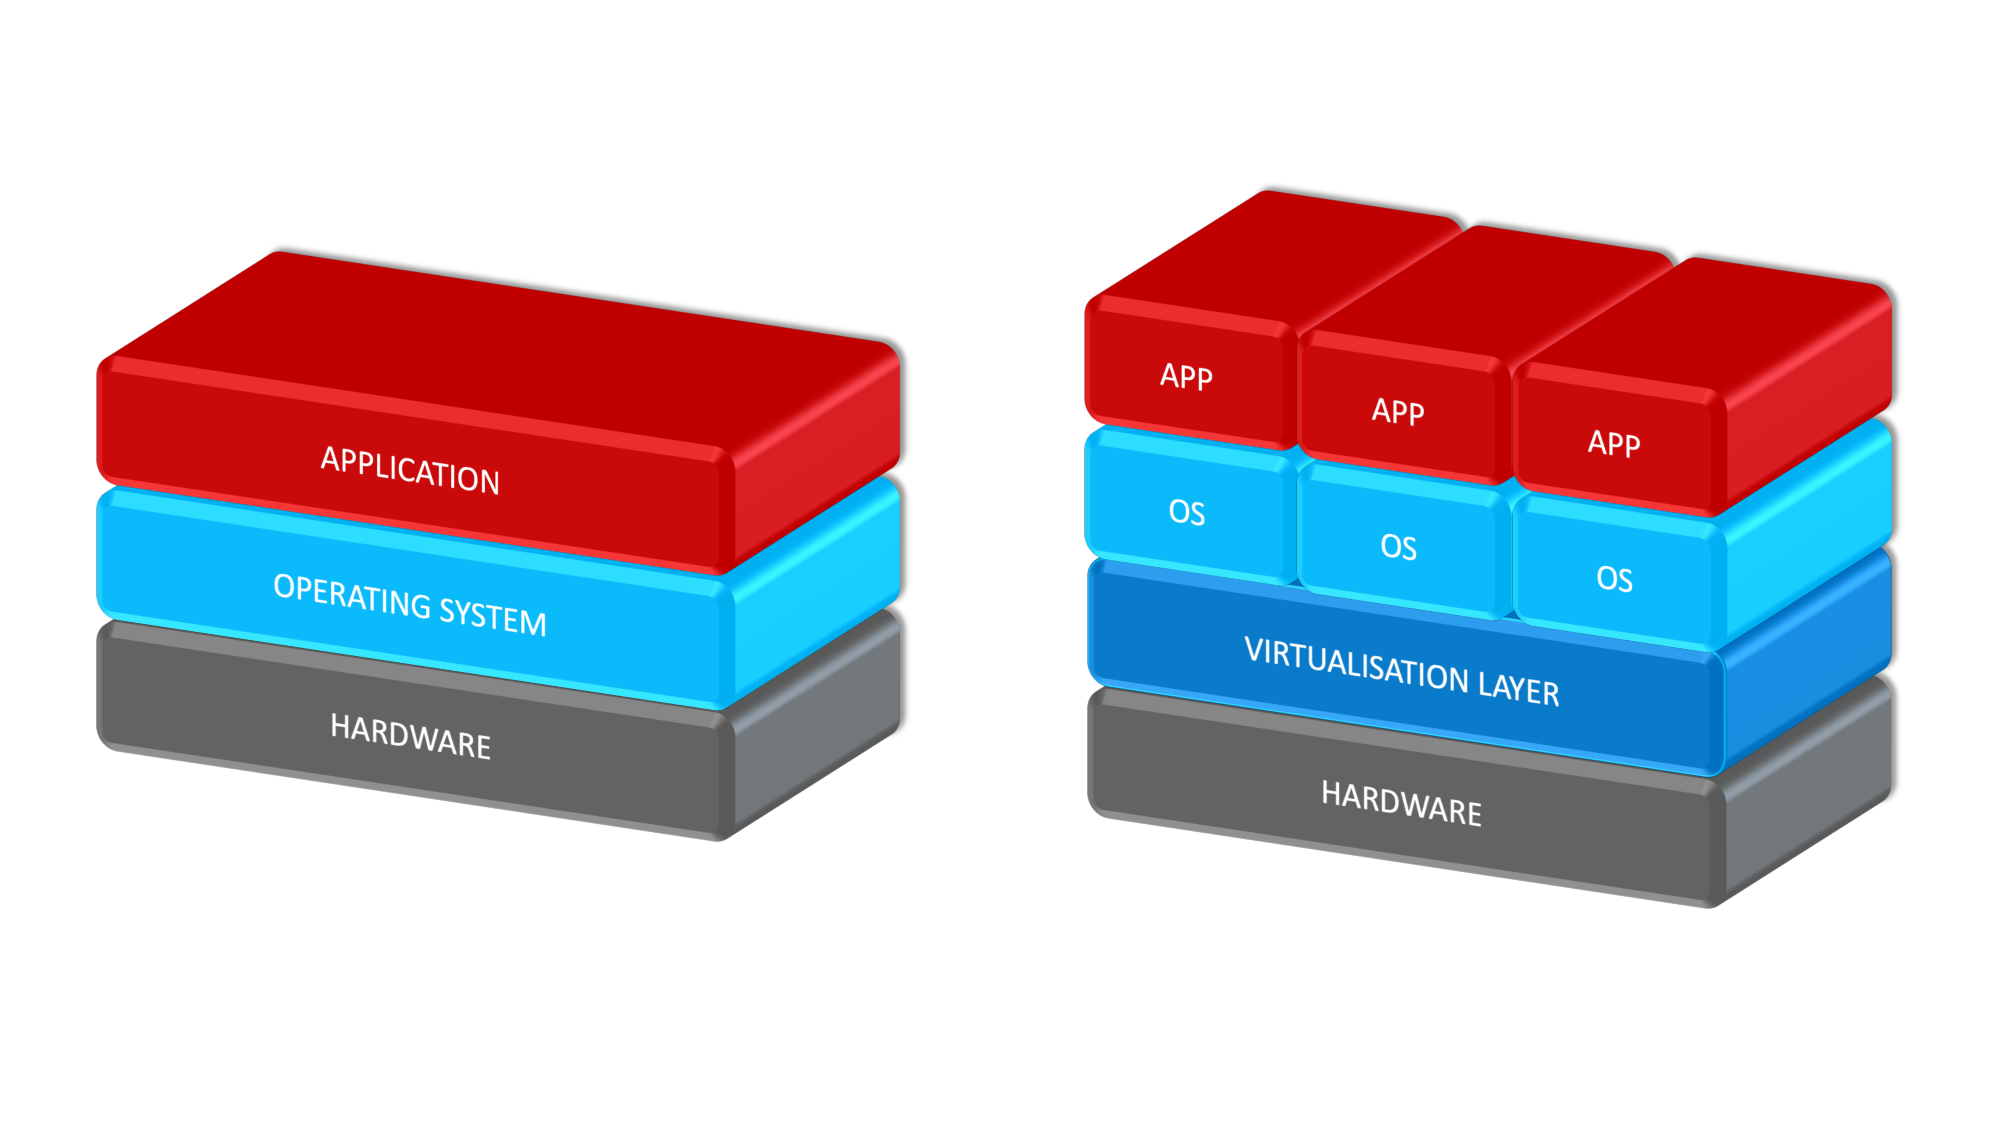
\includegraphics[width=10cm]{from_normal_to_virtualisation.pdf}\\
  \caption{Traditional architeture vs. virtualised architecture}
  \label{fig:virtualisation}
\end{figure}

\begin{figure}[h]
  \centering
  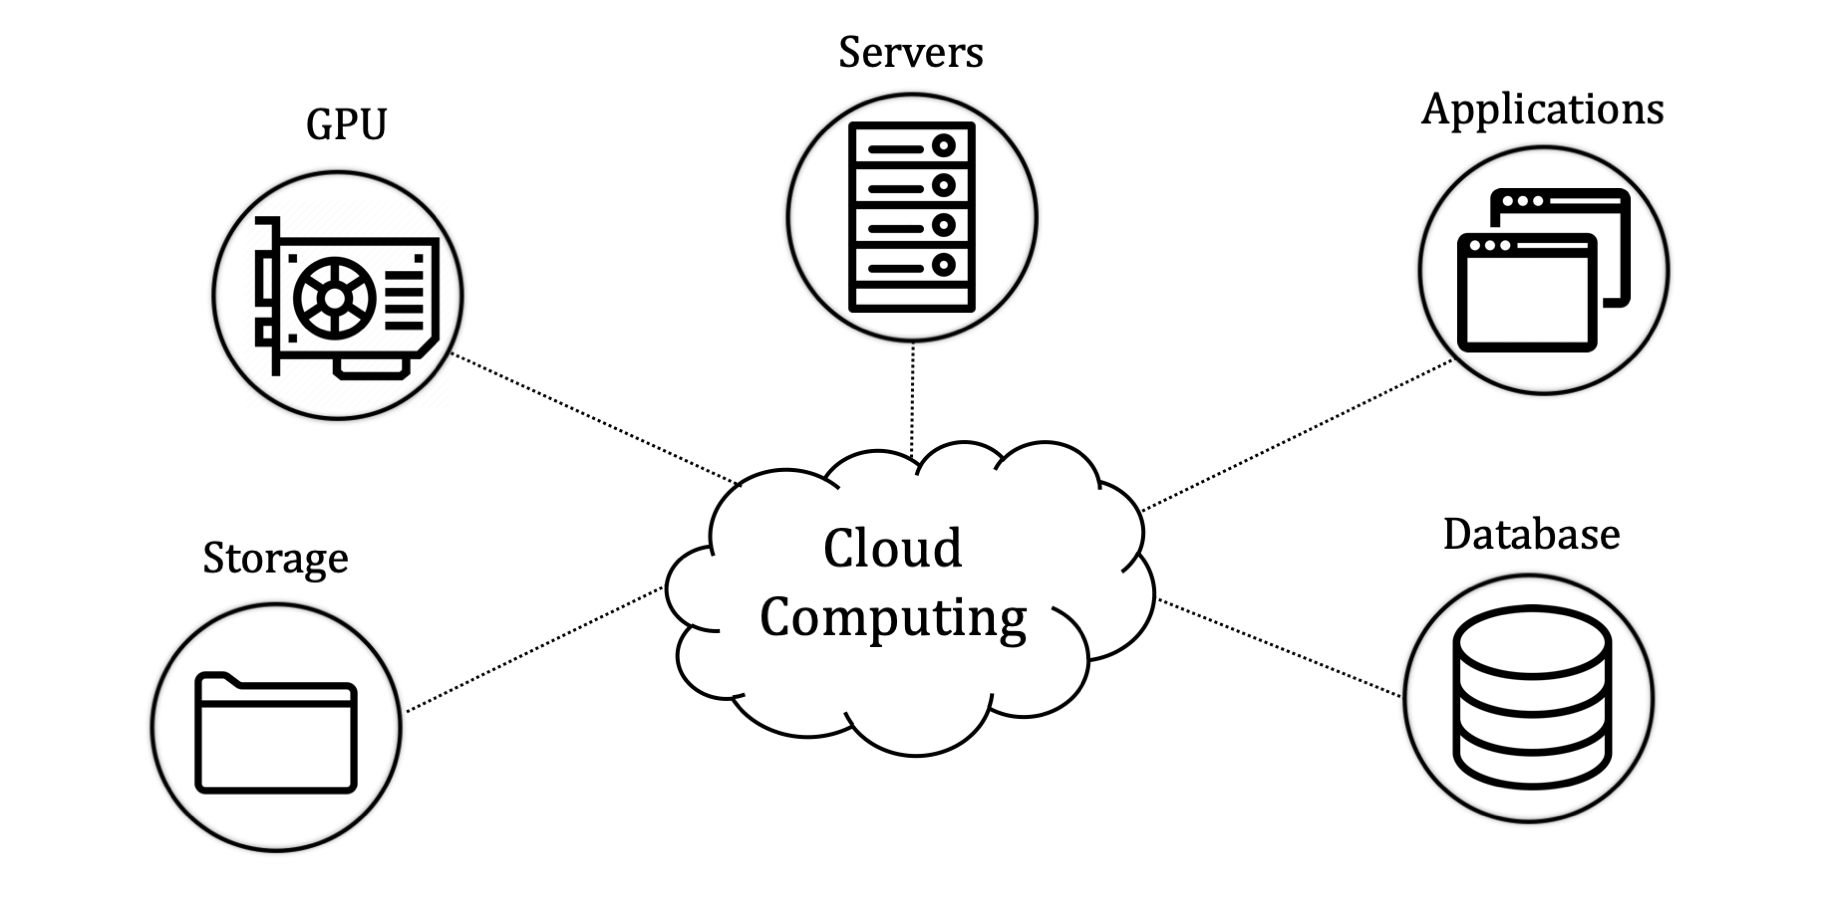
\includegraphics[width=15cm]{cloud.png}\\
  \caption{Traditional architeture vs. virtualised architecture}
  \label{fig:cloud}
\end{figure}


\section{Deep Learning \label{sec:deep-learning}}
\subsection{Neural Networks \label{sec:neural-networks}}
\begin{figure}[h]
  \centering
  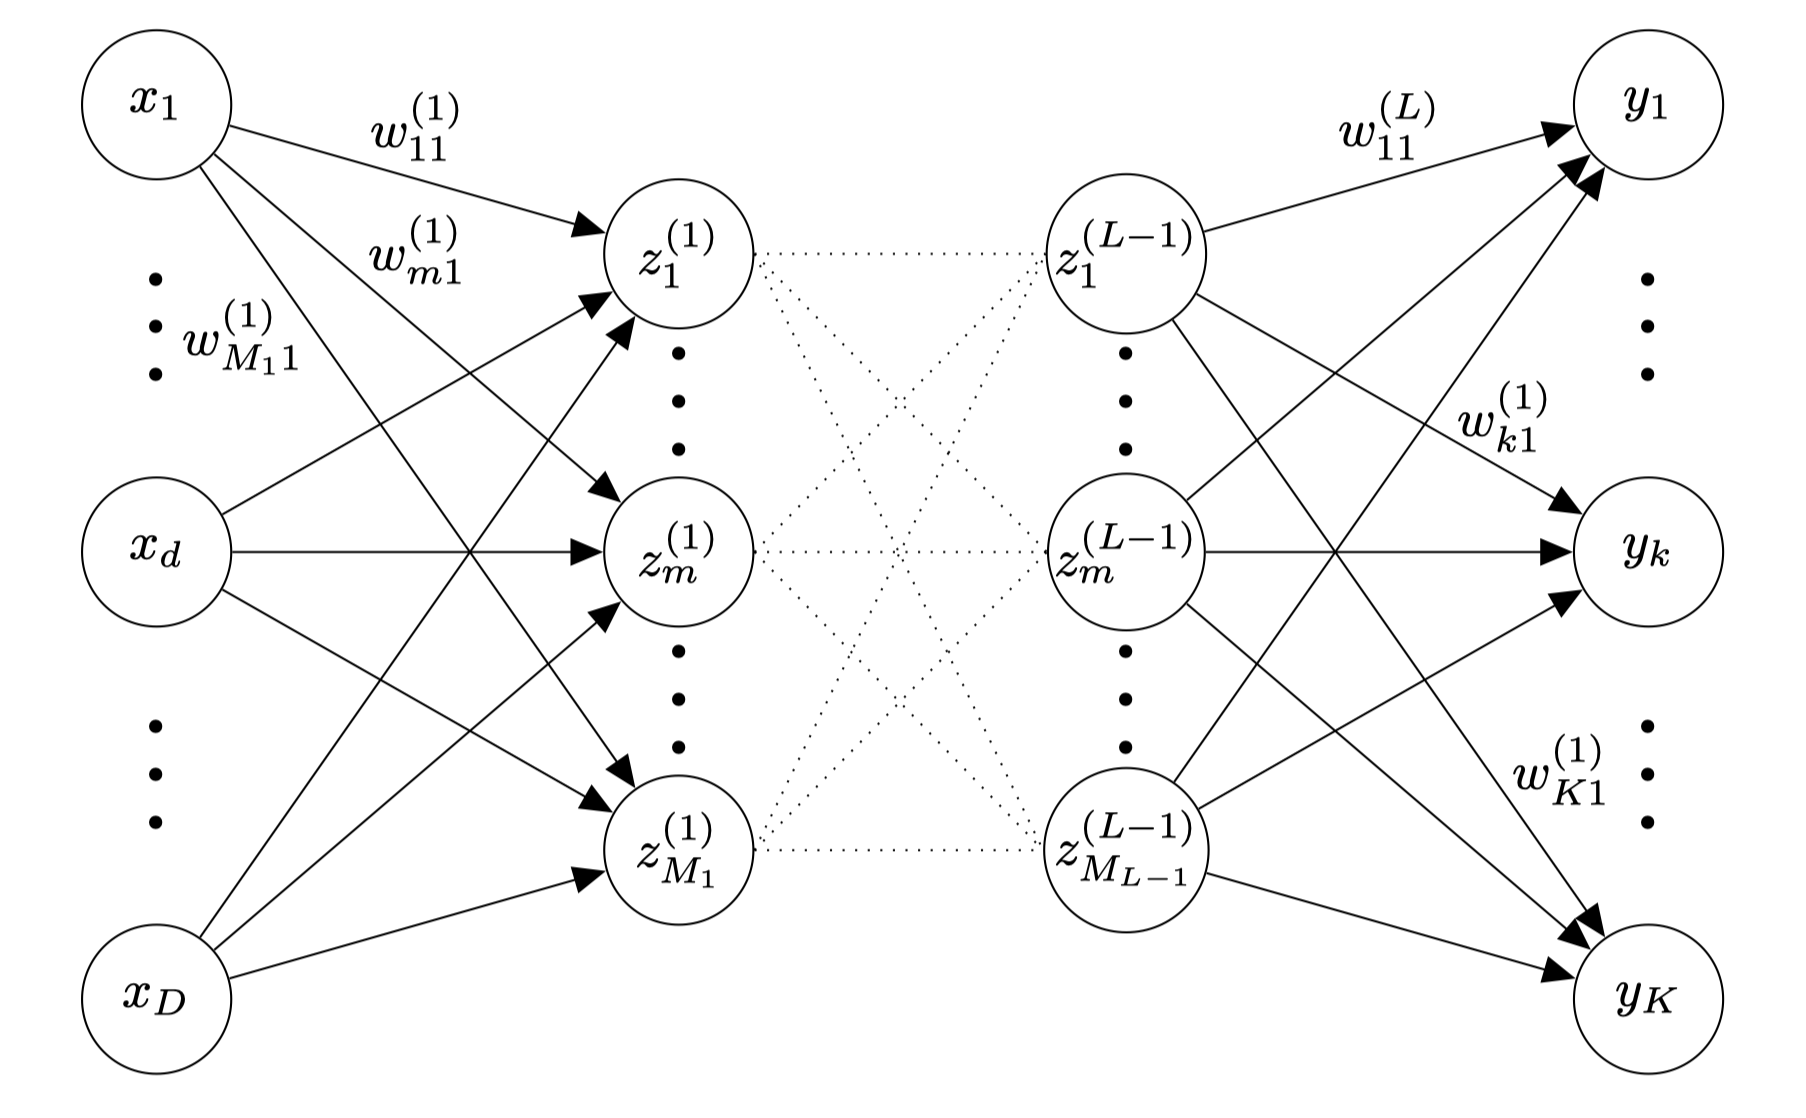
\includegraphics[width=15cm]{neural_network.png}\\
  \caption{A neural network \cite{hallmachinelearning}.}
  \label{fig:neural_network}
\end{figure}
Neural networks are self-learning systems that constitute a subcategory of machine learning. By analysing training examples, it learns to compute a functional relationship between an input and an output \cite{sibi2013analysis}. Figure \ref{fig:neural_network} is an illustration of a classical feed-forward neural network. It consist of \textit{neurons} and \textit{weights} connecting the neurons. There are three types of neurons: Each input value maps to an \textit{input} neuron depicted as $x_n$. \textit{Hidden} neurons, depicted as $z_i$ are predictors created by mathematical functions and the \textit{output} neurons, depicted as $y_k$ gather given predictions and compute the output \cite{hallmachinelearning}. Given data pairs $(x_1, t_1), ..., (x_N, t_N)$ with $x_n \in \mathbb{R}^D$ being input data, mapping to $D$ input neurons, and $t_n \in \mathbb{R}^K$ being target data. Each component $x_n$ is fed to one input neuron. If $L$ is the number of layers, then there are $L-1$ hidden layers. The network's latent variables of the hidden neurons are denoted by $z_m^{(l)}$. When data is being forwarded through the network, with the goal of obtaining a prediction from the network, the following formulas are relevant and describe every step through the network. The result of a complete forward propagation is denoted by activation \ref{eq:activation}:

\begin{equation}\label{eq:activation}
	a_j^{(l)} = \sum_{i=1}^{M_{l-1}}w_{ji}^{(l)}z_i^{(l-1)} = \bold{w}_j^{(l)^T} \bold{z}^{(l-1)}	
\end{equation}

On the result of this computation, an \textit{activation function} is applied as in \ref{eq:zj}. There exists a variety of activation functions, depending on the use case. Activation functions transform the activation of output neurons as in \ref{eq:activation} into an output signal \cite{sibi2013analysis}. For \textbf{regression} problems, the linear activation function $h(x)=x$ can be used. For \textbf{multi-classification} problems, where $t_n$ is a set of classes, the softmax function $\sigma(a)_j= \frac{e^{a_j}}{\sum_{k=1}^Ke^{a_k}}$ is used \cite{hallmachinelearning}.

There are more cases, but regression and multi-classification are the most relevant here, as they are used in chapter \ref{cha:concept}.

\begin{equation} \label{eq:zj}
	z_j^{(l)} = h_l(a_j^{(l)}) = h_l\Big(\bold{w}_j^{(l)^T} \bold{z}^{(l-1)}\Big)	
\end{equation}
If $l=1$, then equations \ref{eq:aj1} and \ref{eq:zj1} hold:

\begin{equation} \label{eq:aj1}
	a_j^{(1)}=\bold{w}_j^{(1)^T}\bold{x}
\end{equation}

\begin{equation} \label{eq:zj1}
	z_j^{(1)}=h_1\Big(\bold{w}_j^{(1)^T}\bold{x}\Big)
\end{equation}
If $l=L$, then every $y_k$ can be obtained in the following way:

\begin{equation}
	y_k = h_L(a_k^{(L)}) = h_L\Big( \bold{w}_k^{(L)^T} \bold{z}^{(L-1)} \Big)
\end{equation}

The result $y_k$ of the computation of $x_k$ is then compared to the real value $t_k$ using an \textit{error function}. Mean Squared Error $MSE = \frac{1}{n} \sum_{i=1}^n (t_k-y_k)^2$ can be used for regression problems, calculating the average squared difference between the estimated and the actual values, and Cross-Entropy $-\sum_{c=1}^My_{o,c} \: \log(p_{o,c})$ for multiclass classification, calculating the separate loss for each class label per observation. The obtained values are then fed into the \textit{back propagation algorithm}, updating weights $w_j$, thus trying to minimise the error. 


\begin{comment}
Figure \ref{fig:simple_neural_network} shows a simple neural network with three input features $v_1, v_2, v_3$. The output neuron is composed of the forward propagation function given by the weighted sums of neuron values, where the weights are $w_i$, and the activation function given by $h$. There exists a large variety of activation functions in use, depending on the given use case. The learning process of a neural network consists of learning the weights

Training of a neural network happens through 
Training of a neural network can be done in an \textit{unsupervised} and \textit{supervised} manner. Supervised training of 
The complexity of neural networks can be increased by adding more neurons and additional layers, making it possible to process larger input and potentially receive better results in prediction. The concept of the traditional feedforward neural networks is subject to constant architectural enhancement. 

Through the surge of available cheap computing power, deep learning models with high numbers of layers of neurons can be trained on large amounts of data. Also, the concept of the traditional neural network is constantly being 
\end{comment}



\subsection{LSTM networks \label{sec:lstm}}
\begin{figure}[h]
  \centering
  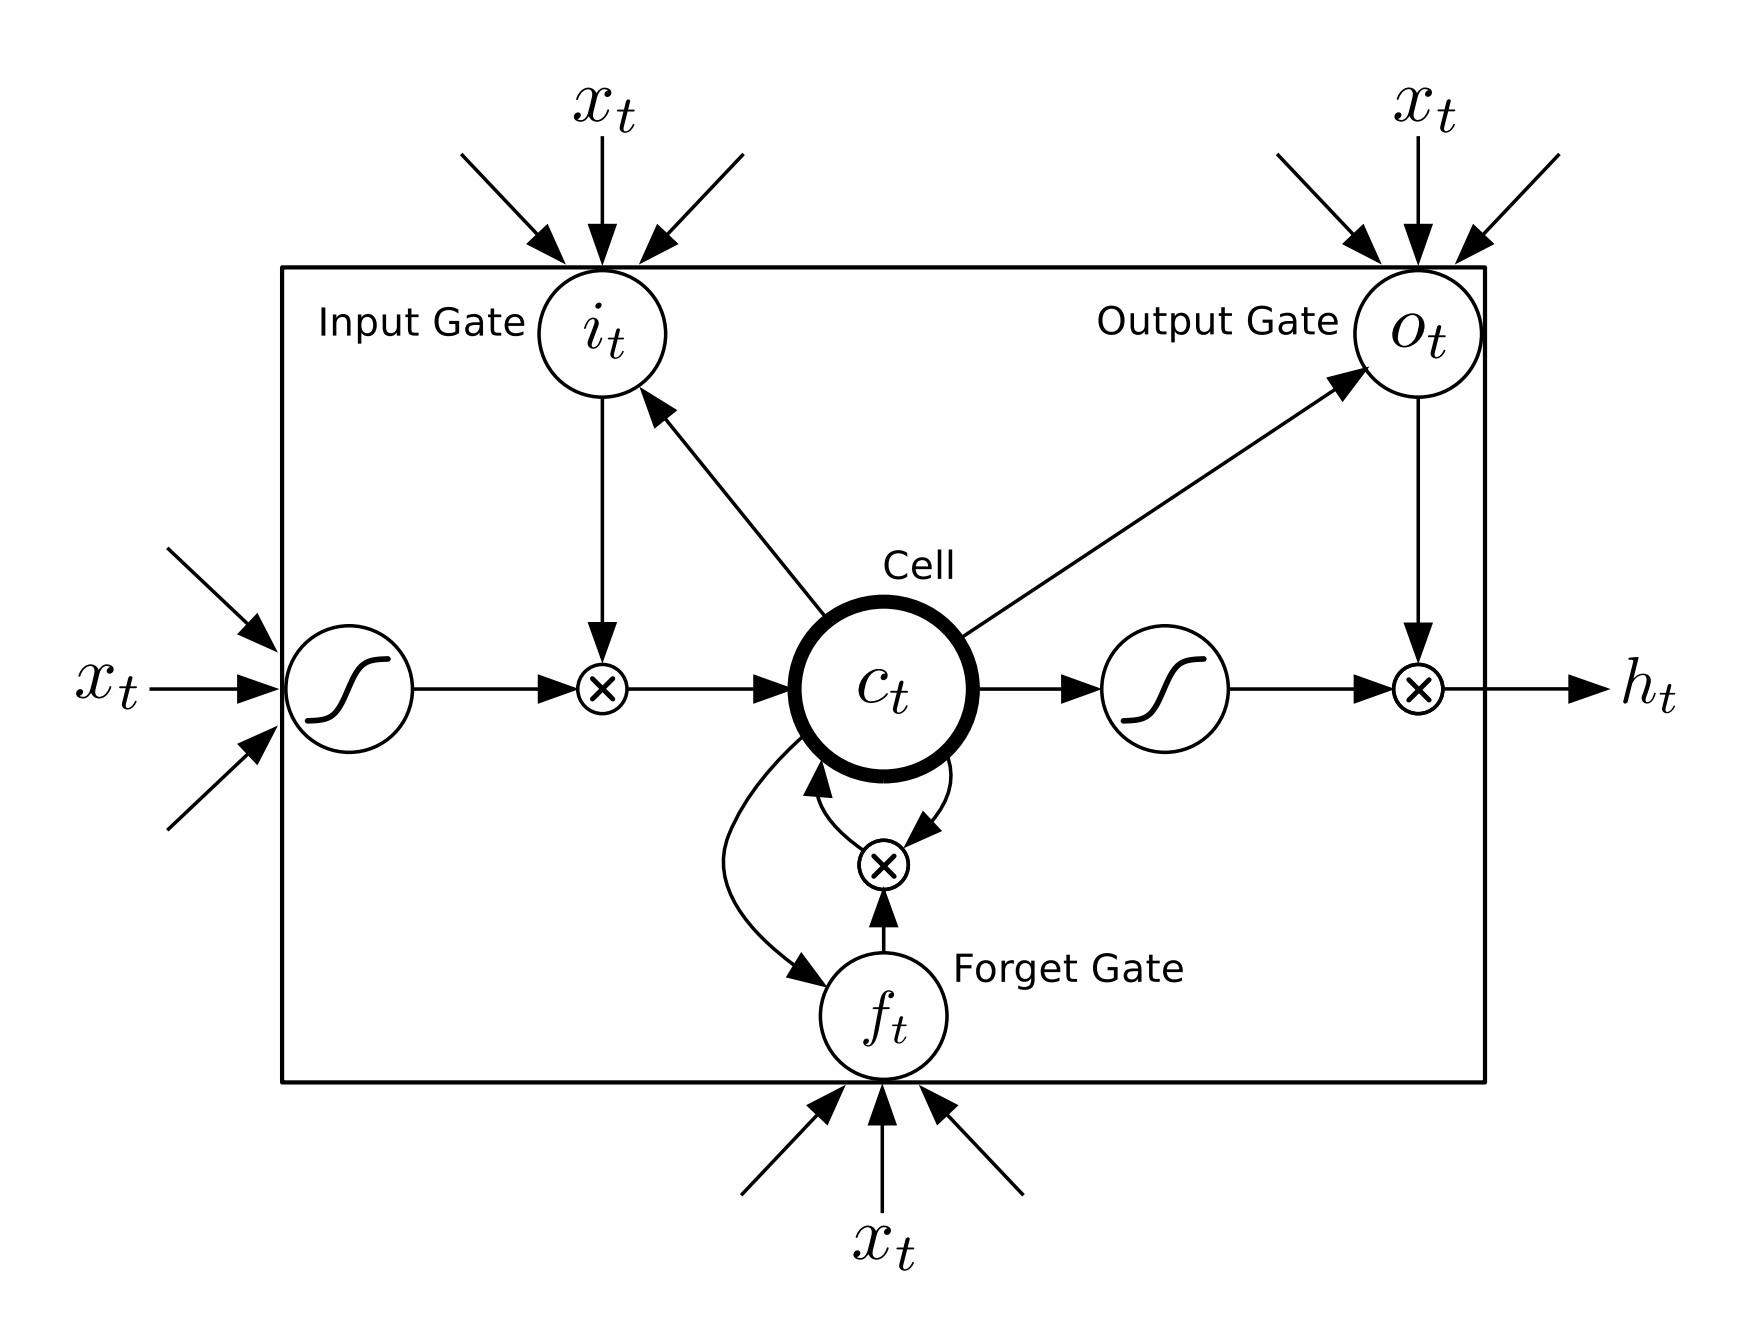
\includegraphics[width=10cm]{LSTM.png}\\
  \caption{LSTM block \cite{graves2013speech}}
  \label{fig:lstm_blocks}
\end{figure}


Recurrent neural networks (RNN) with Long Short-Term Memory (LSTM) are a widely-used effective model to tackle learning problems on sequential data. Being a general model, they do not have be to be adapted to a specific problem like earlier methods, thus allowing them to produce state-of-the-art results for problems like language modeling \cite{peters2018deep}, anomaly detection \cite{du2017deeplog} amongst others.

The core of the LSTM architecture is memory cell which maintains its state over time, in combination with gating units, which control the information flow \cite{greff2016lstm}, allowing it to remove or add information. The traditional LSTM architecture was first described by \cite{graves2005framewise}. The schematic structure of LSTM blocks is depicted in figure \ref{fig:lstm_blocks}. 

The first step is expressed through equation \ref{eq:f_t}. It is a forget gate, which considers the previous hidden state input $h_{t-1}$ and the current input $x_t$, and outputs a vector of numbers between 0 (forget: value should be multiplied by 0) and 1 (keep: multiply value by 1), one for each element from the previous cell state $c_{t-1}$. Next, equation \ref{eq:i_t} computes, which values to update. Equation \ref{eq:hatC_t} creates a vector of candidate values $\hat{c}_t$ for the new state $c_t$. In equation \ref{eq:C_t}, the previous state is multiplied with $f_t$, in order to keep or forget elements, adding the new candidate values $\hat{c}_t$ multiplied by the degree updating $i_t$. As the last two steps, in equation \ref{eq:o_t}, the output is computed by applying a sigmoid on the cell state, to decide which parts to output. Then, in equation \ref{eq:h_t}, a tanh is applied on the cell state $c_t$, which is multiplied by the output of the sigmoid gate $o_t$ \cite{colahlstm} \cite{graves2013speech}.

\begin{equation} \label{eq:f_t}
	f_t = \sigma(W_{xf}x_t + W_{hf}h_{t-1} + W_{cf}c_{t-1} + b_f)
\end{equation}

\begin{equation} \label{eq:i_t}
	i_t = \sigma(W_{xi}x_t + W_{hi}h_{t-1} + W_{ci}c_{t-1} + b_i)
\end{equation}

\begin{equation} \label{eq:hatC_t}
	\hat{c}_t = \tanh(W_{xc}x_t + W_{hc}h_{t-1} + b_c)
\end{equation}

\begin{equation} \label{eq:C_t}
	c_t = f_t c_{t-1} + i_t \hat{c}_t
\end{equation}

\begin{equation} \label{eq:o_t}
	o_t = \sigma (W_{xo}x_t + W_{ho}h_{t-1} + W_{co}c_t + b_o)
\end{equation}

\begin{equation} \label{eq:h_t}
	h_t = o_t \tanh(c_t)
\end{equation}


\begin{comment}
\begin{equation} \label{eq:f_t}
	f_t = \sigma(W_f \cdot [h_{t-1},x_t] + b_f)
\end{equation}

\begin{equation} \label{eq:i_t}
i_t = \sigma(W_i \cdot [h_{t-1},x_t] + b_i)
\end{equation}

\begin{equation} \label{eq:hatC_t}
\hat{C}_t = \tanh(W_C \cdot [h_{t-1},x_t] + b_C)
\end{equation}

\begin{equation} \label{eq:C_t}
C_t = f_t \cdot C_{t-1} + i_t \cdot \hat{C}_t
\end{equation}

\begin{equation} \label{eq:o_t}
o_t = \sigma (W_o [h_{t-1}, x_t] + b_o)
\end{equation}

\begin{equation} \label{eq:h_t}
h_t = o_t \cdot \tanh(C_t)
\end{equation}
\end{comment}


\subsection{Bidirectional LSTM networks \label{sec:bi-lstm}}
\begin{figure}[h]
  \centering
  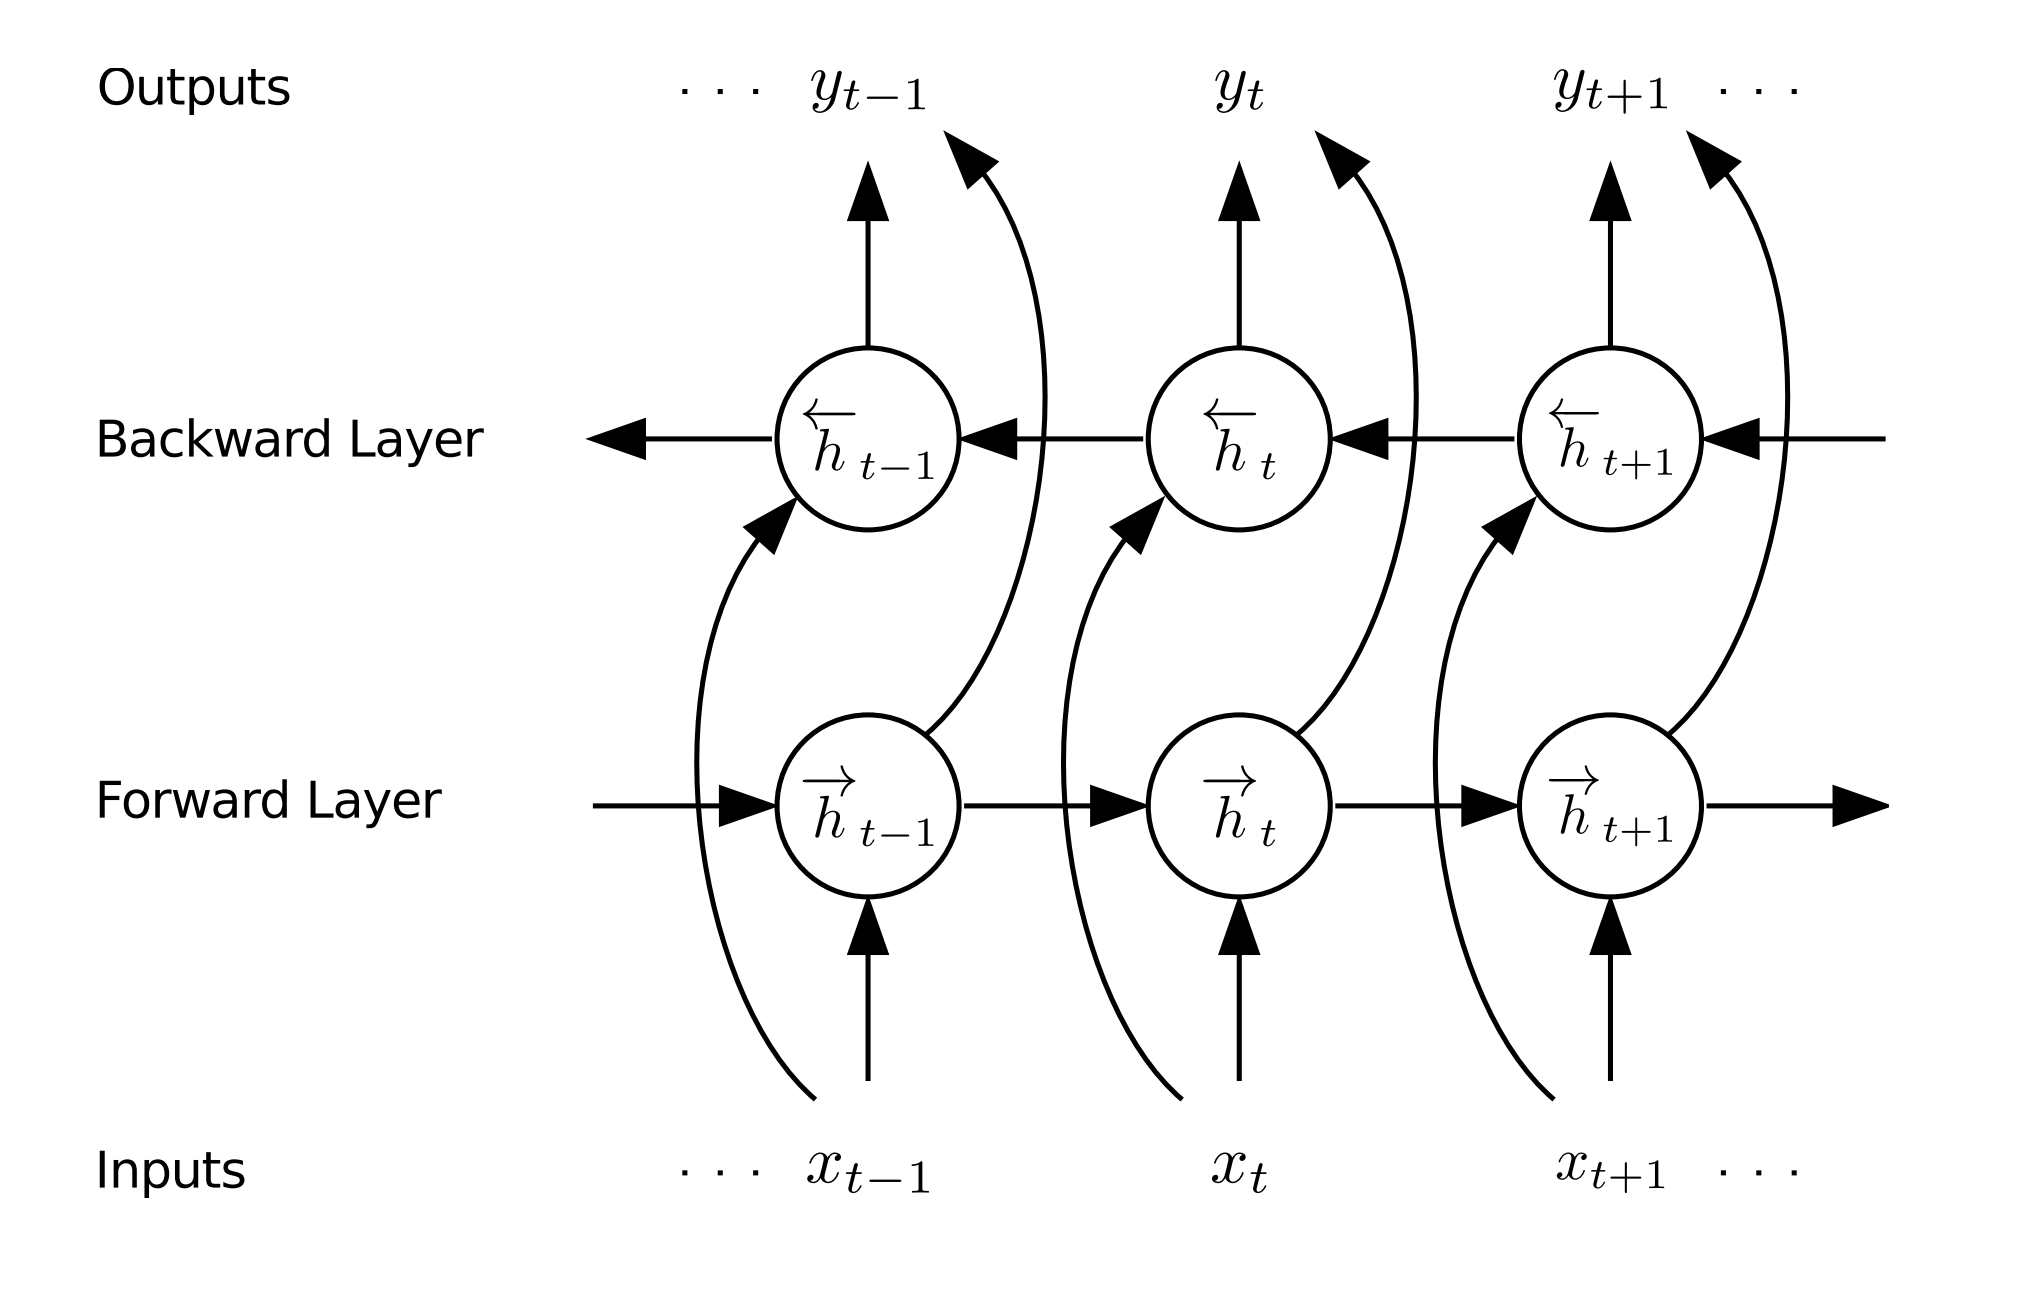
\includegraphics[width=10cm]{Bi-LSTM} \\
  \caption{Bi-directional LSTM \cite{graves2013speech}.}
  \label{fig:bi-lstm}
\end{figure}
In a sequence prediction task, in which one has access to both past and future input features for a given point in time, a bidirectional LSTM network as depicted in \ref{fig:bi-lstm} can be applied as proposed by Graves et al. \cite{graves2013speech}. In this way, it is possible to make us of past features via the forward state and future features via the backward states. Forward and backward passes are executes similarly to 



The forward and backward passes over the unfolded network over time are carried out in a similar way to regular network forward and backward passes, except that we need to unfold the hidden states for all time steps. We also need a special treatment at the beginning and the end of the data points. In our implementation, we do forward and backward for whole sentences and we only need to reset the hidden states to 0 at the begging of each sentence. 




\section{Anomaly Detection \label{sec:anomaly-detection}}
\textit{Anomaly detection} describes the general problem of finding subsets or patterns in data, that do not conform to a defined notion. These patterns are often referred to as outliers or anomalies.

Anomalies can arise in datasets for various reasons, like system errors, fraud or malicious activities. It often might appear to be straight-forward to define normal regions, and declare all data laying outside of these regions as anomalies. Unfortunately, finding these normal regions is in fact very difficult, since it might not always be possible to capture the nature of \textit{normal} data in its completeness, due to lacking data or the unsharp border of normal and abnormal. Consider figure \ref{fig:anomaly_dataset}, which illustrates the presence of normal regions and anomalies in a dataset. The datapoints in the regions $D_1$ and $D_2$ are considered normal, since the majority of observations lie in these regions. Points that are sufficiently far away, like the points in regions $A_1$ and $A_2$ are considered anomalies. But consider also the points $B_1$. Should they be marked as normal or abnormal? Are the borders around $D_1$ and $D_2$ correct, or are they not sufficiently broad, due to the lack of enough normal training examples? 
Additionally to the difficulty of finding correct division of normal and abnormal, normal behaviour can be subject to constant evolution in a dynamic system, thus making previous definitions of \textit{normal} behaviour wrong, obsolete or incomplete. Additionally, it is often hard or impossible to obtain labeled data for the desired domain, thus hindering the training and verification of a model \cite{chandola2009anomaly}.

Due to the difficulties arising from the aforementioned constraints, solutions to the problem of anomaly detection are usually very domain-specific, influenced by the form in which data is available, labeled or unlabeled and the form of anomalies which are to be detected. Solutions presented by researchers feature techniques from various fields, including data mining, statistics, machine learning which are applied to the domain in question \cite{chandola2009anomaly}. Figure \ref{fig:anomaly_technique} outlines the central steps involved in finding an appropriate anomaly detection technique to a given problem.


\begin{figure}[h]
  \centering
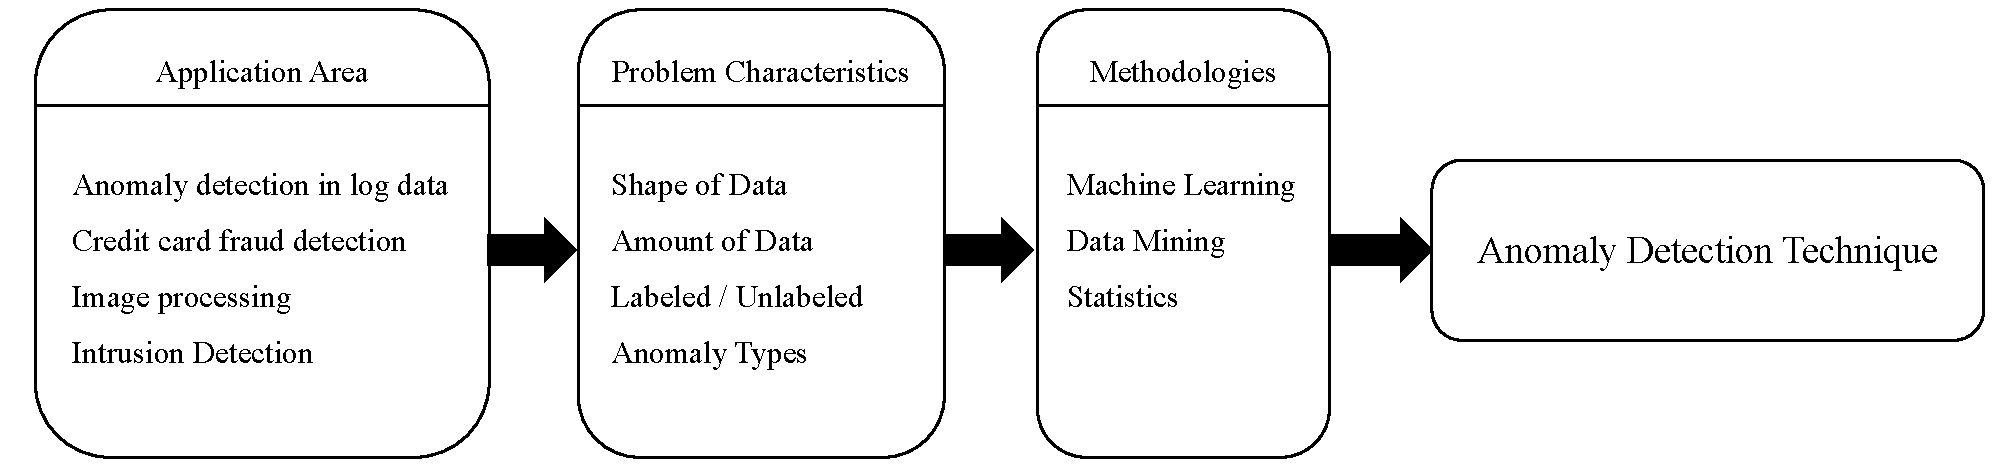
\includegraphics[width=15cm,height=3.5cm]{anomaly_detection_techniques.pdf}\\ 
  \caption{Schema of the development of an anomaly Detection technique \cite{chandola2009anomaly}.}
  \label{fig:anomaly_technique}
\end{figure}

\begin{figure}[h]
  \centering
  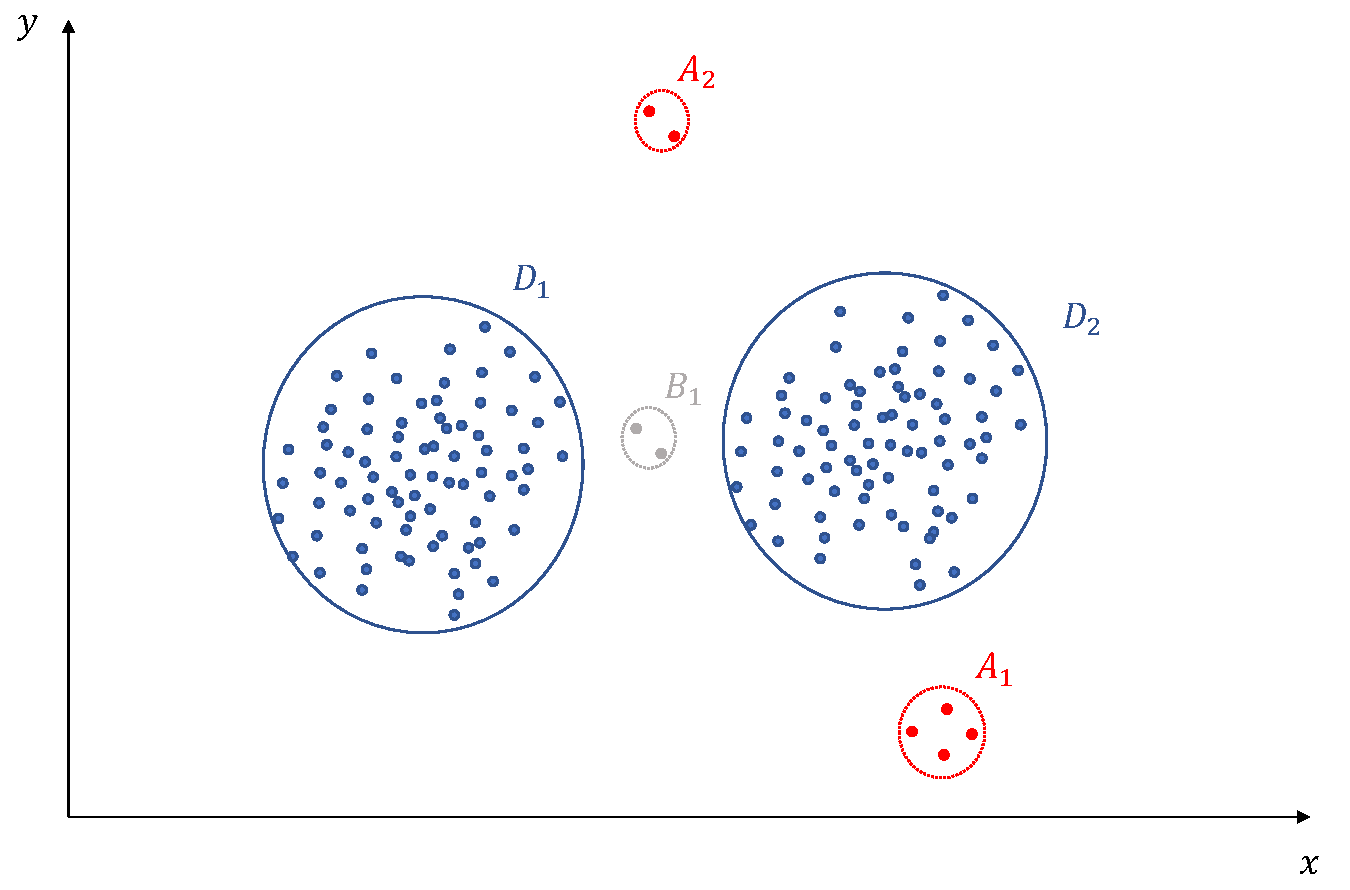
\includegraphics[width=15cm]{anomalies.pdf}\\
  \caption{Example of anomalies in a dataset.}
  \label{fig:anomaly_dataset}
\end{figure}


\section{Natural Language Processing \label{sec:natural-language-processing}}

Natural language processing (NLP) involves the engineering of computational models to solve practical problems in understanding human languages. Having initially relied on processing involving statistics, probability and machine learning, the recent boost in available computational power with GPUs, allowed deep learning to raise the bar for many NLP-tasks. NLP can be broadly divided into two categories, namely \textit{base concepts} which deal with the fundamentals of understanding language, and concrete applications by means of these very concepts, although the border between the two is often fluent. Base concepts include \textit{language modelling}, \textit{morphological processing} (find segments within words), \textit{syntactic processing} (how different words and phrases relate to each other within a sentence) and \textit{semantic processing} (understanding the meaning of words), whereas applications include areas such as text translation, classification of documents, summarisation of texts, extraction of information and many more.
\subsection{Word embeddings}
Language modelling can be viewed as an essential piece of probably any practical application of NLP. Generally speaking, it involves creating a model to predict words given previous words by finding appropriate representations for words through analysing the relations of words within their context. Numeric vectors, which represent single words, obtained by language model techniques are called \textit{word embeddings} \cite{otter2020survey}. For example, the word "Olympics" appears often in the context or close to words like "athlete", "running" or "tournament" but rather rarely next to words like "microphysics" or "chicken". These relationships can be translated into a vector that describes how the word "Olympics" is used within a language \cite{mittechnologyreviewkingqueen}. Word embeddings can be retreived either by Principle Component Analysis or by using deep neural network models and capturing their internal states.
\subsection{Bert \label{Bert}}
The functionality of a language representation model will be outlined on the basis of Bert (\textbf{B}idirectional \textbf{E}ncoder \textbf{R}epresentations from \textbf{T}ransformers) by Devlin et al. \cite{devlin2018bert}. The model architecture is a multi-layer bidirectional Transformer encoder. The encoder maps an input sequence of symbol representations to a sequence of continuous representations. The transformer architecture introduces self-attention and fully connected layers on top of the encoder structure, which has been shown to be superior in quality and is significantly cheaper to train \cite{vaswani2017attention}.

Training includes two steps: \textit{pre-training} and \textit{fine-tuning}. Pre-training involves training on unlabelled data over various pre-training tasks. Finetuning then uses the weights initialised with the parameters obtained from pre-training, re-calibrating them using labelled data.

For pre-training, they extract sentences from a large unlabelled corpus like English Wikipedia. The obtained sentences are then transformed into tokens, and separated by pre-defined separation symbols, \verb![CLS]! for the beginning of a sentence, \verb![SEP]! for the ending of sentences as illustrated in figure \ref{fig:bert}. They then proceed with the first task, namely Masked Language Model (MLM). For this purpose, they mask 15\% of words with the special \verb![MASK]! token, and then predict these tokens. The second task is Next Sentence Prediction (NSP), where sentences \verb!A! and \verb!B! are separated with the aforementioned \verb![SEP]! token, as it can be again seen in figure \ref{fig:bert} are marked with the label \verb!isNext! if \verb!B! follows \verb!A! or \verb!notNext! if the following sentence is a random sentence, with both cases occurring 50\% of the time. After the computationally expensive pre-training is done, taking 4 days of training on 16 cloud TPUs for one language \cite{googlebert}, fine-tuning can be done on any downstream NLP task in at most one hour on one cloud TPU, for example the Stanford Question Answering Dataset (SQuAD v1.1) by Rajpurkar et al. \cite{rajpurkar2016squad}, a collection of 100k crowd-sourced question/answer pairs, or the General Language Understanding Evaluation (GLUE) benchmark by Wang et al. \cite{wang2018glue}, which involves various natural language understanding tasks. 


\begin{figure}[h]
  \centering
  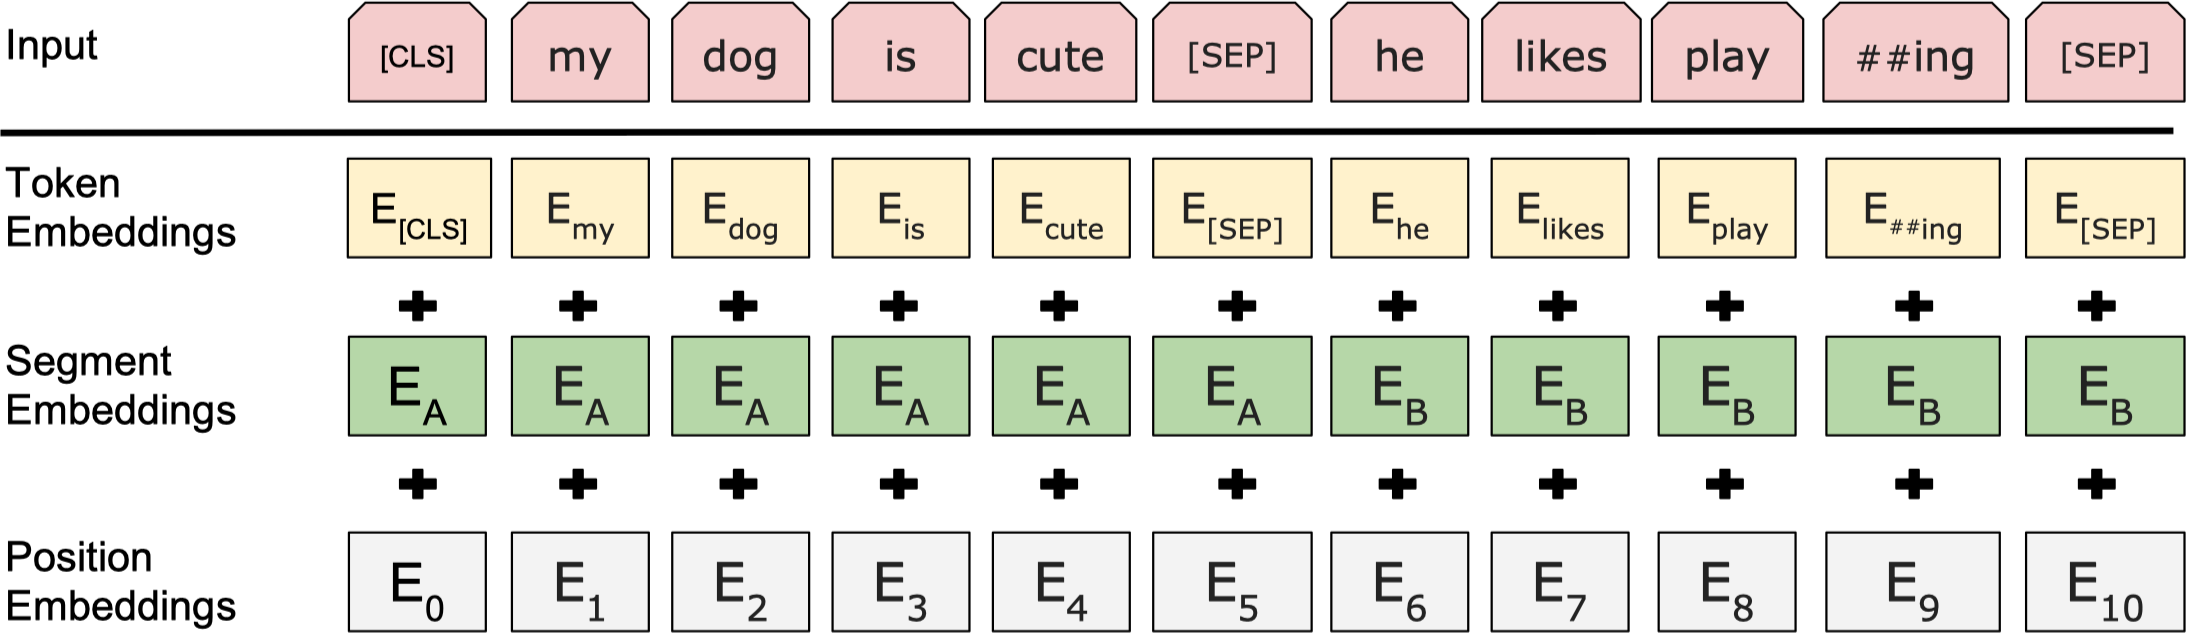
\includegraphics[width=15cm]{bert2.png}\\
  \caption{Bert}
  \label{fig:bert}
\end{figure}


\begin{comment}
\begin{figure}[h]
  \centering
  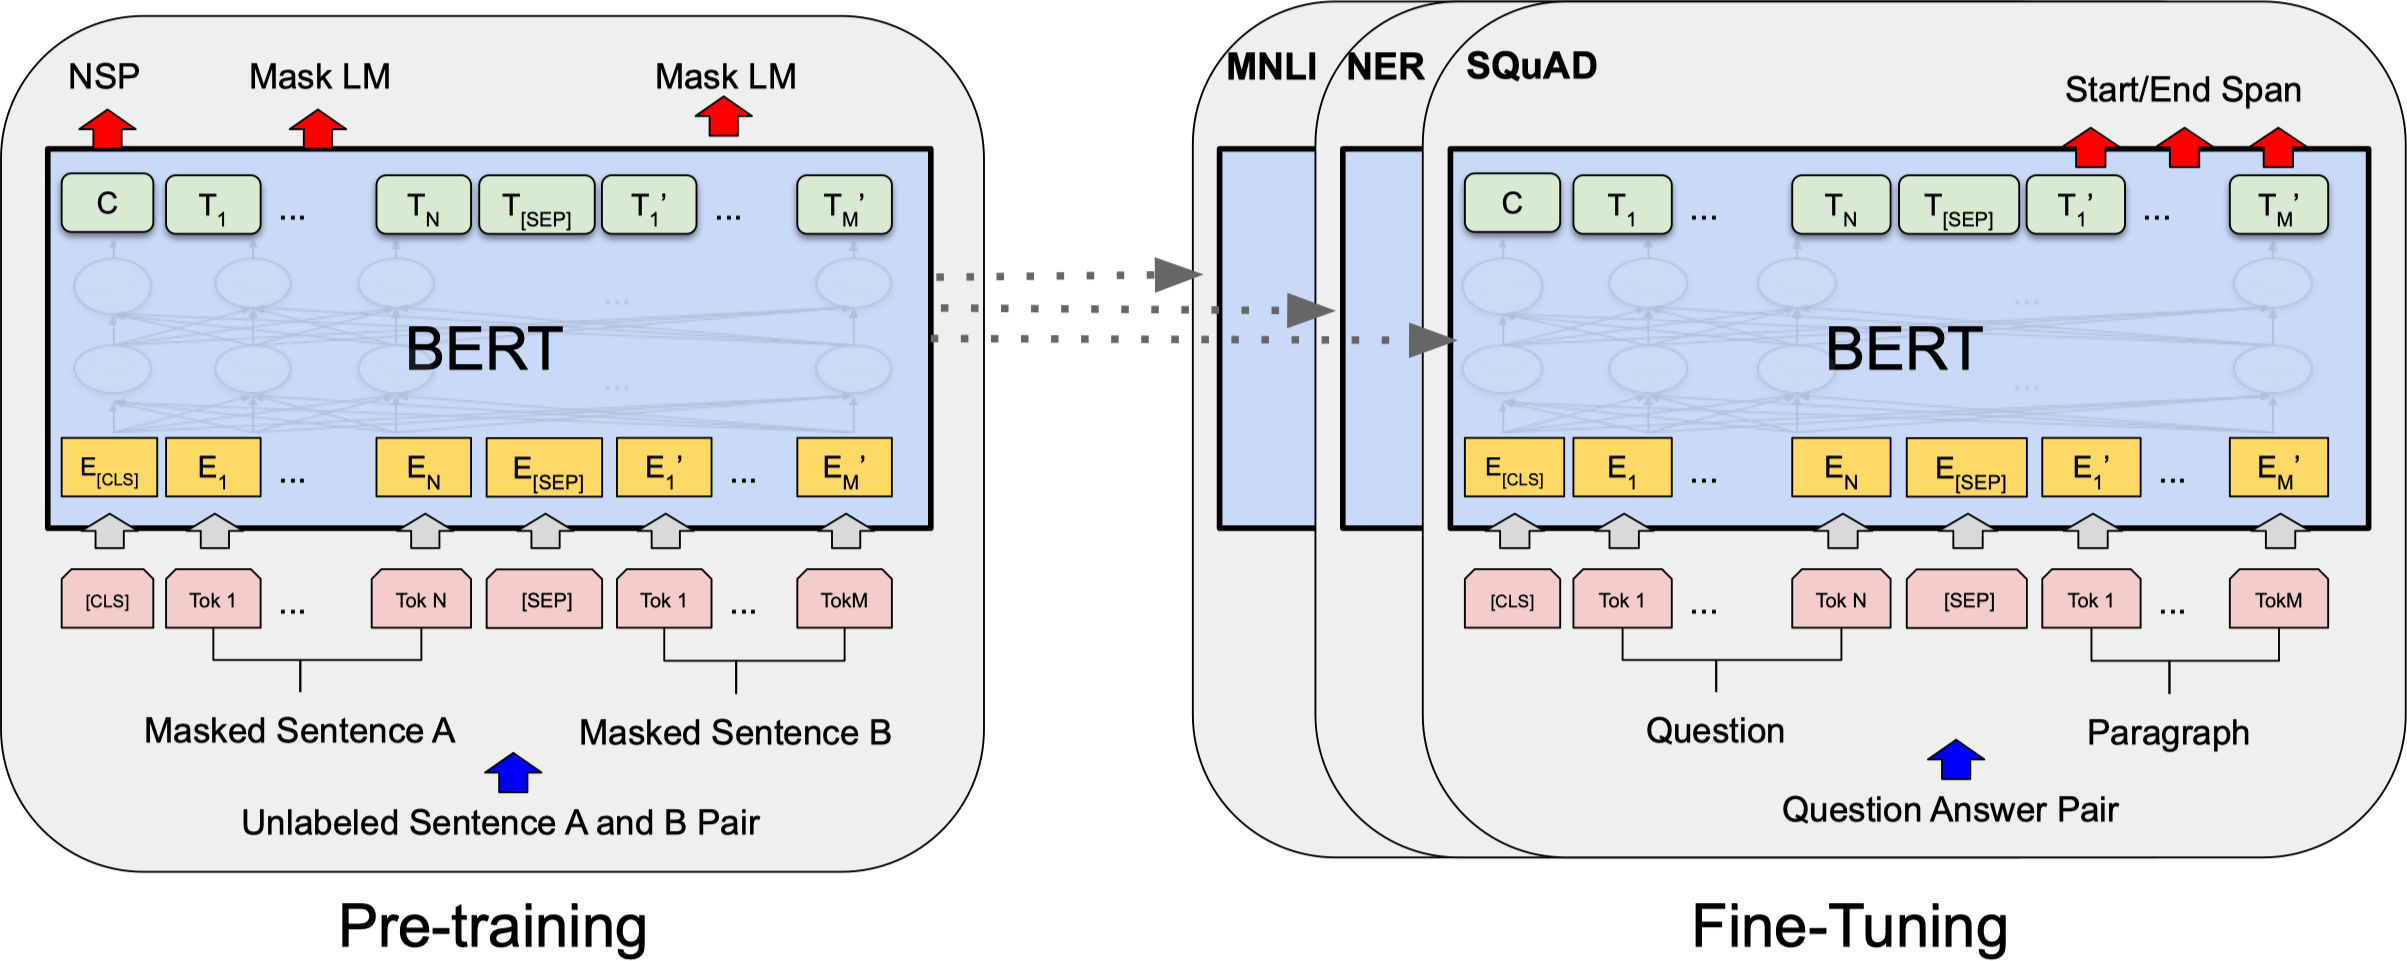
\includegraphics[width=15cm]{bert.png}\\
  \caption{Bert}
  \label{fig:bert}
\end{figure}
\end{comment}

\begin{comment}
Generally, there are two main categories of log sequence anomalies: sequential and quantitative anomalies \cite{meng2019loganomaly}. Programs are usually executed according to static sequences, and the order of the respective log statements that are being produced, is a result of these executions. A sequential anomaly occurred, when a given sequence departs from a pattern that has been defined as normal. Works in this area include DeepLog \cite{du2017deeplog}.
Additionally, program executions have constant linear relationships - these can be captured by the quantitative relationships of logs. If these relationships are not met under all circumstances, an anomaly has occurred. Existing works in the area include PCA based approaches over log message counter \cite{xu2010robust} \cite{xu2009detecting} and LogClustering \cite{lin2016log}, but there are also deep learning based approaches to learn sequences of logs, like DeepLog \cite{du2017deeplog}. The main limitation of these approaches is that they use log event template indices as input to predict sequences. 

To overcome the shortcomings of previous approaches, it is worthwhile to consider recent developments in natural language processing. In order for a machine to process information given in natural language, a suitable representation for the given text has to be found. Learning representations of words has been a dynamic area of research, using neural \cite{blitzer2006domain} \cite{devlin2018bert} \cite{radford2019language} \cite{merity2017regularizing} \cite{yang2017breaking}, statistical \cite{brown1992class} and other machine learning methods \cite{ando2005framework} \cite{pennington2014glove}. Recently, we have seen considerable improvements in both the (multi-) task solving capabilities and efficiency of deep learning approaches. Because of their capabilities of memorising sequential context in language, RNNs \cite{mikolov2010recurrent} have often been the architecture of choice \cite{merity2017regularizing} \cite{yang2017breaking} in the past years. Decidedly designed cells to memorise such context make them computationally expensive, making it difficult to scale to large corpora \cite{wang2019language}. The transformer architecture introduces self-attention and fully connected layers, which has been shown to be superior in quality and is significantly cheaper to train \cite{vaswani2017attention}. BERT \cite{devlin2018bert} and GPT-2 \cite{radford2019language} provide state of the art results in various NLP tasks. There exist a variety of practical applications, such as information retrieval \cite{manning2008introduction}, question answering \cite{tellex2003quantitative}, paraphrasing \cite{dolan2005automatically}, natural language inference \cite{bowman2015large}, document classification \cite{sebastiani2002machine}. They are trained in an unsupervised manner on publicly available datasets like Wikipedia, or millions of web pages accumulated in one dataset, to obtain a more diverse dataset \cite{radford2019language}. This allows them to achieve state of the art results in various language modeling tasks like question answering \cite{reddy2019coqa} or language inference without specific modifications of the model to solve a certain task \cite{devlin2018bert}, making them much more universally applicable than older approaches like word2vec \cite{mikolov2013distributed} or GloVe \cite{pennington2014glove}. There are recent studies \cite{zhang2019robust} \cite{meng2019loganomaly} which utilise such pre-trained word embeddings to provide a more meaningful representation of log events, being able to take into account their semantics. 
In this section, the necessity for anomaly detection with log events represented by word embeddings is further elaborated. For this purpose, the necessary methods like log parsing, 
Log messages are the result of the insertion of a variable part in a logging instruction (e.g. \textit{printf("Instance \%s shut down with errors, \%s)} in software code that is being output during execution. The constant parts can usually be found in source codes written by developers, while the variable parts are inserted dynamically during execution. As these logs are unstructured text, have to undergo certain pre-processing steps before they can be analysed for anomalies. Each log event can be parsed into a log template, leaving only the constant part, as it can be seen in figure \ref{fig:parsing}.
\end{comment}


\section{Log Parsing \label{sec:backgroundlogparsing}}
Due to the unstructured nature of log data, the first crucial step in anomaly detection on log data is parsing. Raw log messages consist of a constant and a variable part, with the constant part remaining identical for every occurrence, while the variable part records runtime information and varies among different event occurrences. The goal of log parsing is to separate the \textit{constant} and \textit{variable} part of a raw log message \cite{he2017towards}\cite{zhu2019tools}. Figure \ref{fig:parsing} shows how logging statements from Java source code are parsed. The logging statements variable parts \verb!block!, \verb!block.getNumBytes()! and \verb!inAddr! are dynamically interpreted at runtime and replaced by their respective values. The resulting log message is then printed with additional customisable values (timestamp, logging level and component) by the respective logging framework. The structured log is then produced by the log parser, separating the constant part, which is also called a \textit{template} (\verb!Received block <*> of size <*> from /<*>!) from the variable parts (\verb!blk_-562725280853087685, 67108864! and \verb!10.251.91.84!), replacing the variable parts inside the constant parts with a pre-defined token - "\verb!<*>!" in this example.

Log parsing is usually the first step in order to perform a log analysis task. Log parsing enables enables searching, filtering, grouping and mining of logs. Applications include usage analysis at Twitter \cite{lee2012unified} or workload modelling \cite{barham2004using}. Logs can also be used as data sources for performance modelling \cite{chow2014mystery} where performance improvements of a system can be validated using log data. A very prominent application of log parsing is anomaly detection. Since logs record execution information of a system, they are a valuable data source for identifying abnormal behaviour of a system \cite{zhu2019tools}.

There exist offline and online log parsers, offline meaning that it first reads and analyses the whole dataset first before applying the parsing model, while online parsers adjusts the parsing model gradually during the parsing process \cite{he2017drain}. Log parsers employ various concepts and techniques in order to parse logs - a few of them are summarised here:
\begin{itemize}
\setlength\itemsep{0em}
	\item \textit{Frequent Pattern Mining} involves finding sets of patterns, in this case templates, that appear frequently in a data set. The procedure can be outline as follows: Iterating over the log data several times, while building frequent sets of tokens, followed by grouping log messages in clusters, and then extracting event templates from each of the clusters.
	\item Log parsing can be viewed as a \textit{clustering} problem. All approaches can be roughly outlined as clustering templates hierarchically based on a defined metric, for example the weighted edit distance between pairwise log messages \cite{zhu2019tools}.
	\item Some proposed methods utilise special heuristics, 	exploiting the unique characteristics of log messages. IPLoM first identifies frequent words occurring more frequently than a threshold value, then extracts combinations of these words that occur in each line in the data set, marking them as cluster candidates, and finally selecting the candidates the occur more often than a threshold value as clusters \cite{makanju2009clustering}. Drain employs a parse tree with fixed depth. It first preprocesses the incoming messages with regular expressions based on domain knowledge, then search a log group for that message, with log groups being leaf nodes. If a suitable group is found, it matches the message to that group, if not, then a new group is created \cite{he2017drain}.
\end{itemize}


\begin{figure}[h]
  \centering
  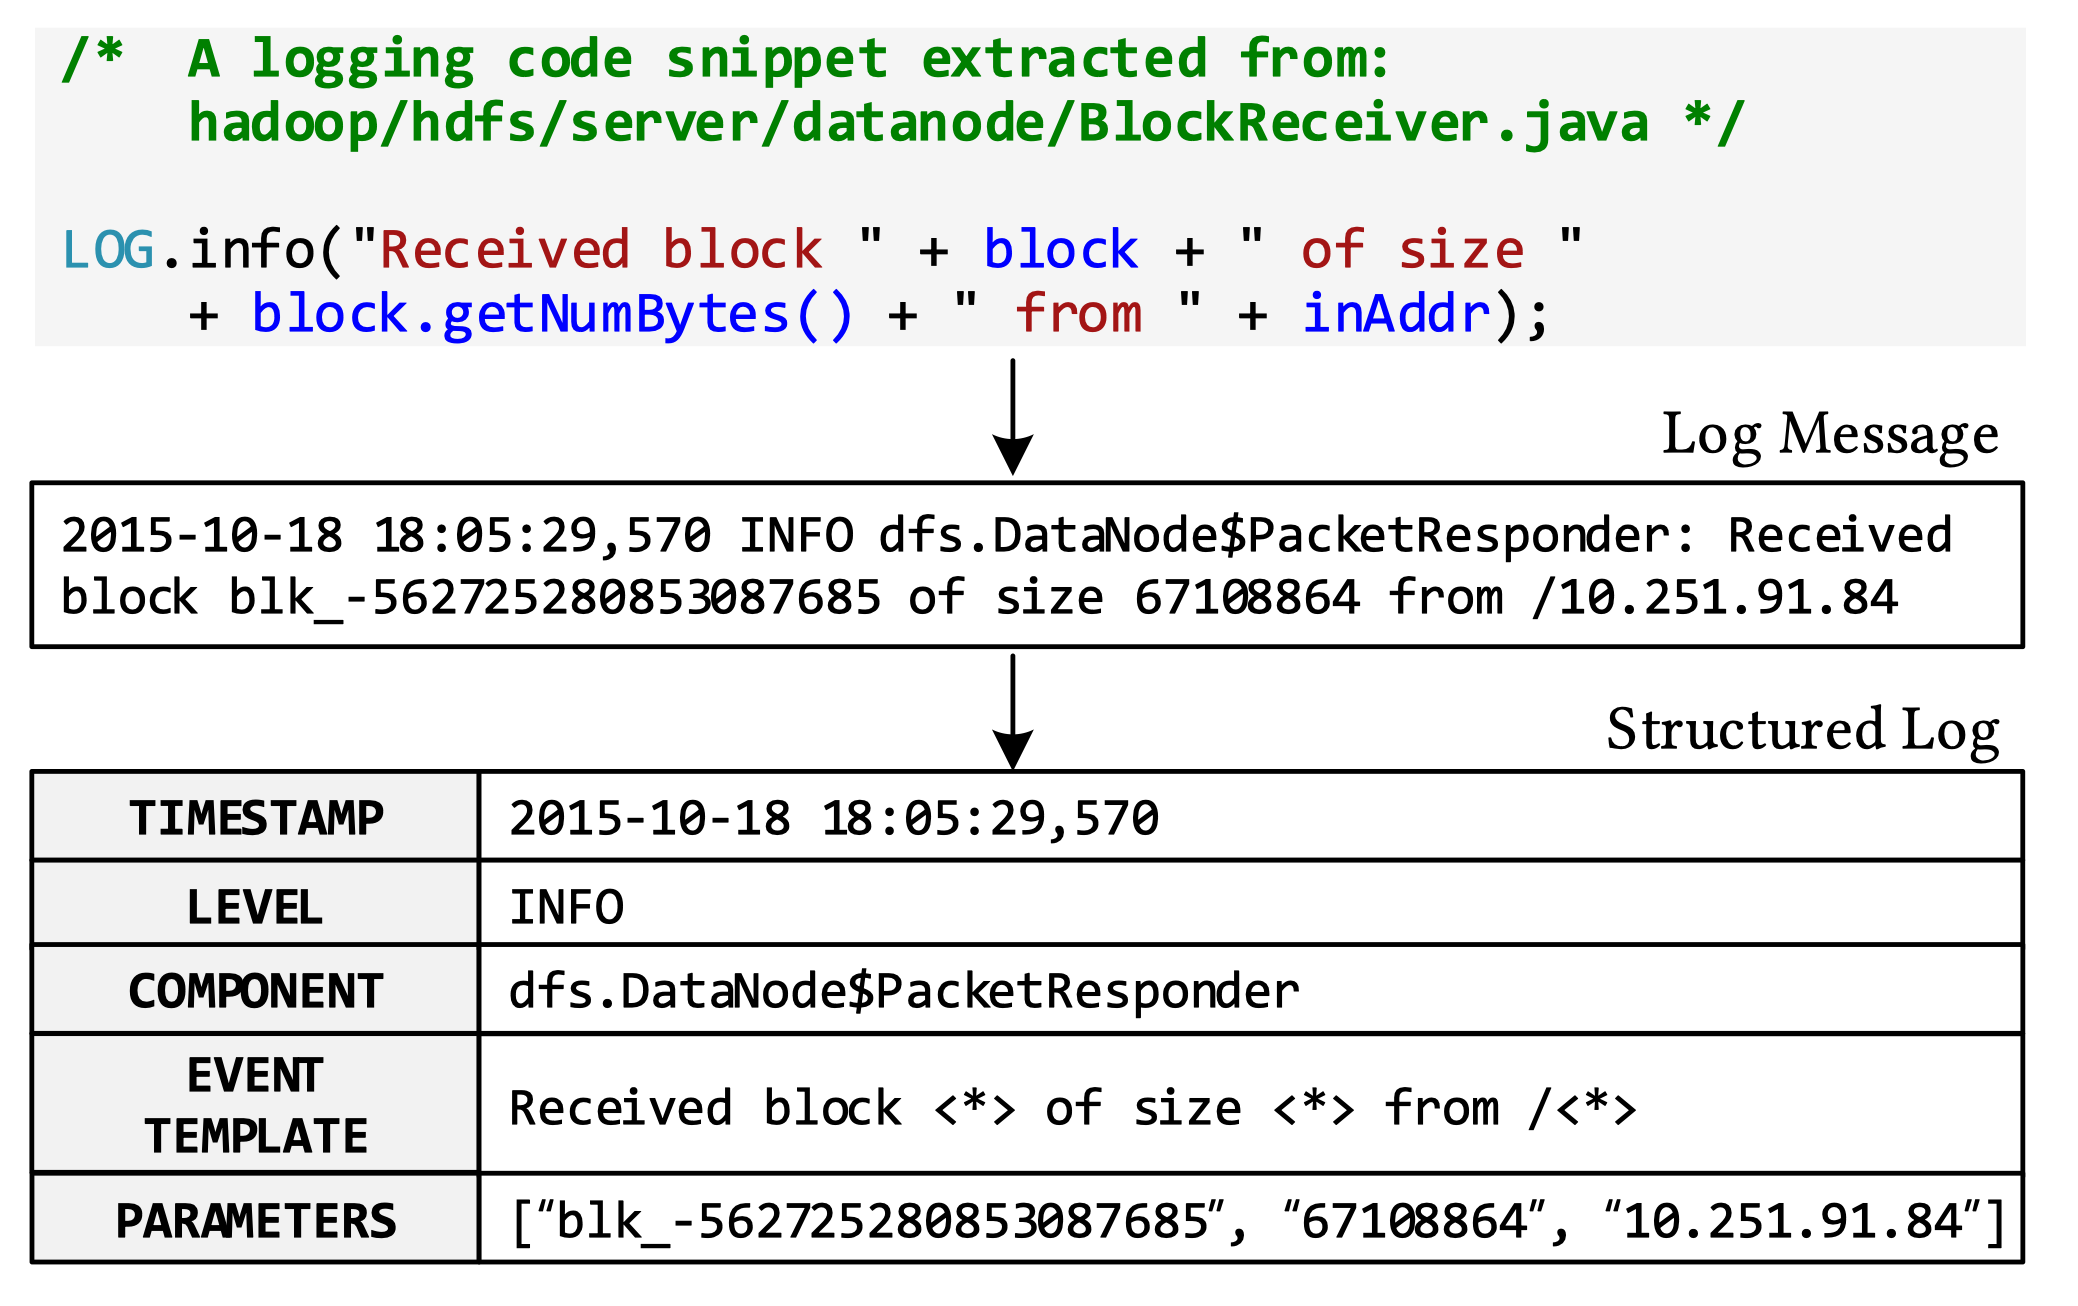
\includegraphics[width=12cm]{log_parsing.png}\\
  \caption{Schematic execution of log parsing \cite{zhu2019tools}}
  \label{fig:parsing}
\end{figure}


    \chapter{Concept \label{cha:concept}}
Establishing a connection between the latest advances in NLP and anomaly detection in system log data is a recently emerged field in research. The need for using language models to convert log events into word embeddings emerges from the weaknesses of older anomaly detection approaches that are not flexible enough to cope with the complex nature of system log data. There exist difficulties in reusing previously obtained knowledge from training on data from a given dataset and transferring it to a differently structured dataset. Most proposed techniques for solving the problem of anomaly detection in system log data suffer from not being transferable and being non-resilient to changing log data. The objective of this work is to provide a means to automatically detect anomalies in logs that are potentially affected by processing noise and changes of log events by updates of the underlying software, and to transfer knowledge obtained from a dataset of log sequences to another dataset of logs with a \textit{transfer of knowledge} method.

In section \ref{sec:problem_statement}, the general problem statement is defined, and necessary requirements for the model are specified. 
In the following section \ref{sec:overall_system}, the overall system architecture with its components is outlined and visualised.
In section \ref{sec:pre_processing} the necessary pre-processing steps for preparing the raw log messages for the anomaly prediction model are described in detail.
In section \ref{sec:prediction_model} the developed prediction approaches are described in detail. There exist two approaches, the regression and the classification approach, both using log event representations obtained by a language model.
In section \ref{sec:transferlearning} the transfer of knowledge mechanism is described.


\section{Problem Statement and Prerequisites \label{sec:problem_statement}}
Logs are print statements inside programs which are defined by a fixed sequence of code statements written by developers. The execution of a program is defined by these statements, and therefore follows a predetermined pattern. Hence, the produced logs must also follow certain patterns, chronological orders, and proportional relationships between number of occurrences of logs with each other.

\subsection{Formal problem definition \label{sec:formal_problem_definition}}
We define a system log $L$ as a sequence of log events or log messages $(m_0, m_1, ..., m_n)$ generated by logging instructions (e.g. \textit{printf()} or \textit{log.trace()}) within the software source code during the execution of the program. Log messages consist of a constant (log template) and a variable part.
Log messages consist of tokens - most tokens are English words, but do also include special characters. Each log message consists of a bounded sequence of tokens, $\mathbf{z_i}=(z_{j}\,:\,w \in  \mathbb{Z},\,j=1,2,...,|\mathbf{z_i}|)$, where $\mathbb{Z}$ is a set of all tokens, $j$ is the positional index of a token within the log message $m_i$, and $|\mathbf{z_i}|$ is the total number of tokens in $m_i$. For different $m_i$, $|\mathbf{z_i}|$ can vary. Depending on the concrete tokenisation method, $t$ can be a word, word piece, or character. Therefore, tokenisation is defined as a transformation function $\mathcal{T}: m_i \to \mathbf{t_i}, \forall i$.

We additionally introduce the notion a numerical vector representation (embedding vector). An embedding vector $e_i$ is a $d$-dimensional real valued vector representation of a log message template $t_i$. The embedding vector $e_i$ is obtained from a pre-trained language model $M(t_i)$.

\textit{Classification}: For every distinct log template $t_i$, we assign a class $c_i$. Let $g(E_i, \Psi): \left|s\right| \times \mathbb{R}^w \rightarrow \mathbb{R}^k,$ be a function computed by a neural network, that given a subsequence of $s$ vectors out of the dataset $E$, namely $E_i = (e_i, ..., e_{i+s})$, returns a probability distribution $Pr_i[e_{i+s+1}|E_i]$ = $(c_0: p_0, c_1: p_1, ..., c_k: p_k)$, describing the probability for each template class from $C$ to appear as the next class at index $i+s+1$, given $E_i$. The objective is to learn the parameters $\Psi$, so that for each fixed length sequence of vectors, the function predicts the correct set of possible subsequent classes. If one of the top $q$ candidate classes matches the actual class, then $\hat{b_i} = 0$ is returned, if none match the actual class, $\hat{b_i} = 1$ is returned.

\textit{Regression}: Let $h(E_i, \Phi): \left|s\right| \times \mathbb{R}^w \rightarrow \mathbb{R}^w$ be a function computed by a neural network, that based on a sequence of $s$ vectors $E_i = (e_i, ..., e_{i+s})$ predicts the vector $d$ at index $i+s+1$. The objective in this case is to learn parameters $\Phi$, so that the system predicts the vector following the sequence of vectors of length $s$. If the distance between the predicted vector $d$ and the actual vector $e_{i+s+1}$ is above or below threshold values, which will be computed by the q-th percentile of all loss values from the original dataset, then $\hat{b}_{i+s+1} = 1$ is returned, if it is inside these thresholds, then $\hat{b}_{i+s+1} = 0$ is returned.

\subsection{Requirements and Assumptions \label{sec:requirements_and_assumptions}}
\begin{enumerate}
	\item The model requires word vectors that are computed by a language model that has been pre-trained on a sufficiently large corpus.
	\item The model requires \textit{normal}, non-anomalous log data which do not contain anomalies for training.
	\item The model is not able to detect anomalies which are only detectable in the variable part of the log messages. The model only considers the templates, i.e. keys of the log message.
\end{enumerate}



\section{System Overview \label{sec:overall_system}}
In this section, a broad overview of the overall system is presented, with figure \ref{fig:overall_system} illustrating the steps necessary for the learning procedure, followed by anomaly prediction. 
The core concept can be outlined as follows: first, the original log sequences are ordered, then a log parser is used to extract templates $t_i$ from the original log sequences $(m_0, m_1, ..., m_n)$ and then transform the log sequences to template sequences $(t_0, t_1, ..., t_n)$. Afterwards, the template sequences are transformed into log sequence embeddings $(e_0, e_1, ..., e_n)$ by a language representation model $M$. This procedure is described in detail in section \ref{sec:pre_processing}.

For the training part, sub-sequences of log embeddings $E_i=(e_i,...,e_{i+s})$ are fed into a Bi-LSTM that learns to predict the next embedding $e_{i+s+1}$, which is called the regression task, specified in section \ref{sec:regression} and coloured red in figure \ref{fig:overall_system}. For the classification-based approach, the next template class $c_{i+s+1}$ is predicted, specified in section \ref{sec:classification} and coloured blue in figure \ref{fig:overall_system}. The results of these predictions are then compared to the true subsequent log embedding or class of the true subsequent log template, in order to train the model to identify non-anomalous log data.

The prediction part involves two steps: first, the template sequences obtained from the original log sequences A are altered by changing the order of the sequences or manipulating the templates, as described in section \ref{sec:logs_alteration}. As a second step, these manipulated sequences are fed to the model that has been trained on embedding sequences not containing any alterations, thereby obtaining the model's predictions $\hat{b}$.

Transfer of knowledge builds onto this process. After a model has been trained as described on dataset $A$, pre-processing is conducted the same way on a new dataset $B$, thus obtaining a sequences of embeddings. For the classification task, the template sequences of dataset $B$ are mapped to the class mappings of dataset $A$, and then used for prediction. The regression task functions analogously to learning without the transfer mechanism. Transfer of knowledge is described in detail in section \ref{sec:transferlearning}

\begin{figure}[h]
	\centering
	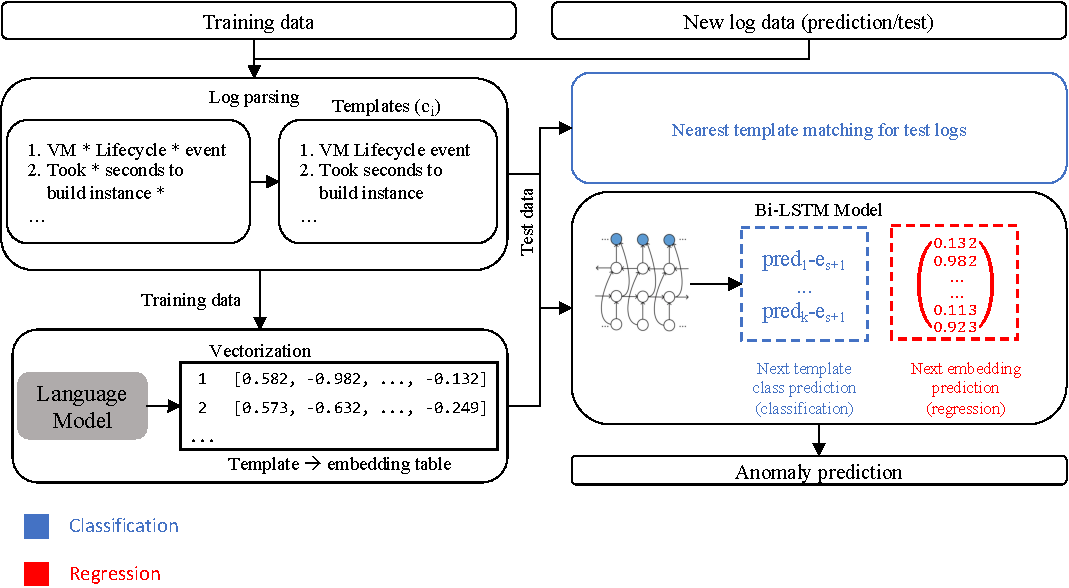
\includegraphics[width=1\columnwidth]{overview_new.pdf}
	\caption{Anomaly Detection System}
	\label{fig:overall_system}
\end{figure}

\newpage
\section{Pre processing \label{sec:pre_processing}}
Log files are usually available in an unordered, raw state, and need to be ordered, parsed and transformed into an appropriate format so that they can be handled as sequences by a Bi-LSTM. The required steps for this purpose are outlined in this section. In the first subsection \ref{sec:conceptlogparsing}, the steps required for parsing logs in order to obtain log templates $t_i$ are outlined, followed by the transformation into word embedding vectors $e_i$ in \ref{sec:word_vectorization}. A diagram illustrating the complete pre-processing pipeline can be see in figure \ref{fig:full_preprocessing_pipeline}.

\subsection{Log Parsing}\label{sec:conceptlogparsing}
Log parsing is an important step for automated anomaly detection, as already described in section \ref{sec:backgroundlogparsing}, since raw log messages are unstructured data and contain a lot of extra information. 
For this work, the log parser Drain \cite{he2017drain} is utilised. It is characterised by high accuracy and efficiency \cite{he2017drain} and achieves the best results compared with other related methods, evaluated in \cite{zhu2019tools}. The detailed result of the execution of a log parser can be see in figure \ref{fig:parsing}. 
There are a few important aspects to note: Not only does the log parsing step extract log templates, but it also extracts other valuable information in a structured way, namely timestamps and, in this example the bulk id. Timestamps are needed, in order to make sure that the logs are in the correct chronological order, since it is possible, that system logs are an aggregation of log output of different sub-routines or different instances, which can happen concurrently, thus producing unordered logs. Additionally to sorting by timestamps, it can also be required to sort system logs by group ids, instance ids or bulk ids as it can be seen in step 1) in figure \ref{fig:full_preprocessing_pipeline}. Matching instance ids are identified, made visible by marking same instance ids yellow. They are then separated in order to be able to observe each self-contained block separately from other blocks. After these sorting procedures, the result of the log parser's transformation $\mathcal{T}: m_i \to \mathbf{t_i}, \forall i$ from log messages to templates are visible as step 2) in figure \ref{fig:full_preprocessing_pipeline}.

\subsection{Template cleansing \label{sec:template_cleansing}}
Even though log parsing and the aforementioned ordering steps largely improve the further processability of logs for sequential learning, by making it possible to single out the fundamental semantics of a log event, they are still partly made up of special characters and variable names. The following characters are removed:
\begin{enumerate}
	\item All non-character tokens such as delimiters, digits, and particularly variable placeholders (\verb!<*>!).
	\item All concatenations of words are split, for example \verb!sync_power_state! will be split into the separate words \verb!sync!, \verb!power! and \verb!state!
	\item All leading, trailing and repeated whitespace characters are removed.
\end{enumerate}

This part of the pre-processing is marked with step 3) in figure \ref{fig:full_preprocessing_pipeline}.

\subsection{Word vectorisation \label{sec:word_vectorization}}
After the aforementioned pre-processing steps, the log events are transformed into word embeddings, using a language model that is able to convert words or whole sentences into word or sentence embedding, effectively representing function $M(t_i)$ defined in \ref{sec:formal_problem_definition}. The process of transforming a sequences of logs with the API of a language model is visualised in figure \ref{fig:transform_sequence_to_embeddings}.

Satisfying the following two requirements is essential in the context of providing suitable word embeddings for the anomaly detection task:
\begin{itemize}
	\item Distinguishability: Word embeddings should capture the difference between log events with differing semantics. For example ``\verb!<*> Terminating instance!" and ``\verb!<*> Deleting instance files <*>!" are log events with highly different semantics, even though they contain equal (instance) and in the broader sense similar (terminating, deleting) words. This means their cosine distance should be high.
	\item Tolerance: Word embeddings should capture the similarity between different log events with same or very similar semantics. For example, the log event pair ``\verb!<*>! \verb!Creating image!" and ``\verb!<*> Image created successfully!" or ``\verb!VM up!" and \\ ``\verb!VM started!". This in turn should result in a low cosine distance \cite{zhang2019robust}.
\end{itemize}

In oder to be able to compare the quality of different language model's word embeddings with regards to the task of anomaly detection, it is possible to easily swap the used language model for log event transformation. For this work, the pre-trained language models used for evaluation are Bert, GPT-2 and XL-Transformers. 


\begin{figure}[H]
	\centering
	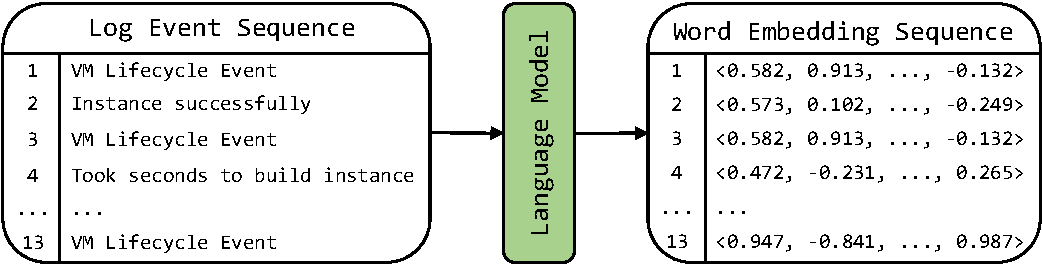
\includegraphics[width=1\columnwidth]{transform_templates_to_embeddings.pdf}
	\caption{Transformation of a log event sequence to a word embeddings sequence.}
	\label{fig:transform_sequence_to_embeddings}
\end{figure}



\subsection{Finetuning\label{sec:finetuning}}
Word embeddings models are usually provided pre-trained in different formats (e.g. with or without upper case), because training them from scratch is expensive - for Bert, it requires 4 days of training on 16 cloud TPUs for one language \cite{googlebert}. They are trained on large corpuses with unsupervised tasks. In order to make them more useful with regards to the task of anomaly detection, it is reasonable, to adjust the given pre-trained datasets using the log data corpora, by using the finetuning API provided by the language models. For this purpose, the log corpus on which finetuning shall be executed is prepared for the finetuning task of Masked Language Model, as described in subsection \ref{Bert}.

\subsection{Log Alteration\label{sec:logs_alteration}}
By altering log events the evolution and instability of log events is being simulated. Since software is changed by developers, also log statements are subject to constant change. It is therefore necessary to build a flexible model that does not have to be retrained completely after each update of a log producing software. Log alteration is also used to simulate a different dataset $B$ based on a given dataset $A$, for the evaluation of the model on drastically changed logs that appear like from another dataset, as outlined in \ref{sec:transferlearning}.

Anomalies and alterations can be injected at arbitrary ratios. Various types of alterations are injected into original log data, either on the log event itself as depicted in figure \ref{fig:changelogevent} or on the sequence of log events as visualised in figure \ref{fig:changesequence}.

Three types of alterations are injected into the log events: a various amount of words is inserted between the tokens, for example words that appear in the context of logs, like ``\textit{deleted}", ``\textit{during}", ``\textit{for}" or ``\textit{time}". Words can also be also deleted or replaced. It is not expected that the system detects a log event as an anomaly, that has not been changed much, i.e. only one word has been added into a statement (e.g. if ``\textit{* Took *.* seconds to deallocate network for instance.}" has been changed to ``\textit{* Took *.* seconds to deallocate network for \textcolor{red}{this} instance.}").

Additionally, it is possible to perform changes on the sequence of logs. In the following example, let $M = (m_i : i = 0, 1, 2, ..., n))$ be a sequence of log events:
\begin{itemize}
	\setlength\itemsep{-0.5em}
	\item events can be \textit{deleted} from the sequence, meaning that if the event at index $j$ is selected for deletion, the resulting sequence is $M_{del} = (m_0, ..., m_{j-1}, m_{j+1}, m_n)$.
	\item events can be \textit{shuffled}, meaning that if the event index $j$ is selected for shuffling at index $k$, the resulting sequence is $M_s = (m_0, ..., m_j, m_k, m_{k+1}, ..., m_{j-1}, m_{j+1}, ..., m_n)$
	\item events can be \textit{duplicated}, meaning that if the event at index $j$ is selected for duplication, the resulting sequence is $M_{dup} = (m_0, ..., m_j, m_j, m_{j+1}, ..., m_n)$
	%\item new events can be \textit{inserted} meaning that if the event $m_{new}$ is inserted at index $j$, the resulting sequence is $M_{ins} = (m_0, ..., m_{new}, m_j, m_{j+1}, ..., m_n)$
\end{itemize}

Similar to the insertion of minimal alterations on the log events themselves, it is expected of the system not to detect an anomaly for the deletion, duplication or shuffling of events, since these also can reflect minor changes through new valid execution paths due to version updates and new deployments.
\vfill

\begin{figure}[H]
	\centering
	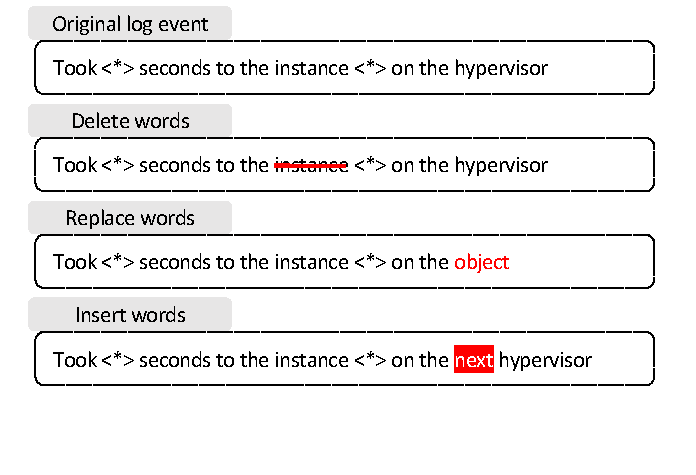
\includegraphics[width=11cm, height=7.5cm]{change_log_event.pdf}
	\caption{Altering log events.}
	\label{fig:changelogevent}
\end{figure}

\begin{figure}[H]
	\centering
	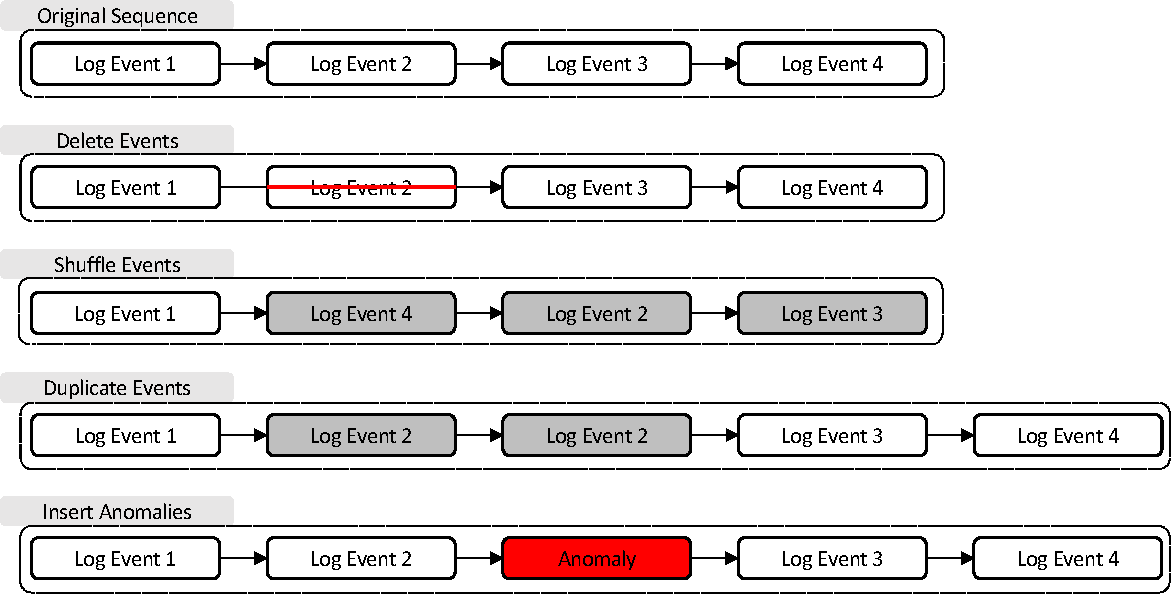
\includegraphics[width=14cm,height=6.8cm]{change_sequences.pdf}
	\caption{Altering log sequences.}
	\label{fig:changesequence}
\end{figure}

\begin{comment}
\begin{figure}[!tbp]
  \centering
  \subfloat[Altering log events.]{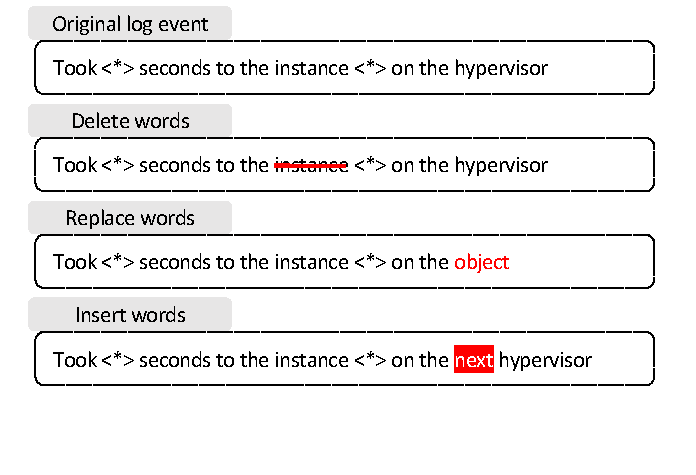
\includegraphics[width=0.3\textwidth]{change_log_event.pdf}\label{fig:changelogevent}}
  \hfill
  \subfloat[Altering log sequences.]{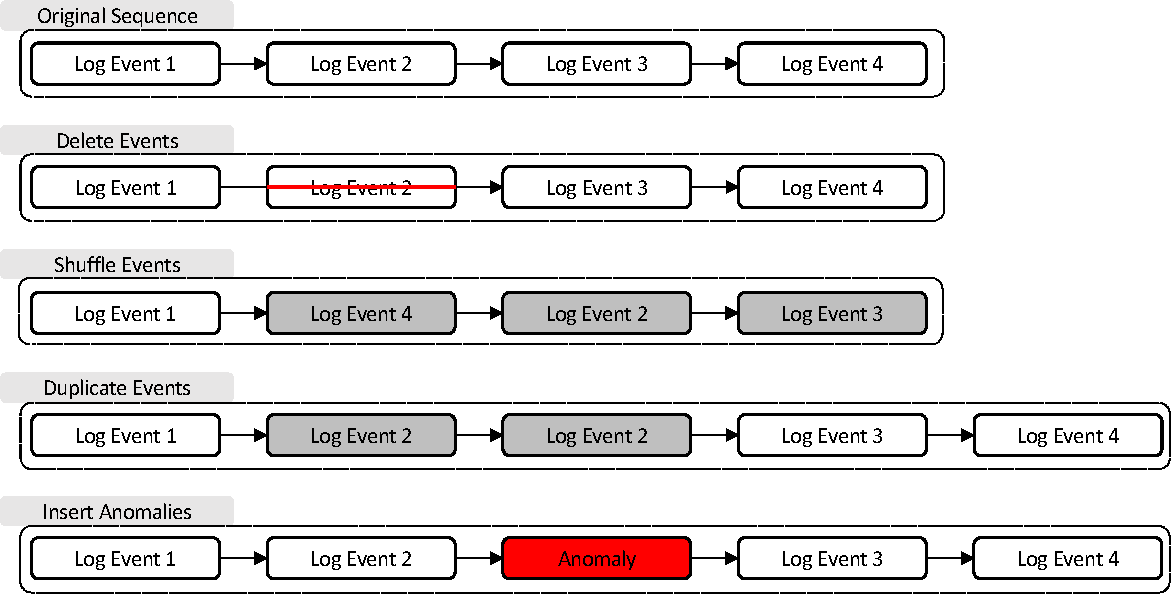
\includegraphics[width=0.65\textwidth]{change_sequences.pdf}\label{fig:changesequence}}
  \caption{Alteration of log events and sequences.}
\end{figure}
\end{comment}


\section{Prediction Model\label{sec:prediction_model}}

\subsection{LSTM Model\label{sec:lstm-model}}
Through the aforementioned steps in \ref{sec:pre_processing}, the system log $L$ has been transformed into a sequence of word embeddings $e_i \in \mathbb{R}^w$. In order to learn sequences of logs, a sequence of $s$ log embeddings are concatenated to form an embedding sequence $E_i = (e_i,...,e_{i+s})$. Taking a sequence of embeddings as input, a \textit{Bi-LSTM} neural network as described in \ref{sec:bi-lstm} is utilised to predict the class or embedding at position $i+s+1$. Figure \ref{fig:lstm_model} shows the structure of the Bi-LSTM. As a first step a dropout layer is applied to the input sequence which randomly drops out information in order to reduce overfitting and improve generalisation, before feeding it to the forward and backward layers of the Bi-LSTM. This way, more information of the input log sequences can be captured than when only an uni-directional LSTM would be utilised. Then, the outputs of the Bi-LSTM are again fed into a dropout layer, followed by a fully connected layer which reduces the output of the LSTM to the desired dimensions, i.e. $\mathbb{R}^w$ for regression and number of classes $c$ for classification. Finally, an activation function $act$ is applied to the last output $o_{i+s+1}$, \textit{log-softmax} for classification and \textit{linear} for regression, respectively, in order to obtain the model's prediction $p_{i+s+1}$.


\begin{figure}[H]
	\centering	
	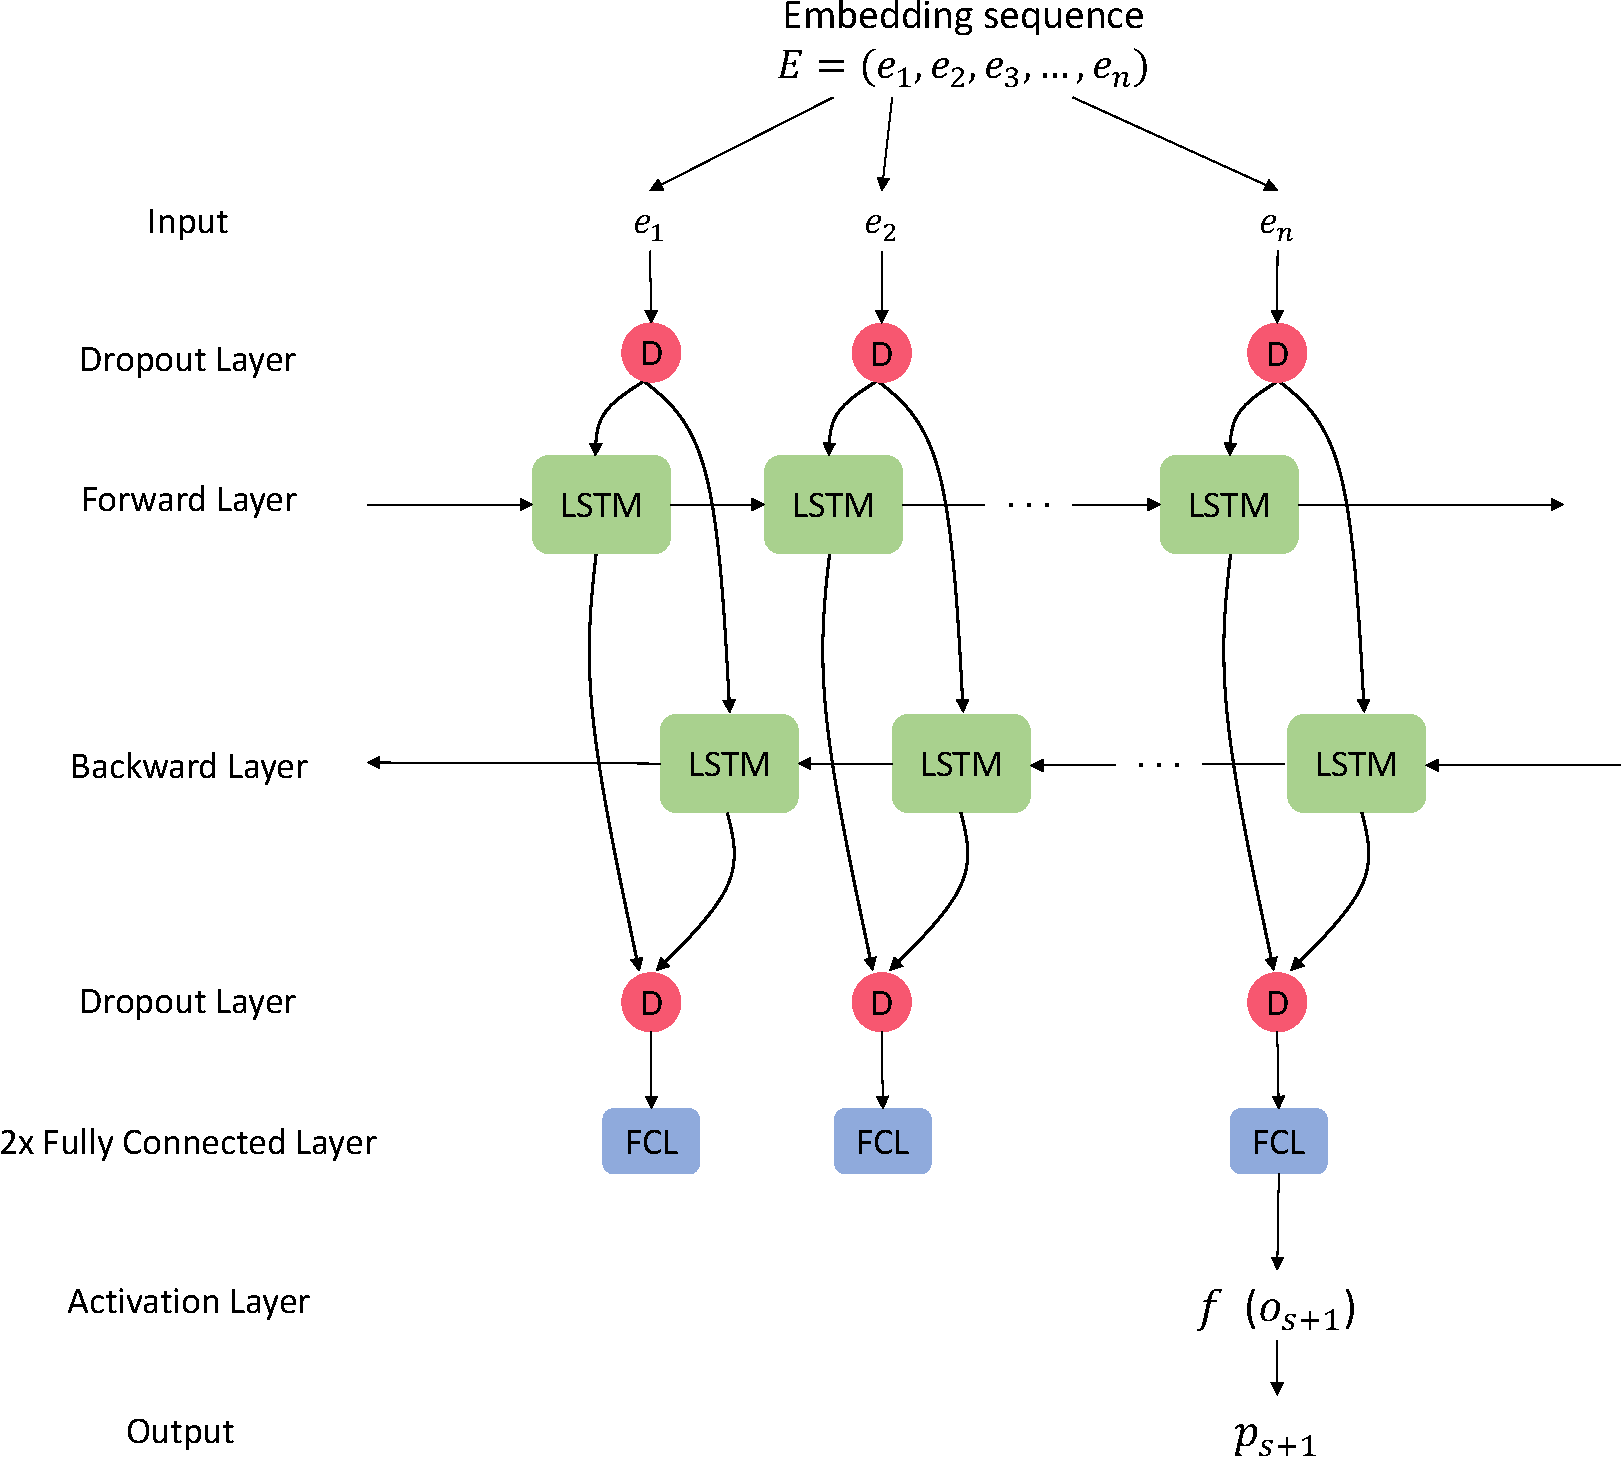
\includegraphics[width=16cm]{lstm_model.pdf}
	\caption{Bi-LSTM model}
	\label{fig:lstm_model}
\end{figure}
\newpage
\subsection{Classification \label{sec:classification}}
For the classification approach, the finite set of $n$ unique log event templates is mapped to class indices $c_0, ..., c_n$. Training of the neural network is then performed on original log data that does not contain anomalies.
\begin{itemize}
\setlength\itemsep{-0.5em}
	\item The \textit{input} values of the training data have the dimensions $n$, $s$ and $w$, with $n$ being the number of unique log events, $s$ being the length of the sequence of word embeddings for which the neural network shall learn the consequent class and $w$ being the dimensionality of the log event embeddings.
	\item The \textit{target} values of the training data are structured as follows: for every sequence of word embeddings $E_i = (i, ..., i+s)$, there is a corresponding class $c_{s+i+1}$ that stands for the template at position $s+i+1$. The system is trained to predict that class correctly.
\end{itemize}

After training has been executed on the \textit{train} dataset, the prediction phase starts, where a \textit{test} dataset containing anomalies and alterations, as described in \ref{sec:logs_alteration}, can be processed by the neural network. For a new incoming test dataset, the system first has to match every template to the template classes of the train dataset. For every template in the test dataset, the nearest neighbour out of the templates of the train dataset is determined and will get the respective class assigned, as depicted in figure \ref{fig:label_mapping}. This means in particular, that for every unique template, the corresponding word embedding is retrieved, and then every one of the word embeddings of the test dataset is mapped to the word embedding from the train dataset with the lowest cosine distance. Additionally, a threshold has to be found, so that if for a given embedding in the test data, no corresponding embedding with a cosine distance below this threshold is found, that template shall not get a class assigned, this would otherwise lead to a situation where the log event gets mapped to any of the template classes, which is not wanted behaviour.

After the matching process is finished, the system can read in the sequences of log events of the test data. For every sequence of log events $E_i$ of length $s$, the system returns a probability distribution $Pr[c_{s+i+1}|E_i] = \{c_0 : p_o, c_1 : p_1, ..., c_n : p_n\}$ that denotes the probability of each log template class to appear as the subsequent one. It is possible, that there are multiple candidates for the following template. Let's assume, that the system is attempting to terminate an instance, then the corresponding template to class $c_{s+i+1}$ could be for example '\textit{Instance terminated successfully}' or '\textit{Waiting for instance to terminate}'. The possible template classes $c_i$ are sorted based on their probabilities. A predicted template class is considered normal, resulting in the system's prediction $\hat{b}_{s+i+1}=0$, if it is among the top $q$ candidates. It is marked as anomalous, $\hat{b}_{s+i+1}=1$ otherwise.
 

\begin{figure}[H]
	\centering
	\captionsetup{justification=centering}
	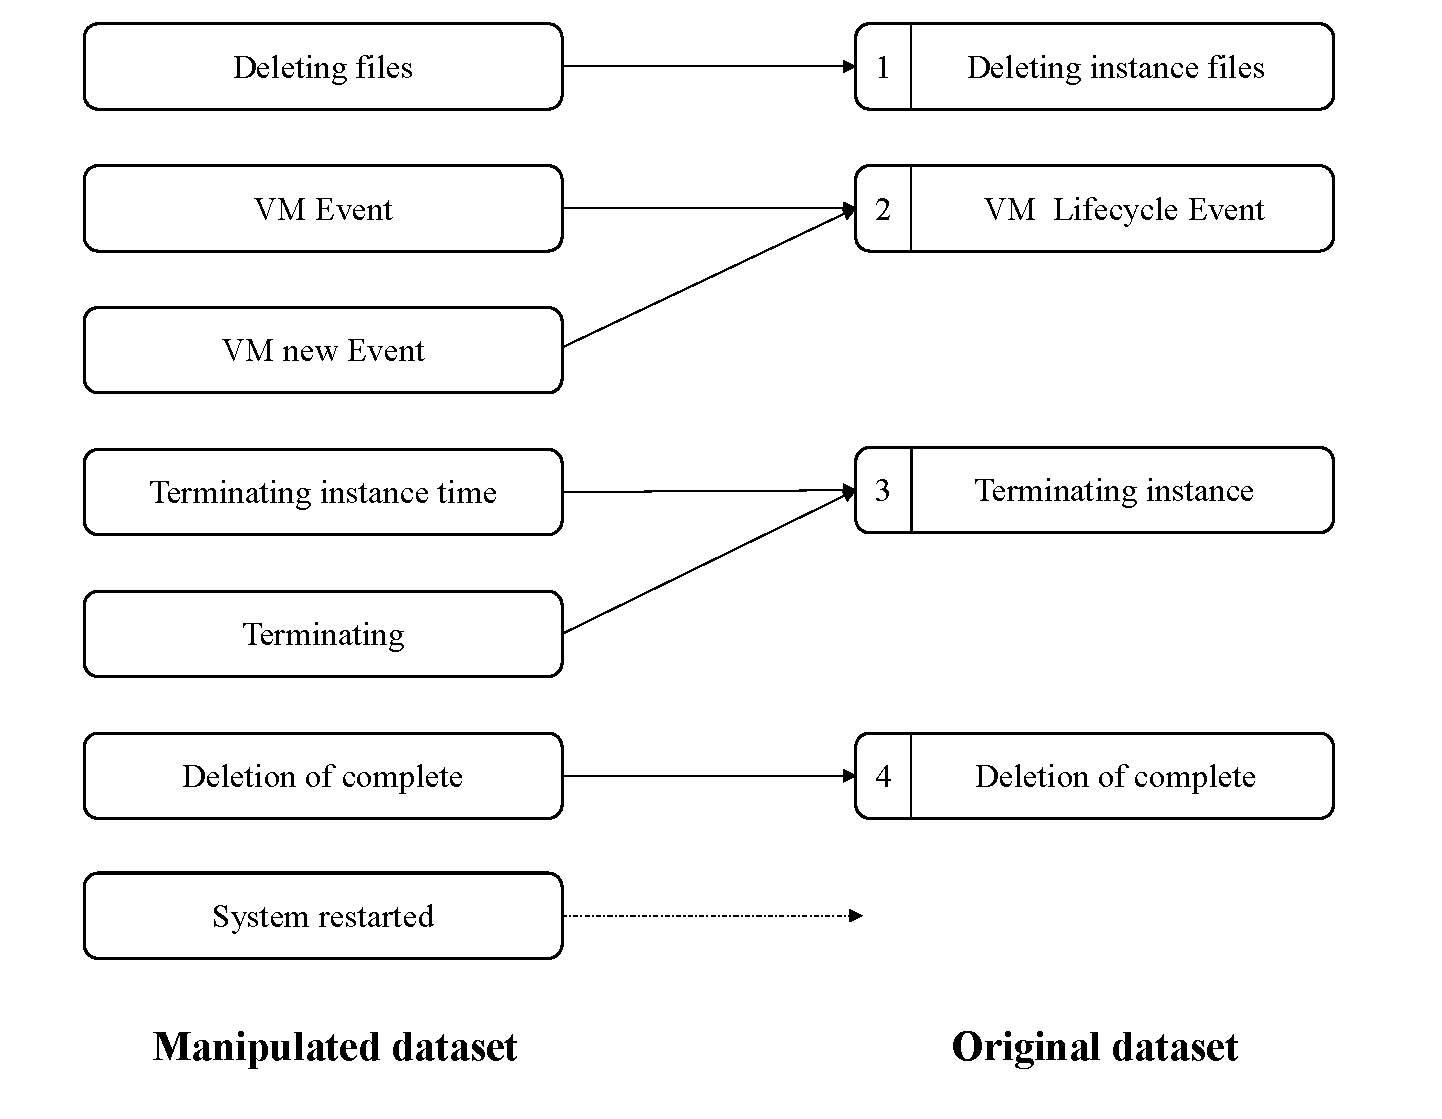
\includegraphics[width=15cm]{label_mapping.pdf}
	\caption{Template mapping}
	\label{fig:label_mapping}
\end{figure}

\begin{figure}[H]
	\centering	
	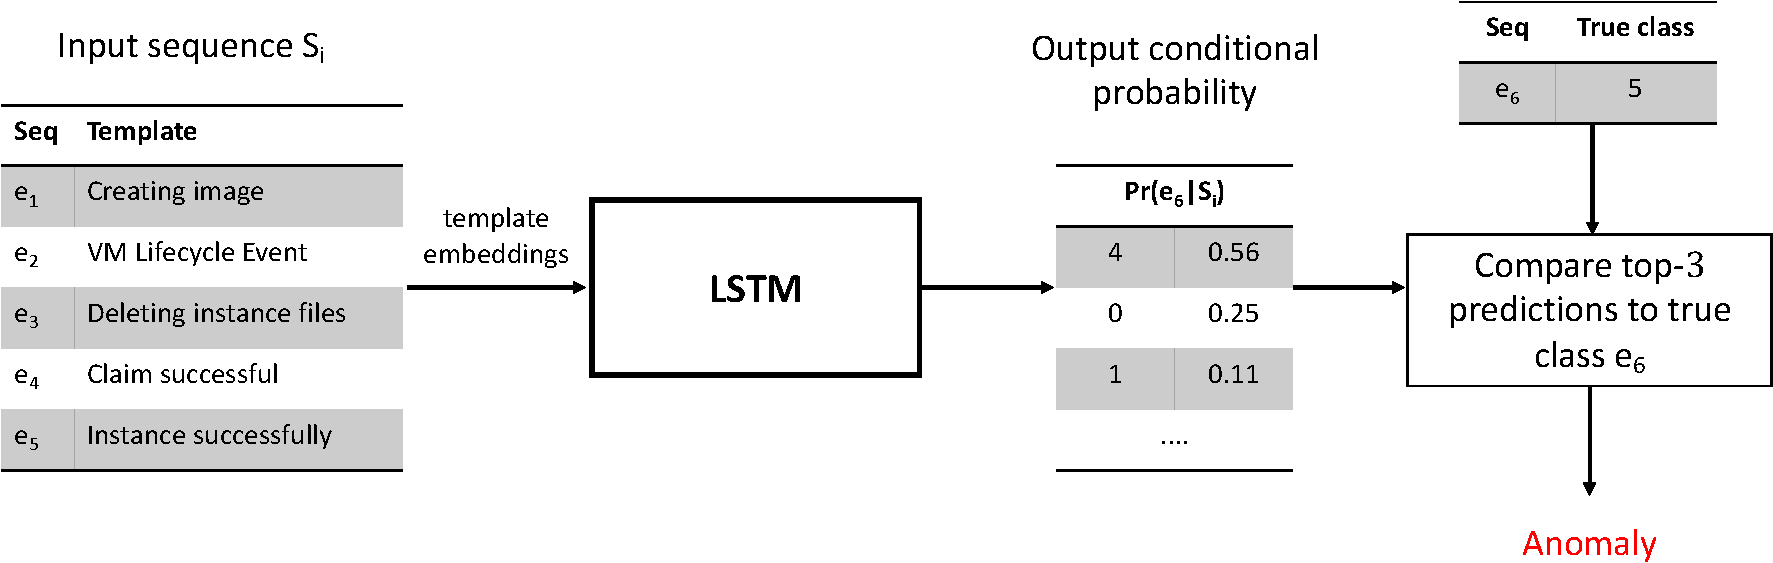
\includegraphics[width=15cm]{classification_detect.pdf}
	\caption{Class Prediction example for $g=3$}
	\label{fig:class_prediction}
\end{figure}
\newpage
\subsection{Regression \label{sec:regression}}
For the regression approach, the neural network is trained to solve a regression task, with the input values of the training data being structured as described in \ref{sec:classification}, while the corresponding target value for the sequence of embeddings $E_i = (e_i, ..., e_{i+s})$ is the embedding of the log event at position $i+s+1$, meaning the neural network shall predict the next embedding $e_{i+s+1}$. After training on the original dataset, the mean squared error loss of every target word vector at position $i+s+1$ of the corresponding input sequence $E_i$, and the neural network's predicted word vector, is computed. Afterwards, the \textit{q-th} percentile of the agglomerated loss values of the original dataset is computed. The optimal value \textit{q} for the following purpose is to be determined by performing a grid-search. For the sequences of the test dataset, the loss values are computed in the same way as for the original dataset. This is depicted in figure \ref{fig:regression_with_threshold}. The system will then mark every log event at position $i$ whose word embedding's loss value is above the calculated \textit{q-th} percentile as an anomaly, with $\hat{b}_i=1$, otherwise as non anomalous, with $\hat{b}_i=0$.

\begin{figure}[h]
  \centering
  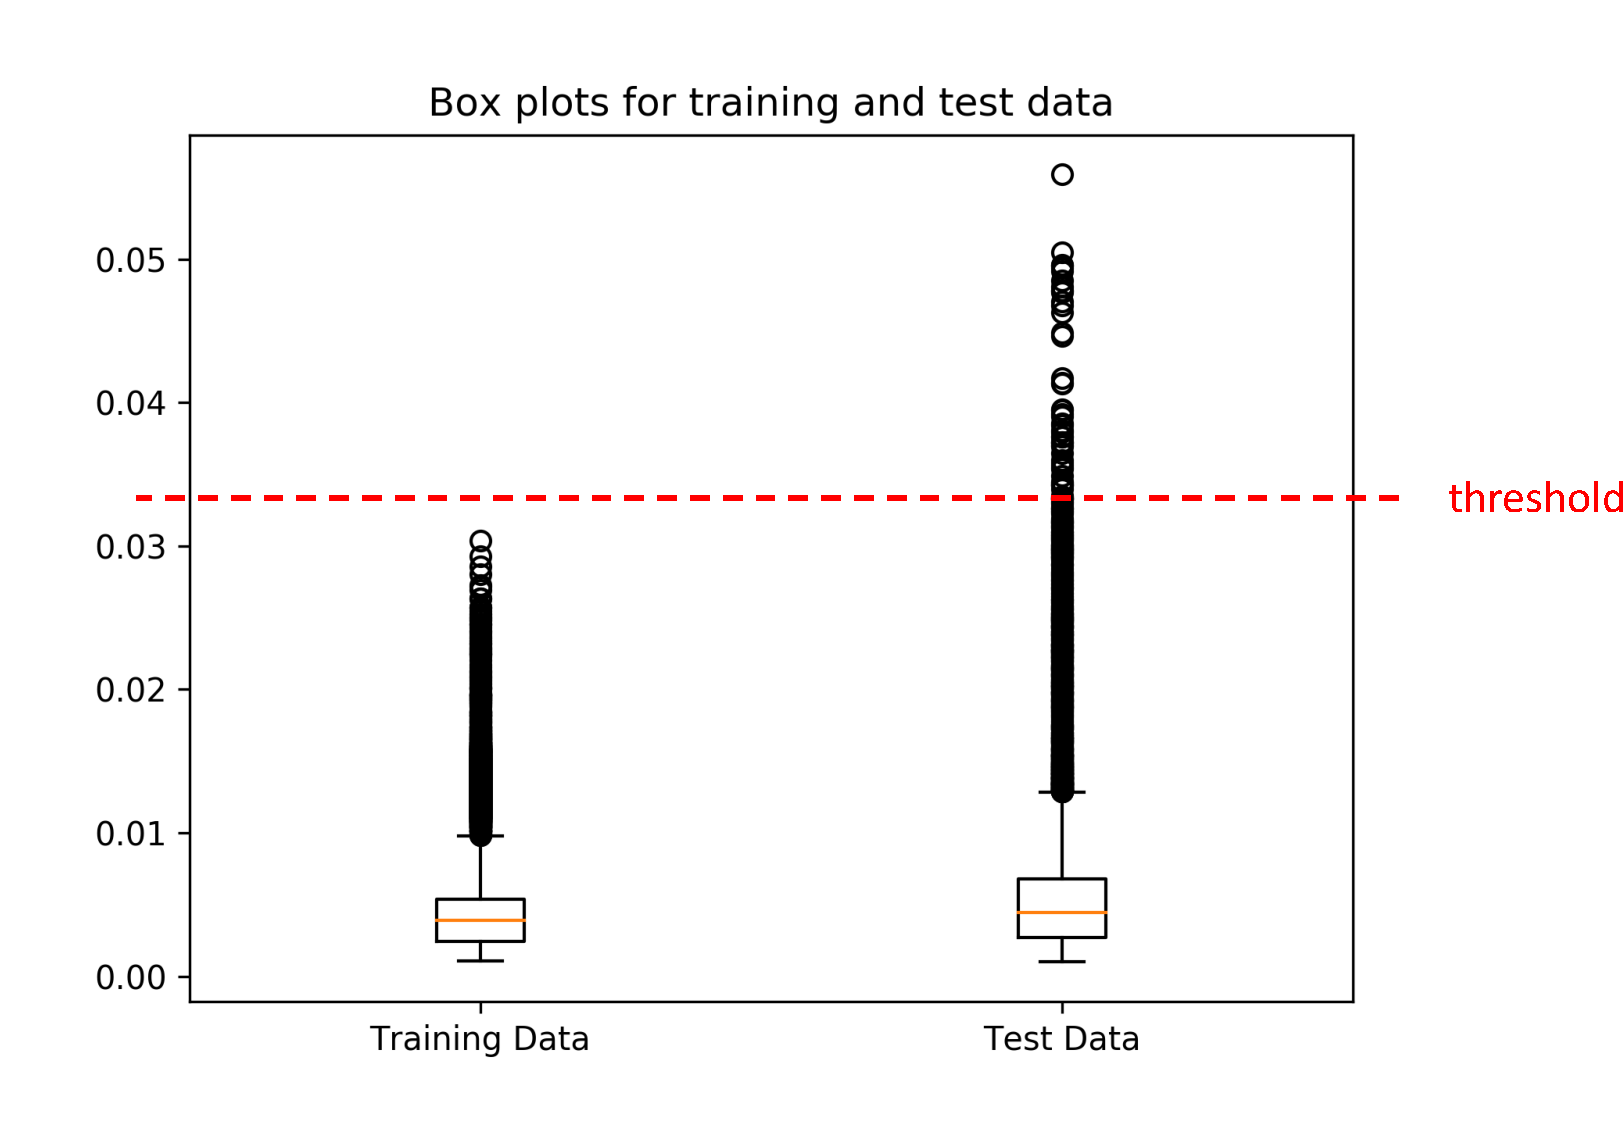
\includegraphics[width=15cm]{regression_box_plots_example.pdf} \\
  \caption{Box plots showing the distribution of loss values for training and test data.}
  \label{fig:regression_with_threshold}
\end{figure}

\newpage
\section{Transfer of Knowledge \label{sec:transferlearning}}
As already mentioned in chapter \ref{cha:introduction}, modern cloud systems and their underlying software are subject to constant change. Through continuous re-deployment and updates of services and systems, there is a lack of sufficient data to perform training of a new anomaly detection model. Therefore, using pre-trained general purpose language models for extracting vector representations of logs and re-usage of already pre-initialised weights of a Bi-LSTM model from training on older log version allows transferring the model to new unseen logs. Let dataset $A$ be the training dataset from already known log messages, and dataset $B$ be a log dataset from an updated version of the system. The steps for prediction of unseen logs using the classification approach are outlined in subsection \ref{sec:transfer_classification} and for the regression approach in subsection \ref{sec:transfer_regression}.

\begin{comment}
\begin{figure}[H]
	\centering
	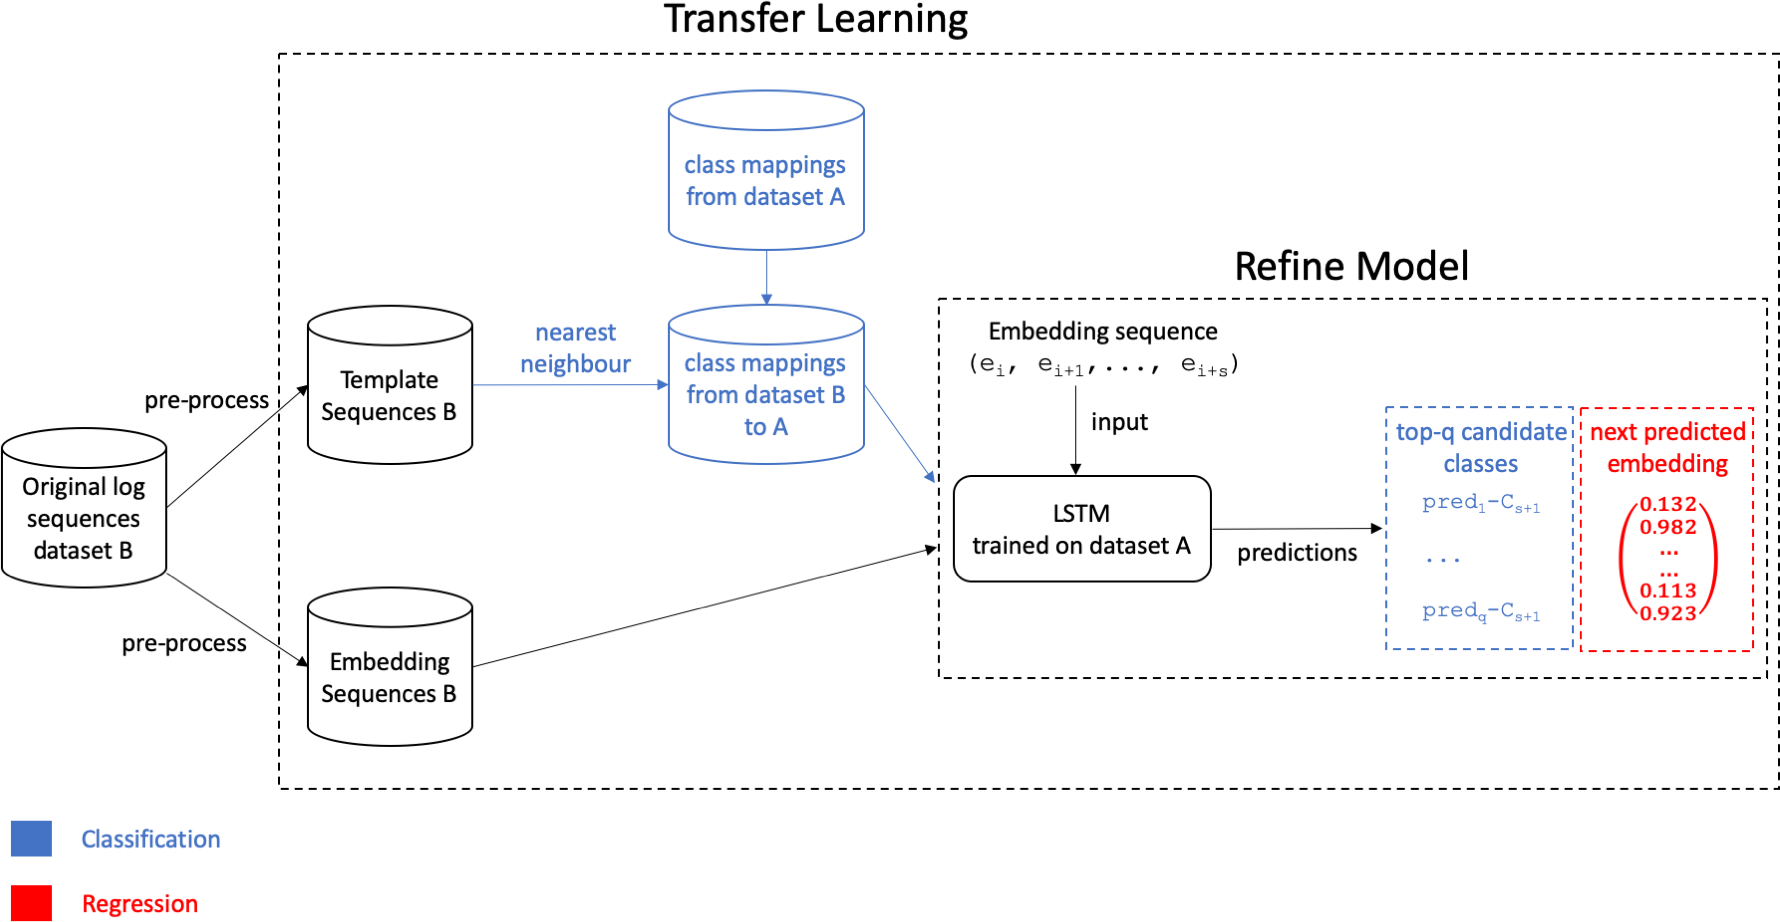
\includegraphics[width=15cm]{transfer-learning.png}
	\caption{Transfer of Knowledge System}
	\label{fig:transfer_learning_system}
\end{figure}
\end{comment}

\subsection{Classification \label{sec:transfer_classification}}
For the classification approach, the model is first trained as depicted in the pre-processing and training part of figure \ref{fig:overall_system} on a train dataset $A$. Then, in order to re-use the trained model, several preliminary steps are executed. First, every log event of a training dataset $B$ is mapped to the nearest neighbour of train dataset $A$, i.e. the word embedding with the shortest cosine distance, and gets assigned the same class. This is the same procedure as described in \ref{sec:classification} and depicted in \ref{fig:label_mapping}, with the only difference that there does not exist a threshold for assigning a class. Every log event will get a class assigned. Then, few-shot training on the training dataset $B$ will be executed, in order to adjust the model to the new dataset $B$. As a final step, with the adjusted model on training dataset $B$, the prediction phase on a test dataset $B$ can be executed, completely analogous to the description in \ref{sec:classification} and as depicted in \ref{fig:overall_system}.

\subsection{Regression \label{sec:transfer_regression}}
For transfer of knowledge using the regression-based approach, the model is first trained as depicted in the pre-processing and training part of figure \ref{fig:overall_system} on a train dataset $A$. Then, the same weights of the LSTM that have been learned from this training are re-loaded, and few-shot training on a different train dataset $B$ is executed. The model is then ready to make predictions on anomalies on a test dataset $B$ using the approach described in \ref{sec:regression}.



\begin{figure}[htb]
  \centering
  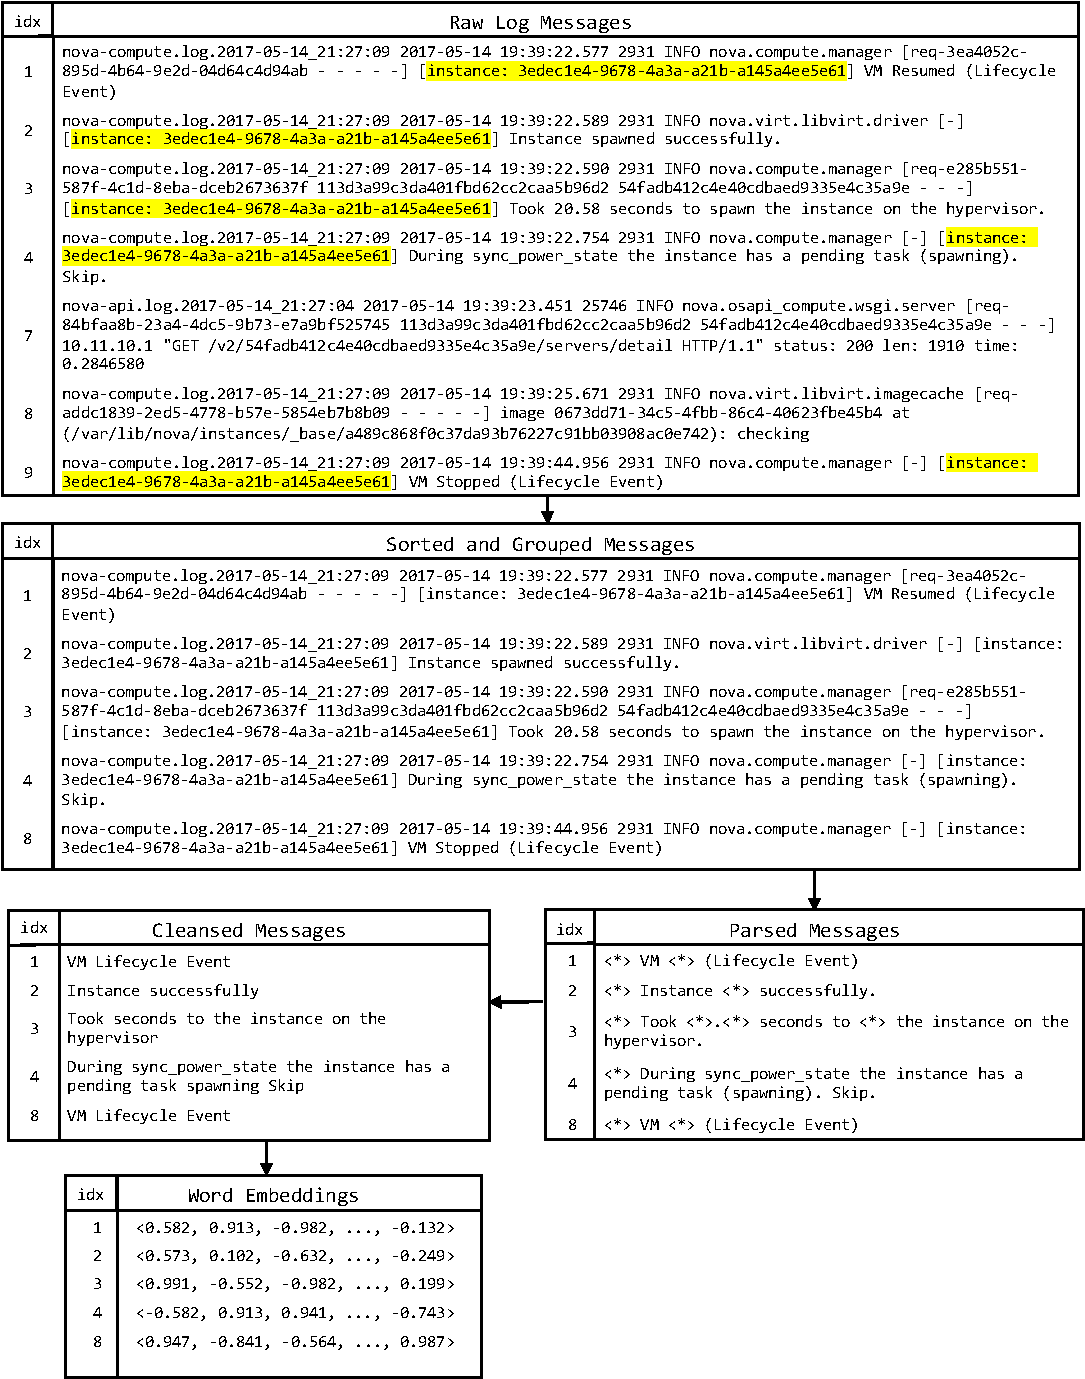
\includegraphics[width=15cm]{parsing_full.pdf}\\
  \caption{One full iteration of the pre-processing pipeline.}
  \label{fig:full_preprocessing_pipeline}
\end{figure}








    \chapter{Results\label{cha:results}}

In the following chapter, the achieved results of the model are presented. The described approaches are evaluated with regards to the common metrics precision, recall, and F1-Score. Different hyperparameter-setups are discussed and visualised in graphs. In particular, the language models Bert, XL-Transformers and GPT-2 as described in \ref{sec:word_vectorization} are compared. Additionally, the regression-based method as described in \ref{sec:regression} and the classification method as described in \ref{sec:classification} are compared, showing advantages or disadvantages among each other.

In section \ref{sec:experimental_setup} details about the used hardware and technologies are listed, followed by section \ref{sec:evaluation} in which the results of the evaluation are presented. Finally, in section \ref{sec:discussion_results} the results of the evaluation are discussed.


\section{Experimental Setup\label{sec:experimental_setup}}
In this section, the used hardware, libraries, the dimensions of the word embeddings for every language model and the used log dataset are described.

\subsection{Hardware and Library Specifications}
The machine that was used to conduct the experiments has the following specifications:
\begin{itemize}
	\item Intel(R) Core(TM) i5-9600K CPU @ 3.70GHz
	\item 128 GB RAM
	\item 2 x NVIDIA GeForce RTX 2080 Ti 11GB RAM
	\item Ubuntu 18.04.3 LTS
\end{itemize}

\noindent The most relevant libraries that were used are:
\begin{itemize}
	\item Python 3.6.7
	\item Numpy 1.14.5
	\item PyTorch 1.4.0
	\item Transformers 2.3.0
	\item Tensorflow 2.1.0
\end{itemize}

\noindent The word embedding vector of the used language models have the following dimensions:
\begin{itemize}
	\item Bert: 768 
	\item GPT-2: 768
	\item XL-Transformers: 1024
\end{itemize}

\subsection{Anomaly Detection on one Dataset \label{sec:ad_one_ds_result}}
For evaluating the model, the OpenStack datasets "normal log dataset 2" (referenced to as original dataset from now on) containing 137k log lines and the "log dataset having performance anomalies" containing 18k log lines (referenced to as test dataset from now on), provided by the DeepLog authors at the University of Utah are used \cite{utah_dataset}. The original dataset stems from logs from running multiple OpenStack instances for 20 hours and 13 minutes for the original dataset and 2 hours and 17 minutes for the test dataset on CloudLab \cite{cloudlab}. Since the test dataset contains anomalies which are only detectable by inspecting the parameters of the log events, as described in \ref{fig:parsing}, i.e. the variable part of the log event which is not visible in the template after parsing, a total of 5\% of anomalies in relation to the total number of lines of the test dataset are injected into the test dataset, yielding a labeled test dataset for evaluation of the trained model. This is necessary due to the assumptions specified in \ref{sec:requirements_and_assumptions}. Table \ref{tab:test_train_ds} gives an overview of the amount of log lines per dataset. The number of \textit{raw lines} reflects the number of log lines in the dataset's initial state, while the number of \textit{lines ordered} specifies the number of log lines after 
In order to assess the quality of the used word embeddings, log alterations are additionally injected into the dataset containing anomalies, in order to simulate the instability of logs as described in \ref{sec:logs_alteration}.

\begin{table}[ht]
\centering
\begin{small}
\begin{tabular}{ p{1.3cm} p{1.8cm} p{2.3cm} p{1.7cm}}
\toprule
Dataset & \#lines raw & \#lines ordered & Anomalies\\
\midrule
Train & 137k & 33k & 0\%\\
Test & 18k & 5k & 5\%\\ 

\bottomrule
\end{tabular}
\caption{Test and train dataset.}
\label{tab:test_train_ds}
\end{small}
\end{table}


\subsection{Transfer Learning \label{sec:transfer_learning_setup}}
In order to examine the ability of the model to transfer the knowledge obtained from one dataset to a different one, the same OpenStack log dataset as utilised in \ref{sec:ad_one_ds_result} is used as a basis. First, on the basis of the templates which are presented in table \ref{tab:templates_after_cleansing}, the templates which are all altered throughout the dataset can be seen in \ref{fig:transfer_modifications}, in order to simulate a different dataset. Additionally, various of the alterations discussed in \ref{sec:logs_alteration} are injected all at once. For the following experiments, line shuffling, duplication and deletion, and word insertion, removal and replacement are injected into the dataset at various ratios in dataset A. The model is then trained on this dataset A for 60 epochs. As dataset B, the unaltered version of dataset A is then used to conduct few-shot training on the model, followed by anomaly detection on a dataset that has the same characteristics as B, i.e. no alterations.

\begin{figure}[H]
  \centering
  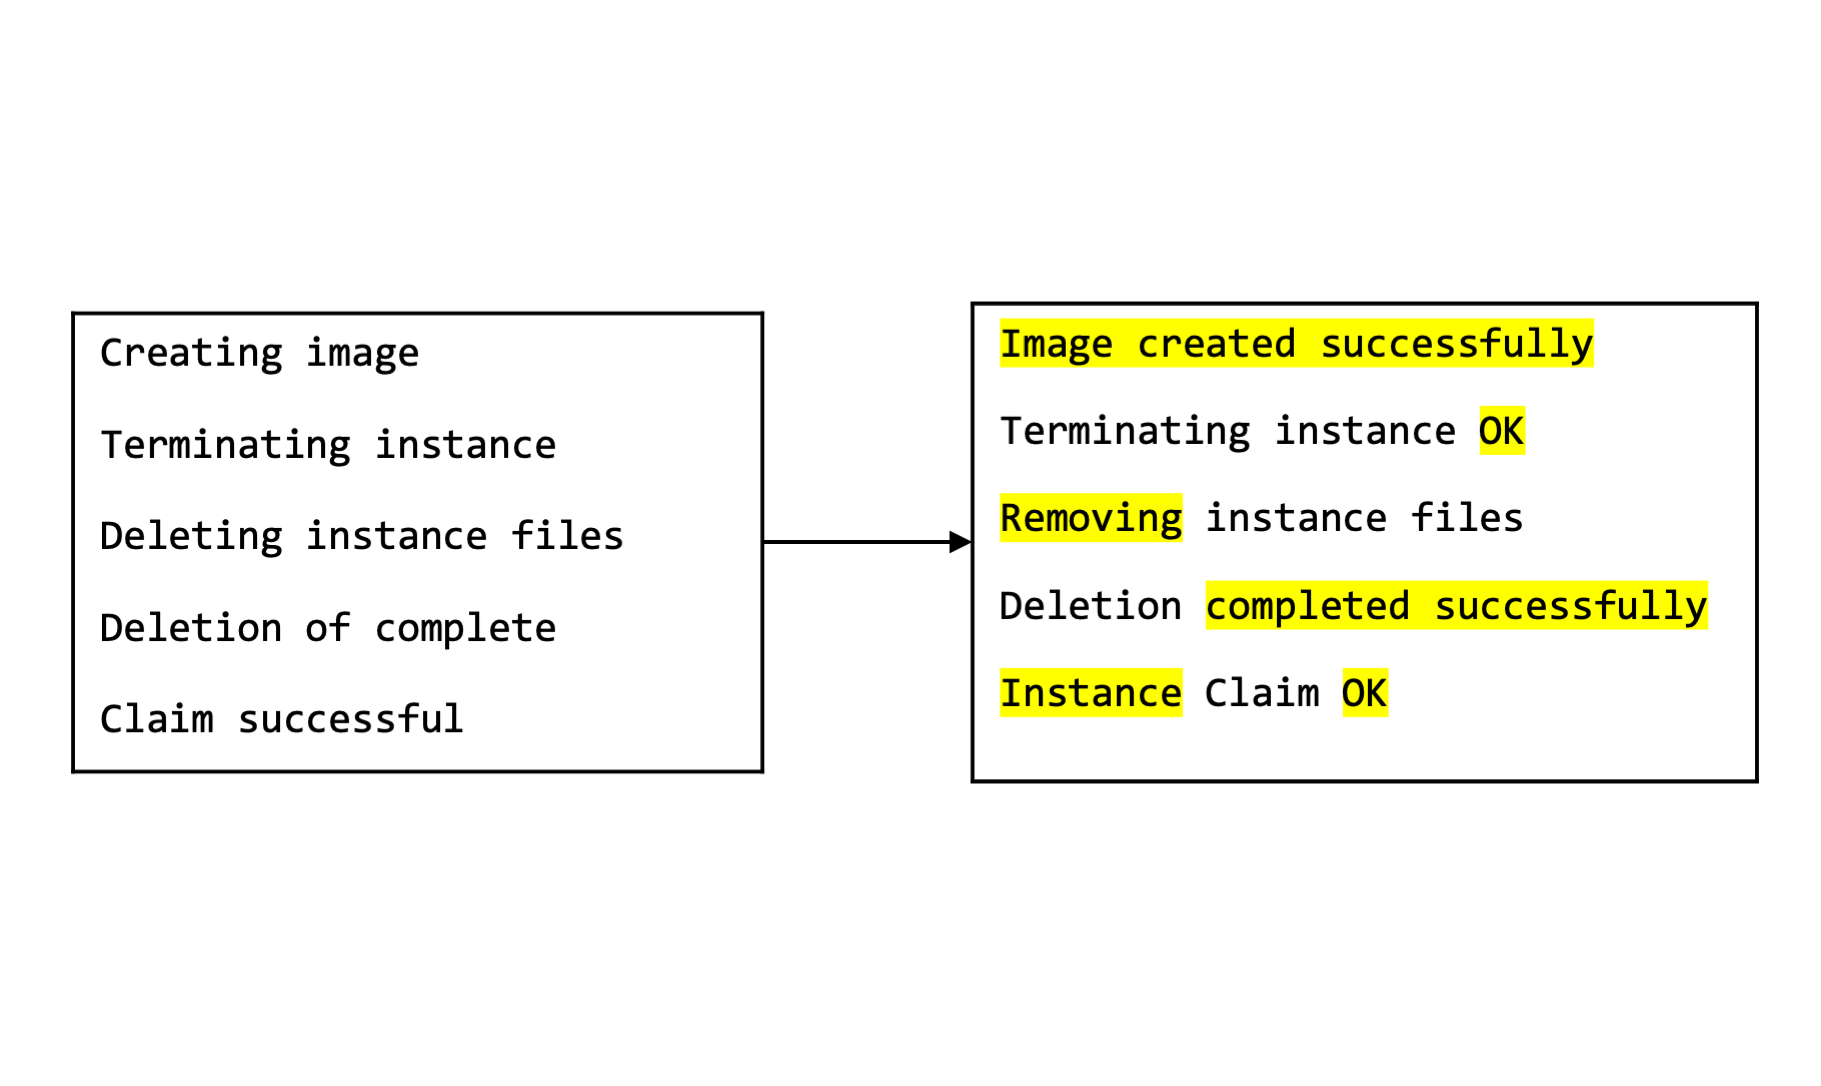
\includegraphics[width=10cm,height=6cm]{transfer_modifications.png}\\
  \caption{Changes on templates of the original dataset.}
  \label{fig:transfer_modifications}
\end{figure}




\section{Evaluation\label{sec:evaluation}}
In this section, the results of the evaluation between the two anomaly detection approaches, namely the regression-based approach and the classification-based approach are compared using three different language models, namely Bert, XL-Transformers and GPT-2. The pre-processing steps string cleansing and finetuning, as described \ref{sec:pre_processing} are investigated with regards to their potential on benefiting the quality of the word embeddings. Subsequently, the results of the evaluation using one dataset and the transfer learning approach are presented.

\subsection{String cleansing}
String cleansing, as described in \ref{sec:template_cleansing}, can potentially  improve distinguishability between templates drastically in the used dataset.
For Bert, the pairwise cosine distances before cleansing are depicted in figure \ref{fig:bert_before_cleansing}, after cleansing in figure \ref{fig:bert_after_cleansing}. The corresponding templates to the indices on the x and y axes before and after cleansing can be found in table \ref{tab:templates_before_cleansing} and table \ref{tab:templates_after_cleansing} respectively.
The cosine distances before and after cleansing for GPT-2 can be found in figure \ref{fig:gpt_before_cleansing} and figure \ref{fig:gpt_after_cleansing}, and for XL-Transformer in figure \ref{fig:xl_before_cleansing} and figure \ref{fig:xl_after_cleansing}, respectively. The average pairwise cosine distances between templates before and after cleansing can be seen in table \ref{tab:average_pairwise_cos_distances}.
Note that the cosine distances between templates appear to be relatively low for GPT-2 before and after cleansing. Even though cleansing results in a two-fold increase in the distances, the initial value is already very low. We can see how the distinguishability between templates increases for Bert and even more impressively for XL-Transformers. While Bert has a slightly higher average pairwise cosine distance before cleansing, XL-Transformers highly benefits from cleansing with an average value of 0.62. This underlines the importance of this step in order to meet the requirements postulated in \ref{sec:word_vectorization}, depending on the deployed language models.



\begin{table}[ht]
\centering
\begin{small}
\begin{tabular}{ p{1.3cm} p{2.5cm} p{2.5cm} }
\toprule
Model & Before cleansing & After cleansing\\
\midrule
XL & 0.2232 & 0.6223\\
Bert & 0.2416 & 0.4449\\
GPT-2 & 0.0024 & 0.0047 \\ 

\bottomrule
\end{tabular}
\caption{Average pairwise template cosine distances.}
\label{tab:average_pairwise_cos_distances}
\end{small}
\end{table}


\begin{figure}[!tbp]
  \centering
  \subfloat[Before cleansing.]{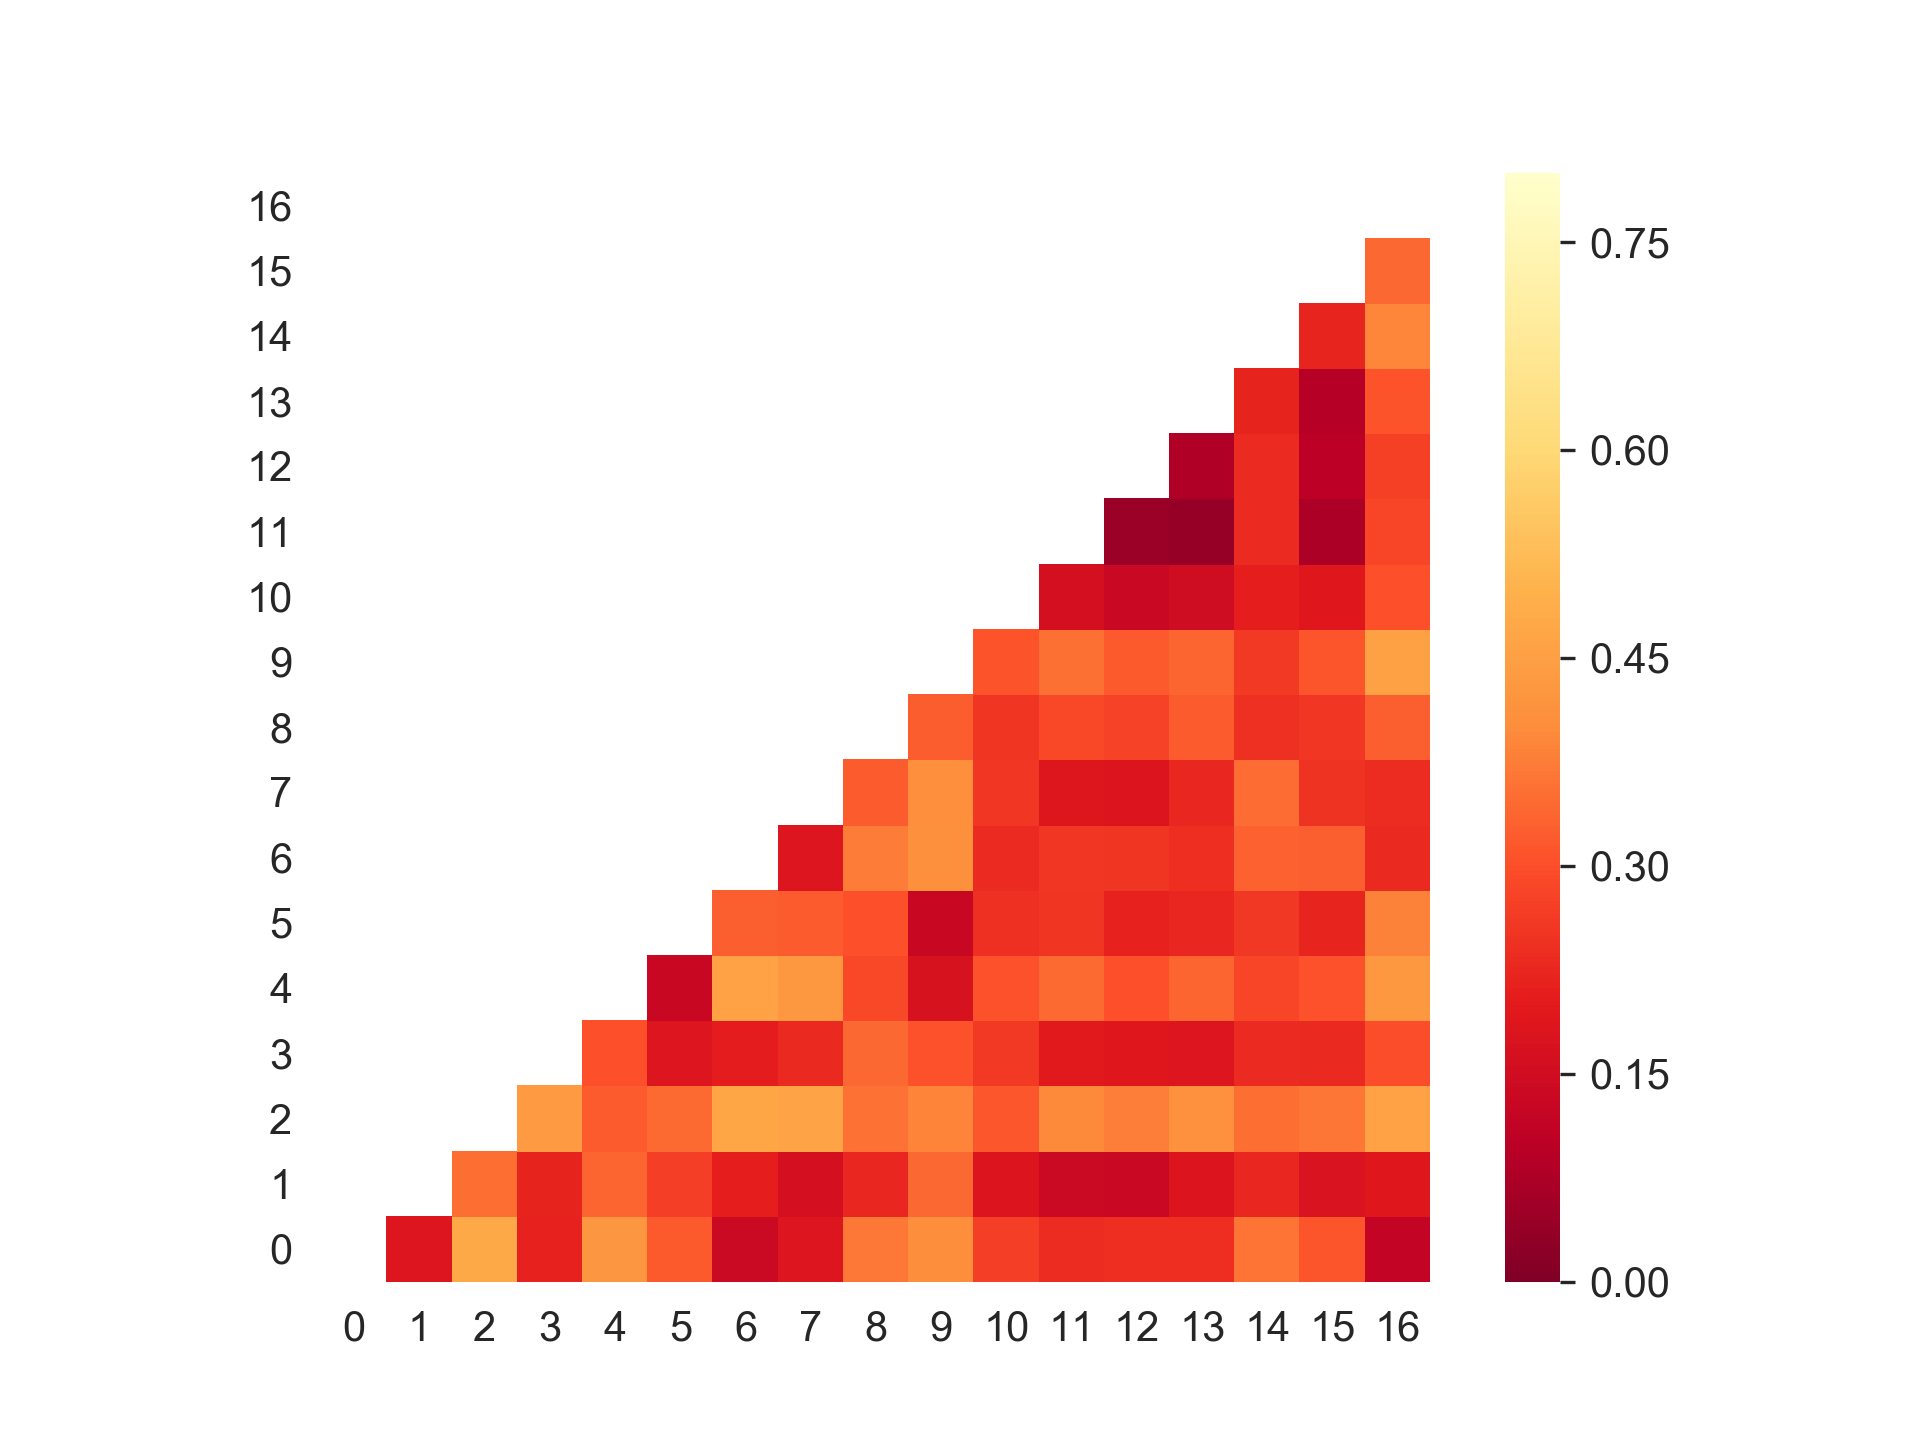
\includegraphics[width=0.5\textwidth]{bert_before_cleansing.png}\label{fig:bert_before_cleansing}}
  \hfill
  \subfloat[After cleansing.]{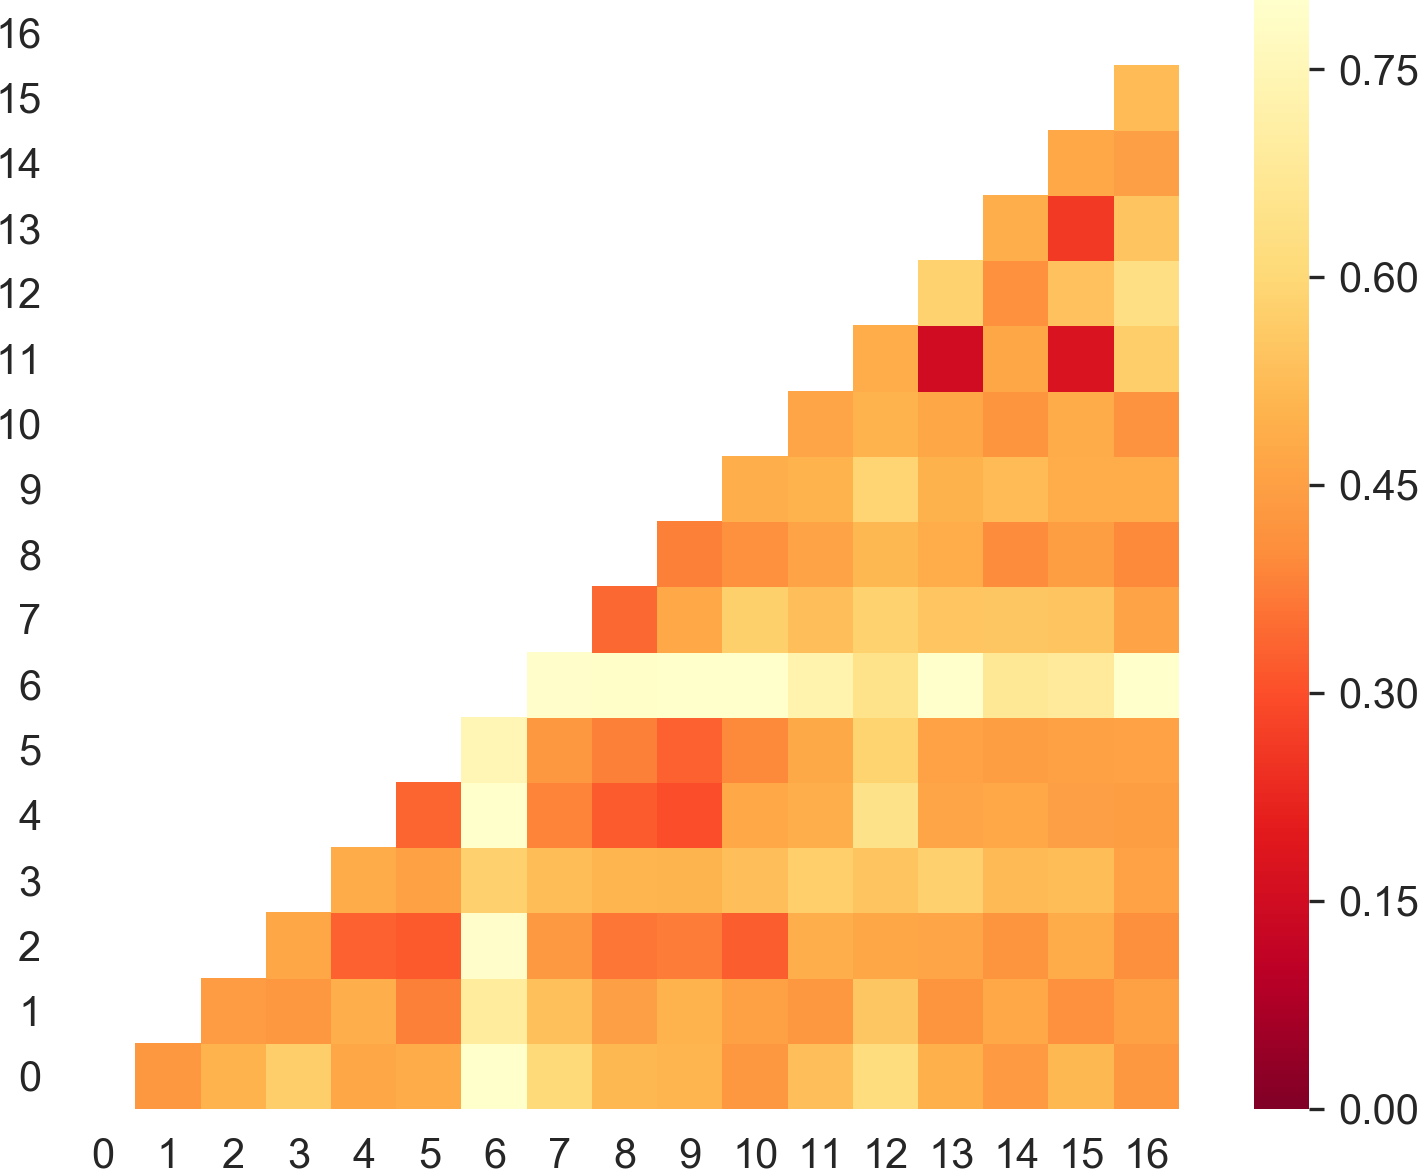
\includegraphics[width=0.5\textwidth]{bert_after_cleansing.png}\label{fig:bert_after_cleansing}}
  \caption{Bert pairwise template cosine distance.}
\end{figure}

\begin{figure}[!tbp]
  \centering
  \subfloat[Before cleansing.]{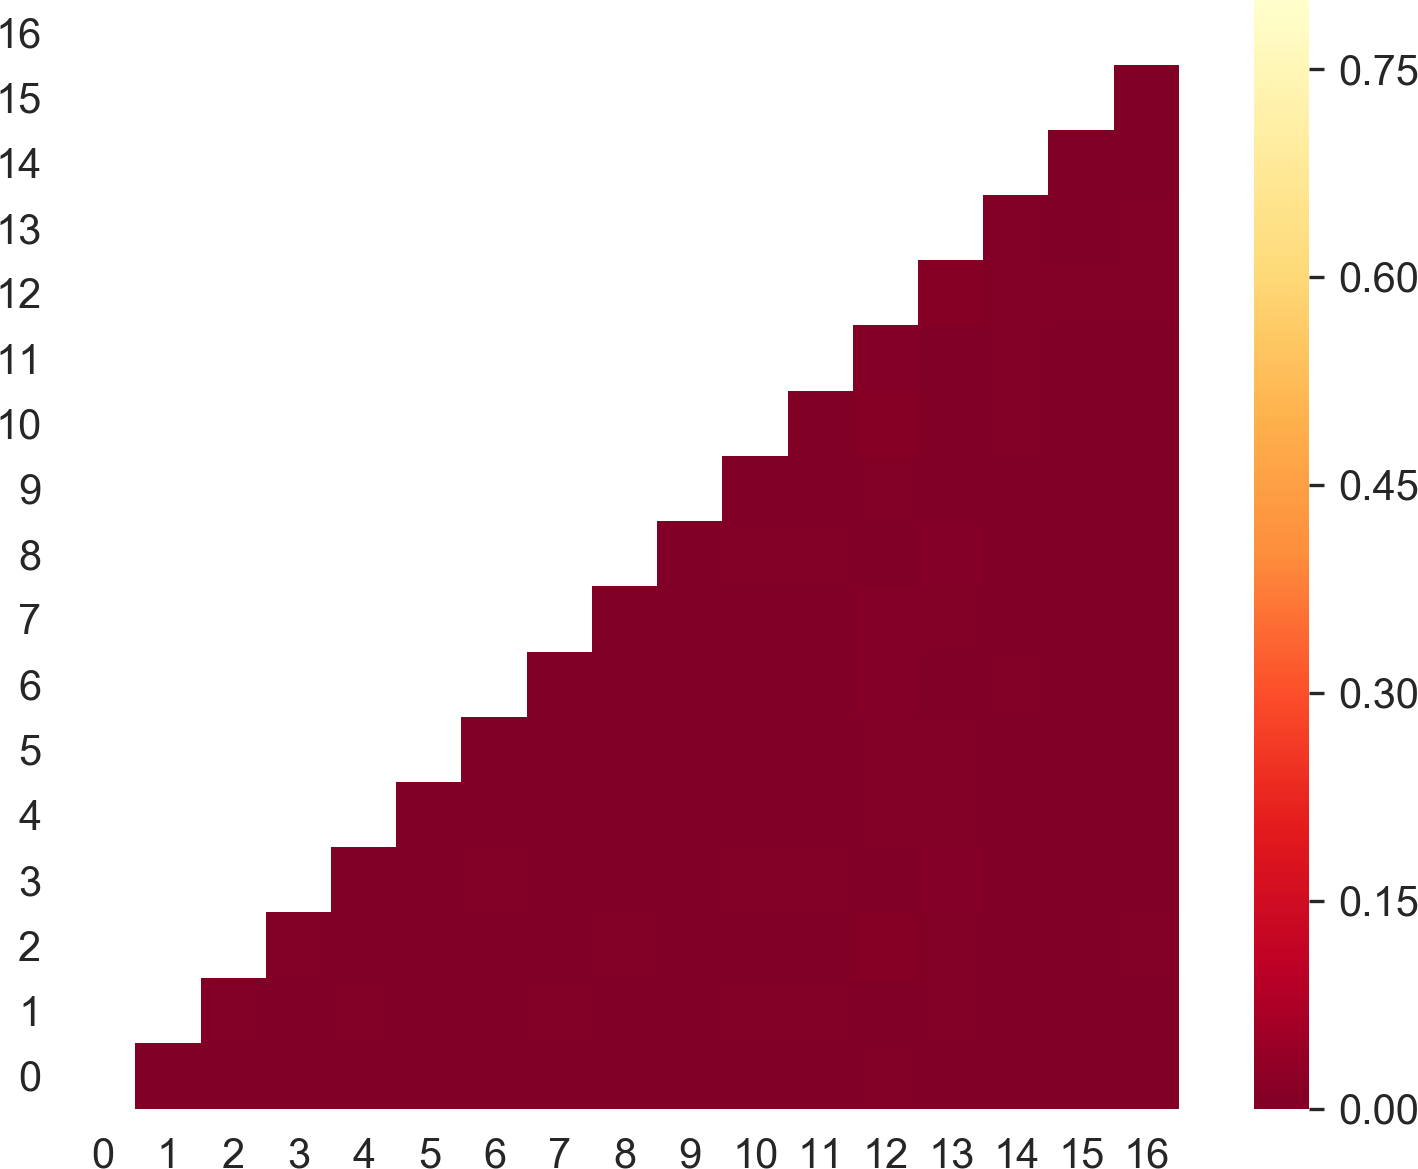
\includegraphics[width=0.5\textwidth]{gpt_before_cleansing.png}\label{fig:gpt_before_cleansing}}
  \hfill
  \subfloat[After cleansing.]{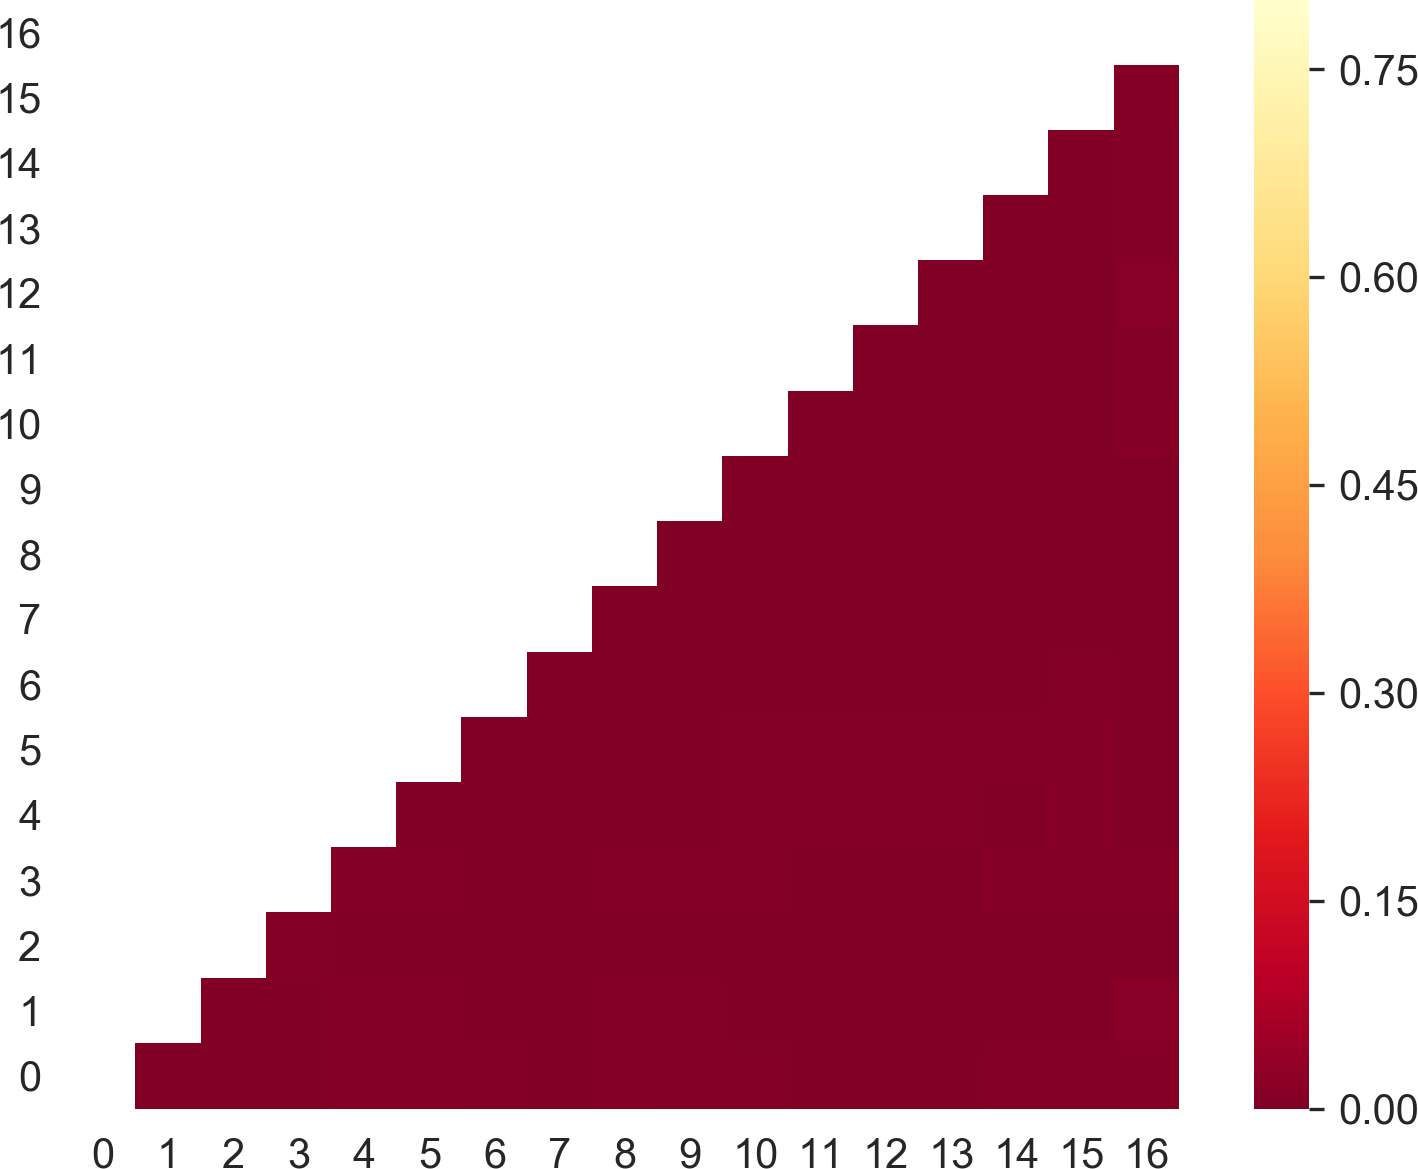
\includegraphics[width=0.5\textwidth]{gpt_after_cleansing.png}\label{fig:gpt_after_cleansing}}
  \caption{GPT-2 pairwise template cosine distance.}
\end{figure}

\begin{figure}[!tbp]
  \centering
  \subfloat[Before cleansing.]{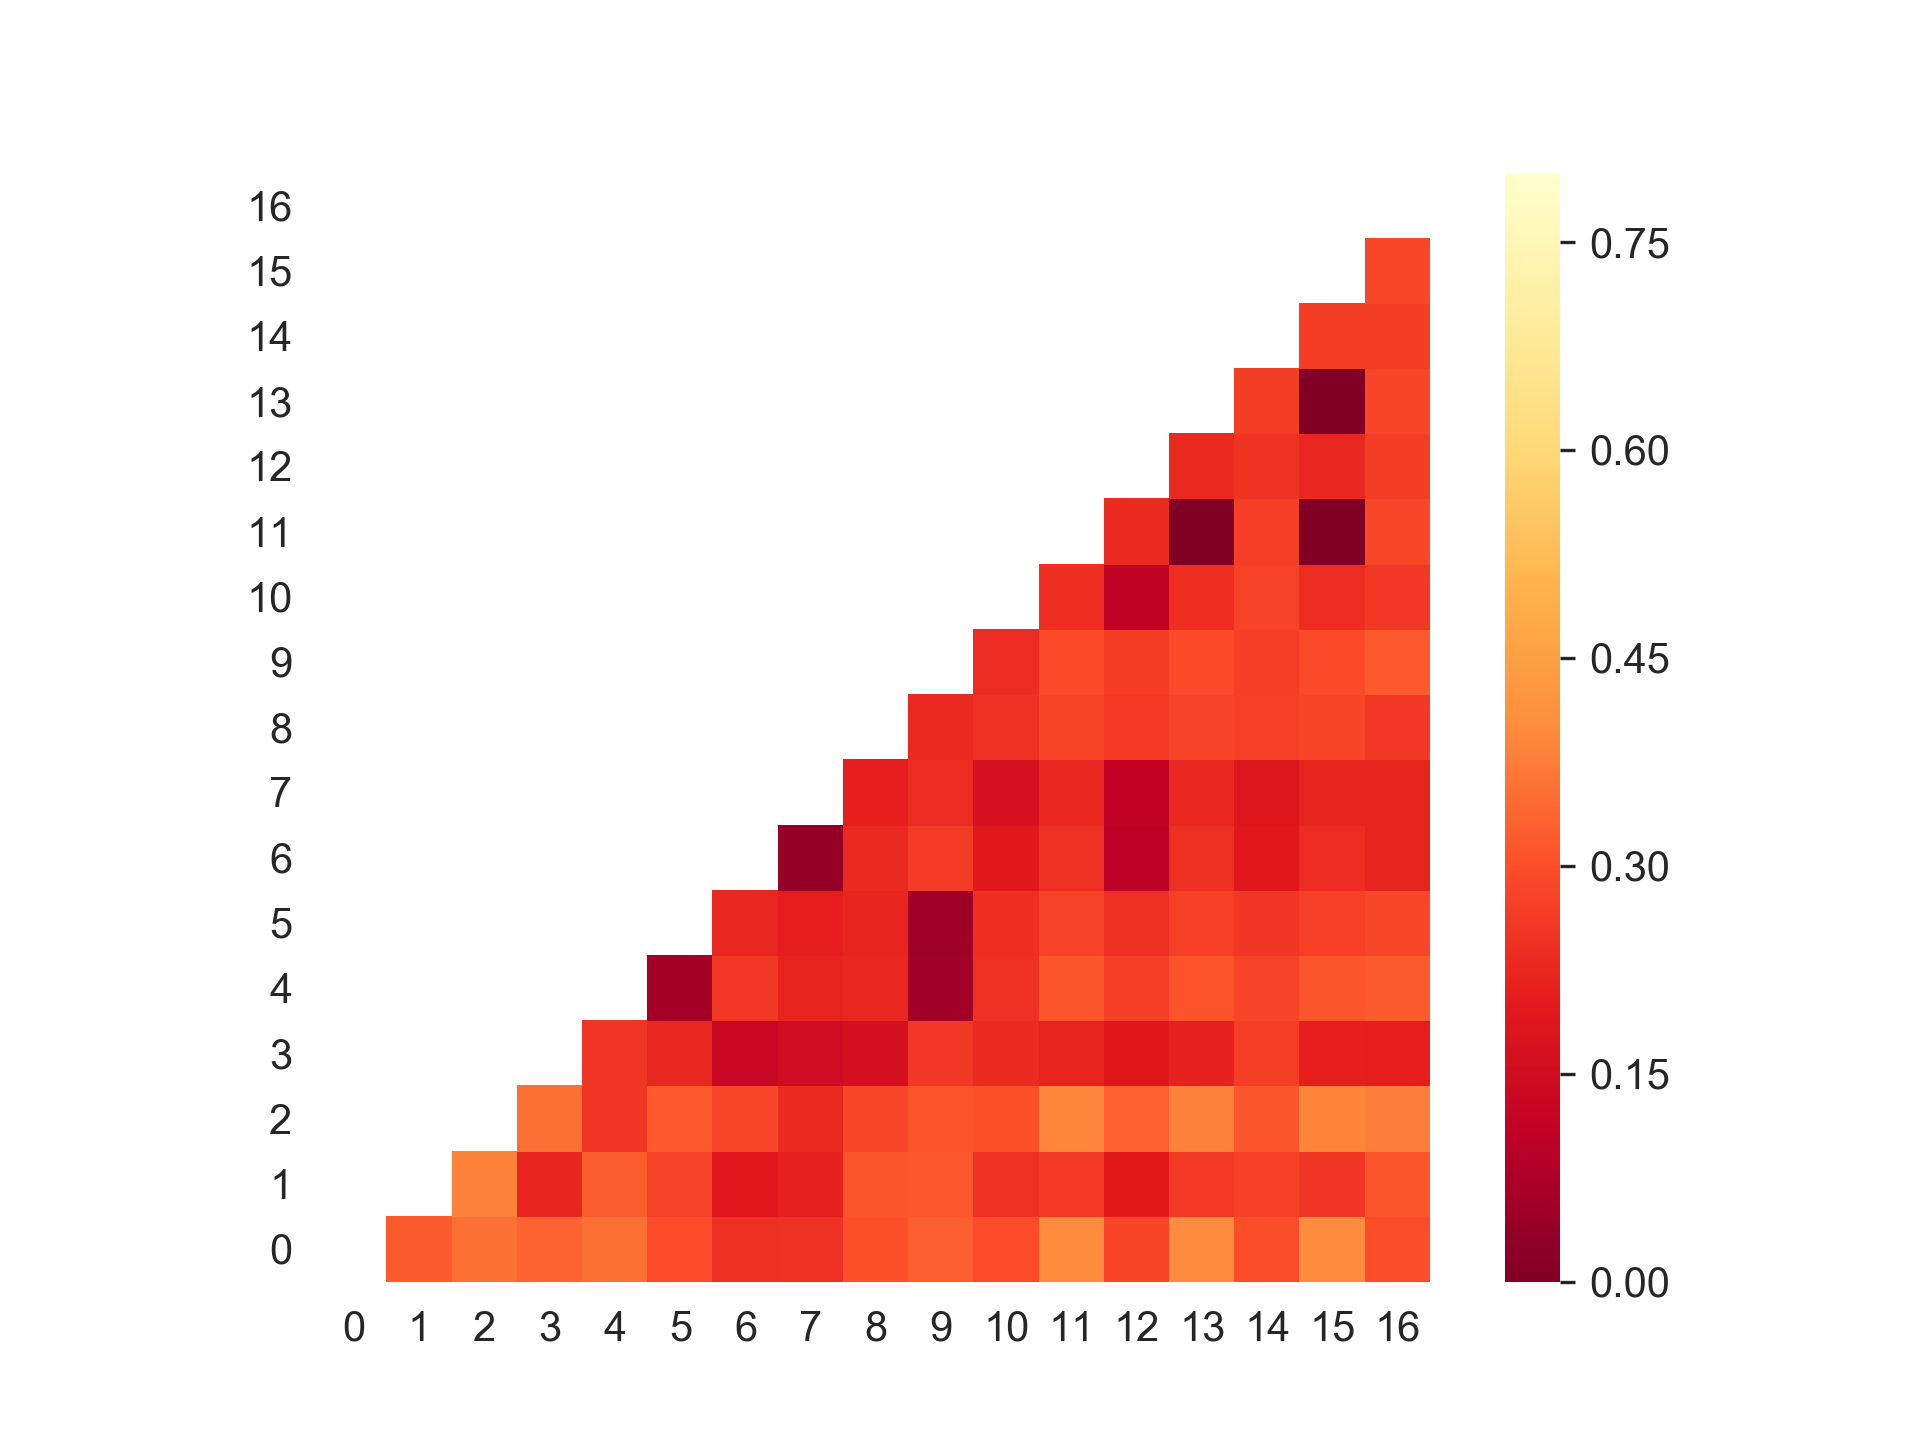
\includegraphics[width=0.5\textwidth]{xl_before_cleansing.png}\label{fig:xl_before_cleansing}}
  \hfill
  \subfloat[After cleansing.]{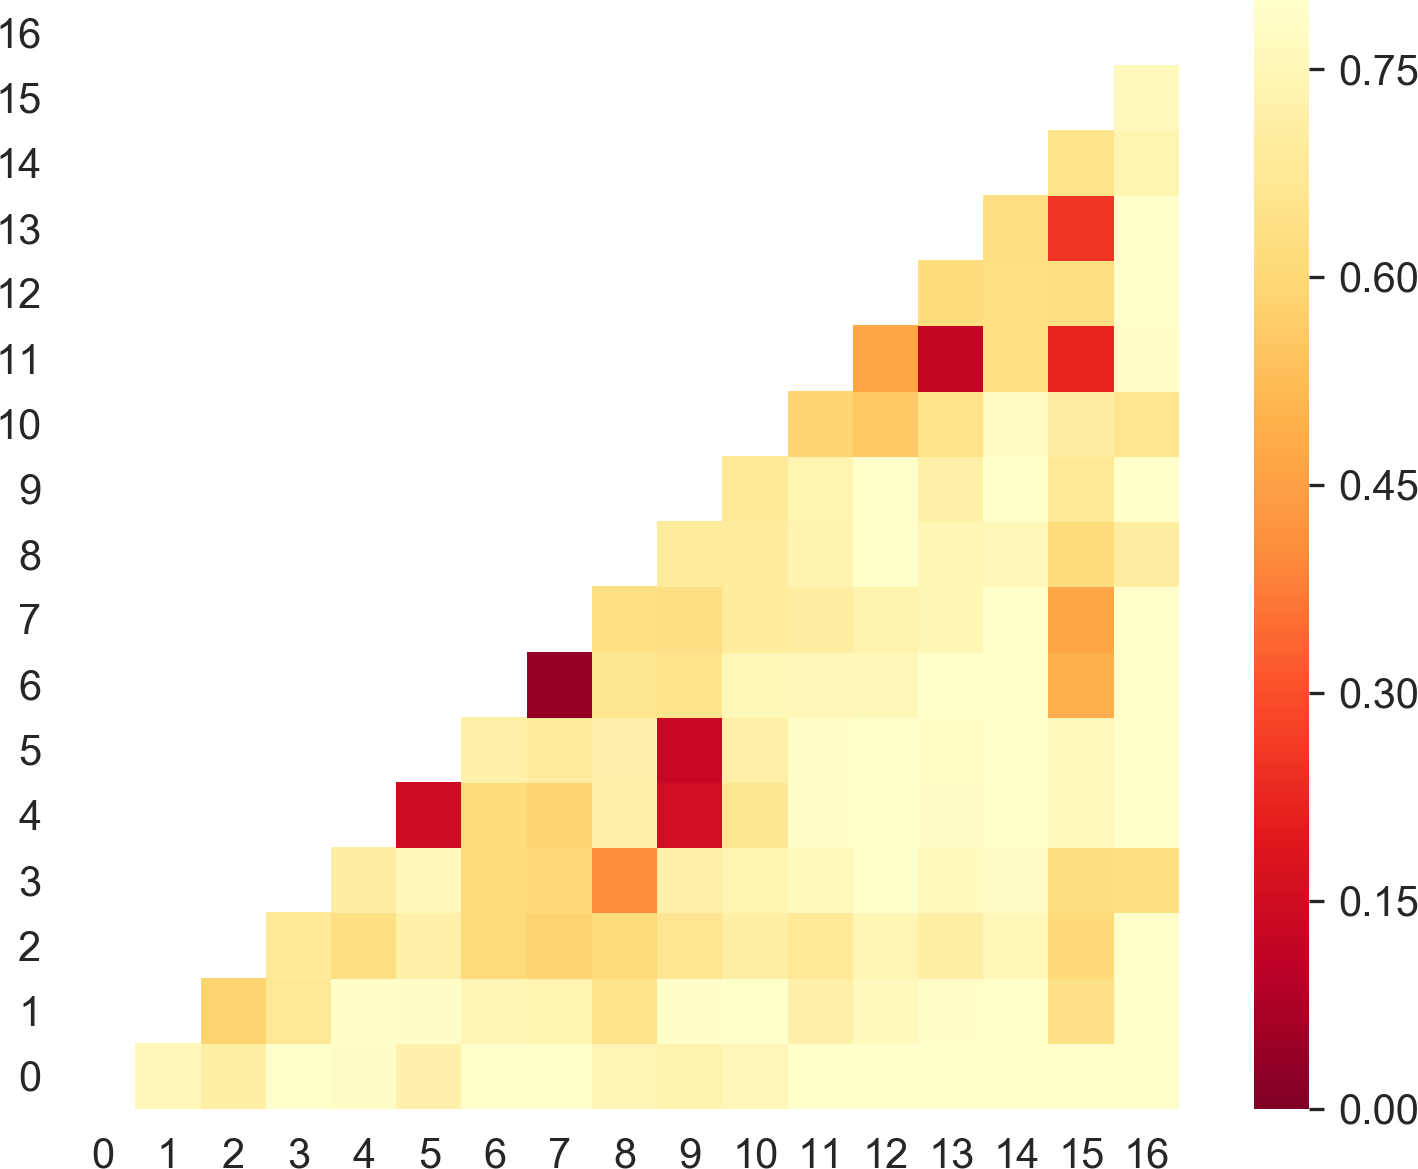
\includegraphics[width=0.5\textwidth]{xl_after_cleansing.png}\label{fig:xl_after_cleansing}}
  \caption{XL-Transformers pairwise template cosine distance.}
\end{figure}




\begin{table}[ht]
\begin{small}
\centering
\begin{tabular}{ c l } 
\toprule
Index & Template \\
\midrule
0 & $\langle*\rangle$ Creating image\\
1 & $\langle*\rangle$ VM $\langle*\rangle$ (Lifecycle Event)\\
2 & $\langle*\rangle$ During sync\_power\_state the instance has a pending task (spawning). Skip.\\
3 & $\langle*\rangle$ Instance $\langle*\rangle$ successfully.\\
4 & $\langle*\rangle$ Took $\langle*\rangle$.$\langle*\rangle$ seconds to $\langle*\rangle$ the instance on the hypervisor.\\
5 & $\langle*\rangle$ Took $\langle*\rangle$.$\langle*\rangle$ seconds to build instance.\\
6 & $\langle*\rangle$ Terminating instance\\
7 & $\langle*\rangle$ Deleting instance files $\langle*\rangle$\\
8 & $\langle*\rangle$ Deletion of $\langle*\rangle$ complete\\
9 & $\langle*\rangle$ Took $\langle*\rangle$.$\langle*\rangle$ seconds to deallocate network for instance.\\
10 & $\langle*\rangle$ Attempting claim: memory $\langle*\rangle$ MB, disk $\langle*\rangle$ GB, vcpus $\langle*\rangle$ CPU\\
11 & $\langle*\rangle$ Total memory: $\langle*\rangle$ MB, used: $\langle*\rangle$.$\langle*\rangle$ MB\\
12 & $\langle*\rangle$ memory limit: $\langle*\rangle$.$\langle*\rangle$ MB, free: $\langle*\rangle$.$\langle*\rangle$ MB\\
13 & $\langle*\rangle$ Total disk: $\langle*\rangle$ GB, used: $\langle*\rangle$.$\langle*\rangle$ GB\\
14 & $\langle*\rangle$ $\langle*\rangle$ limit not specified, defaulting to unlimited\\
15 & $\langle*\rangle$ Total vcpu: $\langle*\rangle$ VCPU, used: $\langle*\rangle$.$\langle*\rangle$ VCPU\\
16 & $\langle*\rangle$ Claim successful\\
\bottomrule
\end{tabular}
\caption{Templates before cleansing}
\label{tab:templates_before_cleansing}
\end{small}
\end{table}



\begin{table}[ht]
\begin{small}
\centering
\begin{tabular}{ c l } 
\toprule
Index & Template \\
\midrule
0 & Creating image\\
1 & VM  Lifecycle Event\\
2 & During sync power state the instance has a pending task spawning Skip\\
3 & Instance  successfully\\
4 & Took  seconds to  the instance on the hypervisor\\
5 & Took  seconds to build instance\\
6 & Terminating instance\\
7 & Deleting instance files\\
8 & Deletion of complete\\
9 & Took  seconds to deallocate network for instance\\
10 & Attempting claim memory  MB disk  GB vcpus  CPU\\
11 & Total memory  MB used  MB\\
12 & memory limit  MB free  MB\\
13 & Total disk  GB used  GB\\
14 & limit not specified defaulting to unlimited\\
15 & Total vcpu  VCPU used  VCPU\\
16 & Claim successful\\
\bottomrule
\end{tabular}
\caption{Templates after cleansing}
\label{tab:templates_after_cleansing}
\end{small}
\end{table}

\subsection{Finetuning}
As described in \ref{sec:finetuning}, finetuning can potentially help to produce word embeddings that are more adequate for solving a certain task, it is thus desirable to produce word embeddings that help solving the task of anomaly detection better. As described in \ref{sec:word_vectorization}, a high cosine distance between semantically different templates is required. The dataset that consists of the templates in table \ref{tab:templates_after_cleansing} has been chosen for finetuning. Since the pre-trained language models at hand (namely \textit{bert-base-uncased} and \textit{gpt2}) have been trained on a large corpus, finetuning would also need to be executed on a sufficiently large corpus. Since this is not the case, the results of finetuning for a maximum of four epochs, as suggested by the Bert authors \cite{devlin2018bert}, does not yield the desired results. As it can be seen in figure \ref{fig:cos_distance_finetuning}, it was not possible to increase the cosine distances between templates on the task of Masked LM (as described in \ref{Bert}), compared to the cosine distances depicted in figure \ref{fig:bert_after_cleansing}. The average distance between templates dropped to 0.3016 from 0.4449. The fact that the loss on the evaluation part of the dataset is not decreasing adequately, as shown in figure \ref{fig:finetuning_loss}, shows that training on such a small corpus is not able to generalise well enough, which makes finetuning on the default learning task not useful in this case. Since the Huggingface Transformers library does not offer out of the box finetuning interfaces for GPT-2 and XL-Transformers on the same task as for Bert, they are not further investigated for finetuning.

\begin{figure}[H]
  \centering
  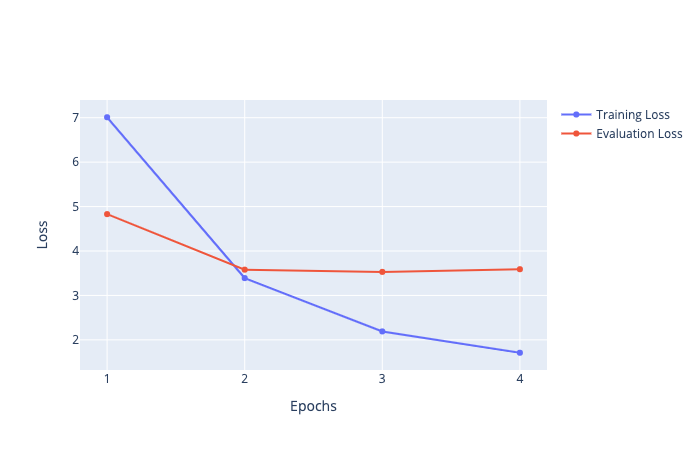
\includegraphics[width=12cm,height=8.5cm]{finetuning_loss.png}\\
  \caption{Training and evaluation loss for finetuning on masked LM.}
  \label{fig:finetuning_loss}
\end{figure}

\begin{figure}[h]
  \centering
  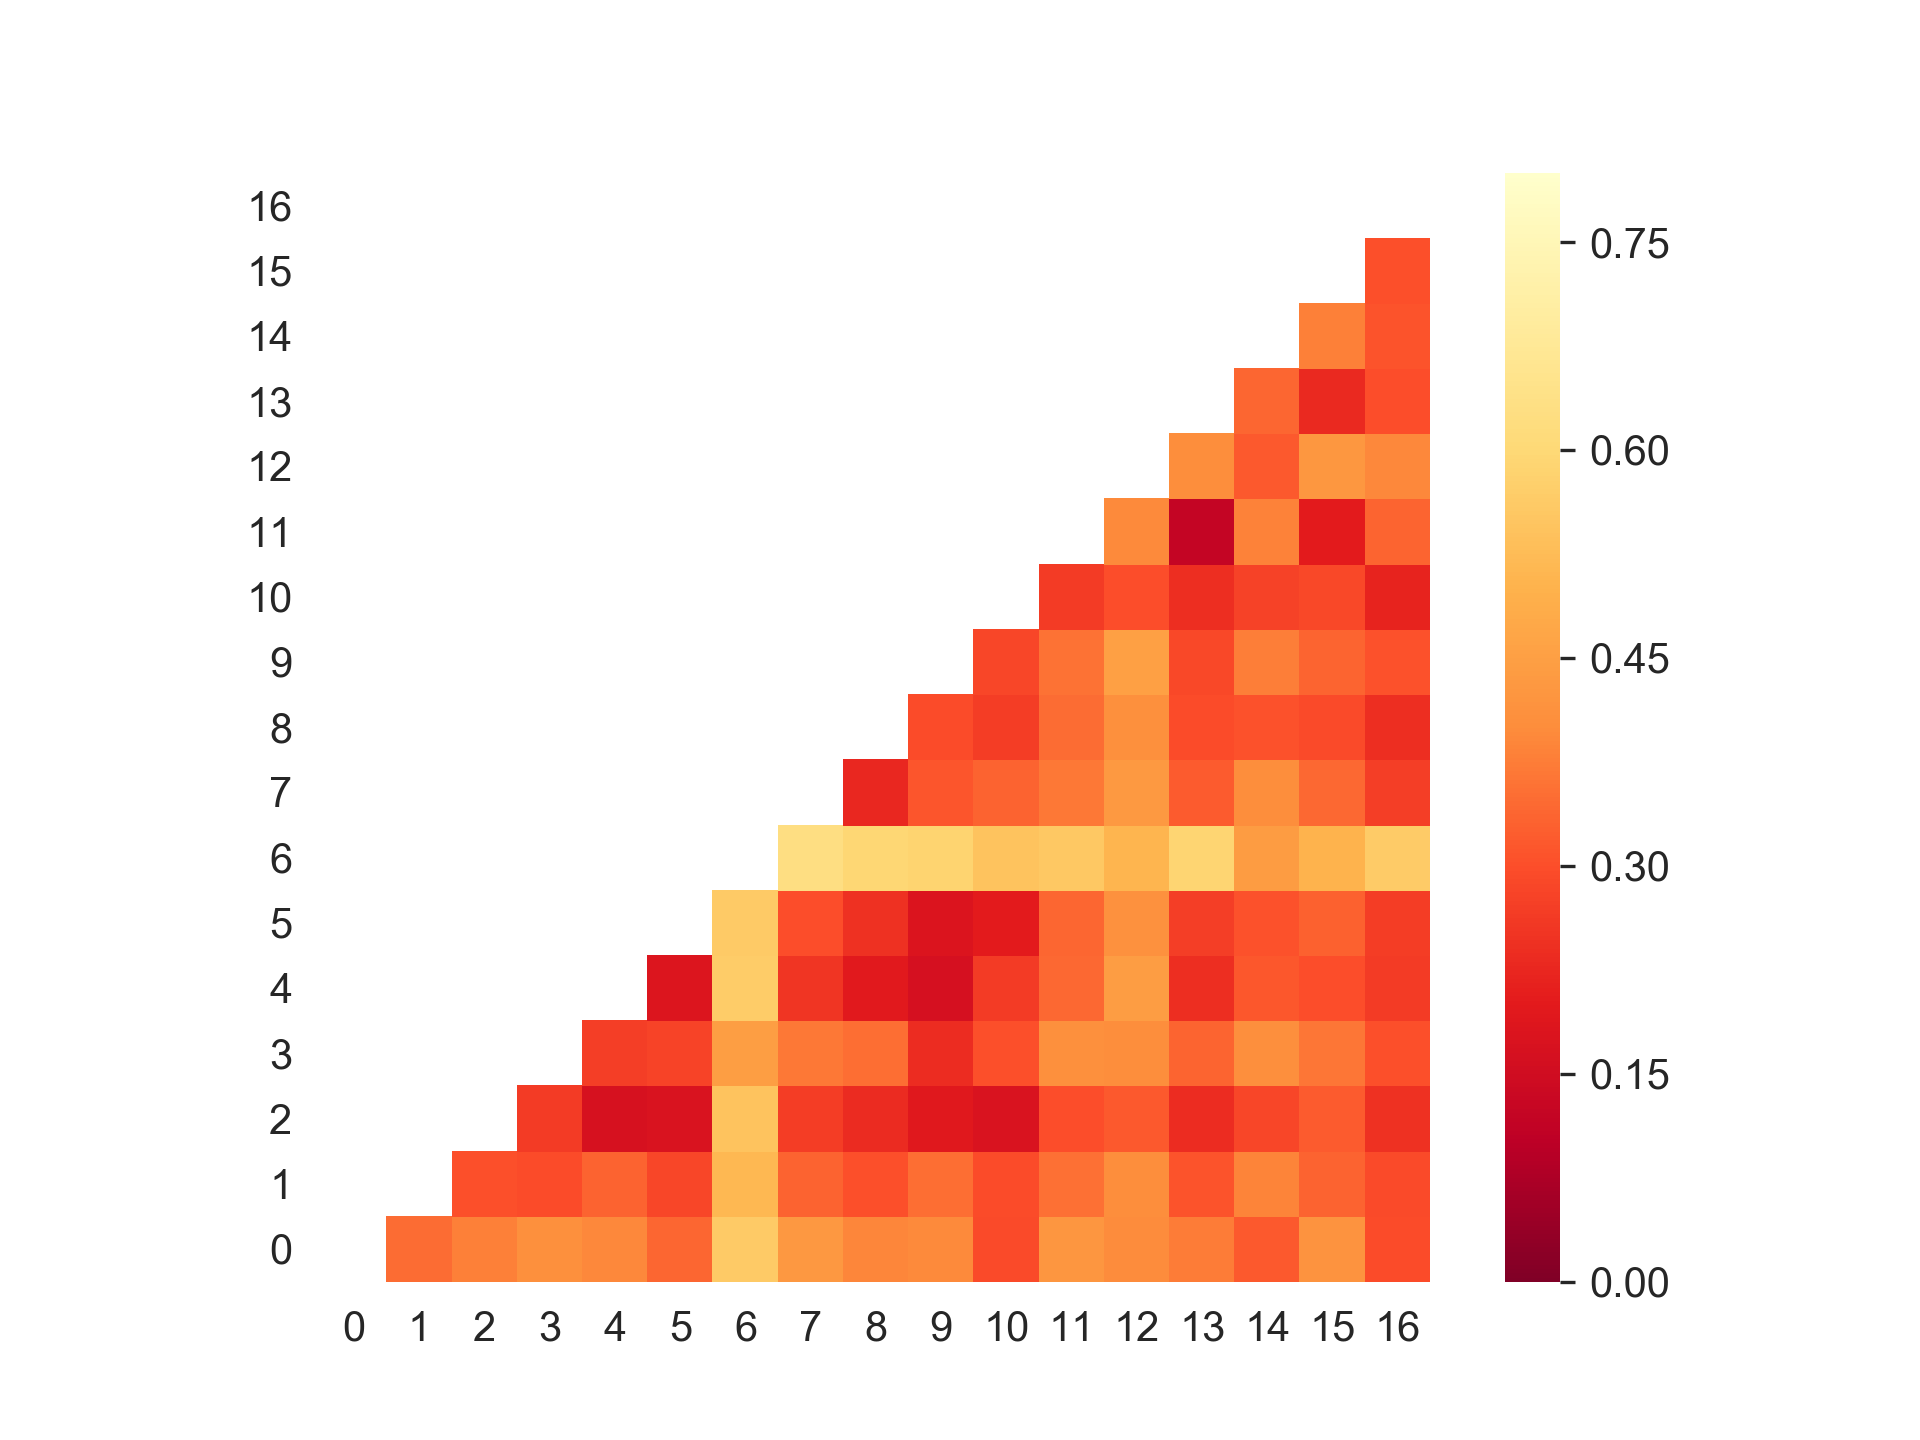
\includegraphics[width=12cm,height=9cm]{bert_finetuning_cleansed.png}\\
  \caption{Cosine distance between templates after cleansing and finetuning}
  \label{fig:cos_distance_finetuning}
\end{figure}


\subsection{Hyperparameters}
In order to find well-suited parameters for the LSTM model, it was first applied to the problem using a minimal configuration. With the help of a grid-search, running simulations with different configurations, the following hyperparameters have proven to yield the most satisfying results:
\begin{itemize}
	\item 512 hidden units for the bidirectional LSTM, with one layer
	\item two fully connected layers with 512 units $\rightarrow$ 256 units $\rightarrow$ output size
	\item dropout of 0.1 between every layer
	\item input sequence length of 7
	\item 60 Epochs of training
\end{itemize}

%%%%%%%%%%%%
% REGRESSION 
%%%%%%%%%%%%
\subsection{Regression-based approach using one dataset\label{sec:results-regression}}
In this subsection, the results of the regression-based approach, with various alterations using the different language models, are presented. In order to evaluate the robustness of the language models to the evolution of log events, alterations as described in \ref{sec:logs_alteration} are injected at different ratios. The impact on detecting injected anomalies after alterations on the sequence of logs are injected, i.e. deleting, shuffling and duplicating events are summarised in figure \ref{fig:results_regression_sequential}. Alterations are not injected all at the same time, but independently from each other, the results in the figures are average values of all experiments with alterations on the log sequences. Results broken down by each alteration can be found in the appendix \ref{appendix:regression}. It is evident, that GPT-2 performs better than Bert and XL-Transformers on both the F1-score and precision.

In contrast to the alterations on the log sequences, alterations on the log events themselves, i.e. inserting, removing and replacing words are also of interest. The results of this experiment can be seen in figure \ref{fig:results_regression_words}. Again, the alterations are not injected all at once, but independently - the figure shows averaged results.

Another aspect that is evaluated, is the impact of the input sequence length, i.e. the number of concatenated log events for which the next log event shall be predicted, on the ability of the model to detect anomalies. The results of this evaluation can be seen in \ref{fig:seq_len_regression}. Bert and GPT-2 seem to profit slightly from sequence lengths longer than 6 or 7, whereas the quality of results for XL-Transformers are not as affected from the input sequence length, but are generally lower.

\begin{comment}
\begin{figure}[h]
  \centering
  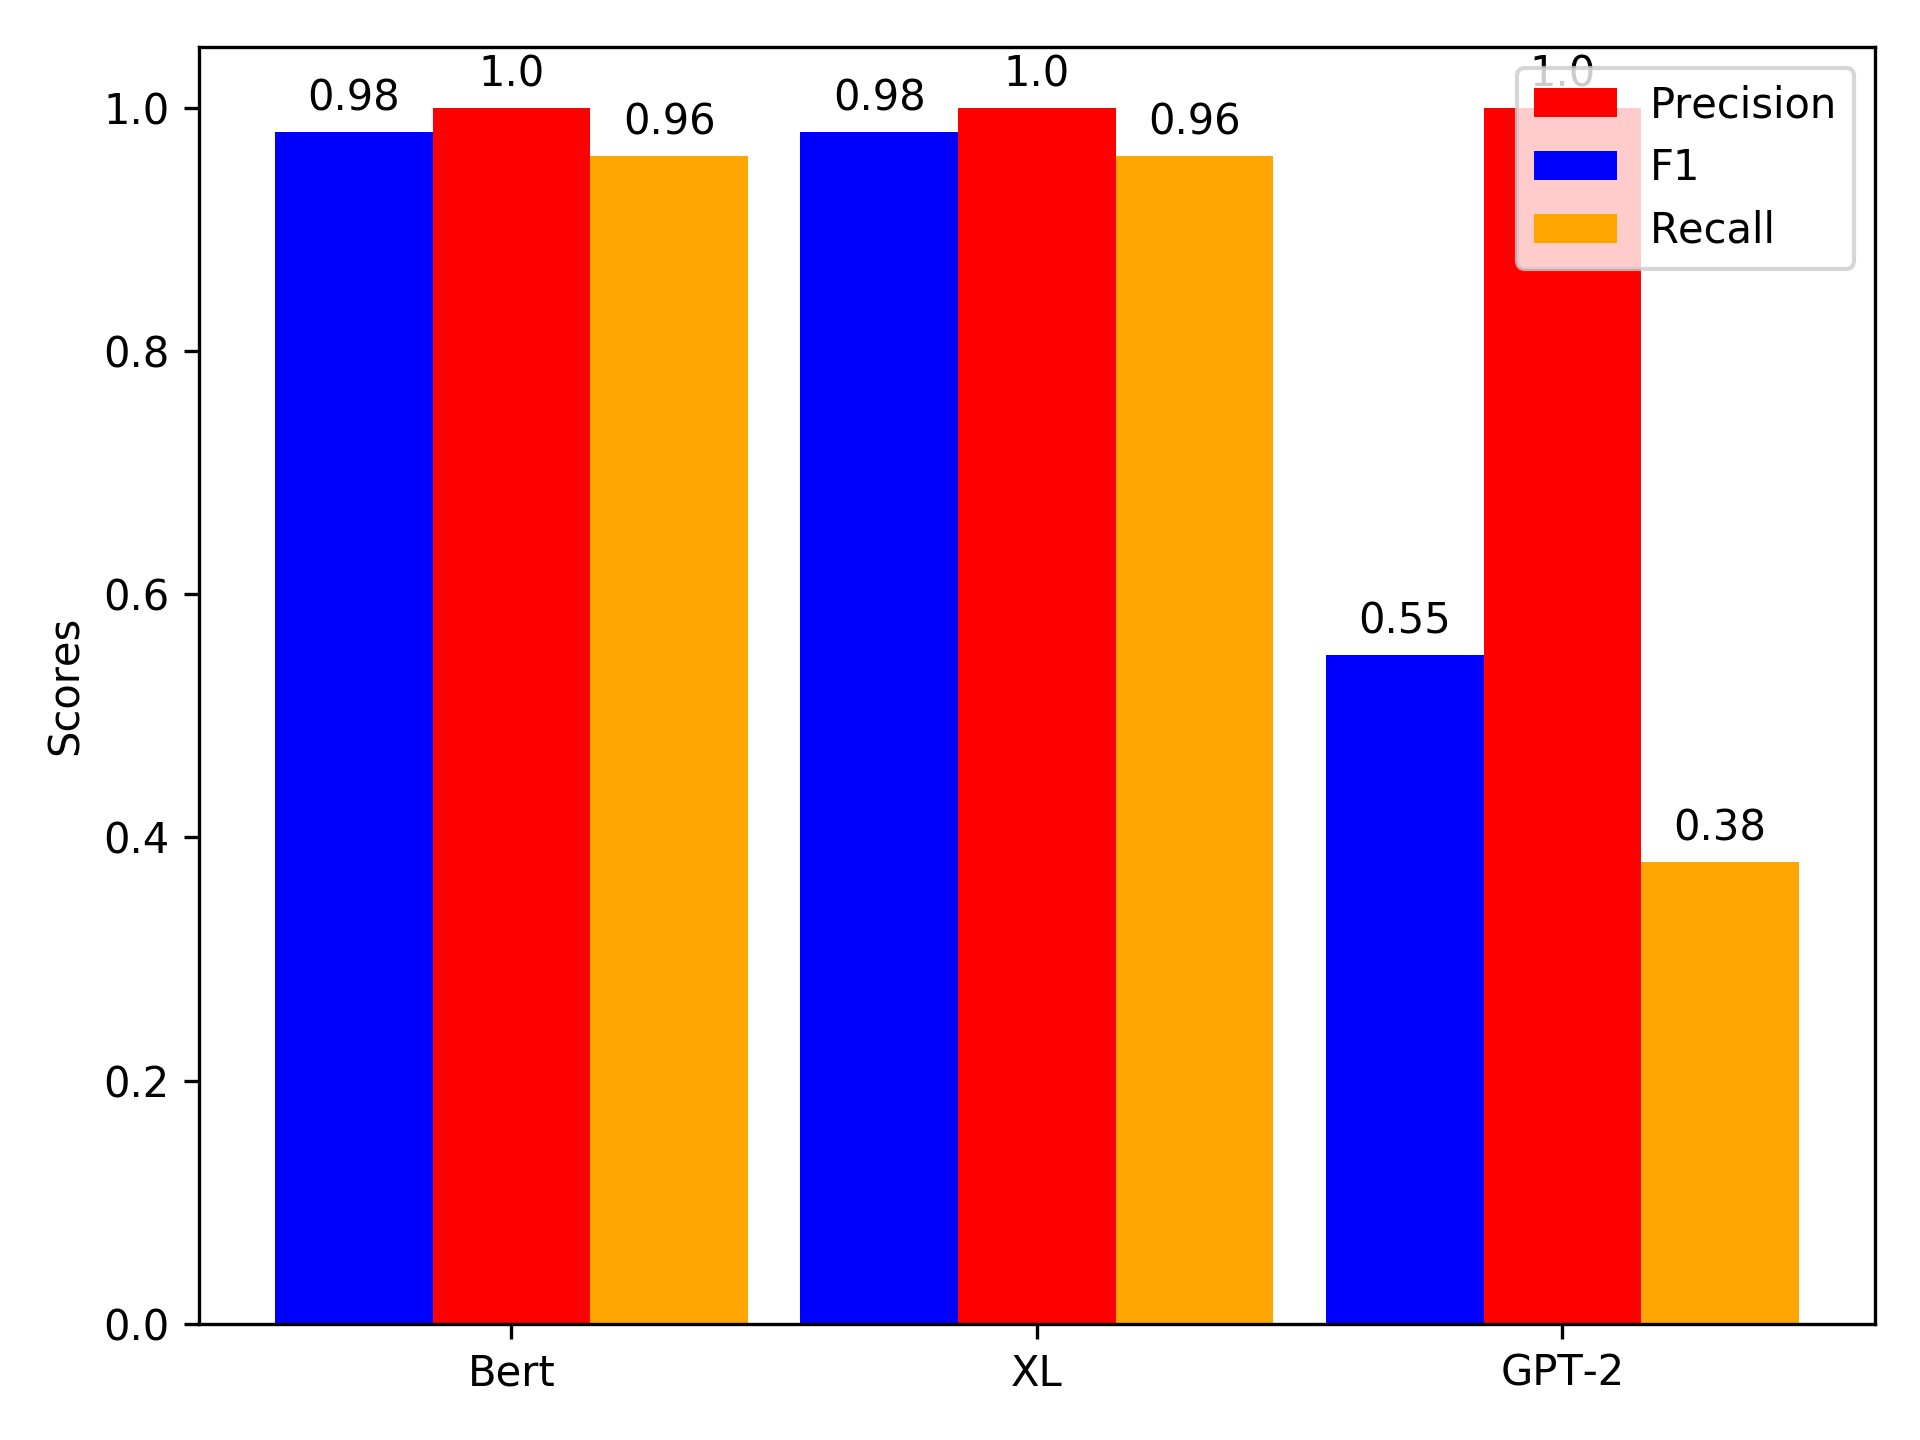
\includegraphics[width=6cm,height=4.5cm]{results/regression_sequence/regression_reverse.png}\\
  \caption{Scores for detecting reversed order of log events, using regression.}
  \label{fig:regression_reverse_order}
\end{figure}
\end{comment}

\begin{figure*}[ht!]
  \centering
  \captionsetup{justification=centering}
   \subfloat[5\% alteration\label{fig:results_regression_sequential_5}]{%
      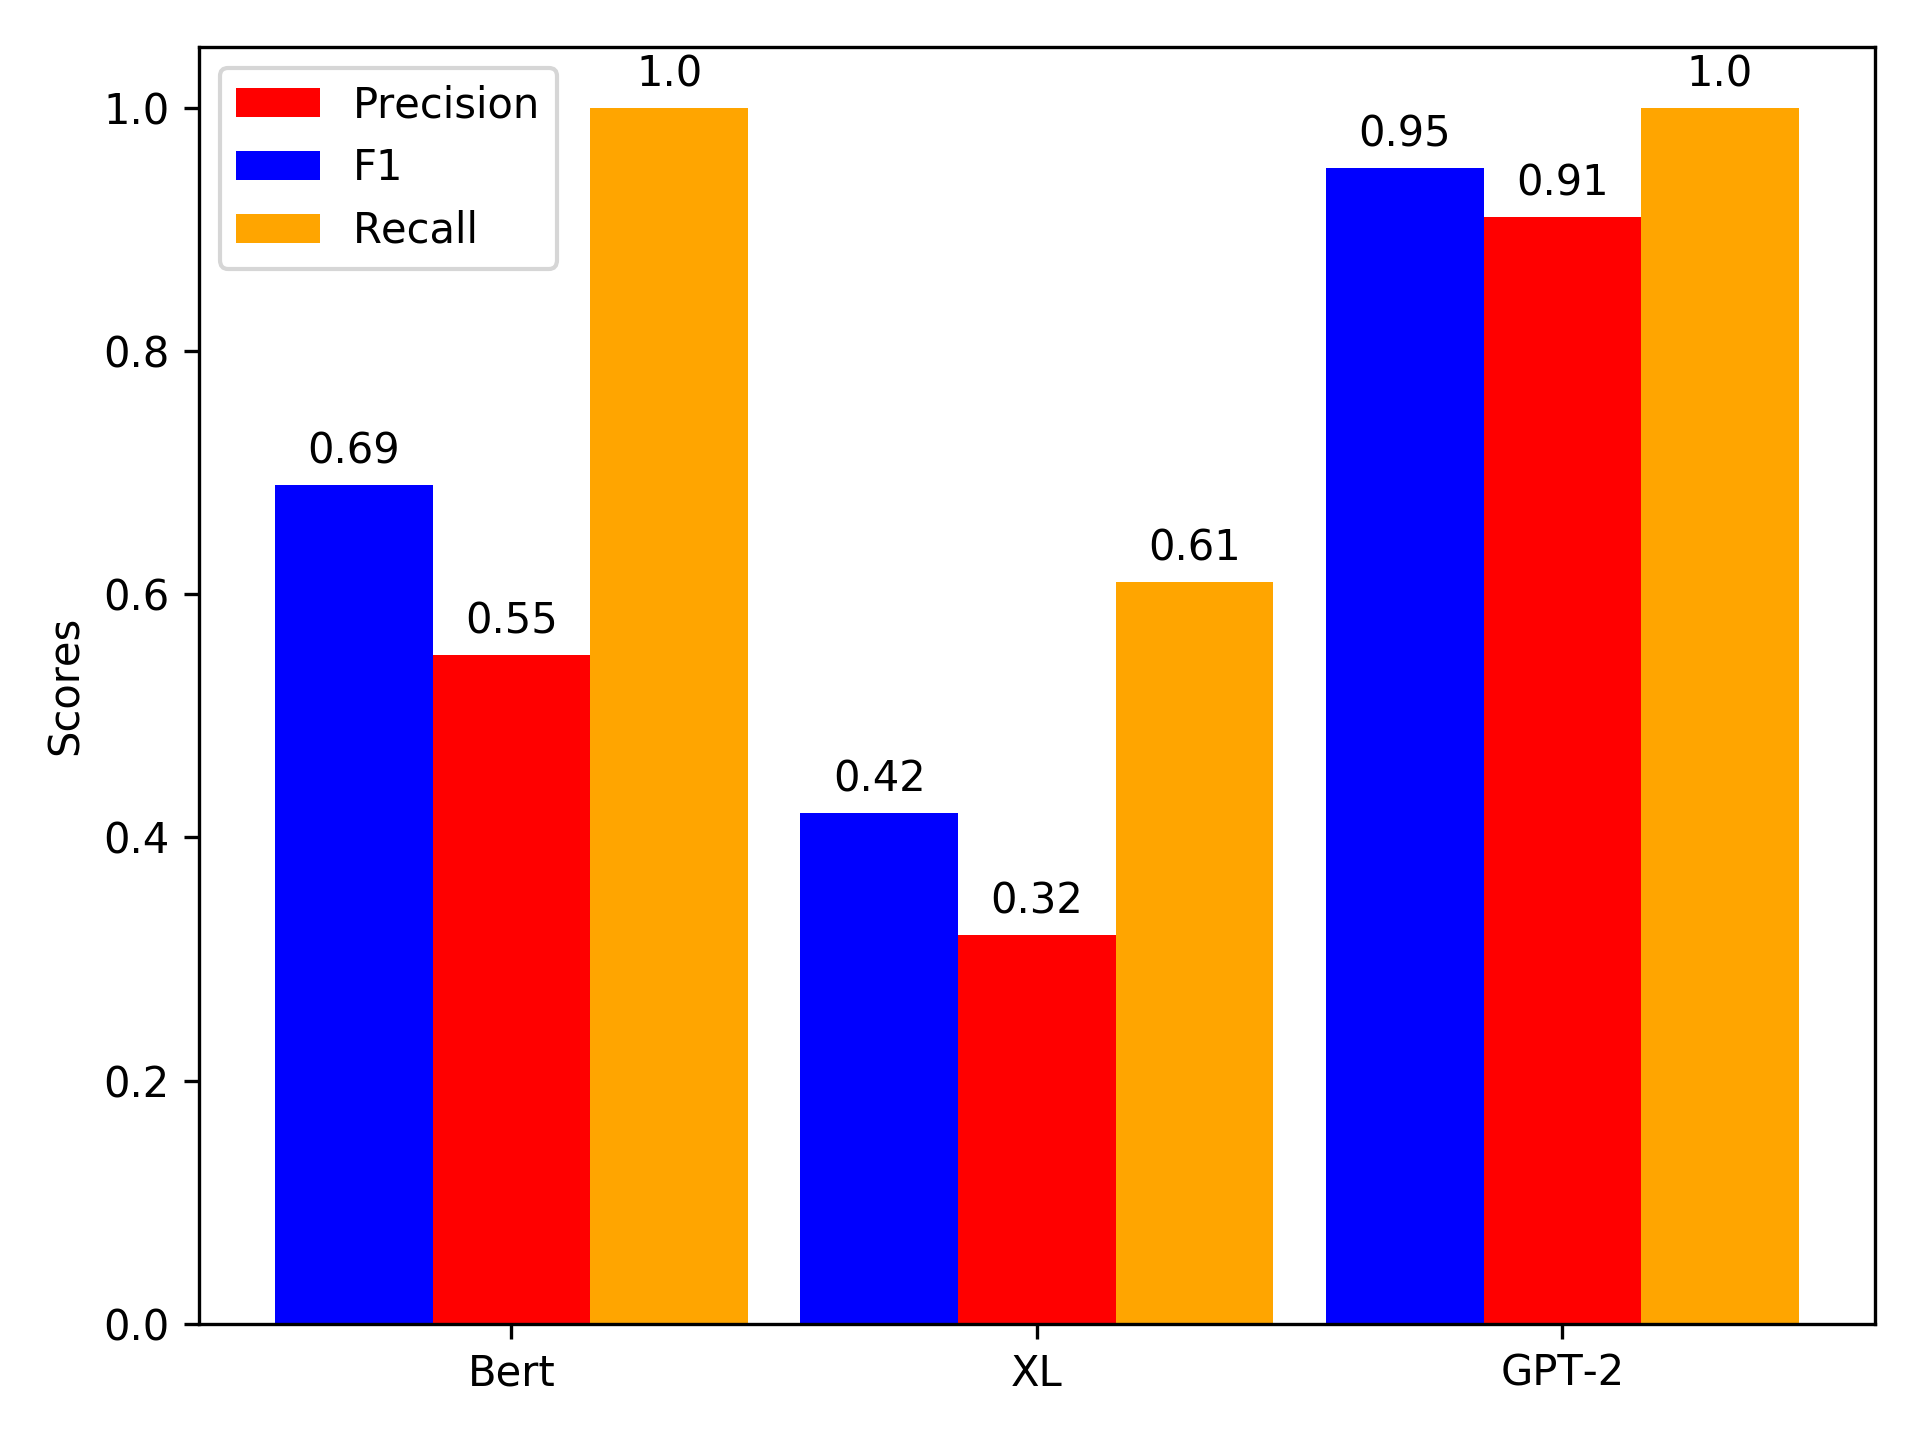
\includegraphics[trim={1cm 0.5cm 0cm 1cm}, width=0.322\textwidth]{results/average/regression_sequential_average_ratio_0.05.png}}
\hspace{\fill}
   \subfloat[10\% alteration\label{fig:results_regression_sequential_10} ]{%
      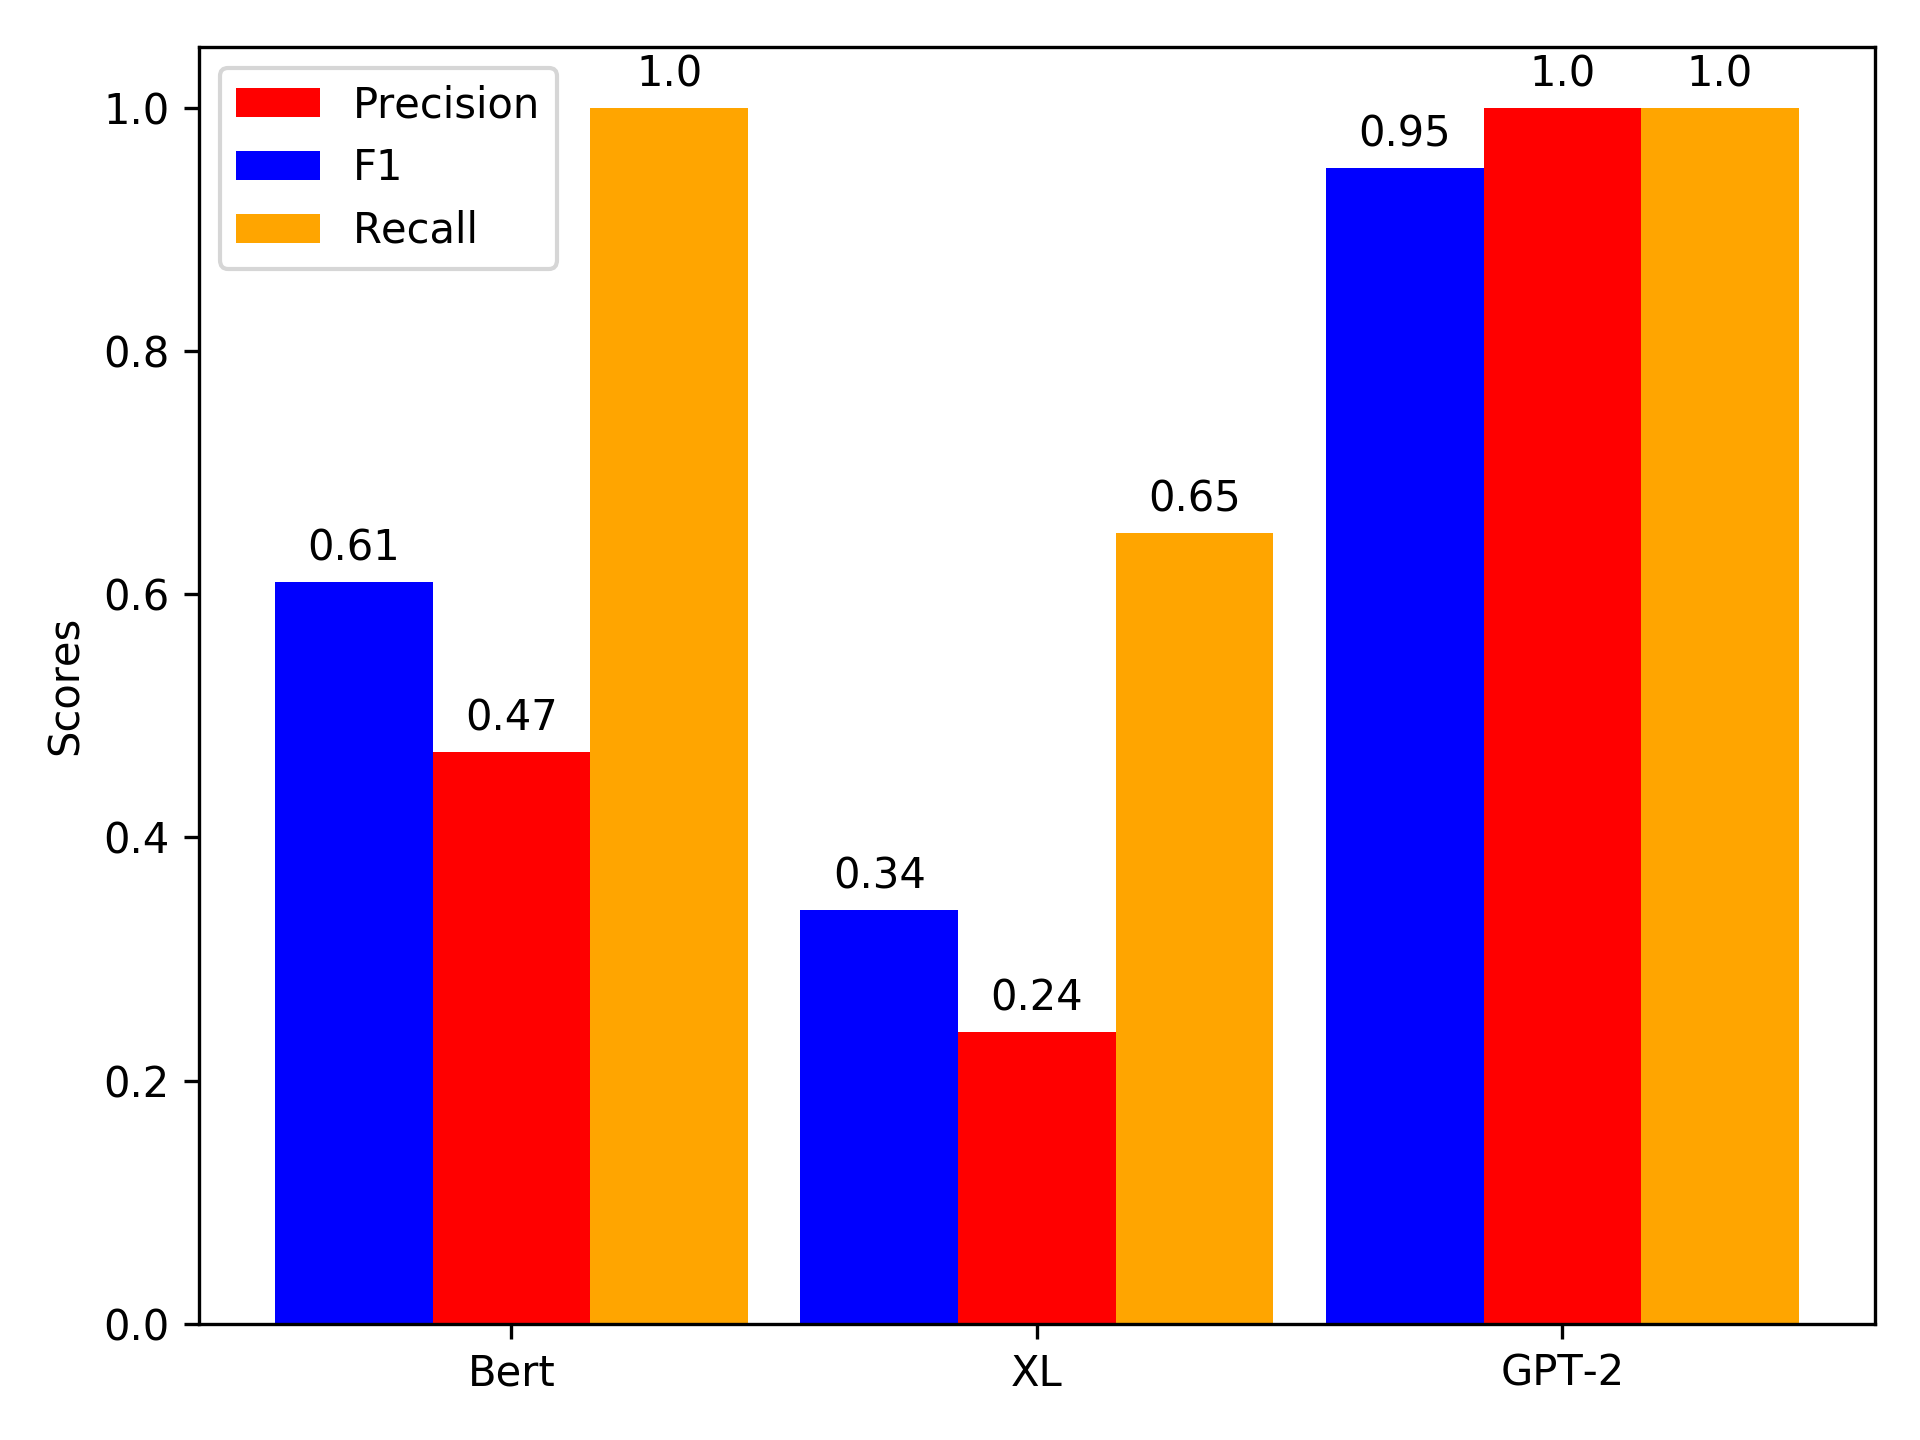
\includegraphics[trim={1cm 0.5cm 0cm 1cm}, width=0.322\textwidth]{results/average/regression_sequential_average_ratio_0.10.png}}
\hspace{\fill}
   \subfloat[15\% alteration\label{fig:results_regression_sequential_15}]{%
      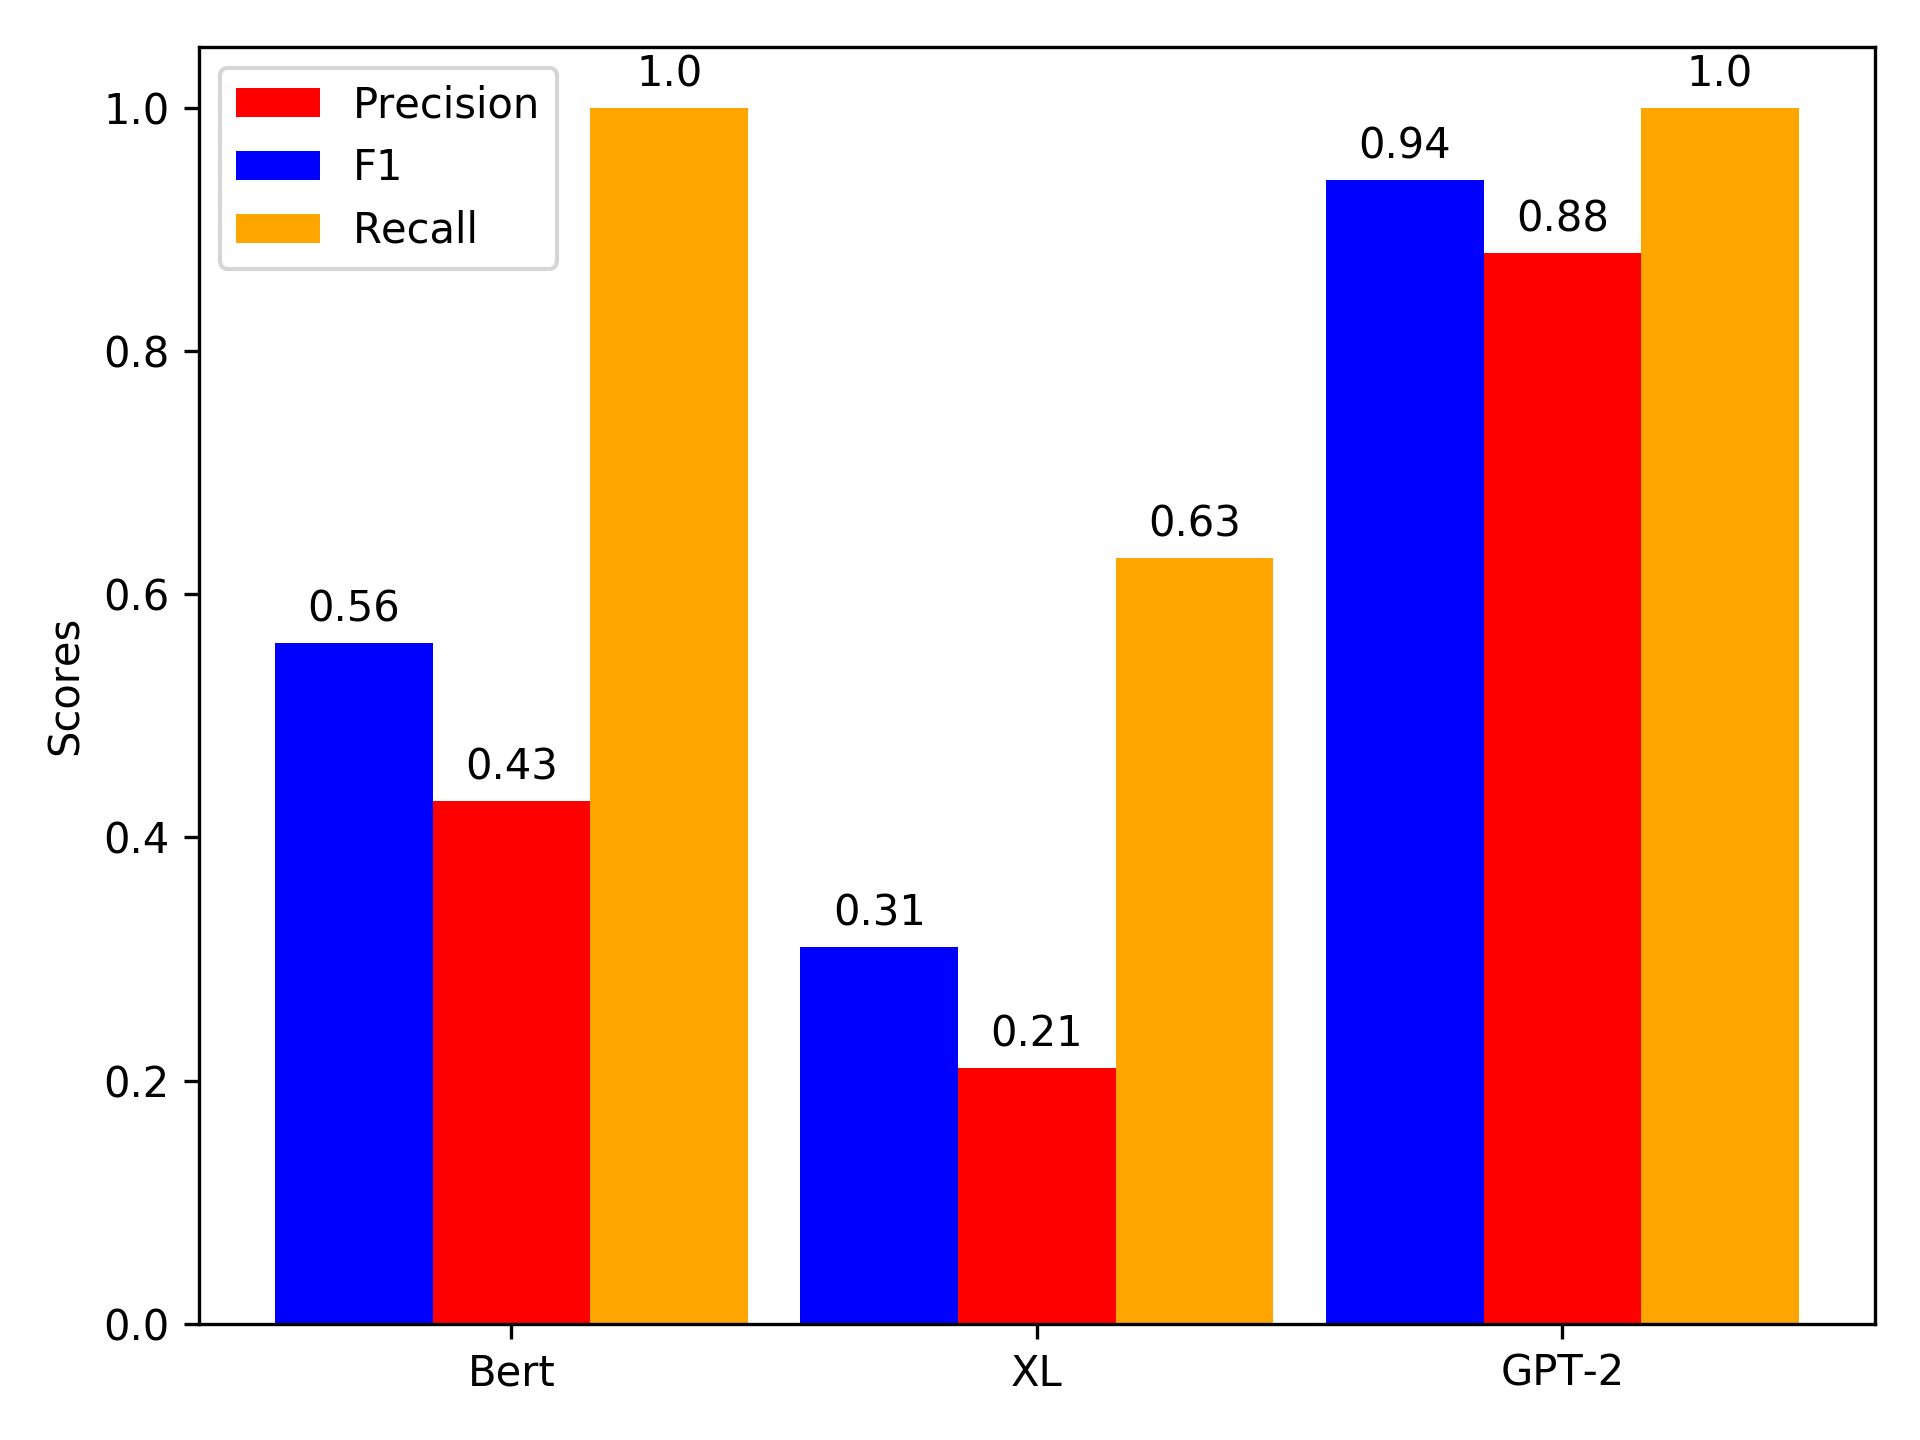
\includegraphics[trim={1cm 0.5cm 0cm 1cm}, width=0.322\textwidth]{results/average/regression_sequential_average_ratio_0.15.png}}\\
\caption{\label{fig:results_regression_sequential}Altering the sequences of logs at different ratios, using regression.}
\end{figure*}


\begin{figure*}[ht!]
  \centering
  \captionsetup{justification=centering}
   \subfloat[5\% alteration\label{fig:results_regression_qualitative_5}]{%
      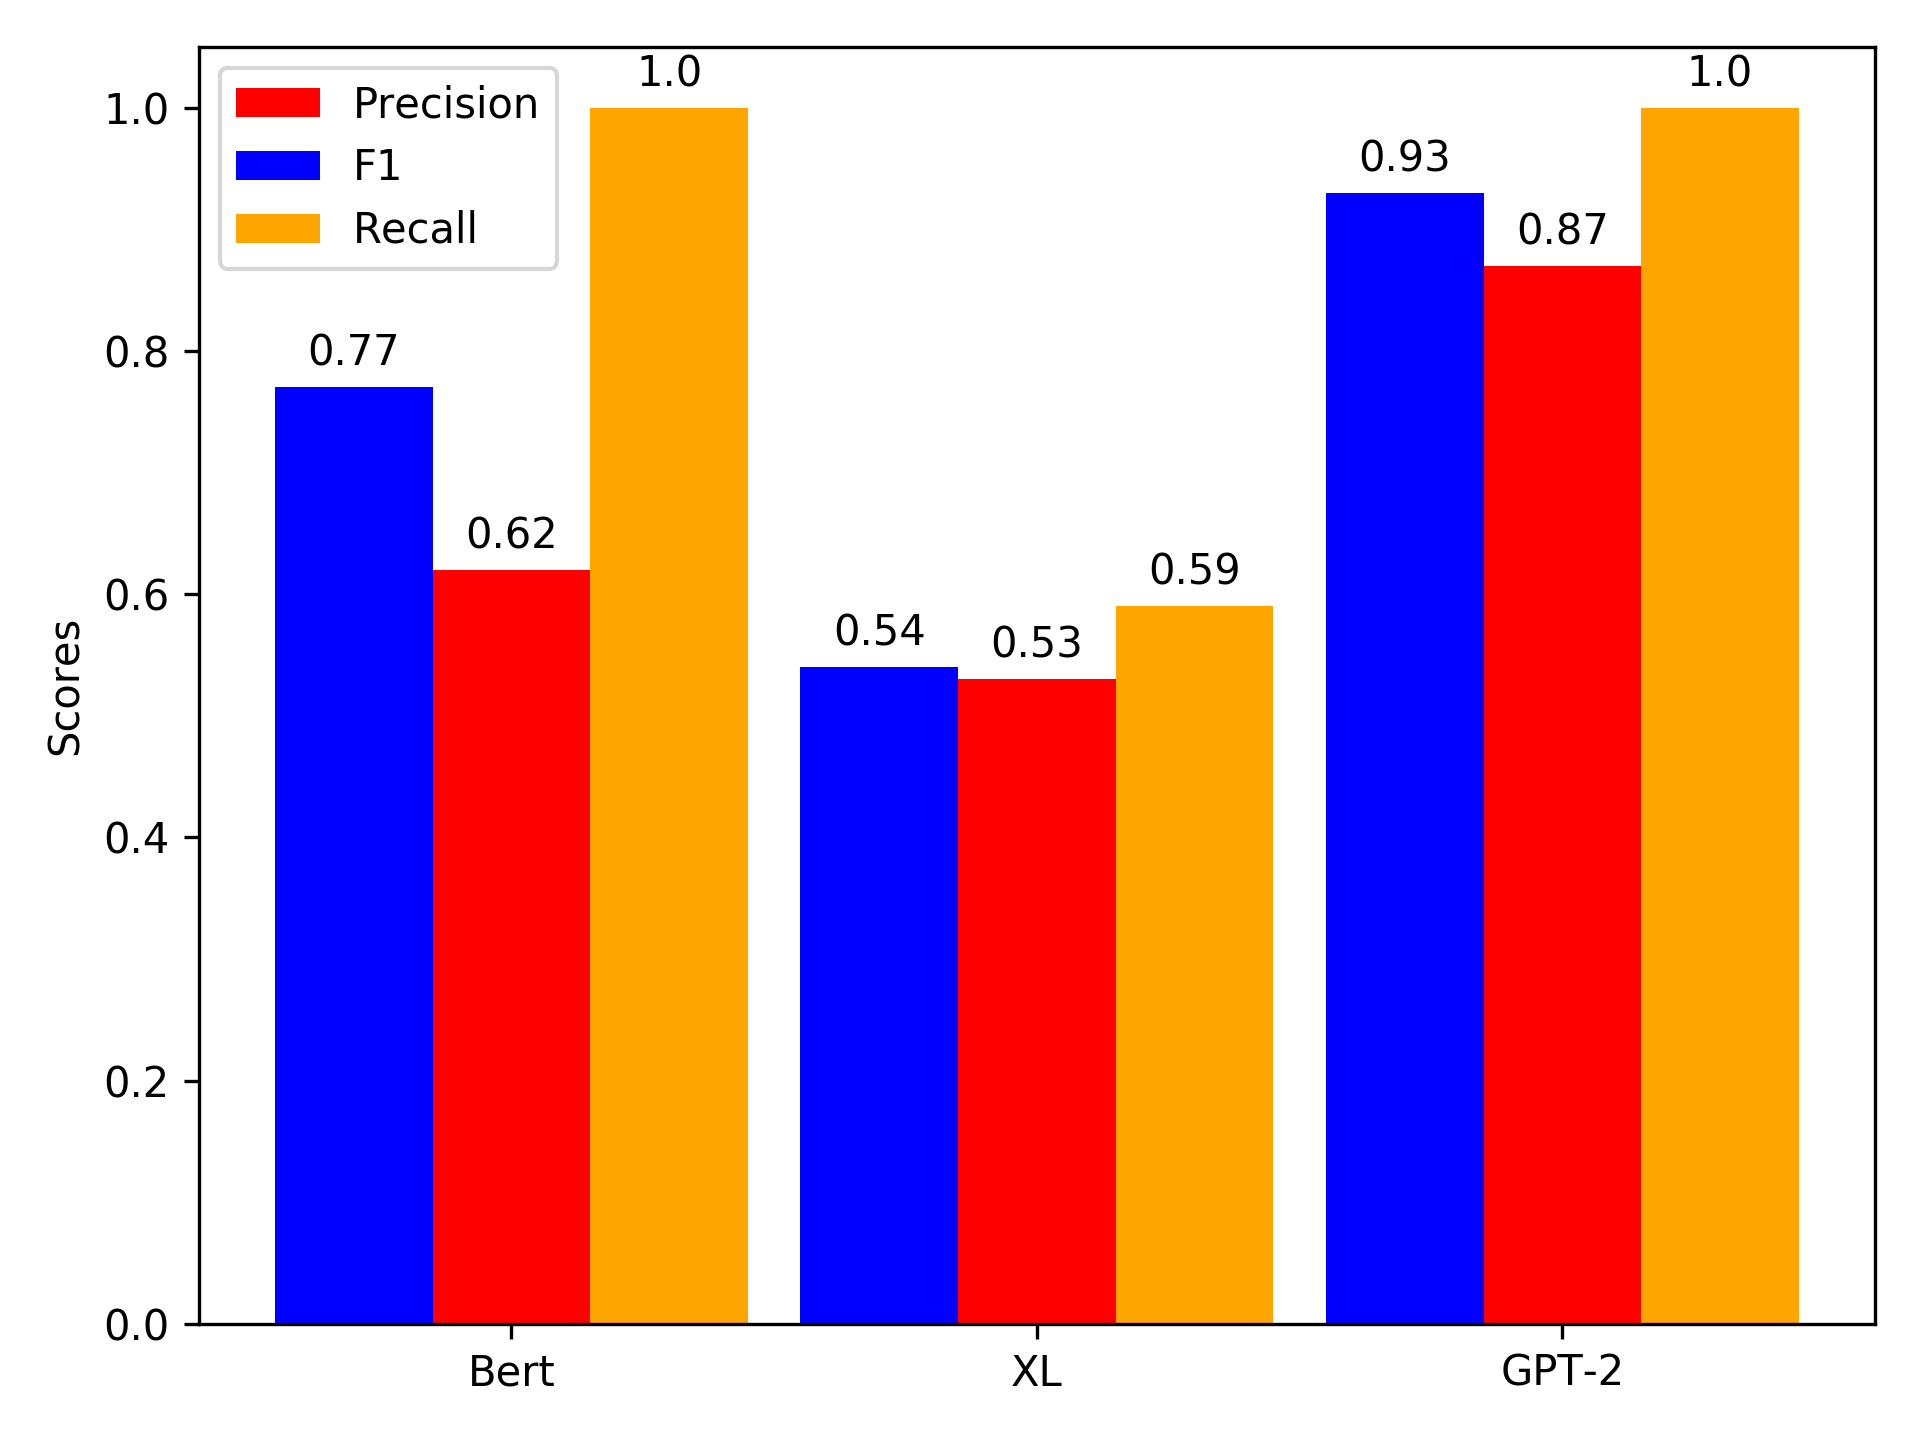
\includegraphics[trim={1cm 0.5cm 0cm 1cm}, width=0.322\textwidth]{results/average/regression_qualitative_average_ratio_0.05.png}}
\hspace{\fill}
   \subfloat[10\% alteration\label{fig:results_regression_qualitative_10} ]{%
      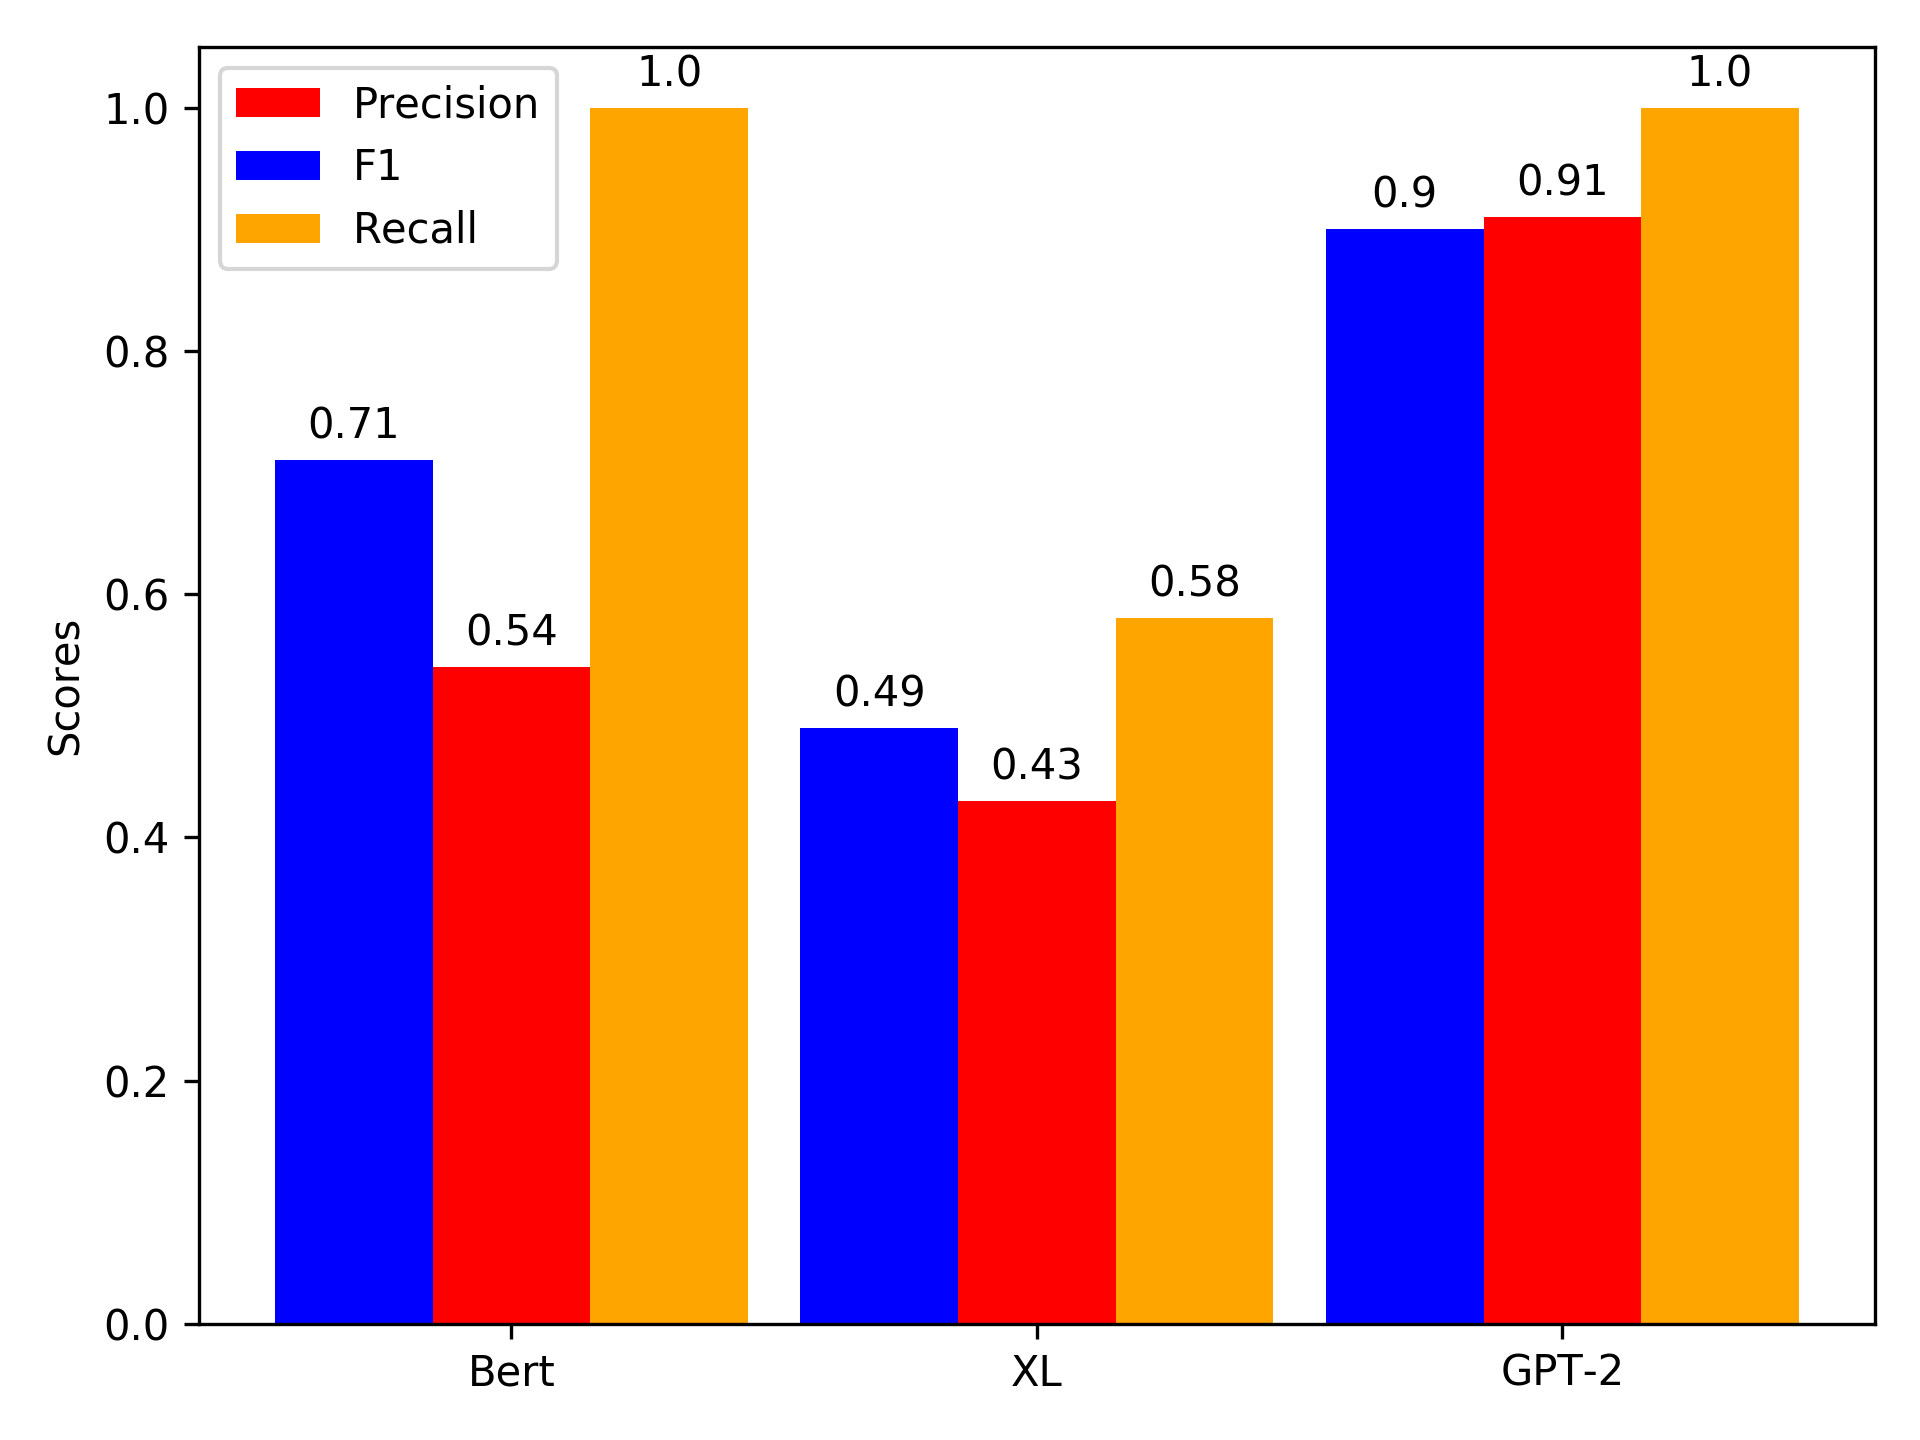
\includegraphics[trim={1cm 0.5cm 0cm 1cm}, width=0.322\textwidth]{results/average/regression_qualitative_average_ratio_0.10.png}}
\hspace{\fill}
   \subfloat[15\% alteration\label{fig:results_regression_qualitative_15}]{%
      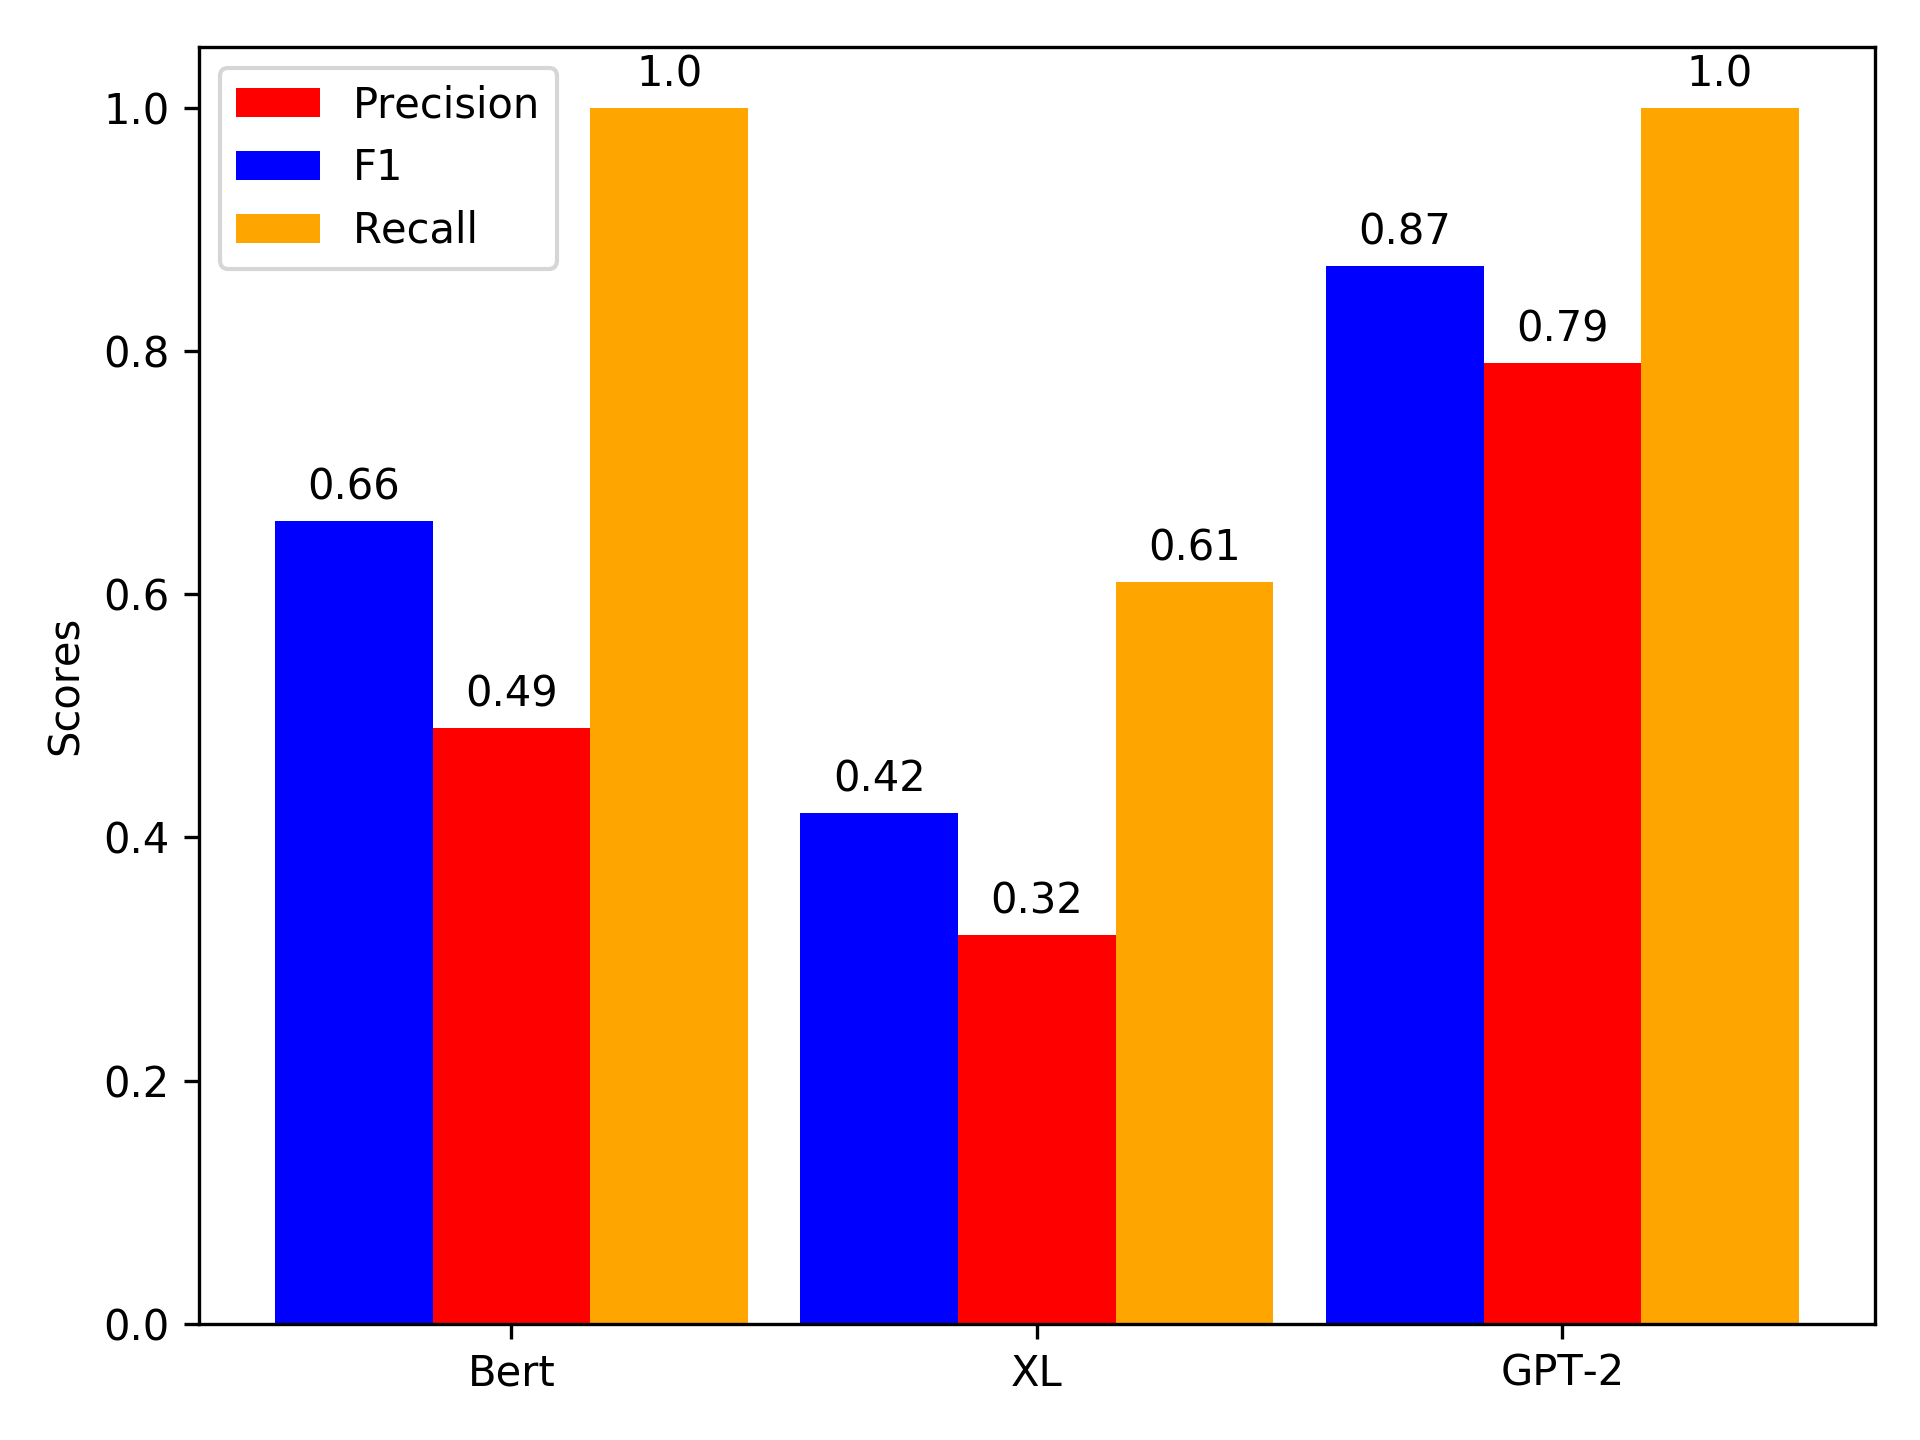
\includegraphics[trim={1cm 0.5cm 0cm 1cm}, width=0.322\textwidth]{results/average/regression_qualitative_average_ratio_0.15.png}}\\
\caption{\label{fig:results_regression_words}Altering log lines at different ratios, using regression.}
\end{figure*}	

%%%%%



\begin{figure}[h]
  \centering
  \captionsetup{justification=centering}
  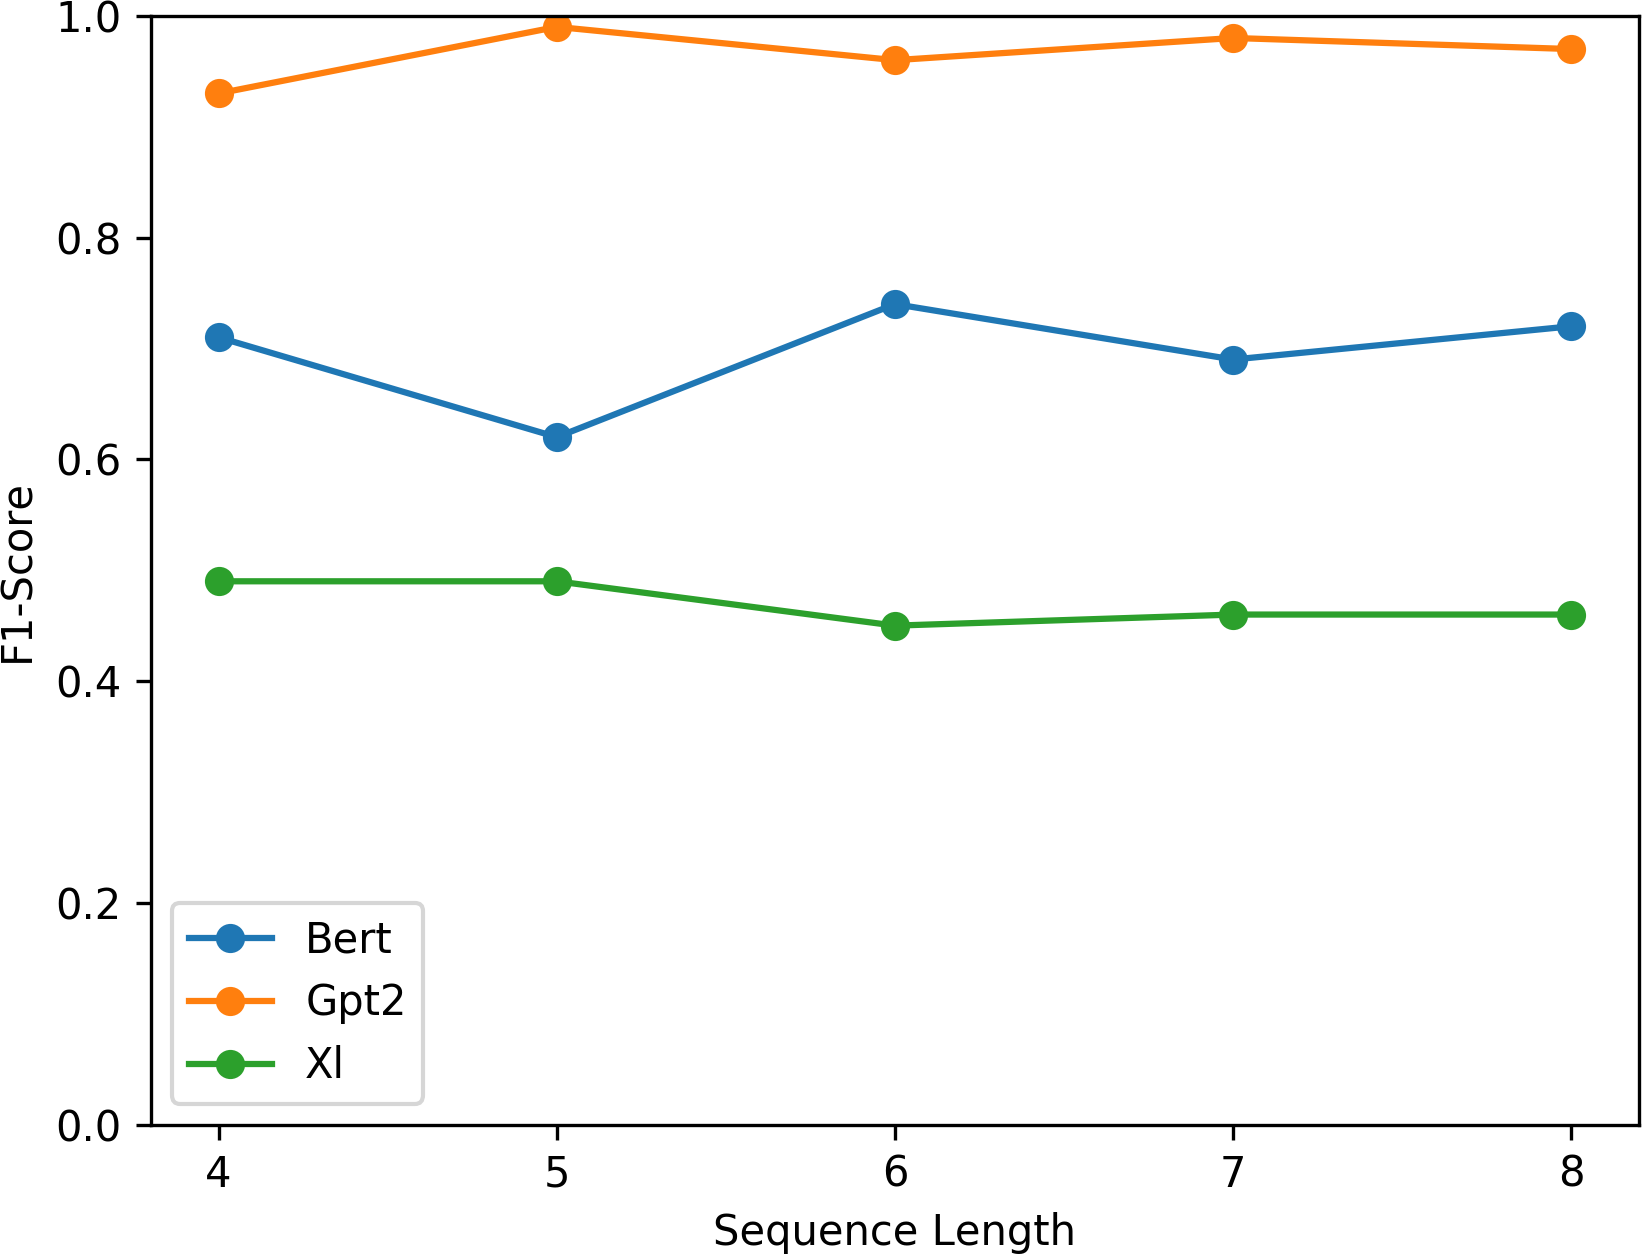
\includegraphics[width=9cm,height=6.5cm]{results/seq_len/sequence_len_regression.png}\\
  \caption{F1-Score for varying input sequence lengths, 15\% word insertion alterations, 5\% anomalies injected, using regression.}
  \label{fig:seq_len_regression}
\end{figure}





%%%%%%%%%%%%%%%%
% CLASSIFICATION 
%%%%%%%%%%%%%%%%
\subsection{Classification-based approach using one dataset \label{sec:results-classification}}
In this subsection, the results of the classification-based approach are presented, with the exact same boundary conditions as in \ref{sec:results-regression}. 
The ability of the system to detect injected anomalies, despite injected alterations on the sequences of logs, can be seen in \ref{fig:results_multiclass_sequential}. 
The impact of alterations on the sequence of logs, i.e. deleting, shuffling and duplicating events are summarised in figure \ref{fig:results_regression_sequential}. Again, only average results on the individual injections are presented. Results broken down by each alteration can be found in the appendix \ref{appendix:classification}. 

In contrary to the results using regression, the classification approach seems most fit for Bert and much less for GPT-2. This is probably due to the smaller cosine distance between the templates in GPT-2, which makes it harder for the system to correctly assign the templates to the classes in the prediction process.

Additionally to the alterations on the log sequences, the results alterations on the log events themselves, i.e. inserting, removing and replacing words are of interest. The results of this experiment can be seen in figure \ref{fig:results_multiclass_sequential}. Again, the alterations are not injected all at once, but independently - the figure shows averaged results.

The impact of the input sequence length can be seen in \ref{fig:seq_len_regression}. Bert again seems to profit slightly from sequence lengths longer than 6 or 7, whereas the quality of results for XL-Transformers and GPT-2 seem to have a tendency to degrade in prediction quality for longer input sequence lengths.


%\begin{figure}[h]
%  \centering
%  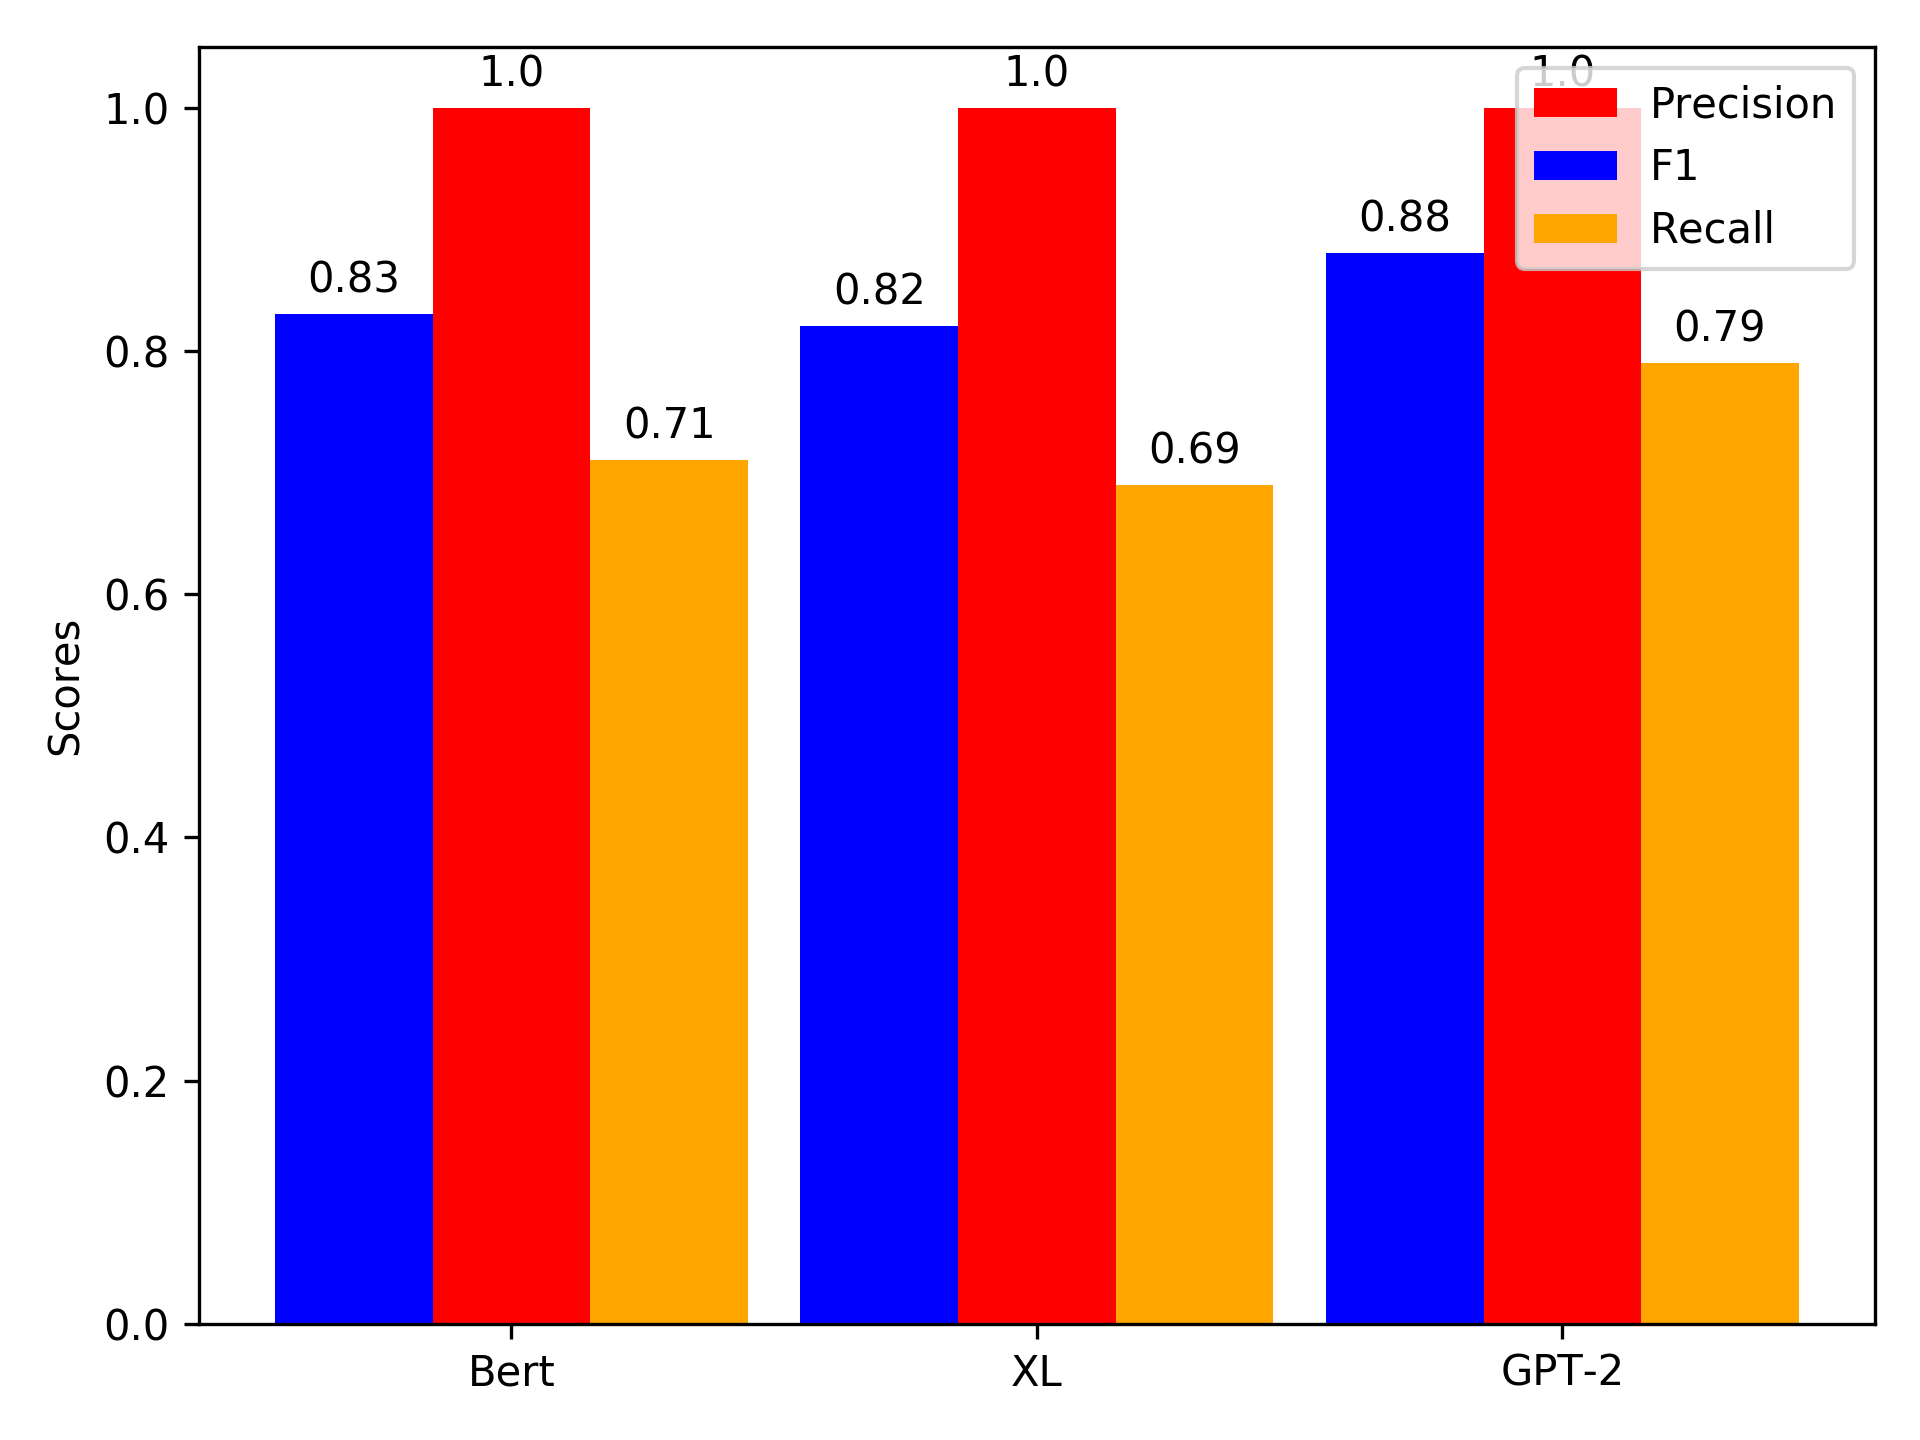
\includegraphics[width=6cm,height=4.5cm]{results/classification_sequence/multiclass_reverse.png}\\
%  \caption{Scores for detecting reversed order of log events, using classification.}
%  \label{fig:multiclass_reverse_order}
%\end{figure}
% multiclass sequential
\begin{figure*}[ht!]
  \centering
  \captionsetup{justification=centering}
   \subfloat[5\% alteration\label{fig:results_multiclass_sequential_5}]{%
      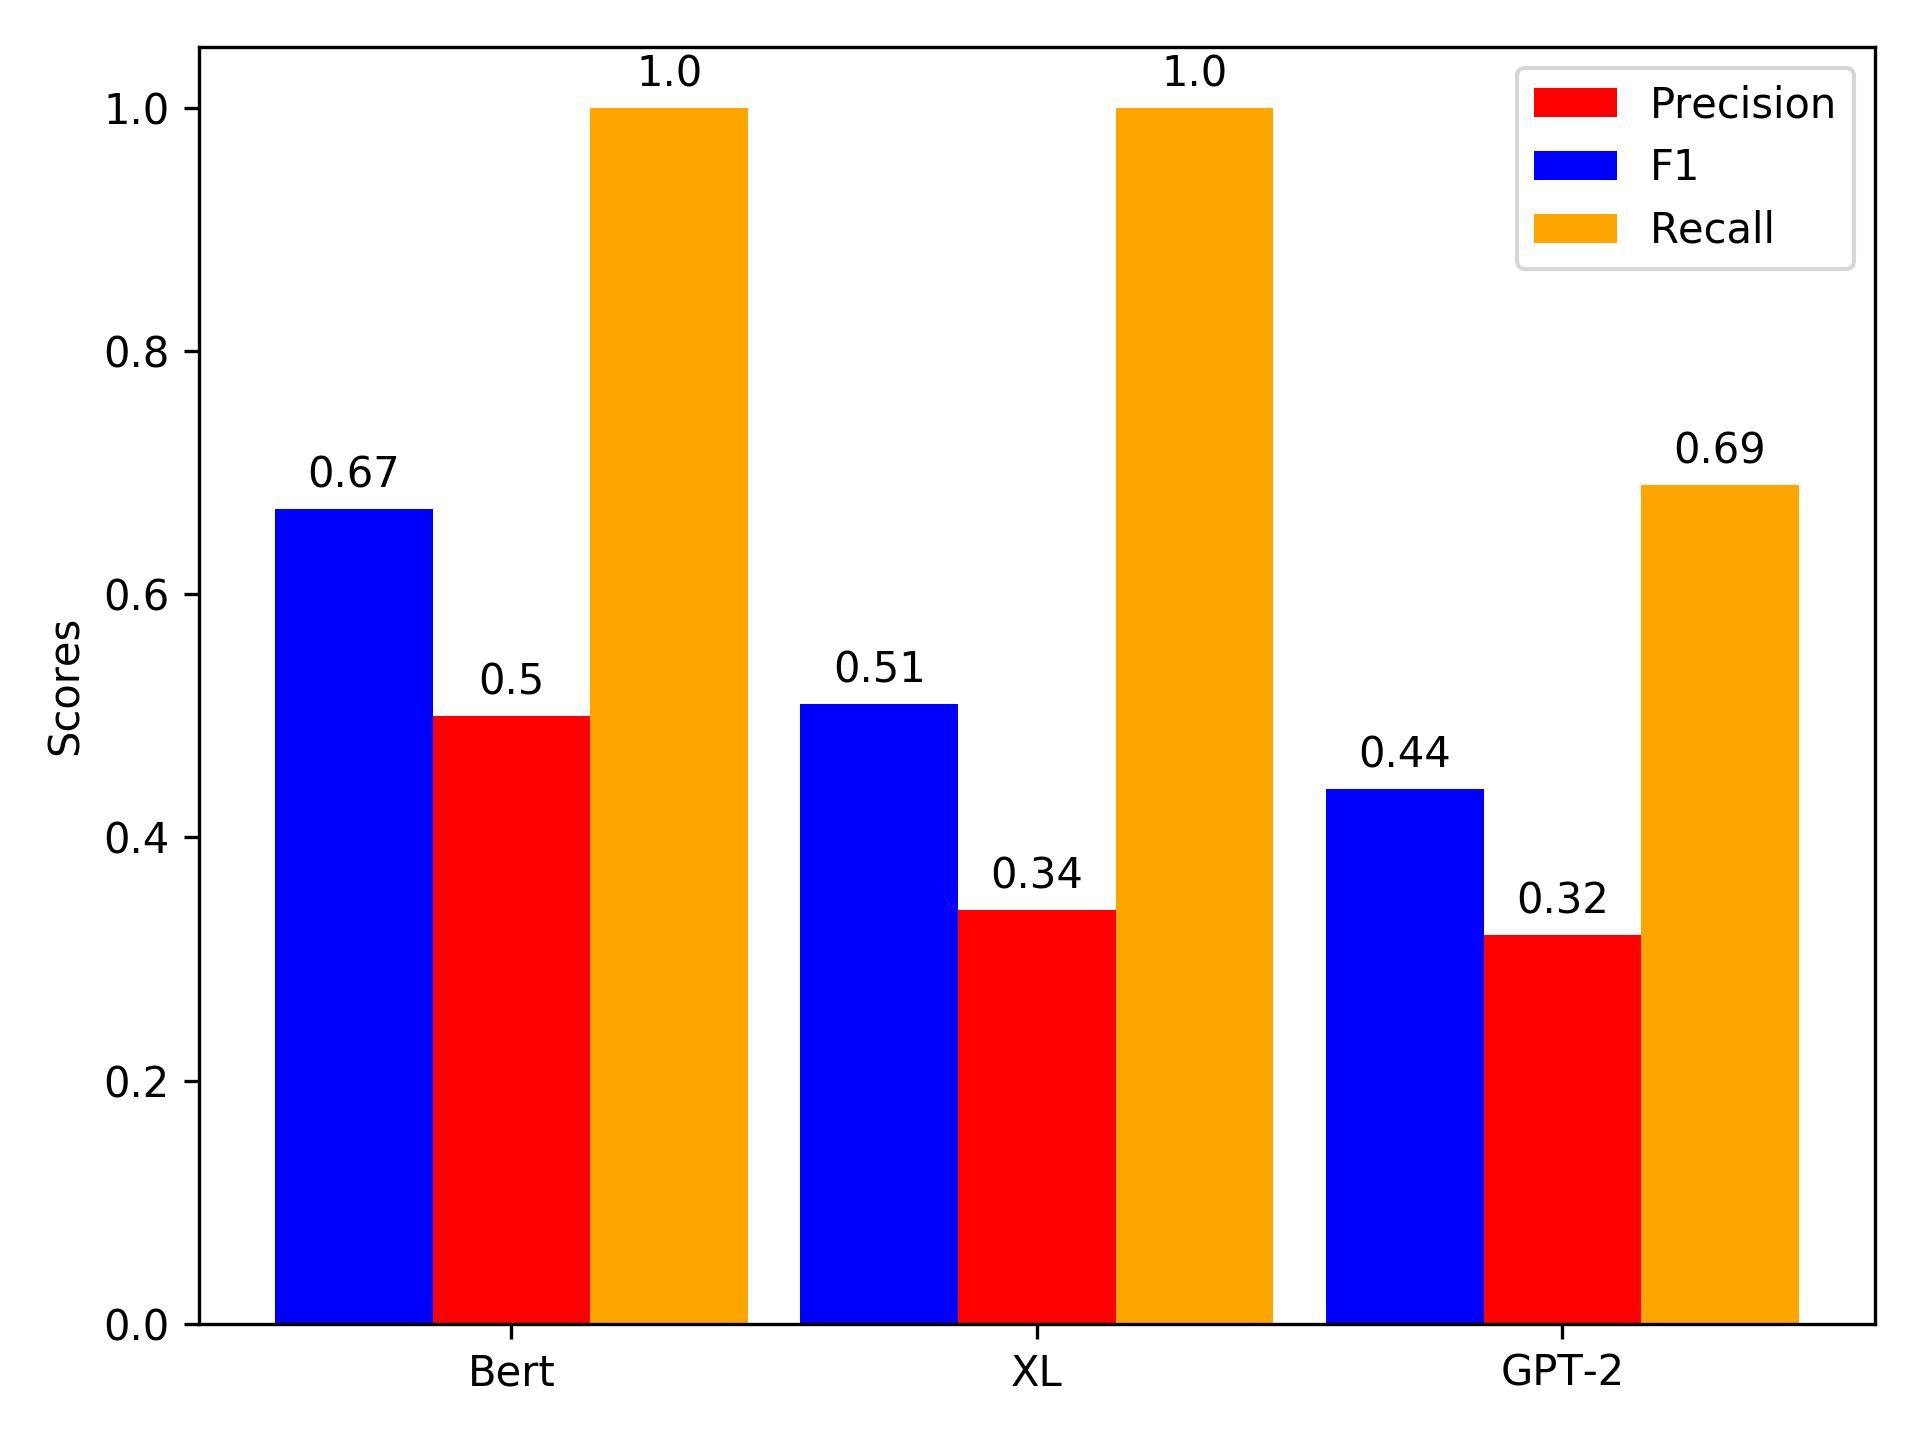
\includegraphics[trim={1cm 0.5cm 0cm 1cm}, width=0.322\textwidth]{results/average/multiclass_sequential_average_ratio_0.05.png}}
\hspace{\fill}
   \subfloat[10\% alteration\label{fig:results_multiclass_sequential_10} ]{%
      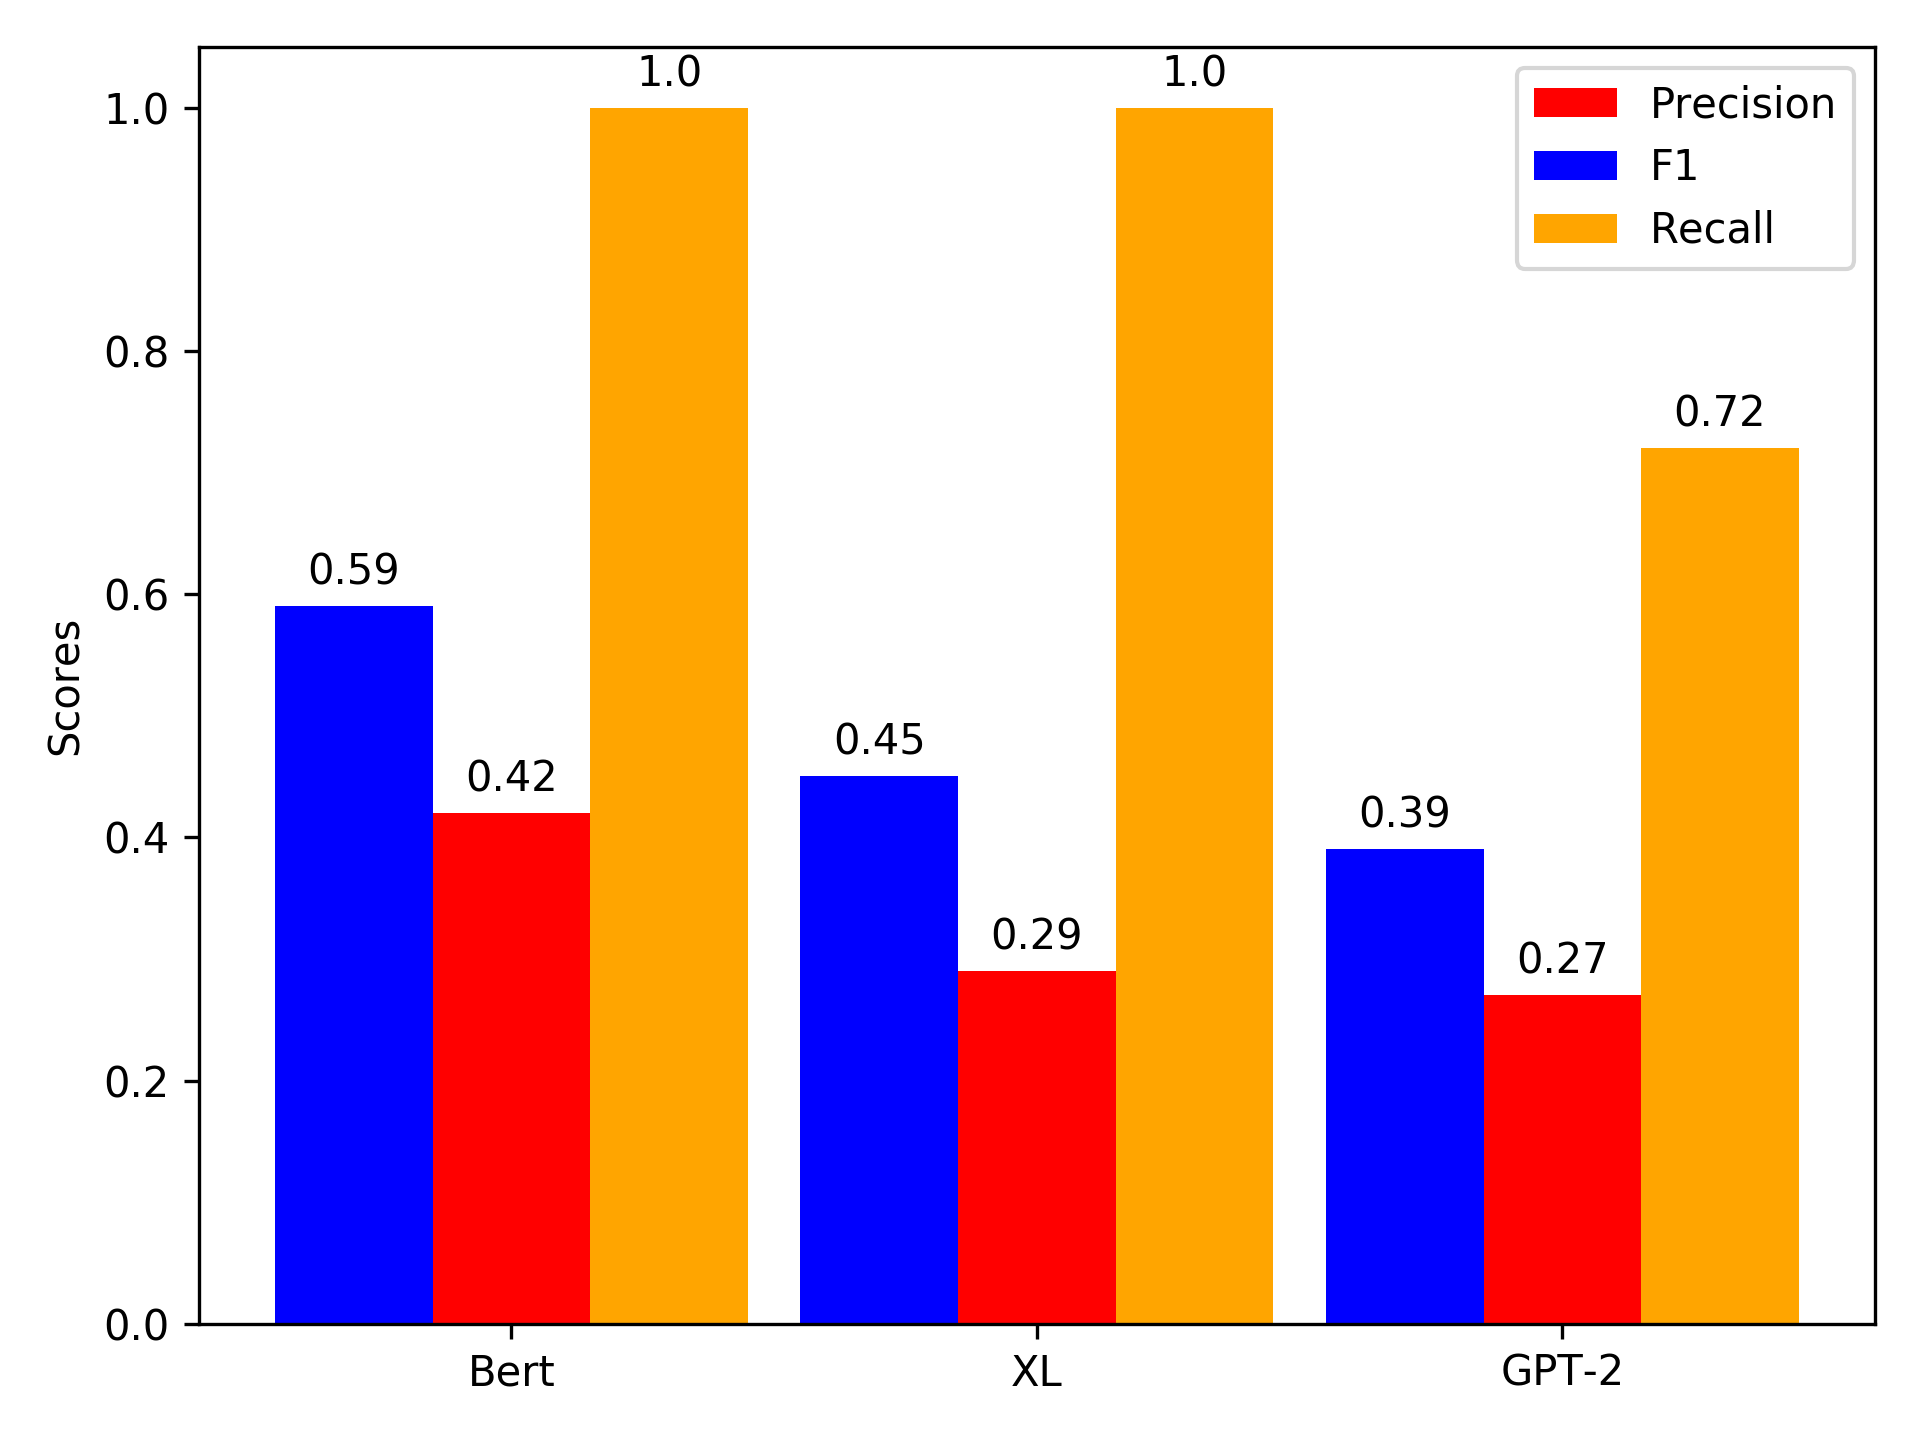
\includegraphics[trim={1cm 0.5cm 0cm 1cm}, width=0.322\textwidth]{results/average/multiclass_sequential_average_ratio_0.10.png}}
\hspace{\fill}
   \subfloat[15\% alteration\label{fig:results_multiclass_sequential_15}]{%
      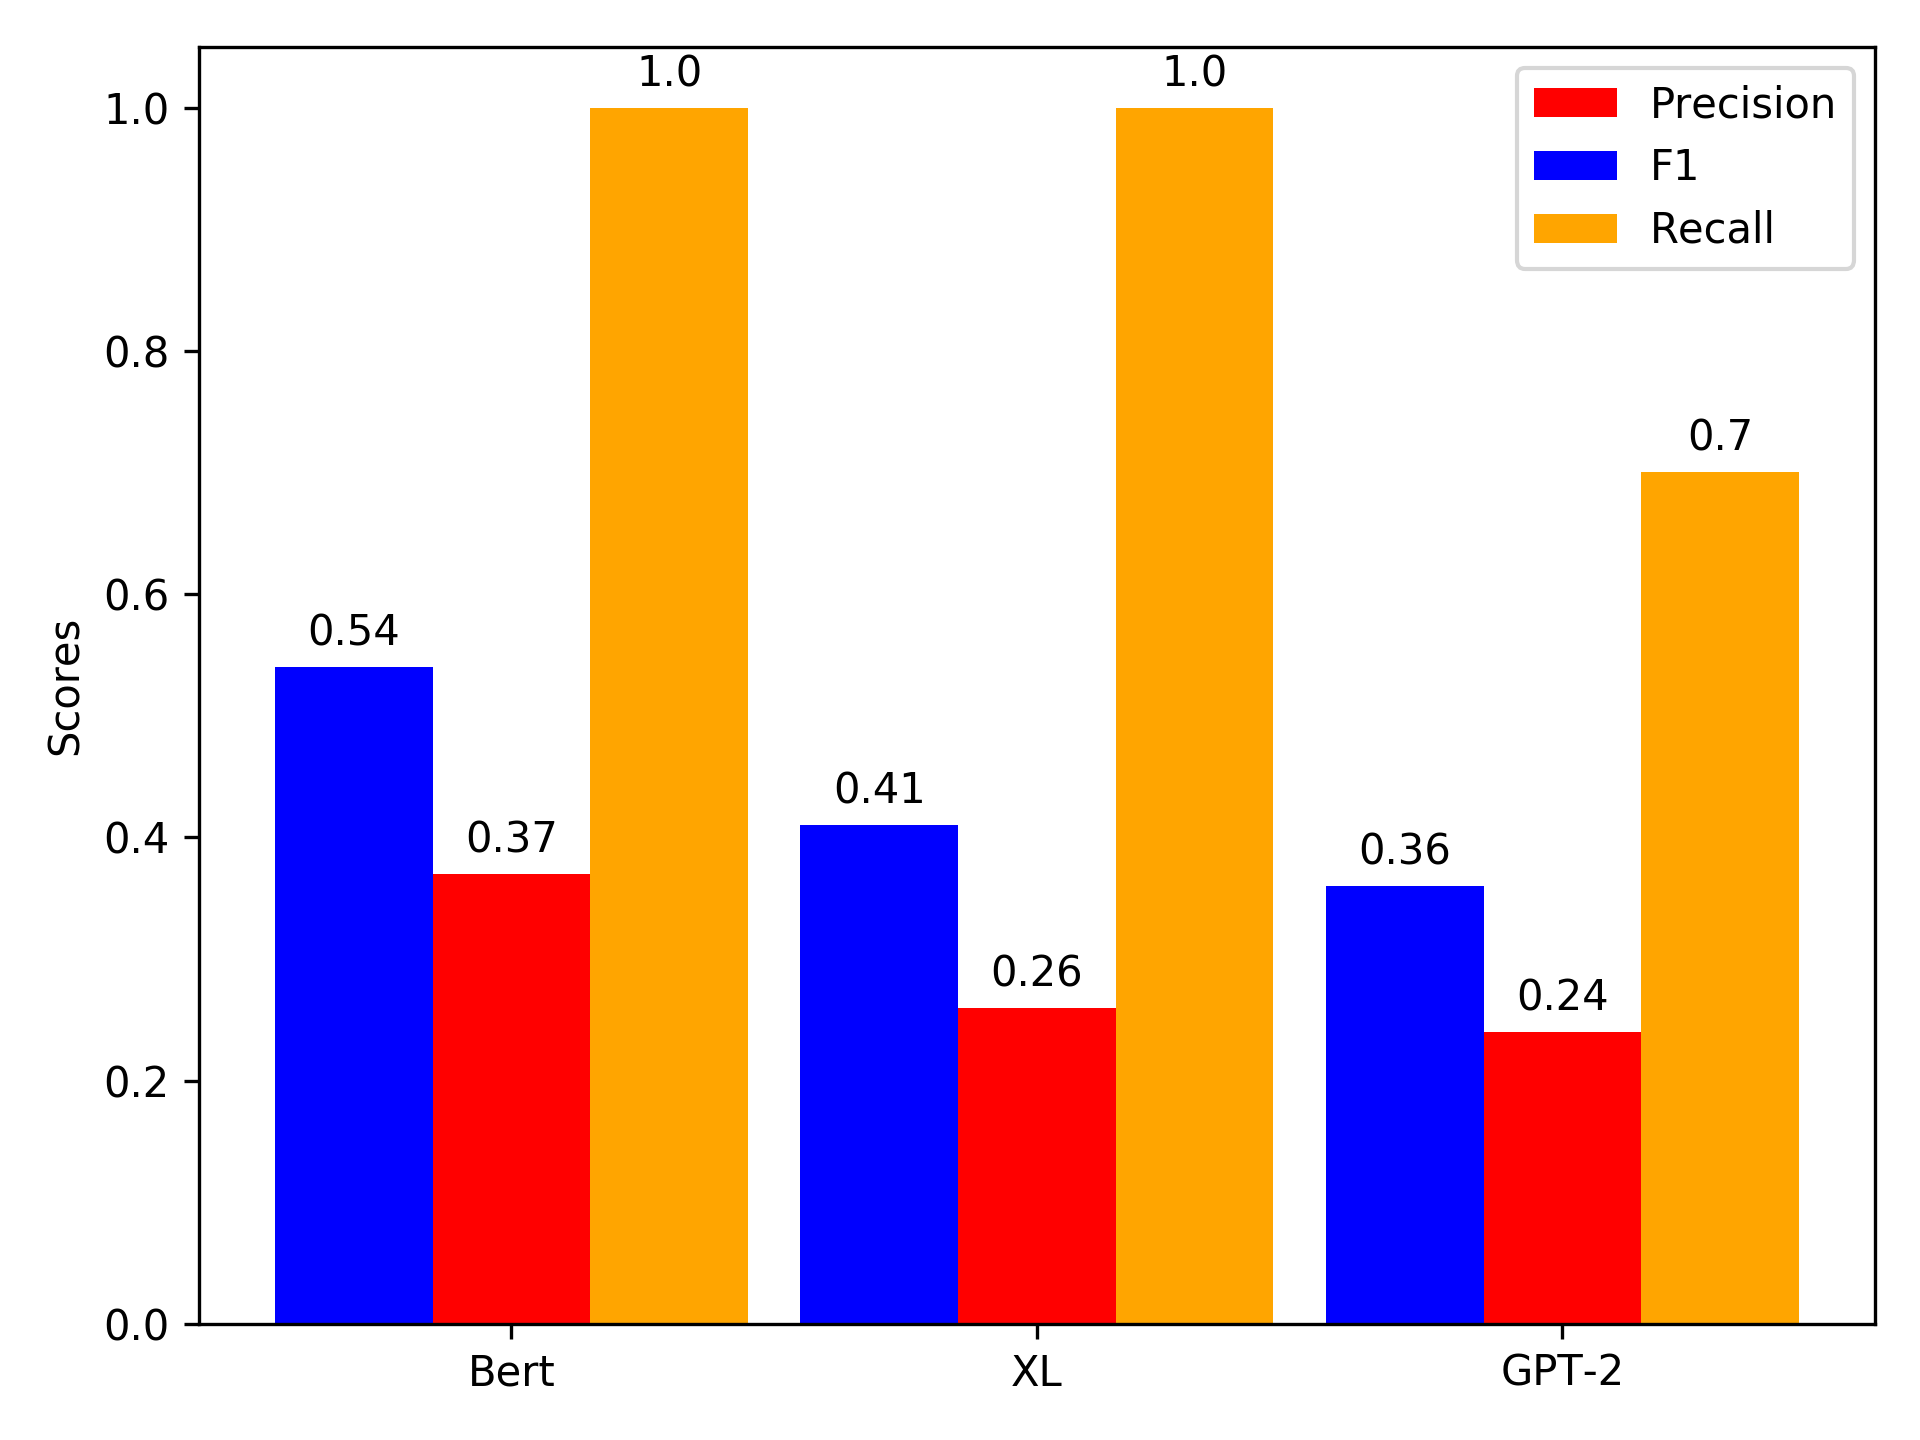
\includegraphics[trim={1cm 0.5cm 0cm 1cm}, width=0.322\textwidth]{results/average/multiclass_sequential_average_ratio_0.15.png}}\\
\caption{\label{fig:results_multiclass_sequential}Altering the order of log sequences at different ratios, using classification.}
\end{figure*}

%multiclass qualitative
\begin{figure*}[ht!]
  \centering
  \captionsetup{justification=centering}
   \subfloat[5\% alteration\label{fig:results_multiclass_qualitative_5}]{%
      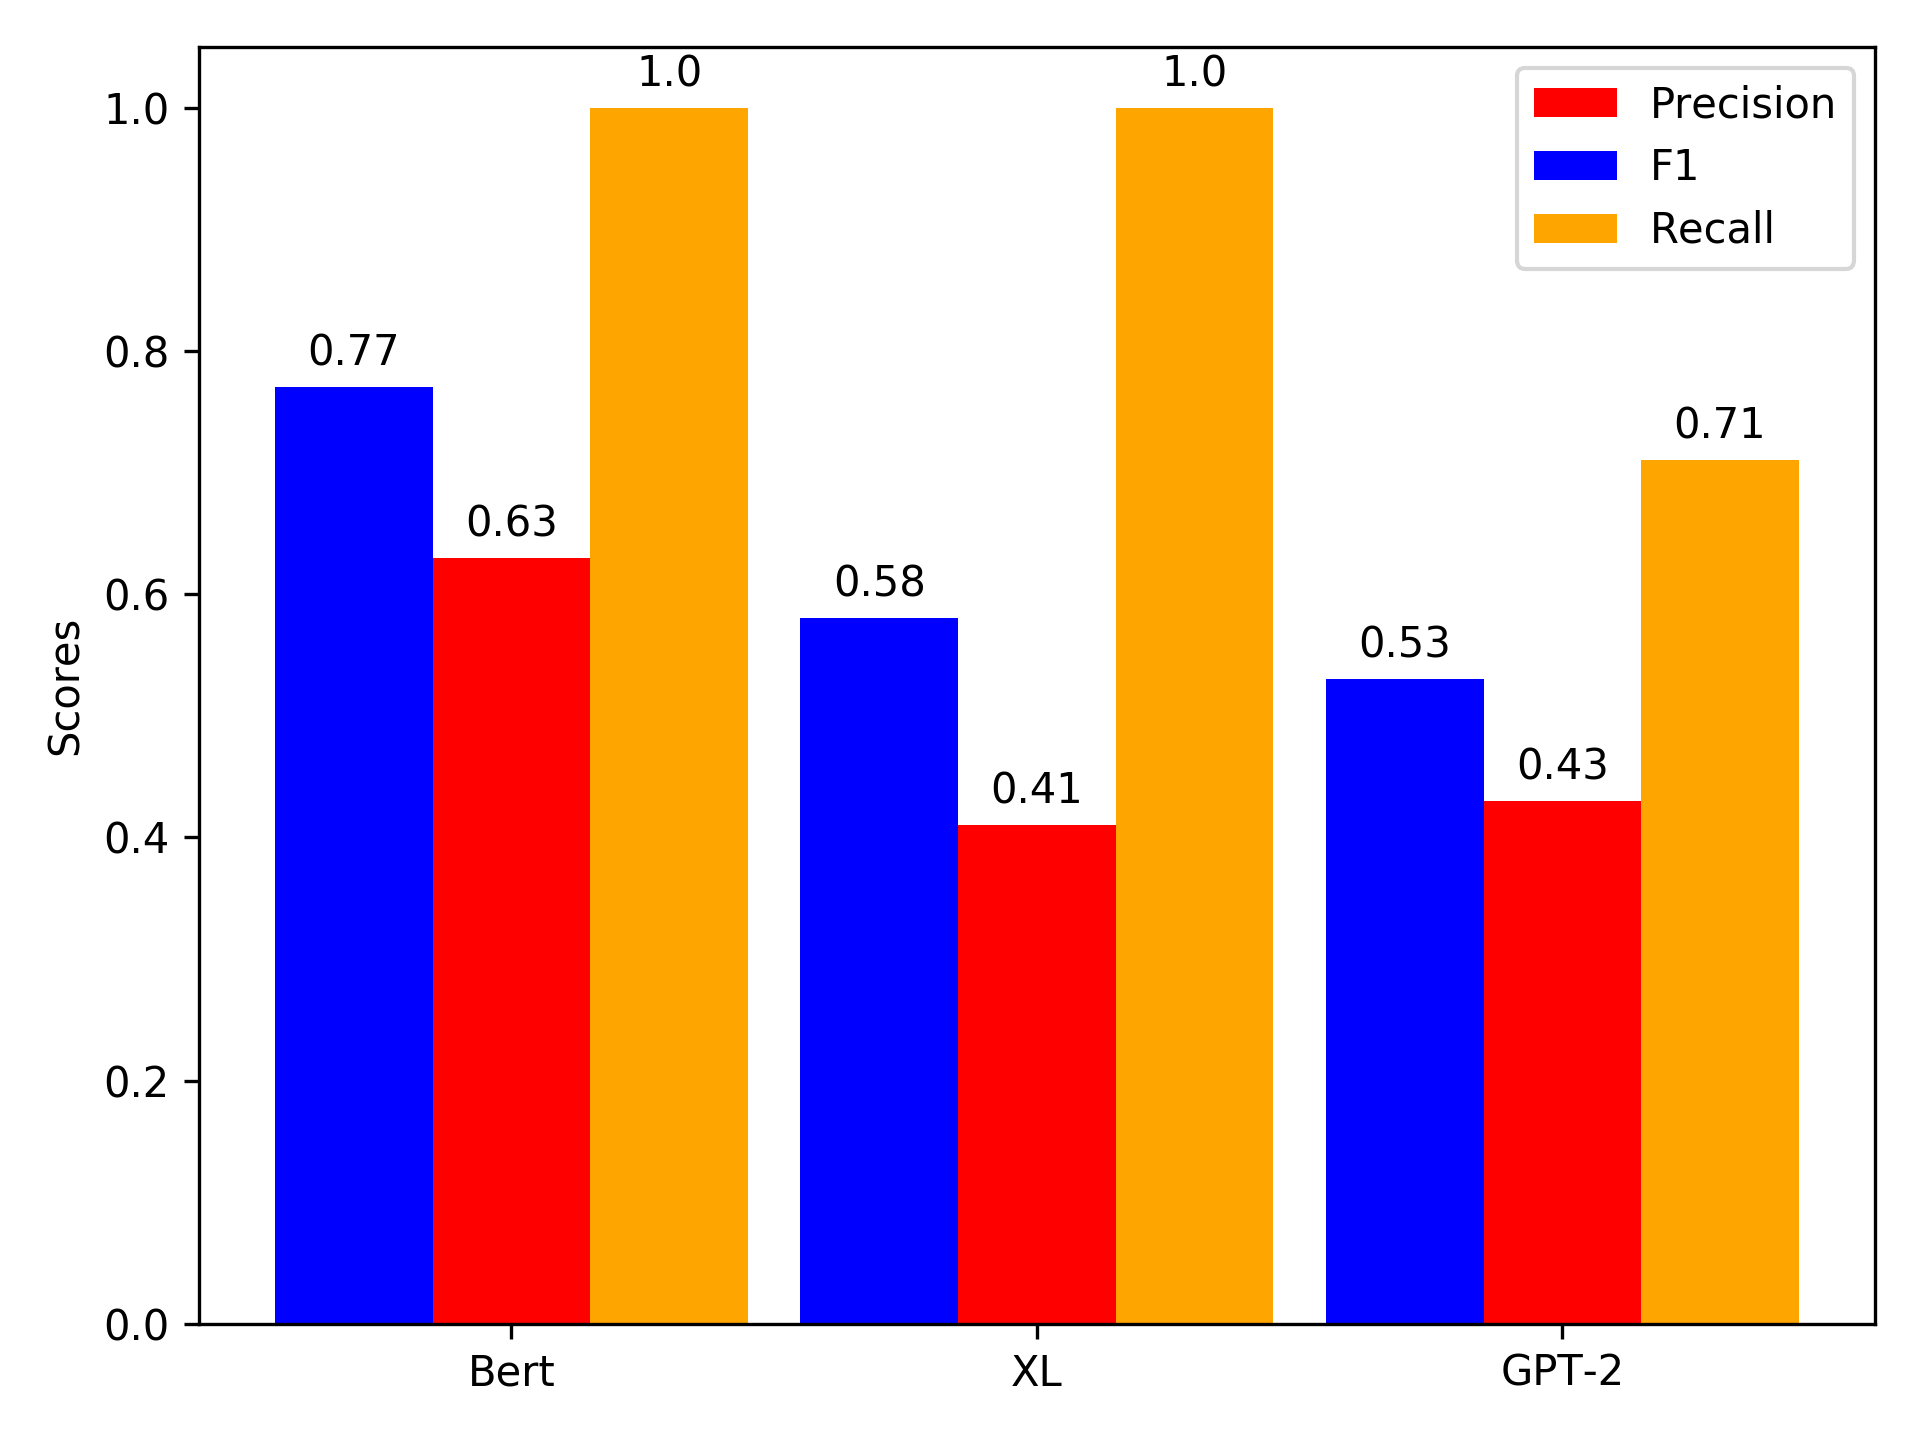
\includegraphics[trim={1cm 0.5cm 0cm 1cm}, width=0.322\textwidth]{results/average/multiclass_qualitative_average_ratio_0.05.png}}
\hspace{\fill}
   \subfloat[10\% alteration\label{fig:results_multiclass_qualitative_10} ]{%
      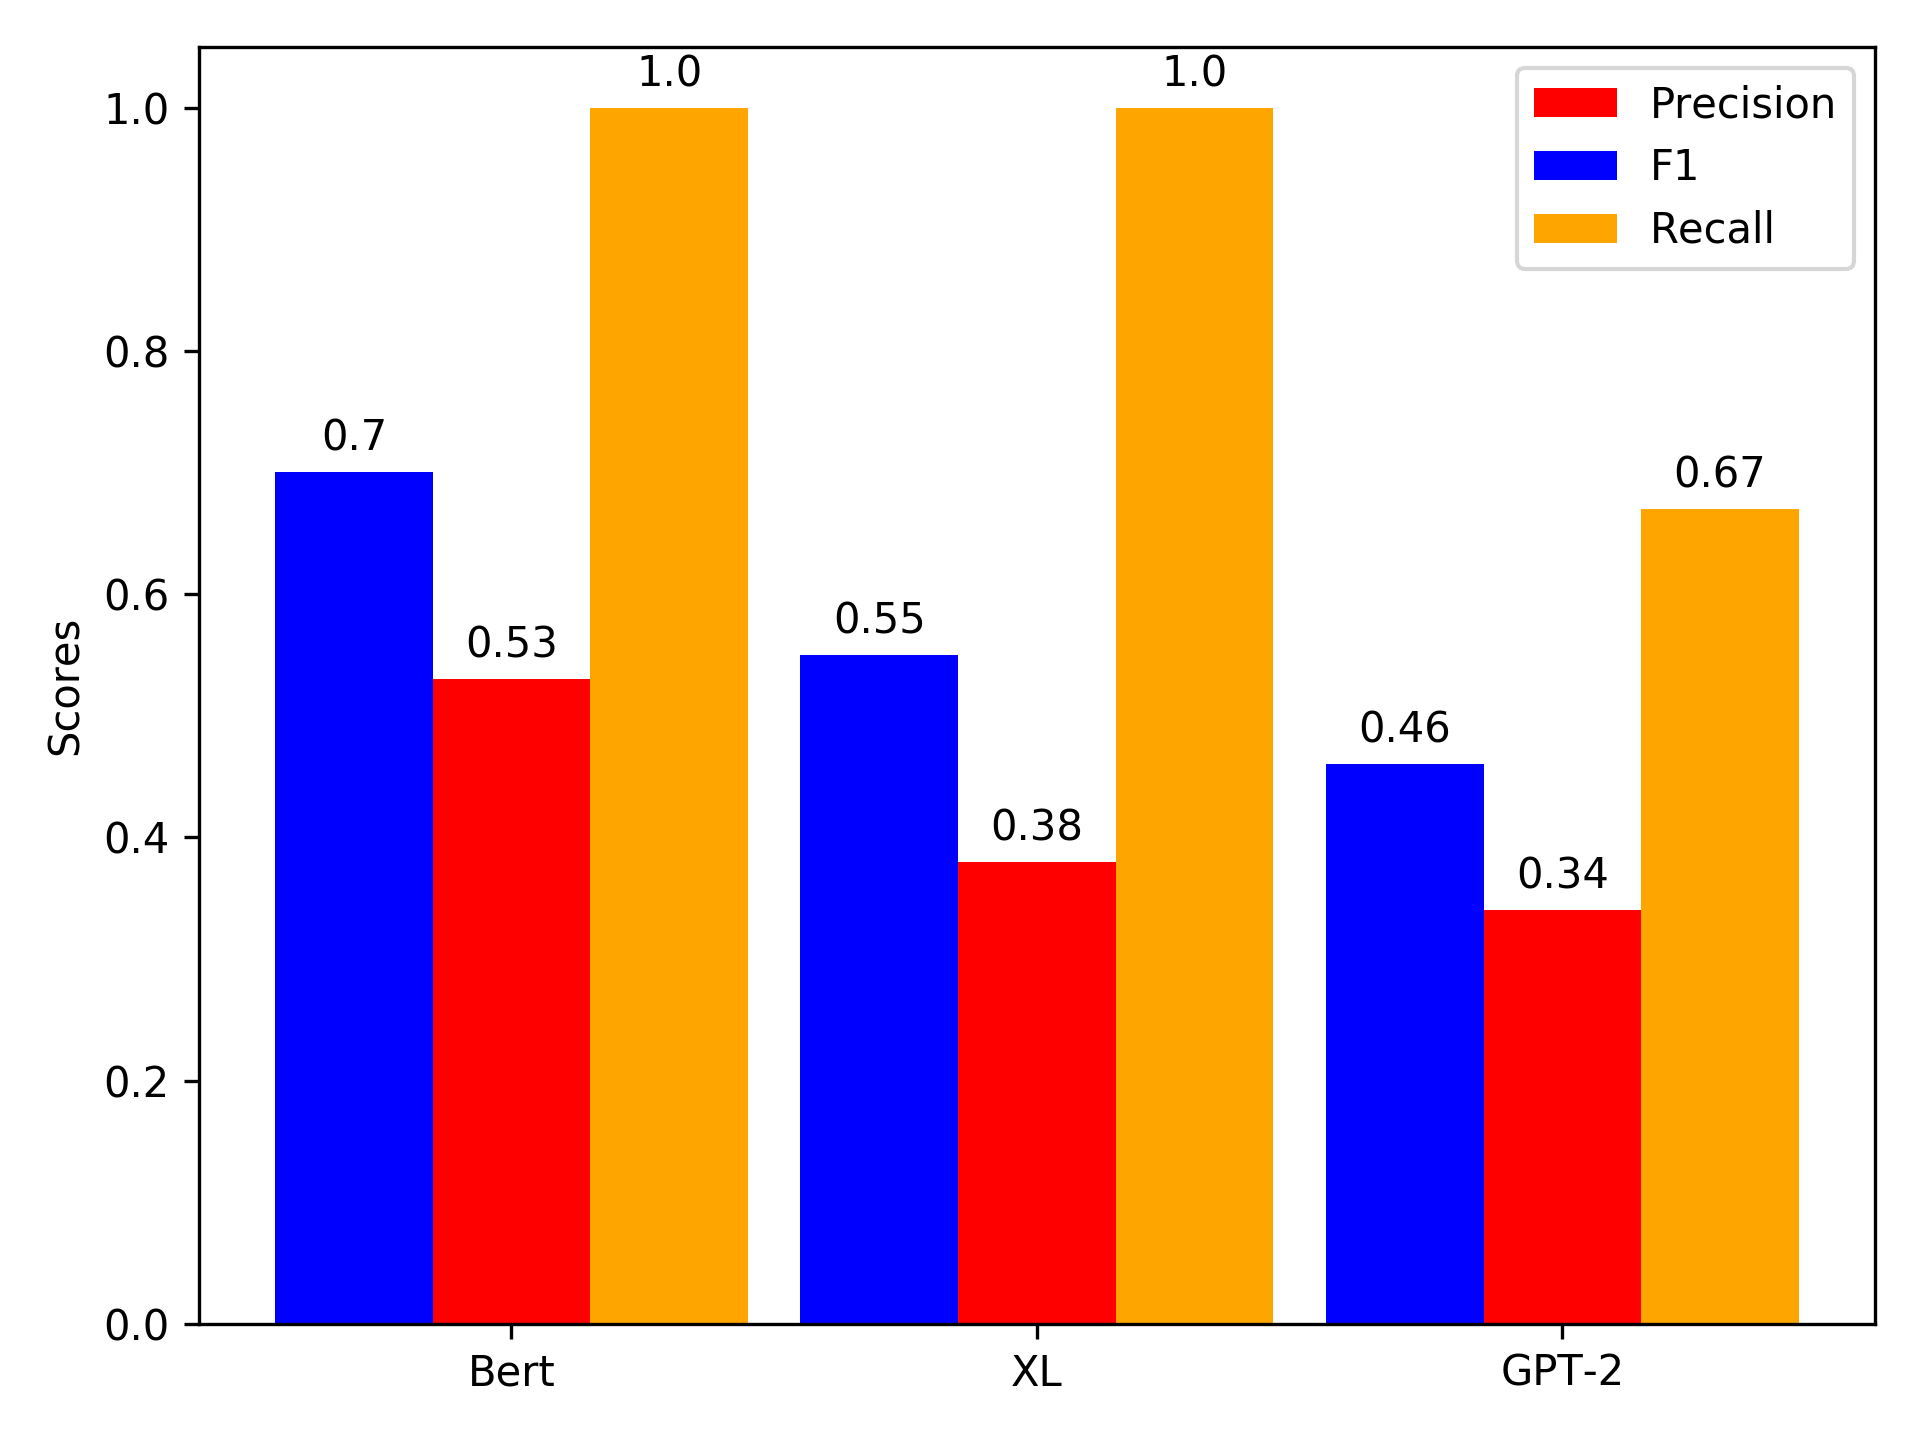
\includegraphics[trim={1cm 0.5cm 0cm 1cm}, width=0.322\textwidth]{results/average/multiclass_qualitative_average_ratio_0.10.png}}
\hspace{\fill}
   \subfloat[15\% alteration\label{fig:results_multiclass_qualitative_15}]{%
      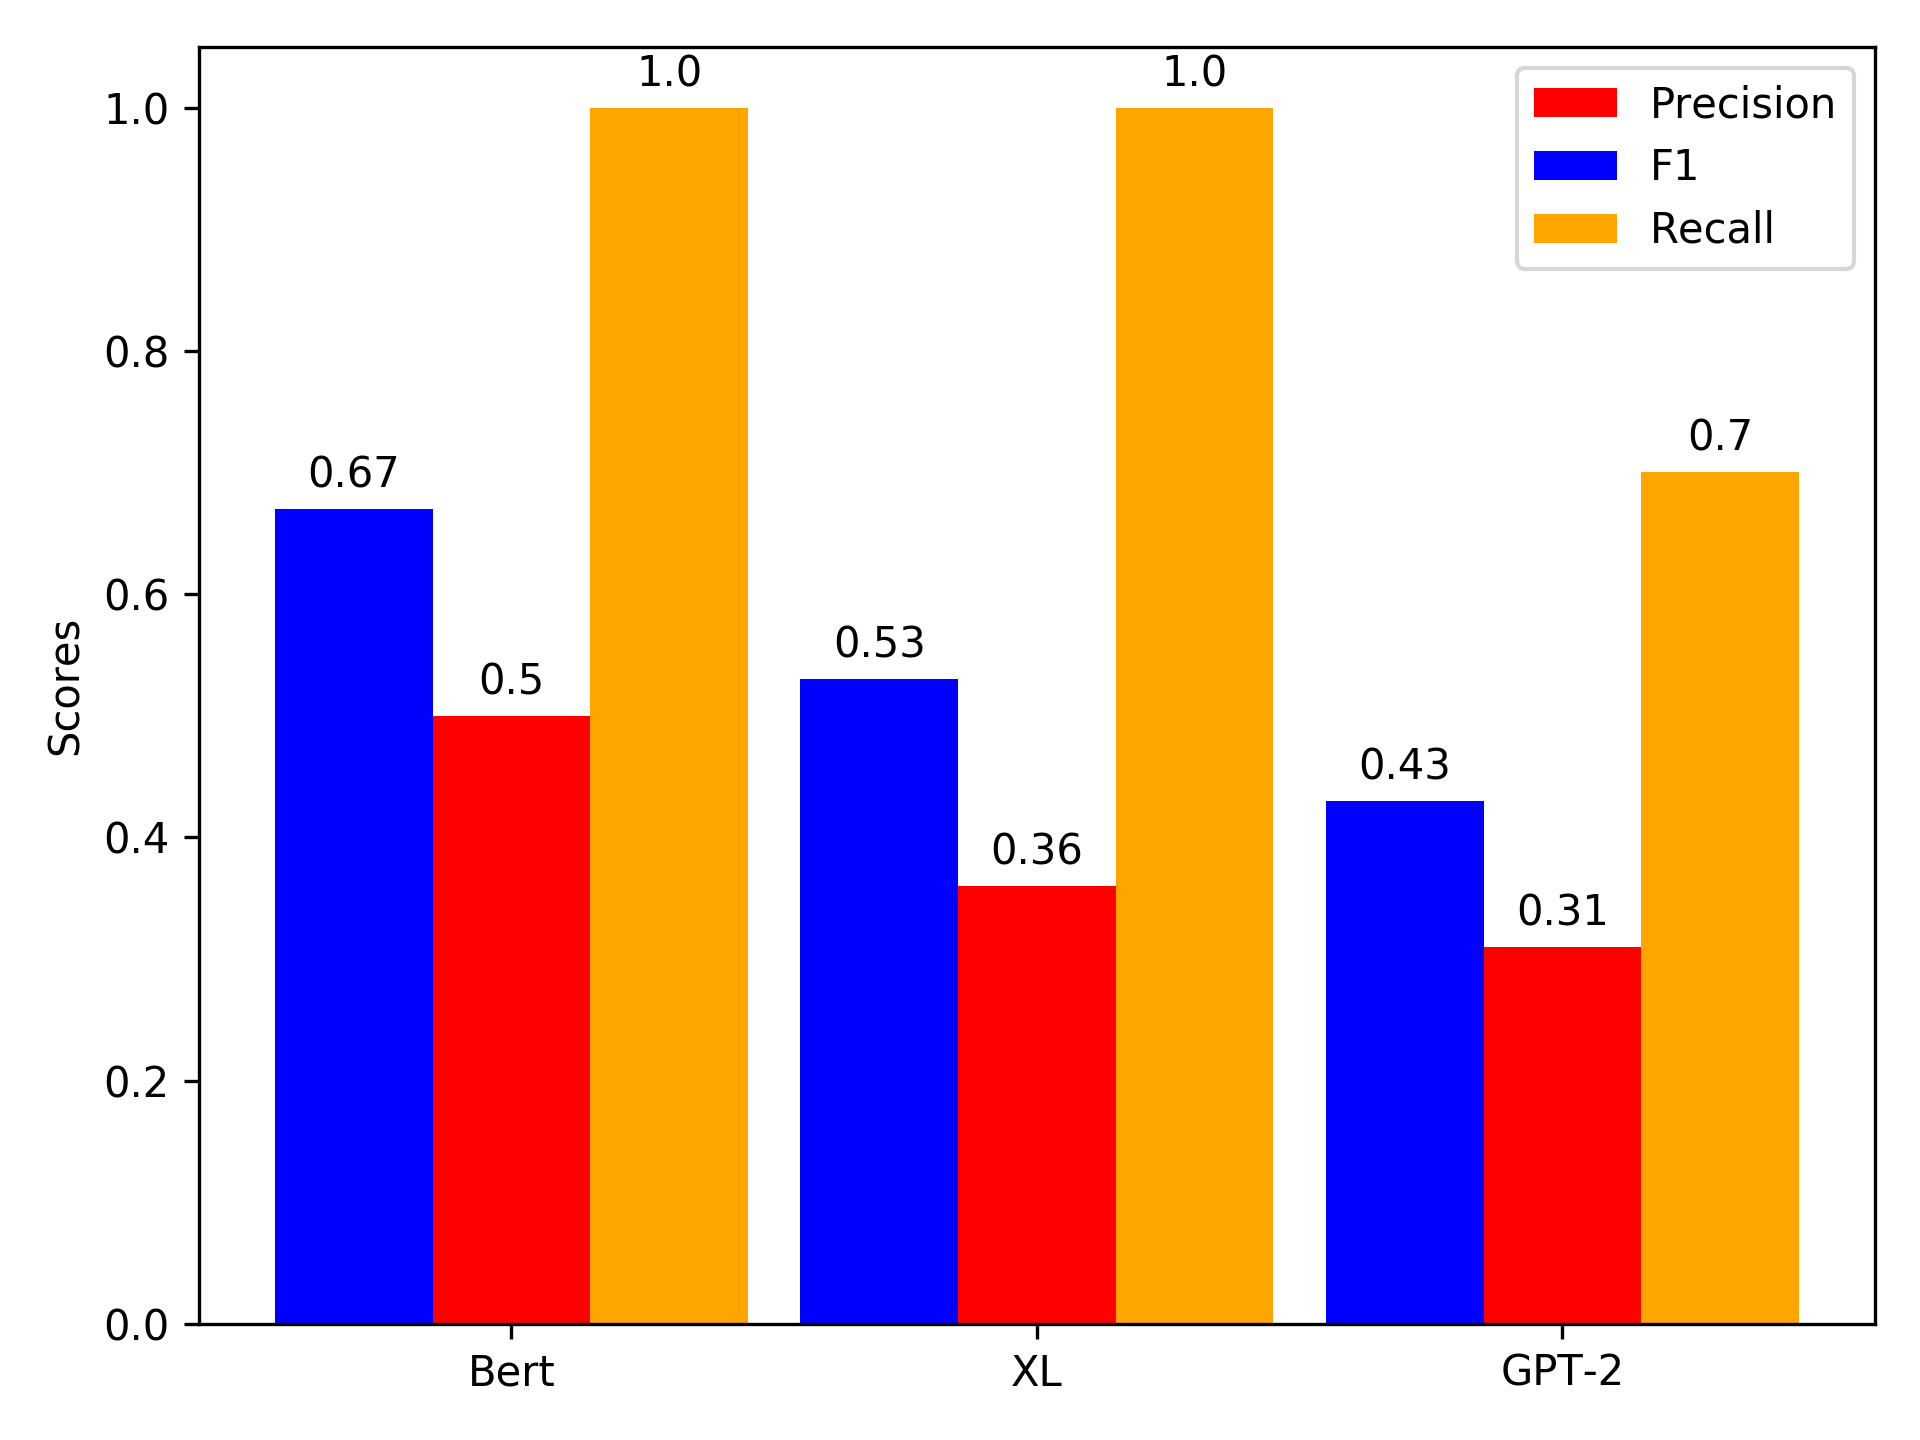
\includegraphics[trim={1cm 0.5cm 0cm 1cm}, width=0.322\textwidth]{results/average/multiclass_qualitative_average_ratio_0.15.png}}\\
\caption{\label{fig:results_multiclass_qualitative}Altering log events at different ratios, using classification.}
\end{figure*}

% multiclass sequence length
\begin{figure}[h]
  \centering
  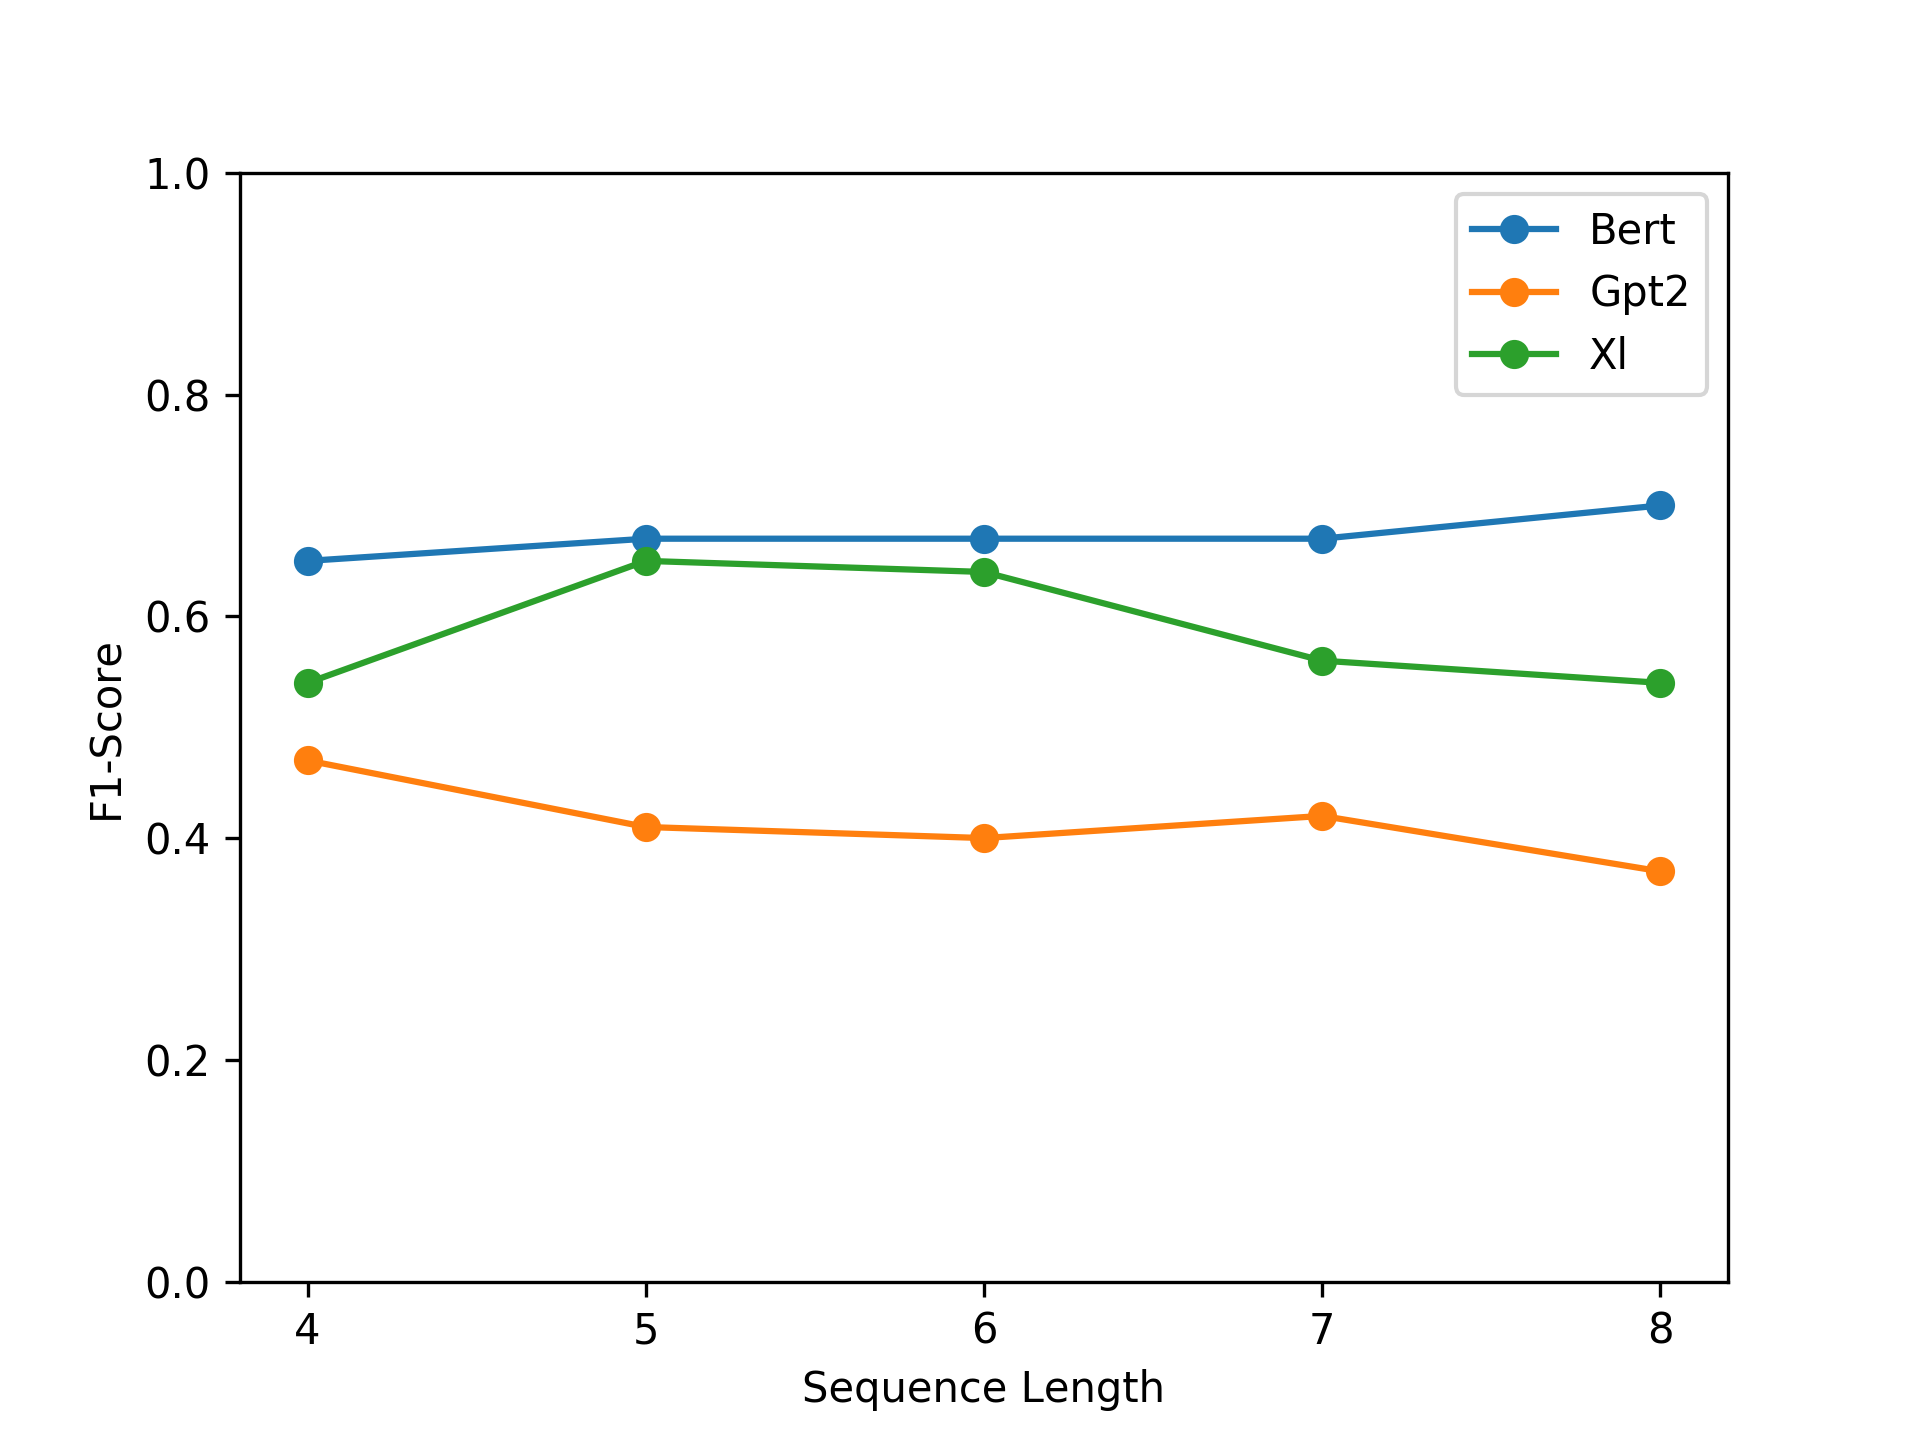
\includegraphics[width=9cm,height=6.5cm]{results/seq_len/sequence_len_classification.png}\\
  \caption{F1-Score for different input sequence lengths, with 15\% word insertion, using classification.}
  \label{fig:seq_len_classification}
\end{figure}


%%%%%
%%%%%
%%%%%

%%%%%%% TRANSFER LEARNING
%\subsection{Transfer Learning\label{sec:results_transfer}}
%In this subsection, the results of the transfer learning experiment are presented, using the classification-based approach in \ref{sec:results-classification-transfer} and the regression-based approach in \ref{sec:results-regression-transfer}.


\subsection{Transfer learning using the regression-based approach \label{sec:results-regression-transfer}}

As described in \ref{sec:transfer_learning_setup}, the alterations that were injected separately in the experiments on one dataset in the last section, are now injected all at once, in order to simulate a different dataset B. Figure \ref{fig:results_transfer_regression} shows the results for alterations on 5\%, 10\% and 15\% of the log lines of all possible alterations at the same time, after 60 epochs of training on the train dataset A and 5 epochs of training on the train dataset B. It is clearly visible, that Bert and XL-Transformers are both degrading substantially in all metrics, yet GPT-2 achieves good results even with an increased alteration ratio.

\begin{comment}
\begin{figure}[h]
  \centering
  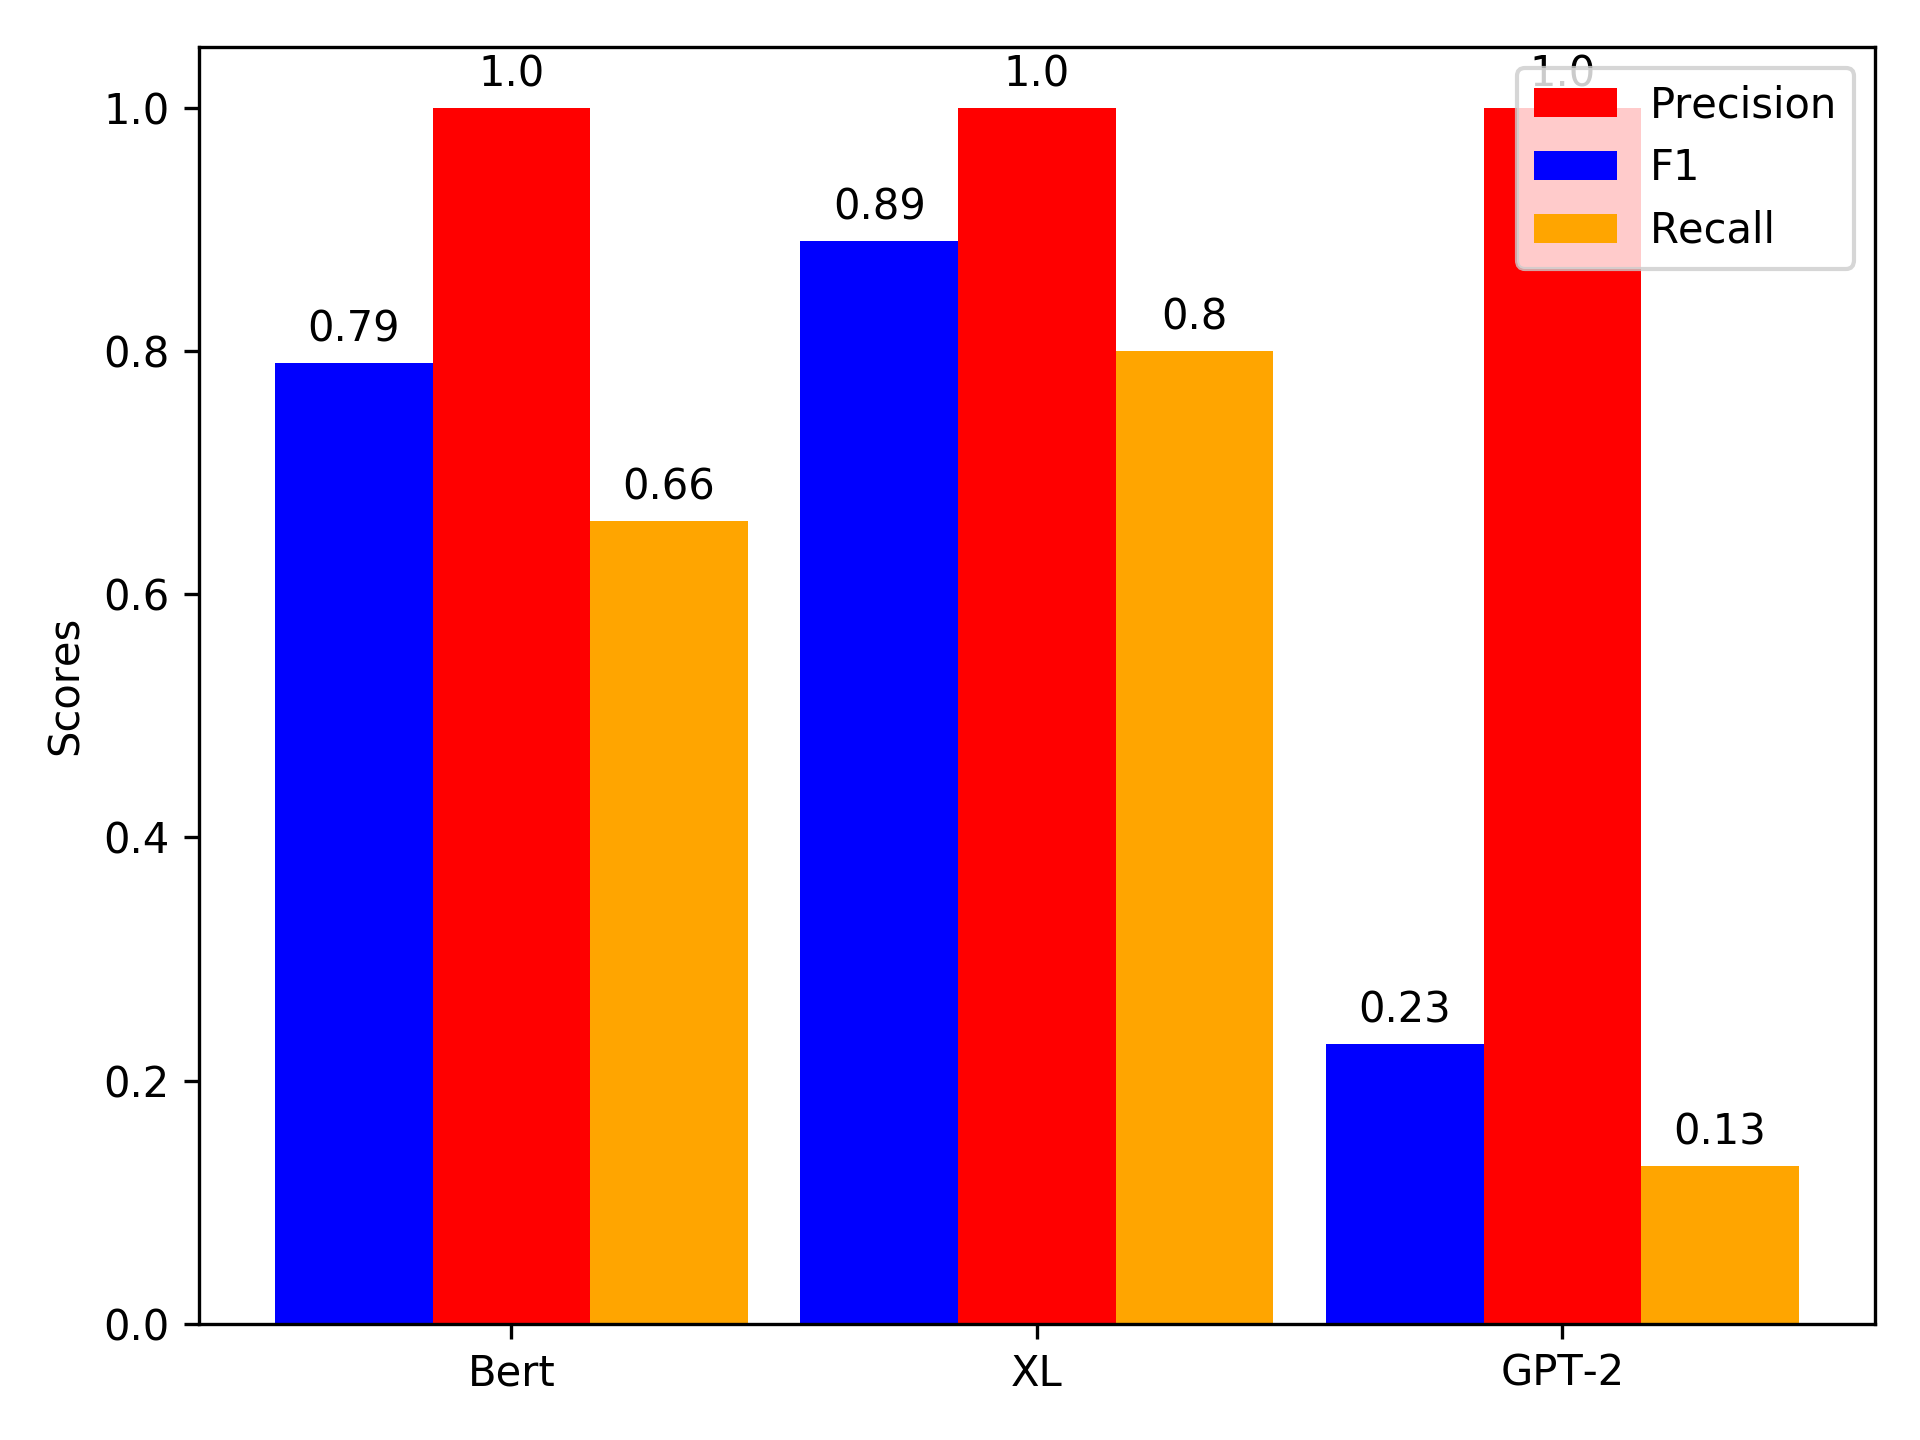
\includegraphics[width=6cm,height=4.5cm]{results/transfer/transfer_regression_reverse.png}\\
  \caption{Scores for detecting reversed order of log events for transfer learning, using regression.}
  \label{fig:regression_transfer_reverse}
\end{figure}
\end{comment}

\begin{figure*}[ht!]
  \centering
  \captionsetup{justification=centering}
   \subfloat[5\% alteration\label{fig:results_transfer_regression_0.05}]{%
      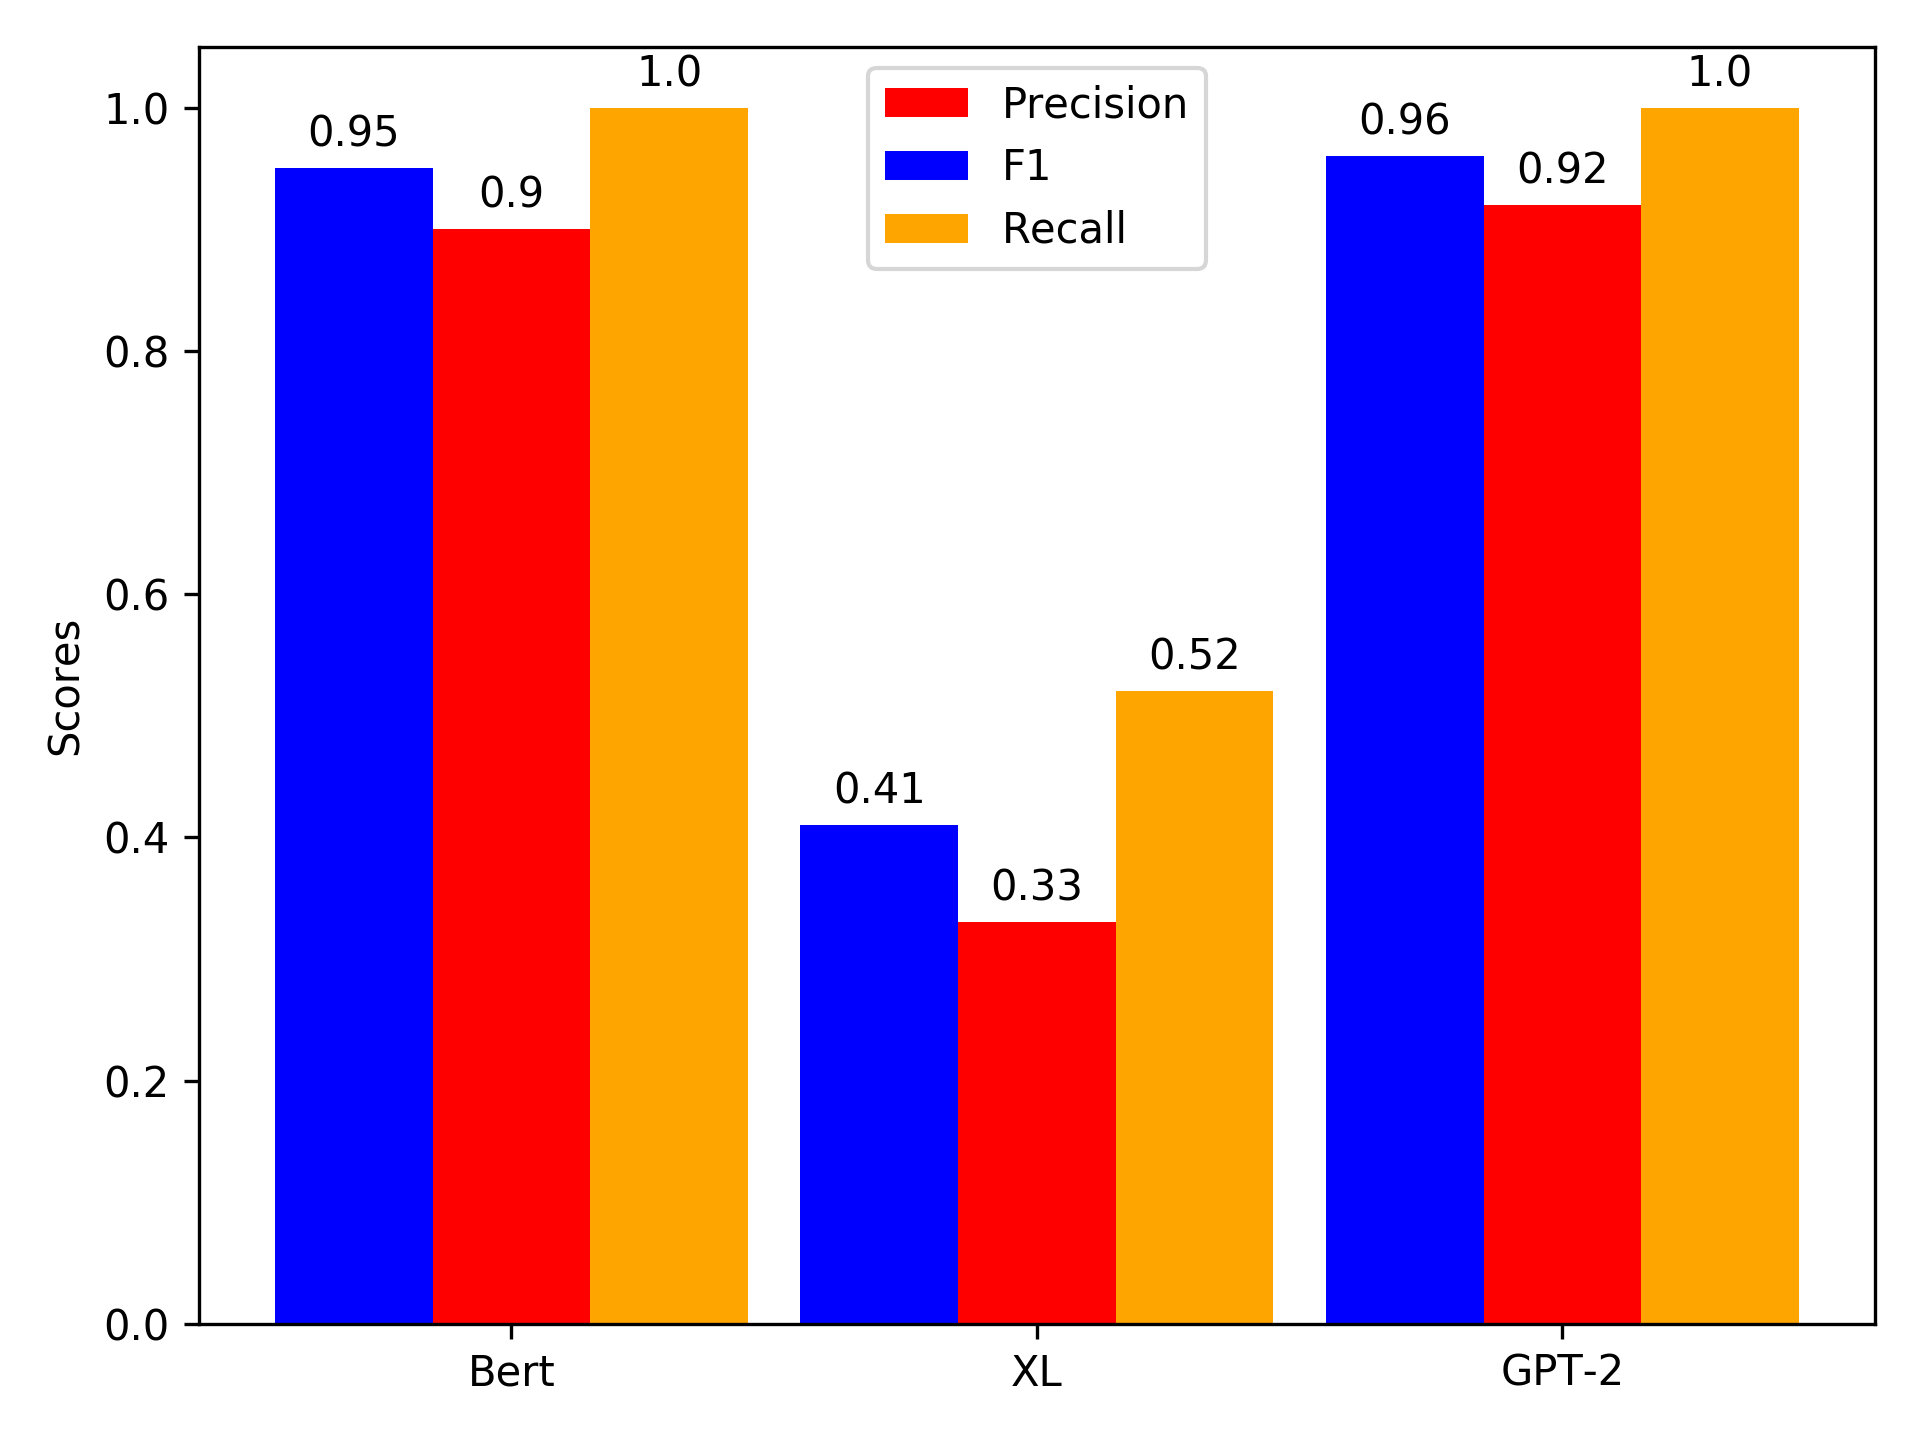
\includegraphics[trim={1cm 0.5cm 0cm 1cm}, width=0.322\textwidth]{results/transfer/transfer_regression_0.05_ratio.png}}
\hspace{\fill}
   \subfloat[10\% alteration\label{fig:results_transfer_regression_0.10} ]{%
      \includegraphics[trim={1cm 0.5cm 0cm 1cm}, width=0.322\textwidth]{results/transfer/transfer_regression_0.1_ratio.png}}
\hspace{\fill}
   \subfloat[15\% alteration\label{fig:results_transfer_regression_0.15}]{%
      \includegraphics[trim={1cm 0.5cm 0cm 1cm}, width=0.322\textwidth]{results/transfer/transfer_regression_0.15_ratio.png}}\\
\caption{\label{fig:results_transfer_regression}Transfer learning with different ratios of alteration, using regression.}
\end{figure*}


Figure \ref{fig:results_transfer_regression_per_epoch} depicts the development of the metrics of detecting anomalies for every additional epoch of training on dataset B. It is clearly visible, that XL-Transformers improves the most per epoch, although starting from a relatively low starting point, whereas Bert has a smaller increase per training epoch. The results of GPT-2 do not change much per epoch, but start at a very high level already, corresponding to the findings already made on GPT-2 using regression in \ref{sec:results-regression}. These findings are confirmed by the ROC curve plots which can be seen in figure \ref{fig:results_transfer_regression_roc}, showing nearly perfect results for GPT-2, very good results for Bert and far less satisfying results for XL-Transformers.

\begin{figure*}[ht!]
   \subfloat[Bert\label{fig:results_transfer_regression_per_epoch_0.05}]{%
      \includegraphics[trim={1cm 0.5cm 0cm 1cm}, width=0.322\textwidth]{results/transfer/bert_regression_0.15_transfer_metrics_per_epoch.png}}
\hspace{\fill}
   \subfloat[GPT-2\label{fig:results_transfer_regression_per_epoch_0.10} ]{%
      \includegraphics[trim={1cm 0.5cm 0cm 1cm}, width=0.322\textwidth]{results/transfer/gpt_regression_0.15_transfer_metrics_per_epoch.png}}
\hspace{\fill}
   \subfloat[XL\label{fig:results_transfer_regression_per_epoch_0.15}]{%
      \includegraphics[trim={1cm 0.5cm 0cm 1cm}, width=0.322\textwidth]{results/transfer/xl_regression_0.15_transfer_metrics_per_epoch.png}}\\
\caption{\label{fig:results_transfer_regression_per_epoch}Improvement of metrics per additional learning epoch, using regression.}
\end{figure*}


\begin{figure*}[ht!]
   \subfloat[Bert\label{fig:roc_curve_bert_transfer_regression}]{%
      \includegraphics[trim={1cm 0.5cm 0cm 1cm}, width=0.322\textwidth]{results/transfer/roc_curve_transfer_regression_bert_0.15.png}}
\hspace{\fill}
   \subfloat[GPT-2\label{fig:roc_curve_gpt_transfer_regression} ]{%
      \includegraphics[trim={1cm 0.5cm 0cm 1cm}, width=0.322\textwidth]{results/transfer/roc_curve_transfer_regression_gpt_0.15.png}}
\hspace{\fill}
   \subfloat[XL\label{fig:roc_curve_xl_transfer_regression}]{%
      \includegraphics[trim={1cm 0.5cm 0cm 1cm}, width=0.322\textwidth]{results/transfer/roc_curve_transfer_regression_xl_0.15.png}}\\
\caption{\label{fig:results_transfer_regression_roc}ROC-Curve for transfer learning using regression with 15\% alterations.}
\end{figure*}



%%%% TRANSFER LEARNING CLASSIFICATION
\subsection{Transfer learning using the classification-based approach \label{sec:results-classification-transfer}}

For transfer learning using the classification-based approach, the same experiments as described in \ref{sec:results-regression-transfer} were conducted. Figure \ref{fig:results_transfer_classification} shows the results of the transfer learning experiment. Interesting observations include the stable results achieved using Bert, which are little sensitive to increasing alteration ratios. Bert achieves a F-1 score of 0.82 for 5\% alterations, 0.77 for 10\% alterations and 0.81 for 15\% alterations, proving that Bert has clear advantages over GPT-2 and XL-Transformers for the classification-based approach and the results of GPT-2, which are not as good as compared to the regression-based approach. It is noticeable, that all language models achieve a recall value of 1.0.
Figure \ref{fig:results_transfer_multiclass_per_epoch} depicts the development of the metrics of detecting anomalies for every additional epoch of training on dataset B. After every epoch of training on the train dataset B, the labelled test dataset B is fed into the model, and metrics are collected. Bert improves the most per epoch, ramping up steeply in accuracy and especially for F-1 score and precision between epoch four and five. GPT-2 shows almost no improvements, with F1, precision and accuracy and XL-Transformers has small improvements over the course of the 5 epochs. These findings are confirmed by the ROC curve plots which can be seen in figure \ref{fig:results_transfer_multiclass_roc}, showing very good results for Bert, acceptable results for Xl-Transformers and far less satisfying results for GPT-2.

%\begin{figure}[h]
%  \centering
%  \includegraphics[width=6cm,height=4.5cm]{results/transfer/transfer_classification_reverse.png}\\
%  \caption{Scores for detecting reversed order of log events for transfer learning, using classification.}
%  \label{fig:classification_transfer_reverse}
  
%\end{figure}
\begin{figure*}[ht!]
   \subfloat[5\% alteration\label{fig:results_transfer_classification_0.05}]{%
      \includegraphics[trim={1cm 0.5cm 0cm 1cm}, width=0.322\textwidth]{results/transfer/transfer_multiclass_0.05_ratio.png}}
\hspace{\fill}
   \subfloat[10\% alteration\label{fig:results_transfer_classification_0.10} ]{%
      \includegraphics[trim={1cm 0.5cm 0cm 1cm}, width=0.322\textwidth]{results/transfer/transfer_multiclass_0.1_ratio.png}}
\hspace{\fill}
   \subfloat[15\% alteration\label{fig:results_transfer_classification_0.15}]{%
      \includegraphics[trim={1cm 0.5cm 0cm 1cm}, width=0.322\textwidth]{results/transfer/transfer_multiclass_0.15_ratio.png}}\\
\caption{\label{fig:results_transfer_classification}Transfer learning with different ratios of alteration, using classification.}
\end{figure*}

\begin{figure*}[ht!]
   \subfloat[Bert\label{fig:results_transfer_multiclass_per_epoch_0.05}]{%
      \includegraphics[trim={1cm 0.5cm 0cm 1cm}, width=0.322\textwidth]{results/transfer/bert_multiclass_0.15_transfer_metrics_per_epoch.png}}
\hspace{\fill}
   \subfloat[GPT-2\label{fig:results_transfer_multiclass_per_epoch_0.10} ]{%
      \includegraphics[trim={1cm 0.5cm 0cm 1cm}, width=0.322\textwidth]{results/transfer/gpt_multiclass_0.15_transfer_metrics_per_epoch.png}}
\hspace{\fill}
   \subfloat[XL\label{fig:results_transfer_multiclass_per_epoch_0.15}]{%
      \includegraphics[trim={1cm 0.5cm 0cm 1cm}, width=0.322\textwidth]{results/transfer/xl_multiclass_0.15_transfer_metrics_per_epoch.png}}\\
\caption{\label{fig:results_transfer_multiclass_per_epoch}Improvement of metrics per additional learning epoch, using classification.}
\end{figure*}


\begin{figure*}[ht!]
   \subfloat[Bert\label{fig:roc_curve_bert_transfer_multiclass}]{%
      \includegraphics[trim={1cm 0.5cm 0cm 1cm}, width=0.322\textwidth]{results/transfer/roc_curve_transfer_multiclass_bert_0.15.png}}
\hspace{\fill}
   \subfloat[GPT-2\label{fig:roc_curve_gpt_transfer_multiclass} ]{%
      \includegraphics[trim={1cm 0.5cm 0cm 1cm}, width=0.322\textwidth]{results/transfer/roc_curve_transfer_multiclass_gpt_0.15.png}}
\hspace{\fill}
   \subfloat[XL\label{fig:roc_curve_xl_transfer_multiclass}]{%
      \includegraphics[trim={1cm 0.5cm 0cm 1cm}, width=0.322\textwidth]{results/transfer/roc_curve_transfer_multiclass_xl_0.15.png}}\\
\caption{\label{fig:results_transfer_multiclass_roc}ROC-Curve for transfer learning using regression with 15\% alterations.}
\end{figure*}



\section{Discussion of Results\label{sec:discussion_results}}
By evaluating three different language models, it has been shown that the used word embeddings can highly influence the quality of the results for anomaly detection, with different word embeddings having strengths and weaknesses in different categories. 

\begin{comment}
For anomaly detection on one dataset using the regression approach, GPT-2 shows strong results, with F1-Scores of 0.95 when altering 5\% of log sequences, and 0.93 when altering the log lines, the quality of the results don't degrade much, when alteration ratios are increased, where Bert and XL-Transformers show decreases of 0.1 to 0.2 percentage points when increasing the alteration ratio from 5\% to 15\%. Yet, when the log events are completely reversed, GPT-2 achieves an F1-Score of only 0.55, where Bert and XL achieve 0.98, almost perfectly detecting the wrong sequence of log events.
\end{comment}

For the regression approach on one dataset, GPT-2 beats Bert and XL-Transformers clearly with regards to all metrics.

For the classification approach on one dataset on the other hand, GPT-2 shows weaker results than XL-Transformers and Bert. This is probably party due to the small cosine distance between the embeddings of the templates, where small changes on the templates can have a high impact already.

For the transfer learning approach, the results show a slightly different picture. Using the regression approach, GPT-2 is still ahead of the other two, while Bert seems to show better results than for detection on one dataset. 

On the other hand, for transfer learning using the classification-based approach, for 15\% alteration, GPT-2 shows results that are not much better than random, while still being able to find all anomalies, but showing a small F1-Score of only 0.17, where Bert is able to reach a F1-Score of 0.81. It is also visible, that GPT-2 seems to not profit as much from the few-show learning on dataset B, where the metrics stay almost the same throughout, yet Bert shows improvements from an F1-Score of 0.3 to 0.8.

It is evident, that with more hyperparameter-tuning, far better results can be accomplished, especially with XL-Transformers, since it obviously requires a different setup of hidden units and layers within the LSTM to achieve optimal results, however, since the model is a prototype and is supposed to show the possibility of comparing different word embeddings, not all potentials were fully tapped.

%TODO box plots of loss values in 
    \chapter{Related Work\label{cha:related_work}}


\section{Sequence-Based Anomaly Detection in Logs}

\subsection{DeepLog: Anomaly Detection and Diagnosis from System Logs through Deep Learning}
Du et al. proposed DeepLog \cite{du2017deeplog}, a prominent example of a model that treats system logs as natural language sequences. An overview of the model is depicted in figure \ref{fig:deeplog}. The first step of the proposed model is like in most of the works in the area: Logs are first pre-processed with a log parser, they separate the constant from the variable part. Log templates are mapped to log keys $k_i$, which are just indices between $0$ to the number of different templates. For each log entry $e_i$, the elapsed time between $e_i$ and $e_{i-1}$ are stored in $\vec{v}_{e_i}$, together with parameter values in a parameter value vector. An LSTM is then trained on the sequences $k_i$ to learn normal system execution paths. Given a window size of $h=3$, a sequence of log keys $\{k_5, k_{11}, k_2, k_{14}, k_{15}\}$ would results in the \textit{input sequence} and \textit{output sequence} for training of $\{k_{5},k_{11},k_{2} \rightarrow k_{14}\}$ and $\{k_{11},k_{2},k_{14} \rightarrow k_{15}\}$. Given these sequences of keys, the system is trained to maximise the probability of having $k_i \in K$ as the next log key value, thus learning the probability distribution $Pr(m_t = k_i | m_{t-h},...,m_{t-1})$, so given a log key sequence of length $h$, outputs a probability distribution of all possible log key values. A log key value is treated as normal, if it's among the top $g$ candidates.
 For the detection stage, new log key entries $e_t$ are parsed into a log key $m_t$ and parameter value vector. Then, the trained model is used, to check if the incoming log key is normal, by sending $w = \{m_{t-h}, ..., m_{t-1}\}$ as input. Additionally, the parameter value vector is checked. If the log entry is labeled being abnormal, the model provides semantic information for users to manually diagnose the anomaly. In order to adapt to changing patterns and log entries, the user has the possibility to mark a detected anomaly as a false positive, thus updating the model.

For verification of the model, the authors deployed an OpenStack experiment to fabricate their own log data. They produce over 1 million log entries, with 7\% being abnormal. The model is able to achieve a precision of 0.96, recall of 1.0 and F1-score of 0.98.

Even though the model can be adjusted after the training phase on a particular dataset is already completed, by manually reporting false positives, thus enabling the system to adapt to changing or new sequences of logs, it is not able to dynamically adapt to changes on the log events themselves. If log data changes on the log event level, re-training of the model is necessary.

\begin{figure}[h]
  \centering
  \includegraphics[width=15cm]{deeplog.png}\\
  \caption{DeepLog model overview \cite{graves2013speech}}
  \label{fig:deeplog}
\end{figure}


\subsection{LogAnomaly: Unsupervised Detection of Sequential and Quantitative Anomalies in Unstructured Logs}
LogAnomaly, the approach proposed by Meng et al. \cite{meng2019loganomaly} models a log stream as a natural language sequence. Log event sequences are first parsed into template sequences. These sequences are then transformed into embedding sequences using a novel word representation method, template2Vec.

\begin{figure}[h]
  \centering
  \includegraphics[width=15cm]{LogAnomaly.png}\\
  \caption{DeepLog model overview \cite{graves2013speech}}
  \label{fig:deeplog}
\end{figure}

There has been a large amount of research and development of new approaches for anomaly detection in logs. %TODO alle Quellen einfuegen.
Approaches can be characterised by the following categories: supervised learning models, unsupervised learning models, statistical models, classical machine learning models and finally deep learning models.
% supervised learning methods
Numerous supervised learning methods were applied to solve the problem of log anomaly detection. Liang et al. \cite{liang2007failure} and Yuan et al. \cite{yuan2006automated} trained a SVM classifier to detect errors. Farshchi et al. \cite{farshchi2015anomaly} adopt a regression-based method to find correlations between an operation's logs and the operation activity's effect on cloud resources. Chen et al \cite{chen2004failure} presented a decision tree learning approach to diagnose failures in large Internet sites. However, these methods have two limitations: they rely on system-specific labeled log data for training and do not provide a general method to cope with ever-changing log data.
% unsupervised learning methods

Additionally, unsupervised learning methods have been proposed. Xu et al. \cite{xu2009detecting} use the Principal Component Analysis method to construct a log count matrix, grouping log events to sessions with the session id which is available for every log event. Lin et al \cite{lin2016log} and \cite{vaarandi2003data} both propose approaches that cluster logs.

% deep learning
The recent remarkable advances of deep learning depict new promising paths for anomaly detection in logs. While LSTMs have been put to use in detecting anomalies in time series generally \cite{malhotra2015long}, they have been used in anomaly detection in logs: Du et al. \cite{du2017deeplog} present DeepLog: first, log events are mapped to keys, the sequential order of these keys is learned using a LSTM to detect anomalies. Zhang et al. \cite{zhang2016automated} use a LSTM similarly. Even though these approaches yield good results, they are not able to cope with changing log data, since log events have to be transformed into fixed indices.

% nlp based
There are studies that have applied NLP techniques and consider log events as natural language. Bertero et al \cite{bertero2017experience} used Google's word2vec algorithm to obtain word embeddings, exploiting the obtained feature space using standard classifiers, like SVM and Random Forest, to detect anomalies. Zhang et al. \cite{zhang2016automated} additionally to using the LSTM model for time series prediction, apply  TF-IDF weight and consider each log event as a word. Brown et al. \cite{brown2018recurrent} use combine attention based models together with word word embeddings. These approaches do not take into account the contextual information in log sequences.

Recently, LogRobust and LogAnomaly use pre-trained word embeddings, using an attention-based Bi-LSTM model to learn log sequences.
    \chapter{Conclusion\label{cha:conclusion}}



\section{Summary\label{sec:summary}}

Finding suitable representations for log data in the form of word embeddings is an important step towards building a robust, environment-agnostic anomaly detection model. This work presents an evaluation of three different word embedding models, namely Bert, GPT-2 and XL-Transformers and compares them using a regression-based and a classification-based approach. Additionally, in order to evaluate the robustness of the model, different alterations are injected into the logs. These alterations are finally combined together, to simulate the existence of a different log dataset B and the portability of obtained knowledge from training on a log dataset A.

The work done can be summarised by the following steps:
\begin{itemize}
		\item Finding a suitable log parser by evaluating the available log parsers on their performance on the log dataset.
		\item Finding suitable language models in order to represent log templates so that they can be used for the task of anomaly detection
		\item Finding a means to alter log datasets in such a way that the existence of a different log dataset and the evolution of log data can be simulated in oder to evaluate the performance of the transfer learning method.
		\item Evaluation of the proposed model by comparing the quality of word embeddings obtained by different pre-trained language models with regards to the task of anomaly detection in system logs.
\end{itemize}


\section{Problems Encountered\label{sec:problems}}
Several impediments occurred during the development of the model. 

At the beginning, it was not obvious, which word embeddings to use in order to represent log events. First attempts were made with GloVe, using word vectors that were trained only the available small log corpus, since the publicly available pre-trained vectors did not have representations for log-domain-specific words like "MB", "GB", "deallocate", "VM". These representations of log events of unequal length were padded with zeros and fed into an Auto Encoder, in order to learn the sentence representations. Then, the latent space representation of every log event was used in order to obtain representations of equal length. This attempt yielded acceptable results on the easiest case of injecting anomalies without alterations, but were disappointing when injecting alterations, making it unfit for the transfer approach. This was unfortunate, since a lot of time was invested into this approach. Using more sophisticated language models like Bert delivered better results overall.

Finding appropriate hyperparameters for the model, for example sequence length, number of hidden units and number of layers for the LSTM or clipping, was not easy in the beginning, since all of them heavily influence the end result if not set correctly. A lot of development time was invested, trying to find the reasons for problems elsewhere, when the only problem was for example a wrongly chosen value for gradient clipping.

\section{Outlook\label{sec:outlook}}
A very important step in order to make the proposed model even more robust, resilient and most importantly able to transfer knowledge on new datasets, evaluation into finding a proper attention mechanism that fits the use-case correctly and enhances it. The mentioned papers in \ref{cha:related_work} have proven that using an attention mechanism in combination with a LSTM can highly improve the results obtained from the model.

Fine-tuning a pre-trained language model explicitly on the task of anomaly detection by integrating the fine-tuning step into the model's pipeline, can potentially improve the quality of the word embeddings. This can especially be useful for the transfer learning task.





% ---------------------------------------------------------------
\backmatter % no page numbering from here
    \addchap{List of Acronyms}

\begin{tabbing}
spacespacespace \= space \kill
3GPP	 \> 	3rd Generation Partnership Project	 \\
AJAX	\>	Asynchronous JavaScript and XML \\
\end{tabbing}
\endinput

		
		% if you want to provide a glossary with explanations of important terms put it in here

    \bibliographystyle{ieeetr}
    \bibliography{./bib/references}
    
    \addchap{Annex}

\begin{appendix}

\begin{comment}
%
%%%%%%%%%%%%%%%%%%%%%%%%%%%%%%%%%%%%%%%%%%%%%%%%%%%%%%%%%%%%%%%%%%%%%%%%
%%%%%%%%%%%%%%%%%%%%%%%%%%%%%%%%%%%%%%%%%%%%%%%%%%%%%%%%%%%%%%%%%%%%%%%%
%			R E G R E S S I O N
%%%%%%%%%%%%%%%%%%%%%%%%%%%%%%%%%%%%%%%%%%%%%%%%%%%%%%%%%%%%%%%%%%%%%%%%
%%%%%%%%%%%%%%%%%%%%%%%%%%%%%%%%%%%%%%%%%%%%%%%%%%%%%%%%%%%%%%%%%%%%%%%%
\section{Regression}
%%%%%%%%%%%%%%%%%%%%%%%%%%%%%%%%%%%%
%			INSERT WORDS
%%%%%%%%%%%%%%%%%%%%%%%%%%%%%%%%%%%%
\begin{table}
\centering
\begin{tabular}{ c l l l l }
\toprule
Injection Ratio & Metric & Bert & XL & GPT-2\\
\midrule
     & F1-Score & 0.2232 & 0.6223 & 0.892\\
5\%  & Precision & 0.2416 & 0.4449 & 0.892\\
     & Recall & 0.0024 & 0.0047 & 0.892\\ 
\midrule
     & F1-Score & 0.2232 & 0.6223 & 0.892\\
10\% & Precision & 0.2416 & 0.4449 & 0.892\\
     & Recall & 0.0024 & 0.0047 & 0.892\\ 
\midrule
     & F1-Score & 0.2232 & 0.6223 & 0.892\\
15\% & Precision & 0.2416 & 0.4449 & 0.892\\
     & Recall & 0.0024 & 0.0047 & 0.892\\ 
\bottomrule
\end{tabular}
\caption{Experiment results on inserting one word.}
\end{table}



%%%%%%%%%%%%%%%%%%%%%%%%%%%%%%%%%%%%
%			REMOVE WORDS
%%%%%%%%%%%%%%%%%%%%%%%%%%%%%%%%%%%%
\begin{table}
\centering
\begin{tabular}{ c l l l l }
\toprule
Injection Ratio & Metric & Bert & XL & GPT-2\\
\midrule
     & F1-Score & 0.2232 & 0.6223 & 0.892\\
5\%  & Precision & 0.2416 & 0.4449 & 0.892\\
     & Recall & 0.0024 & 0.0047 & 0.892\\ 
\midrule
     & F1-Score & 0.2232 & 0.6223 & 0.892\\
10\% & Precision & 0.2416 & 0.4449 & 0.892\\
     & Recall & 0.0024 & 0.0047 & 0.892\\ 
\midrule
     & F1-Score & 0.2232 & 0.6223 & 0.892\\
15\% & Precision & 0.2416 & 0.4449 & 0.892\\
     & Recall & 0.0024 & 0.0047 & 0.892\\ 
\bottomrule
\end{tabular}
\caption{Experiment results on removing one word.}
\end{table}


%%%%%%%%%%%%%%%%%%%%%%%%%%%%%%%%%%%%
%			REPLACE WORDS
%%%%%%%%%%%%%%%%%%%%%%%%%%%%%%%%%%%%
\begin{table}
\centering
\begin{tabular}{ c l l l l }
\toprule
Injection Ratio & Metric & Bert & XL & GPT-2\\
\midrule
     & F1-Score & 0.2232 & 0.6223 & 0.892\\
5\%  & Precision & 0.2416 & 0.4449 & 0.892\\
     & Recall & 0.0024 & 0.0047 & 0.892\\ 
\midrule
     & F1-Score & 0.2232 & 0.6223 & 0.892\\
10\% & Precision & 0.2416 & 0.4449 & 0.892\\
     & Recall & 0.0024 & 0.0047 & 0.892\\ 
\midrule
     & F1-Score & 0.2232 & 0.6223 & 0.892\\
15\% & Precision & 0.2416 & 0.4449 & 0.892\\
     & Recall & 0.0024 & 0.0047 & 0.892\\ 
\bottomrule
\end{tabular}
\caption{Experiment results on replacing one word.}
\end{table}



%%%%%%%%%%%%%%%%%%%%%%%%%%%%%%%%%%%%
%			SHUFFLE LINES
%%%%%%%%%%%%%%%%%%%%%%%%%%%%%%%%%%%%
\begin{table}
\centering
\begin{tabular}{ c l l l l }
\toprule
Injection Ratio & Metric & Bert & XL & GPT-2\\
\midrule
     & F1-Score & 0.2232 & 0.6223 & 0.892\\
5\%  & Precision & 0.2416 & 0.4449 & 0.892\\
     & Recall & 0.0024 & 0.0047 & 0.892\\ 
\midrule
     & F1-Score & 0.2232 & 0.6223 & 0.892\\
10\% & Precision & 0.2416 & 0.4449 & 0.892\\
     & Recall & 0.0024 & 0.0047 & 0.892\\ 
\midrule
     & F1-Score & 0.2232 & 0.6223 & 0.892\\
15\% & Precision & 0.2416 & 0.4449 & 0.892\\
     & Recall & 0.0024 & 0.0047 & 0.892\\ 
\bottomrule
\end{tabular}
\caption{Experiment results on shuffling lines.}
\end{table}



%%%%%%%%%%%%%%%%%%%%%%%%%%%%%%%%%%%%
%			DUPLICATE LINES
%%%%%%%%%%%%%%%%%%%%%%%%%%%%%%%%%%%%
\begin{table}
\centering
\begin{tabular}{ c l l l l }
\toprule
Injection Ratio & Metric & Bert & XL & GPT-2\\
\midrule
     & F1-Score & 0.2232 & 0.6223 & 0.892\\
5\%  & Precision & 0.2416 & 0.4449 & 0.892\\
     & Recall & 0.0024 & 0.0047 & 0.892\\ 
\midrule
     & F1-Score & 0.2232 & 0.6223 & 0.892\\
10\% & Precision & 0.2416 & 0.4449 & 0.892\\
     & Recall & 0.0024 & 0.0047 & 0.892\\ 
\midrule
     & F1-Score & 0.2232 & 0.6223 & 0.892\\
15\% & Precision & 0.2416 & 0.4449 & 0.892\\
     & Recall & 0.0024 & 0.0047 & 0.892\\ 
\bottomrule
\end{tabular}
\caption{Experiment results on duplicating lines.}
\end{table}


%%%%%%%%%%%%%%%%%%%%%%%%%%%%%%%%%%%%
%			DELETE LINES
%%%%%%%%%%%%%%%%%%%%%%%%%%%%%%%%%%%%
\begin{table}
\centering
\begin{tabular}{ c l l l l }
\toprule
Injection Ratio & Metric & Bert & XL & GPT-2\\
\midrule
     & F1-Score & 0.2232 & 0.6223 & 0.892\\
5\%  & Precision & 0.2416 & 0.4449 & 0.892\\
     & Recall & 0.0024 & 0.0047 & 0.892\\ 
\midrule
     & F1-Score & 0.2232 & 0.6223 & 0.892\\
10\% & Precision & 0.2416 & 0.4449 & 0.892\\
     & Recall & 0.0024 & 0.0047 & 0.892\\ 
\midrule
     & F1-Score & 0.2232 & 0.6223 & 0.892\\
15\% & Precision & 0.2416 & 0.4449 & 0.892\\
     & Recall & 0.0024 & 0.0047 & 0.892\\ 
\bottomrule
\end{tabular}
\caption{Experiment results on deleting lines.}
\end{table}



%%%%%%%%%%%%%%%%%%%%%%%%%%%%%%%%%%%%%%%%%%%%%%%%%%%%%%%%%%%%%%%%%%%%%%%%
%%%%%%%%%%%%%%%%%%%%%%%%%%%%%%%%%%%%%%%%%%%%%%%%%%%%%%%%%%%%%%%%%%%%%%%%
%			C L A S S I F I C A T I O N 
%%%%%%%%%%%%%%%%%%%%%%%%%%%%%%%%%%%%%%%%%%%%%%%%%%%%%%%%%%%%%%%%%%%%%%%%
%%%%%%%%%%%%%%%%%%%%%%%%%%%%%%%%%%%%%%%%%%%%%%%%%%%%%%%%%%%%%%%%%%%%%%%%

\section{Classification}

%%%%%%%%%%%%%%%%%%%%%%%%%%%%%%%%%%%%
%			INSERT WORDS
%%%%%%%%%%%%%%%%%%%%%%%%%%%%%%%%%%%%
\begin{table}
\centering
\begin{tabular}{ c l l l l }
\toprule
Injection Ratio & Metric & Bert & XL & GPT-2\\
\midrule
     & F1-Score & 0.2232 & 0.6223 & 0.892\\
5\%  & Precision & 0.2416 & 0.4449 & 0.892\\
     & Recall & 0.0024 & 0.0047 & 0.892\\ 
\midrule
     & F1-Score & 0.2232 & 0.6223 & 0.892\\
10\% & Precision & 0.2416 & 0.4449 & 0.892\\
     & Recall & 0.0024 & 0.0047 & 0.892\\ 
\midrule
     & F1-Score & 0.2232 & 0.6223 & 0.892\\
15\% & Precision & 0.2416 & 0.4449 & 0.892\\
     & Recall & 0.0024 & 0.0047 & 0.892\\ 
\bottomrule
\end{tabular}
\caption{Experiment results on inserting one word.}
\end{table}



%%%%%%%%%%%%%%%%%%%%%%%%%%%%%%%%%%%%
%			REMOVE WORDS
%%%%%%%%%%%%%%%%%%%%%%%%%%%%%%%%%%%%
\begin{table}
\centering
\begin{tabular}{ c l l l l }
\toprule
Injection Ratio & Metric & Bert & XL & GPT-2\\
\midrule
     & F1-Score & 0.2232 & 0.6223 & 0.892\\
5\%  & Precision & 0.2416 & 0.4449 & 0.892\\
     & Recall & 0.0024 & 0.0047 & 0.892\\ 
\midrule
     & F1-Score & 0.2232 & 0.6223 & 0.892\\
10\% & Precision & 0.2416 & 0.4449 & 0.892\\
     & Recall & 0.0024 & 0.0047 & 0.892\\ 
\midrule
     & F1-Score & 0.2232 & 0.6223 & 0.892\\
15\% & Precision & 0.2416 & 0.4449 & 0.892\\
     & Recall & 0.0024 & 0.0047 & 0.892\\ 
\bottomrule
\end{tabular}
\caption{Experiment results on removing one word.}
\end{table}


%%%%%%%%%%%%%%%%%%%%%%%%%%%%%%%%%%%%
%			REPLACE WORDS
%%%%%%%%%%%%%%%%%%%%%%%%%%%%%%%%%%%%
\begin{table}
\centering
\begin{tabular}{ c l l l l }
\toprule
Injection Ratio & Metric & Bert & XL & GPT-2\\
\midrule
     & F1-Score & 0.2232 & 0.6223 & 0.892\\
5\%  & Precision & 0.2416 & 0.4449 & 0.892\\
     & Recall & 0.0024 & 0.0047 & 0.892\\ 
\midrule
     & F1-Score & 0.2232 & 0.6223 & 0.892\\
10\% & Precision & 0.2416 & 0.4449 & 0.892\\
     & Recall & 0.0024 & 0.0047 & 0.892\\ 
\midrule
     & F1-Score & 0.2232 & 0.6223 & 0.892\\
15\% & Precision & 0.2416 & 0.4449 & 0.892\\
     & Recall & 0.0024 & 0.0047 & 0.892\\ 
\bottomrule
\end{tabular}
\caption{Experiment results on replacing one word.}
\end{table}



%%%%%%%%%%%%%%%%%%%%%%%%%%%%%%%%%%%%
%			SHUFFLE LINES
%%%%%%%%%%%%%%%%%%%%%%%%%%%%%%%%%%%%
\begin{table}
\centering
\begin{tabular}{ c l l l l }
\toprule
Injection Ratio & Metric & Bert & XL & GPT-2\\
\midrule
     & F1-Score & 0.2232 & 0.6223 & 0.892\\
5\%  & Precision & 0.2416 & 0.4449 & 0.892\\
     & Recall & 0.0024 & 0.0047 & 0.892\\ 
\midrule
     & F1-Score & 0.2232 & 0.6223 & 0.892\\
10\% & Precision & 0.2416 & 0.4449 & 0.892\\
     & Recall & 0.0024 & 0.0047 & 0.892\\ 
\midrule
     & F1-Score & 0.2232 & 0.6223 & 0.892\\
15\% & Precision & 0.2416 & 0.4449 & 0.892\\
     & Recall & 0.0024 & 0.0047 & 0.892\\ 
\bottomrule
\end{tabular}
\caption{Experiment results on shuffling lines.}
\end{table}



%%%%%%%%%%%%%%%%%%%%%%%%%%%%%%%%%%%%
%			DUPLICATE LINES
%%%%%%%%%%%%%%%%%%%%%%%%%%%%%%%%%%%%
\begin{table}
\centering
\begin{tabular}{ c l l l l }
\toprule
Injection Ratio & Metric & Bert & XL & GPT-2\\
\midrule
     & F1-Score & 0.2232 & 0.6223 & 0.892\\
5\%  & Precision & 0.2416 & 0.4449 & 0.892\\
     & Recall & 0.0024 & 0.0047 & 0.892\\ 
\midrule
     & F1-Score & 0.2232 & 0.6223 & 0.892\\
10\% & Precision & 0.2416 & 0.4449 & 0.892\\
     & Recall & 0.0024 & 0.0047 & 0.892\\ 
\midrule
     & F1-Score & 0.2232 & 0.6223 & 0.892\\
15\% & Precision & 0.2416 & 0.4449 & 0.892\\
     & Recall & 0.0024 & 0.0047 & 0.892\\ 
\bottomrule
\end{tabular}
\caption{Experiment results on duplicating lines.}
\end{table}


%%%%%%%%%%%%%%%%%%%%%%%%%%%%%%%%%%%%
%			DELETE LINES
%%%%%%%%%%%%%%%%%%%%%%%%%%%%%%%%%%%%
\begin{table}
\centering
\begin{tabular}{ c l l l l }
\toprule
Injection Ratio & Metric & Bert & XL & GPT-2\\
\midrule
     & F1-Score & 0.2232 & 0.6223 & 0.892\\
5\%  & Precision & 0.2416 & 0.4449 & 0.892\\
     & Recall & 0.0024 & 0.0047 & 0.892\\ 
\midrule
     & F1-Score & 0.2232 & 0.6223 & 0.892\\
10\% & Precision & 0.2416 & 0.4449 & 0.892\\
     & Recall & 0.0024 & 0.0047 & 0.892\\ 
\midrule
     & F1-Score & 0.2232 & 0.6223 & 0.892\\
15\% & Precision & 0.2416 & 0.4449 & 0.892\\
     & Recall & 0.0024 & 0.0047 & 0.892\\ 
\bottomrule
\end{tabular}
\caption{Experiment results on deleting lines.}
\end{table}
\end{comment}

\begin{comment}
\section{Regression \label{sec:results-regression}}
\subsection{Sequence-based injections}
\begin{figure*}[ht!]
   \subfloat[5\% alteration\label{fig:results_delete_lines_regression_5}]{%
      \includegraphics[width=0.45\textwidth]{results/regression_sequence/regression_delete_lines_anomaly_ratio_0.05.png}}
\hspace{\fill}
   \subfloat[10\% alteration\label{fig:results_delete_lines_regression_10} ]{%
      \includegraphics[width=0.45\textwidth]{results/regression_sequence/regression_delete_lines_anomaly_ratio_0.10.png}}
\hspace{\fill}
\centering 
   \subfloat[15\% alteration\label{fig:results_delete_lines_regression_15}]{%
      \includegraphics[width=0.45\textwidth]{results/regression_sequence/regression_delete_lines_anomaly_ratio_0.15.png}}\\
\caption{\label{appendix:fig:results_delete_lines_regression}Delete lines at different ratios using, regression.}
\end{figure*}
\end{comment}

\section{Regression \label{appendix:regression}}
\subsection{Sequence-based injections\label{appendix:regression_log_sequences}}
\begin{figure*}[ht!]
   \subfloat[5\% alteration\label{fig:results_delete_lines_regression_5}]{%
      \includegraphics[trim={1cm 0.5cm 0cm 1cm}, width=0.322\textwidth]{results/regression_sequence/regression_delete_lines_anomaly_ratio_0.05.png}}
\hspace{\fill}
   \subfloat[10\% alteration\label{fig:results_delete_lines_regression_10} ]{%
      \includegraphics[trim={1cm 0.5cm 0cm 1cm}, width=0.322\textwidth]{results/regression_sequence/regression_delete_lines_anomaly_ratio_0.10.png}}
\hspace{\fill}
\centering 
   \subfloat[15\% alteration\label{fig:results_delete_lines_regression_15}]{%
      \includegraphics[trim={1cm 0.5cm 0cm 1cm}, width=0.322\textwidth]{results/regression_sequence/regression_delete_lines_anomaly_ratio_0.15.png}}\\
\caption{\label{appendix:fig:results_delete_lines_regression}Delete lines at different ratios using, regression.}
\end{figure*}

%%%%%
%%%%%
%%%%%

\begin{figure*}[ht!]
   \subfloat[5\% alteration\label{fig:results_duplicate_lines_regression_5}]{%
      \includegraphics[trim={1cm 0.5cm 0cm 1cm}, width=0.322\textwidth]{results/regression_sequence/regression_duplicate_lines_anomaly_ratio_0.05.png}}
\hspace{\fill}
   \subfloat[10\% alteration\label{fig:results_duplicate_lines_regression_10} ]{%
      \includegraphics[trim={1cm 0.5cm 0cm 1cm}, width=0.322\textwidth]{results/regression_sequence/regression_duplicate_lines_anomaly_ratio_0.10.png}}
\hspace{\fill}
   \subfloat[15\% alteration\label{fig:results_duplicate_lines_regression_15}]{%
      \includegraphics[trim={1cm 0.5cm 0cm 1cm}, width=0.322\textwidth]{results/regression_sequence/regression_duplicate_lines_anomaly_ratio_0.15.png}}\\
\caption{\label{appendix:fig:results_duplicate_lines_regression}Duplicate lines at different ratios, using regression.}
\end{figure*}

%%%%%
%%%%%
%%%%%

\begin{figure*}[ht!]
   \subfloat[5\% alteration\label{fig:results_shuffle_lines_regression_5}]{%
      \includegraphics[trim={1cm 0.5cm 0cm 1cm}, width=0.322\textwidth]{results/regression_sequence/regression_shuffle_lines_anomaly_ratio_0.05.png}}
\hspace{\fill}
   \subfloat[10\% alteration\label{fig:results_shuffle_lines_regression_10} ]{%
      \includegraphics[trim={1cm 0.5cm 0cm 1cm}, width=0.322\textwidth]{results/regression_sequence/regression_shuffle_lines_anomaly_ratio_0.10.png}}
\hspace{\fill}
   \subfloat[15\% alteration\label{fig:results_shuffle_lines_regression_15}]{%
      \includegraphics[trim={1cm 0.5cm 0cm 1cm}, width=0.322\textwidth]{results/regression_sequence/regression_shuffle_lines_anomaly_ratio_0.15.png}}\\
\caption{\label{appendix:fig:results_shuffle_lines_regression}Shuffle lines at different ratios, using regression.}
\end{figure*}	

%%%%%
%%%%%
%%%%%
\clearpage
\subsection{Injections on log events\label{appendix:regression_log_events}}
\begin{figure*}[ht!]
   \subfloat[5\% alteration\label{fig:results_insert_words_regression_5}]{%
      \includegraphics[trim={1cm 0.5cm 0cm 1cm}, width=0.322\textwidth]{results/regression_words/regression_insert_words_anomaly_ratio_0.05.png}}
\hspace{\fill}
   \subfloat[10\% alteration\label{fig:results_insert_words_regression_10} ]{%
      \includegraphics[trim={1cm 0.5cm 0cm 1cm}, width=0.322\textwidth]{results/regression_words/regression_insert_words_anomaly_ratio_0.10.png}}
\hspace{\fill}
   \subfloat[15\% alteration\label{fig:results_insert_words_regression_15}]{%
      \includegraphics[trim={1cm 0.5cm 0cm 1cm}, width=0.322\textwidth]{results/regression_words/regression_insert_words_anomaly_ratio_0.15.png}}\\
\caption{\label{appendix:fig:results_shuffle_lines_regression}Insert words at different ratios, using regression.}
\end{figure*}

%%%%%
%%%%%
%%%%%

\begin{figure*}[ht!]
   \subfloat[5\% alteration\label{fig:results_remove_words_regression_5}]{%
      \includegraphics[trim={1cm 0.5cm 0cm 1cm}, width=0.322\textwidth]{results/regression_words/regression_remove_words_anomaly_ratio_0.05.png}}
\hspace{\fill}
   \subfloat[10\% alteration\label{fig:results_remove_words_regression_10} ]{%
      \includegraphics[trim={1cm 0.5cm 0cm 1cm}, width=0.322\textwidth]{results/regression_words/regression_remove_words_anomaly_ratio_0.10.png}}
\hspace{\fill}
   \subfloat[15\% alteration\label{fig:results_remove_words_regression_15}]{%
      \includegraphics[trim={1cm 0.5cm 0cm 1cm}, width=0.322\textwidth]{results/regression_words/regression_remove_words_anomaly_ratio_0.15.png}}\\
\caption{\label{appendix:fig:results_shuffle_lines_regression}Remove words at different ratios, using regression.}
\end{figure*}

%%%%%
%%%%%
%%%%%

\begin{figure*}[ht!]
   \subfloat[5\% alteration\label{fig:results_replace_words_regression_5}]{%
      \includegraphics[trim={1cm 0.5cm 0cm 1cm}, width=0.322\textwidth]{results/regression_words/regression_replace_words_anomaly_ratio_0.05.png}}
\hspace{\fill}
   \subfloat[10\% alteration\label{fig:results_replace_words_regression_10} ]{%
      \includegraphics[trim={1cm 0.5cm 0cm 1cm}, width=0.322\textwidth]{results/regression_words/regression_replace_words_anomaly_ratio_0.10.png}}
\hspace{\fill}
   \subfloat[15\% alteration\label{fig:results_replace_words_regression_15}]{%
      \includegraphics[trim={1cm 0.5cm 0cm 1cm}, width=0.322\textwidth]{results/regression_words/regression_replace_words_anomaly_ratio_0.15.png}}\\
\caption{\label{appendix:fig:results_shuffle_lines_regression}Replace words at different ratios, using regression.}
\end{figure*}


%%%%%%%%%%%%%%%%
% CLASSIFICATION
%%%%%%%%%%%%%%%%
\section{Classification\label{appendix:classification}}

\subsection{Sequence-based injections\label{appendix:classification_log_sequences}}
\begin{figure*}[ht!]
   \subfloat[5\% alteration\label{fig:results_delete_lines_multiclass_5}]{%
      \includegraphics[trim={1cm 0.5cm 0cm 1cm}, width=0.322\textwidth]{results/classification_sequence/multiclass_delete_lines_anomaly_ratio_0.05.png}}
\hspace{\fill}
   \subfloat[10\% alteration\label{fig:results_delete_lines_multiclass_10} ]{%
      \includegraphics[trim={1cm 0.5cm 0cm 1cm}, width=0.322\textwidth]{results/classification_sequence/multiclass_delete_lines_anomaly_ratio_0.10.png}}
\hspace{\fill}
\centering 
   \subfloat[15\% alteration\label{fig:results_delete_lines_multiclass_15}]{%
      \includegraphics[trim={1cm 0.5cm 0cm 1cm}, width=0.322\textwidth]{results/classification_sequence/multiclass_delete_lines_anomaly_ratio_0.15.png}}\\
\caption{\label{appendix:fig:results_delete_lines_regression}Delete lines at different ratios using, regression.}
\end{figure*}



%%%%%
%%%%%
%%%%%

\begin{figure*}[ht!]
   \subfloat[5\% alteration\label{fig:results_duplicate_lines_multiclass_5}]{%
      \includegraphics[trim={1cm 0.5cm 0cm 1cm}, width=0.322\textwidth]{results/classification_sequence/multiclass_duplicate_lines_anomaly_ratio_0.05.png}}
\hspace{\fill}
   \subfloat[10\% alteration\label{fig:results_duplicate_lines_multiclass_10} ]{%
      \includegraphics[trim={1cm 0.5cm 0cm 1cm}, width=0.322\textwidth]{results/classification_sequence/multiclass_duplicate_lines_anomaly_ratio_0.10.png}}
\hspace{\fill}
   \subfloat[15\% alteration\label{fig:results_duplicate_lines_multiclass_15}]{%
      \includegraphics[trim={1cm 0.5cm 0cm 1cm}, width=0.322\textwidth]{results/classification_sequence/multiclass_duplicate_lines_anomaly_ratio_0.15.png}}\\
\caption{\label{appendix:fig:results_duplicate_lines_regression}Duplicate lines at different ratios, using regression.}
\end{figure*}

%%%%%
%%%%%
%%%%%

\begin{figure*}[ht!]
   \subfloat[5\% alteration\label{fig:results_shuffle_lines_multiclass_5}]{%
      \includegraphics[trim={1cm 0.5cm 0cm 1cm}, width=0.322\textwidth]{results/classification_sequence/multiclass_shuffle_lines_anomaly_ratio_0.05.png}}
\hspace{\fill}
   \subfloat[10\% alteration\label{fig:results_shuffle_lines_multiclass_10} ]{%
      \includegraphics[trim={1cm 0.5cm 0cm 1cm}, width=0.322\textwidth]{results/classification_sequence/multiclass_shuffle_lines_anomaly_ratio_0.10.png}}
\hspace{\fill}
   \subfloat[15\% alteration\label{fig:results_shuffle_lines_multiclass_15}]{%
      \includegraphics[trim={1cm 0.5cm 0cm 1cm}, width=0.322\textwidth]{results/classification_sequence/multiclass_shuffle_lines_anomaly_ratio_0.15.png}}\\
\caption{\label{appendix:fig:results_shuffle_lines_regression}Shuffle lines at different ratios, using regression.}
\end{figure*}	

%%%%%
%%%%%
%%%%%
\clearpage
\subsection{Injections on log events\label{appendix:classification_log_events}}
\begin{figure*}[ht!]
   \subfloat[5\% alteration\label{fig:results_insert_words_multiclass_5}]{%
      \includegraphics[trim={1cm 0.5cm 0cm 1cm}, width=0.322\textwidth]{results/classification_words/multiclass_insert_words_anomaly_ratio_0.05.png}}
\hspace{\fill}
   \subfloat[10\% alteration\label{fig:results_insert_words_multiclass_10} ]{%
      \includegraphics[trim={1cm 0.5cm 0cm 1cm}, width=0.322\textwidth]{results/classification_words/multiclass_insert_words_anomaly_ratio_0.10.png}}
\hspace{\fill}
   \subfloat[15\% alteration\label{fig:results_insert_words_multiclass_15}]{%
      \includegraphics[trim={1cm 0.5cm 0cm 1cm}, width=0.322\textwidth]{results/classification_words/multiclass_insert_words_anomaly_ratio_0.15.png}}\\
\caption{\label{appendix:fig:results_shuffle_lines_regression}Insert words at different ratios, using regression.}
\end{figure*}

%%%%%
%%%%%
%%%%%

\begin{figure*}[ht!]
   \subfloat[5\% alteration\label{fig:results_remove_words_multiclass_5}]{%
      \includegraphics[trim={1cm 0.5cm 0cm 1cm}, width=0.322\textwidth]{results/classification_words/multiclass_remove_words_anomaly_ratio_0.05.png}}
\hspace{\fill}
   \subfloat[10\% alteration\label{fig:results_remove_words_multiclass_10} ]{%
      \includegraphics[trim={1cm 0.5cm 0cm 1cm}, width=0.322\textwidth]{results/classification_words/multiclass_remove_words_anomaly_ratio_0.10.png}}
\hspace{\fill}
   \subfloat[15\% alteration\label{fig:results_remove_words_multiclass_15}]{%
      \includegraphics[trim={1cm 0.5cm 0cm 1cm}, width=0.322\textwidth]{results/classification_words/multiclass_remove_words_anomaly_ratio_0.15.png}}\\
\caption{\label{appendix:fig:results_shuffle_lines_regression}Remove words at different ratios, using regression.}
\end{figure*}

%%%%%
%%%%%
%%%%%

\begin{figure*}[ht!]
   \subfloat[5\% alteration\label{fig:results_replace_words_multiclass_5}]{%
      \includegraphics[trim={1cm 0.5cm 0cm 1cm}, width=0.322\textwidth]{results/classification_words/multiclass_replace_words_anomaly_ratio_0.05.png}}
\hspace{\fill}
   \subfloat[10\% alteration\label{fig:results_replace_words_multiclass_10} ]{%
      \includegraphics[trim={1cm 0.5cm 0cm 1cm}, width=0.322\textwidth]{results/classification_words/multiclass_replace_words_anomaly_ratio_0.10.png}}
\hspace{\fill}
   \subfloat[15\% alteration\label{fig:results_replace_words_multiclass_15}]{%
      \includegraphics[trim={1cm 0.5cm 0cm 1cm}, width=0.322\textwidth]{results/classification_words/multiclass_replace_words_anomaly_ratio_0.15.png}}\\
\caption{\label{appendix:fig:results_shuffle_lines_regression}Replace words at different ratios, using regression.}
\end{figure*}


\end{appendix}

\endinput


\end{document}
